\documentclass[11pt,letterpaper,twoside,openany]{book}
\usepackage[margin=1in,inner=1.2in,outer=0.9in]{geometry}
\usepackage{titlesec}
\usepackage{enumitem}
\usepackage{booktabs}
\usepackage{tabularx}
\usepackage{longtable}
\usepackage{array}
\usepackage{amsmath,amssymb}
% \usepackage{siunitx}
\usepackage{xcolor}
\usepackage{tcolorbox}
\usepackage{fancyhdr}
\usepackage{hyperref}
\usepackage{graphicx}
\graphicspath{{./figs/}}
\usepackage[T1]{fontenc}
\usepackage{textcomp}
\usepackage{multicol}
\usepackage{titletoc}

\newcommand{\degC}{\ensuremath{{}^{\circ}\text{C}}}
\newcommand{\degF}{\ensuremath{{}^{\circ}\text{F}}}
\providecommand{\ang}[1]{#1\ensuremath{{}^{\circ}}}

\definecolor{MinesBlue}{HTML}{21314D}
\definecolor{MinesSilver}{HTML}{A2A4A3}
\definecolor{AccentTeal}{HTML}{00796B}
\definecolor{WarnOrange}{HTML}{E65100}
\definecolor{LightBG}{HTML}{F5F7FA}

\tcbuselibrary{skins,breakable}
\newtcolorbox{keyconceptbox}[1][]{enhanced,breakable,colback=LightBG,colframe=MinesBlue,fonttitle=\bfseries\sffamily,title={#1},boxrule=0.8pt,arc=2pt,left=6pt,right=6pt,top=4pt,bottom=4pt}
\newtcolorbox{warningbox}[1][]{enhanced,breakable,colback=WarnOrange!8,colframe=WarnOrange,fonttitle=\bfseries\sffamily,title={#1},boxrule=0.8pt,arc=2pt,left=6pt,right=6pt,top=4pt,bottom=4pt}
\newtcolorbox{tipbox}[1][]{enhanced,breakable,colback=AccentTeal!8,colframe=AccentTeal,fonttitle=\bfseries\sffamily,title={#1},boxrule=0.8pt,arc=2pt,left=6pt,right=6pt,top=4pt,bottom=4pt}
\newtcolorbox{examplebox}[1][]{enhanced,breakable,colback=AccentTeal!5,colframe=AccentTeal!70!black,fonttitle=\bfseries\sffamily,title={\textsf{WE}~#1},boxrule=1pt,arc=3pt,left=6pt,right=6pt,top=4pt,bottom=4pt}

\titleformat{\chapter}[display]{\normalfont\huge\bfseries\sffamily\color{MinesBlue}}{\chaptertitlename\ \thechapter}{20pt}{\Huge}[\vspace{-0.5em}\textcolor{MinesBlue}{\rule{\textwidth}{1pt}}]
\titleformat{\section}{\Large\bfseries\sffamily\color{MinesBlue}}{\thesection}{1em}{}
\titleformat{\subsection}{\large\bfseries\sffamily\color{MinesBlue}}{\thesubsection}{0.75em}{}
\titleformat{\subsubsection}{\normalsize\bfseries\sffamily\color{AccentTeal}}{\thesubsubsection}{0.5em}{}
\titlespacing*{\chapter}{0pt}{-20pt}{30pt}
\titleformat{\part}[display]{\centering\normalfont\Huge\bfseries\sffamily\color{MinesBlue}}{Part \thepart}{20pt}{\huge}

\pagestyle{fancy}\fancyhf{}
\fancyhead[LE]{\small\sffamily\textcolor{MinesBlue}{\leftmark}}
\fancyhead[RO]{\small\sffamily\textcolor{MinesBlue}{\rightmark}}
\fancyfoot[C]{\small\sffamily\textcolor{MinesSilver}{\thepage}}
\fancyfoot[R]{\scriptsize\sffamily\textcolor{MinesSilver}{March 2026}}
\renewcommand{\headrulewidth}{0.4pt}
\renewcommand{\chaptermark}[1]{\markboth{Chapter \thechapter:\ #1}{}}
\renewcommand{\sectionmark}[1]{\markright{\thesection\ #1}}

\hypersetup{colorlinks=true,linkcolor=MinesBlue,urlcolor=AccentTeal,citecolor=MinesBlue}

\begin{document}

% ========== TITLE PAGE ==========
\begin{titlepage}
\begin{center}
\vspace*{2cm}
{\Huge\bfseries\sffamily\textcolor{MinesBlue}{MEGN 300}}\\[0.5cm]
{\Huge\bfseries\sffamily\textcolor{MinesBlue}{Instrumentation \& Automation}}\\[2cm]
{\huge\sffamily\textcolor{MinesBlue}{Master Reference Document}}\\[1cm]
{\Large\sffamily Measurement Theory, Signal Processing, \& Control Systems}\\[3cm]
{\large\sffamily\textcolor{MinesSilver}{Colorado School of Mines}}\\[0.3cm]
{\large\sffamily\textcolor{MinesSilver}{Department of Mechanical Engineering}}\\[1.5cm]
{\Large\sffamily\textbf{Adam Duran}}\\[0.2cm]
{\normalsize\sffamily Assistant Teaching Professor}\\[0.2cm]
{\normalsize\sffamily\textcolor{MinesSilver}{PE \,$\cdot$\, PMP}}\\[1.5cm]
{\normalsize\sffamily\textcolor{MinesSilver}{Publication Date: March 2026}}\\[0.8cm]
\textcolor{MinesBlue}{\rule{0.6\textwidth}{1pt}}\\[0.5cm]
{\normalsize\sffamily A comprehensive reference covering measurement fundamentals, error analysis, signal processing, analog and digital systems, filter design, amplifiers, power electronics, and PID control.}
\end{center}
\end{titlepage}

% ========== TABLE OF CONTENTS ==========
\frontmatter
\tableofcontents
\newpage

% ========== PREFACE ==========
\chapter*{How to Use This Document}
\addcontentsline{toc}{chapter}{How to Use This Document}

This reference document accompanies the MEGN~300 lecture modules and lab exercises. It is organized in four parts that follow the logical progression of instrumentation and control:

\textbf{Part~I: Measurement Fundamentals} covers the physics and mathematics of measurement. These five chapters establish the vocabulary and analytical tools you need before touching any hardware: what measurements are, how sensors behave statically and dynamically, how to quantify uncertainty with variance and covariance analysis, and how to apply statistical methods to experimental data.

\textbf{Part~II: Signals and Signal Processing} covers how measured signals are represented, converted between analog and digital domains, decomposed into frequency components, and cleaned up with filters. These chapters bridge measurement theory and practical data acquisition.

\textbf{Part~III: Electronics for Instrumentation} covers the electronic building blocks that condition, amplify, and switch signals in real measurement and control systems. It begins with circuit fundamentals (Ohm's Law, Kirchhoff's Laws, voltage dividers, RC/RL transients, and grounding) before moving to amplifiers, power electronics, and DC-DC converters.

\textbf{Part~IV: Control Systems} covers the fundamentals of open-loop and closed-loop control, culminating in the PID controller that is the workhorse of industrial automation.


\subsection*{About the Requirements Mapping Boxes}
Throughout this document, blue-bordered \textbf{Requirements Mapping} boxes show how theoretical concepts translate directly into testable ``shall'' statements in a System Design Requirements Document (SDRD). This is the language of professional engineering: every measurement specification, filter design, and control performance target should trace to a formal requirement that can be verified by test, analysis, inspection, or demonstration. When you encounter a Requirements Mapping box, it is showing you how to write the engineering specification for the concept just discussed.

\textbf{Part~V: Engineering Science Reference} provides the heat transfer fundamentals (conduction, convection, radiation, and energy balances) that underpin the ThermoRig worked example and any thermal measurement or control system.

Every chapter includes worked examples, practice questions with solutions, and Requirements Mapping boxes that connect theory to testable engineering specifications.

\begin{tipbox}[The Running Worked Example: ThermoRig]
Throughout this document, teal-bordered \textsf{WE} boxes follow a single instrumentation design, the \textbf{ThermoRig} temperature measurement and control system: a thermocouple-based sensor, signal conditioning chain, NI~DAQ data acquisition, and PID-controlled heater. Watch for these boxes to see how each concept applies to a real measurement system.
\end{tipbox}


\subsection*{ThermoRig Worked Example Roadmap}
The ThermoRig boxes are not random examples; they form a cumulative narrative of a complete measurement and control system:
\begin{itemize}[nosep,leftmargin=1.5em]
\item \textbf{Chapter 2}: We calibrate the Type~K thermocouple at known temperature points.
\item \textbf{Chapter 3}: We measure the thermocouple's time constant and evaluate its bandwidth.
\item \textbf{Chapter 4}: We propagate uncertainty through the heat flux calculation.
\item \textbf{Chapter 6}: We diagnose 60\,Hz noise from the heater cable and fix it.
\item \textbf{Chapter 9}: We discover aliasing from the 500\,kHz switching regulator.
\item \textbf{Chapter 12}: We design the complete signal conditioning chain (bridge, INA, filter, ADC).
\item \textbf{Chapter 13}: We drive the heater through an SSR with time-proportional PWM.
\item \textbf{Chapter 16}: We tune the PID controller using Ziegler-Nichols and manual refinement.
\end{itemize}
Read the boxes in sequence for a complete case study of instrumentation system design.

\subsection*{Week-to-Chapter Mapping}
\begin{table}[htbp]
\centering\small
\begin{tabularx}{\textwidth}{c c X l}
\toprule
\textbf{Week} & \textbf{Topic Area} & \textbf{Primary Activities} & \textbf{Chapters} \\
\midrule
1--2 & Measurement Fundamentals & Sensor terminology, static characteristics, calibration & Ch.~1--2 \\
3--4 & Dynamic Measurements \& Error & Time constants, frequency response, uncertainty & Ch.~3--4 \\
5--6 & Signals \& Digitization & Analog vs.\ digital, sampling, aliasing, SNR & Ch.~5--6 \\
7--8 & Frequency Analysis & Fourier series, FFT, spectral analysis & Ch.~7--8 \\
9--10 & Filtering & DSP basics, analog and digital filter design & Ch.~9--11 \\
11--12 & Signal Conditioning & Amplifiers, instrumentation amps, high-power switches & Ch.~12--13 \\
13--14 & Control Systems & Open-loop, closed-loop, PID fundamentals & Ch.~14--16 \\
15--16 & Integration \& Exams & Complete system integration, lab practicals & All \\
\bottomrule
\end{tabularx}
\end{table}


\newpage
\chapter*{What Should I Be Reading Right Now?}
\addcontentsline{toc}{chapter}{What Should I Be Reading Right Now?}

\begin{center}\small
\begin{tabularx}{\textwidth}{l X l}
\toprule
\textbf{If you are\ldots} & \textbf{Your problem} & \textbf{Go to} \\
\midrule
Just starting the course & Need the big picture & Ch.~1 (Measurement Theory) \\
Calibrating a sensor & Need procedure and equations & Ch.~2 (Static Measurements) \\
Sensor too slow for your signal & Dynamic response limiting you & Ch.~3 (Dynamic Measurements) \\
Reporting a measurement & Need uncertainty and CI & Ch.~4 (Error Analysis) \\
Choosing ADC settings & Bits, sample rate, range & Ch.~5 (Analog vs.\ Digital) \\
Seeing noisy data & Need to improve SNR & Ch.~6 (SNR) + Ch.~10 (Filters) \\
Running an FFT in LabVIEW & Need parameters and windows & Ch.~8 (FFT) \\
Getting aliased data & False frequencies appearing & Ch.~9 (DSP Fundamentals) \\
Designing an anti-alias filter & Need cutoff and order & Ch.~10 (Analog Filters) \\
Signal too small for the ADC & Need amplification & Ch.~12 (Amplifiers) \\
Driving a motor or heater & Need switching circuits & Ch.~13 (High-Power Devices) \\
Control loop oscillating & PID gain too high & Ch.~16 (PID), Sec.~16.3 \\
PID has steady-state offset & Missing integral action & Ch.~16 (PID), Sec.~16.2 \\
PID overshoots massively & Integral windup & Ch.~16 (PID), Sec.~16.4 \\
LabVIEW VI broken & DAQ or code error & Appendix (LabVIEW Reference) \\
Preparing for lab practical & Need formula summary & Quick Ref tables (this page) \\
\bottomrule
\end{tabularx}
\end{center}

\subsection*{Essential Formulas Quick Reference}
\begin{multicols}{2}
\small
\textbf{Filters:} $f_c = 1/(2\pi RC)$

\textbf{ADC Resolution:} LSB $= V_{\text{range}}/2^n$

\textbf{SNR:} $20\log_{10}(V_s/V_n)$\,dB

\textbf{Max ADC SNR:} $6.02n + 1.76$\,dB

\textbf{Nyquist:} $f_s > 2 f_{\max}$ (practical: $\geq 10\times$)

\textbf{FFT Resolution:} $\Delta f = f_s / N$

\textbf{Alias:} $f_{\text{alias}} = |f - n \cdot f_s|$

\textbf{Non-inv.\ amp:} $G = 1 + R_f/R_g$

\textbf{INA gain:} $G = 1 + 2R/R_G$

\textbf{Bridge (quarter):} $\Delta V = V_{ex} \cdot (\Delta R/R) / 4$

\textbf{First-order:} $f_{-3\text{dB}} = 1/(2\pi\tau)$

\textbf{Bandwidth $\times$ rise time:} $\approx 0.35$

\textbf{Uncertainty (RSS):} $u_R = \sqrt{\Sigma(\partial f/\partial x_i)^2 u_i^2}$

\textbf{Std.\ error:} $s_{\bar{x}} = s/\sqrt{n}$

\textbf{PID:} $u = K_p e + K_i \int e\,dt + K_d\, de/dt$
\end{multicols}

\mainmatter

% ################################################################
% PART I: MEASUREMENT FUNDAMENTALS
% ################################################################
% ================================================================
\chapter*{Laboratory Safety and Equipment Care}
\addcontentsline{toc}{chapter}{Laboratory Safety and Equipment Care}

\section*{Your Safety Is Non-Negotiable}
The MEGN~300 laboratory contains electrical equipment capable of causing injury, fire, and equipment damage. Every student must understand and follow the safety practices in this chapter before working with any equipment. No measurement, no deadline, and no grade justifies taking a safety shortcut.

\section*{Electrical Safety Fundamentals}
\subsection*{Voltage and Current Hazards}
The human body has a resistance of approximately 1\,k$\Omega$--100\,k$\Omega$ depending on skin moisture and contact pressure. At these resistances:

\textbf{Below 30\,V DC / 25\,V AC}: generally considered safe for dry skin contact. Most MEGN~300 circuits operate in this range. However, wet hands or broken skin can reduce body resistance to $\sim$500\,$\Omega$, making even low voltages dangerous.

\textbf{30--48\,V DC}: can produce a painful shock and involuntary muscle contraction. Muscle contraction can prevent you from releasing the conductor (``let-go threshold'' is approximately 10--20\,mA depending on the individual).

\textbf{Above 48\,V DC / 30\,V AC}: potentially lethal. Cardiac fibrillation can occur at currents as low as 75\,mA through the heart. AC is more dangerous than DC at equivalent voltages because it causes sustained muscle contraction and interferes with the heart's electrical rhythm.

\textbf{Above 240\,V}: arc flash hazard. An electrical arc can form across air gaps, producing temperatures exceeding 10{,}000\,\degC{} and intense UV radiation. Arc flash causes severe burns and blindness.

\begin{warningbox}[The One-Hand Rule]
When working on energized circuits above 30\,V, keep one hand in your pocket or behind your back. If you touch a live conductor with one hand while the other hand (or any other part of your body) is grounded, current flows through your chest and across your heart. If only one hand contacts the conductor, current flows through that hand only, which is painful but far less likely to be fatal.
\end{warningbox}

\subsection*{Working with Benchtop Power Supplies}
The benchtop DC power supply is the most commonly used piece of equipment in the lab. It provides adjustable voltage (0--30\,V typical) and current-limited output. Safe practices:

\textbf{Before connecting}: set the voltage to zero and the current limit to the minimum. Turn the output OFF. Connect your circuit. Verify the connections visually (polarity, no shorts). Only then turn the output ON and slowly increase the voltage to the desired level while monitoring the current.

\textbf{Current limiting}: always set the current limit before applying voltage. The current limit protects both your circuit and the power supply. For initial testing of a new circuit: set the current limit to 50\% of the expected operating current. If the supply immediately hits the current limit, something is wrong (short circuit, reversed polarity, component failure). Turn off, investigate, and fix before increasing the limit.

\textbf{Never exceed rated voltage}: each component in your circuit has a maximum voltage rating. A 16\,V electrolytic capacitor exposed to 20\,V will bulge, leak, and potentially explode. Know the voltage ratings of every component and set the supply accordingly.

\textbf{Capacitor discharge}: when you turn off the power supply, capacitors in your circuit retain charge. A 1000\,$\mu$F capacitor charged to 12\,V stores $E = \frac{1}{2}CV^2 = 0.072$\,J, sufficient to produce a painful spark and damage sensitive components. After power-off, verify that the supply voltage reads zero before touching the circuit. For high-capacitance circuits: add a discharge resistor or use a shorting wire (with appropriate current-limiting resistor) to safely discharge.

\textbf{Multiple supplies}: when using two supplies to create a bipolar supply ($+15$\,V and $-15$\,V), connect the negative terminal of the positive supply to the positive terminal of the negative supply at a single point (the system ground). Never connect the outputs in parallel unless the supplies are specifically designed for parallel operation; imbalanced outputs will fight each other, potentially damaging both.

\subsection*{Working with Digital Multimeters (DMMs)}
The DMM is the most fundamental measurement tool. Safe and accurate use requires:

\textbf{Select the correct function}: voltage (V), current (A), or resistance ($\Omega$). Measuring current in voltage mode (probes in the voltage jacks but the selector on current) is harmless. Measuring voltage in current mode (probes in the current jacks while measuring voltage) creates a dead short through the DMM's low-impedance current shunt, blowing the internal fuse and potentially damaging the circuit. \textbf{Always verify the probe jacks match the selected function before connecting.}

\textbf{Current measurement}: current is measured in series (the DMM must be in the current path). To measure current: turn off the circuit, break the circuit at the point of interest, insert the DMM in series, turn on the circuit. Never connect the DMM's current jacks across a voltage source; this creates a short circuit through the DMM's $<$1\,$\Omega$ current shunt. The fuse may blow (best case) or the DMM may be damaged (worst case).

\textbf{Resistance measurement}: measure resistance only on de-energized circuits. Resistance measurement injects a small current from the DMM's battery; if the circuit is powered, the external voltage overwhelms the DMM's measurement signal and produces meaningless readings (or damages the DMM).

\textbf{Probe safety}: inspect probe insulation before each use. Cracked or worn insulation can expose the conductor, creating a shock hazard. Replace damaged probes immediately. When measuring high voltages ($>$30\,V): hold the probes by their insulated handles, not near the tips.

\textbf{Auto-range vs.\ manual range}: auto-ranging is convenient but slow (the DMM cycles through ranges to find the right one). For steady-state measurements: auto-range is fine. For observing rapidly changing values: select the range manually to avoid the display flickering between ranges.

\subsection*{Working with Oscilloscopes}
The oscilloscope's ground clip is connected directly to earth ground through the power cord. This creates a safety hazard when measuring circuits that are not ground-referenced:

\textbf{The ground clip IS ground}: never connect the oscilloscope's ground clip to anything other than the circuit's ground. Connecting it to a non-ground point creates a short circuit from that point to earth ground through the oscilloscope's ground wire. This can damage the circuit, the oscilloscope, or both, and can create a shock hazard.

\textbf{Differential measurement}: to measure the voltage between two non-ground points, use the oscilloscope's math function (Ch1 $-$ Ch2) with each channel referenced to ground. Alternatively, use a differential probe.

\textbf{Probe compensation}: oscilloscope probes have a compensation adjustment (a small trimmer capacitor). Before making critical measurements, connect the probe to the oscilloscope's calibration output (1\,kHz square wave) and adjust the trimmer until the square wave has flat tops and sharp corners (no overshoot, no rounding). An uncompensated probe can introduce 5--20\% amplitude error and distort the waveform shape.

\subsection*{Working with NI DAQ Equipment}
\textbf{Input voltage limits}: the NI~USB-6001 analog inputs are rated for $\pm$10\,V with respect to the AI ground. Exceeding this range (applying 15\,V to an AI pin) can damage the ADC permanently. Before connecting any signal, measure it with a DMM and verify it is within the DAQ's input range.

\textbf{Output current limits}: the digital outputs can provide approximately 3--5\,mA per pin. Do not drive LEDs, relays, or motors directly from the digital outputs; use a transistor or MOSFET driver (Chapter~13).

\textbf{USB ground}: the DAQ's ground is connected to the computer's USB ground, which is connected to earth ground through the computer's power supply. Be aware of this ground path when connecting to external circuits, especially those with their own ground reference.

\textbf{Software crashes during acquisition}: if LabVIEW crashes or the VI is stopped abruptly during a continuous acquisition, the DAQ may retain its last output state (digital outputs stay high, analog outputs stay at last voltage). Include a ``cleanup'' routine that sets all outputs to safe states when the VI stops (use the ``Error'' wire to trigger cleanup even on abnormal termination).

\textbf{ESD protection}: the DAQ's analog inputs are sensitive to electrostatic discharge (ESD). Before handling the DAQ or connecting wires: touch a grounded metal surface to discharge static. In dry winter conditions (Colorado humidity $< 20\%$), ESD voltages can exceed 10\,kV, easily damaging semiconductor inputs.

\section*{Fire Safety}
\textbf{Lithium battery fires}: LiPo batteries can enter thermal runaway (self-sustaining exothermic reaction) if overcharged, short-circuited, or physically damaged. The resulting fire produces toxic fluorine gas and cannot be extinguished with water. Containment: a LiPo fire bag or a metal container with sand. Prevention: never charge unattended, always use a BMS, inspect for swelling before each use, and never puncture or crush.

\textbf{Soldering iron safety}: the soldering iron tip reaches 350--400\,\degC{}. It can ignite paper, plastic, and clothing on contact. Always return the iron to its holder when not in use. Never leave a powered iron unattended. Keep the work area clear of flammable materials. The fumes from rosin flux are an irritant; use a fume extractor or work in a ventilated area.

\textbf{Overheated components}: a component dissipating more power than it can shed (wrong resistor value, short circuit, insufficient heatsinking) becomes a burn hazard. If a component is too hot to touch ($> 60$\,\degC{}), turn off the circuit and investigate. A burning smell indicates a component is being destroyed; turn off immediately.

\section*{Personal Protective Equipment (PPE)}
\textbf{Safety glasses}: required whenever soldering, cutting, drilling, or working with pressurized fluids. Flying solder, metal chips, and fluid spray can cause permanent eye damage.

\textbf{ESD wrist strap}: required when handling bare PCBs, ICs, and the DAQ. Connect the strap to a grounded point. This maintains your body at ground potential, preventing ESD damage to components.

\textbf{Closed-toe shoes}: required in the lab at all times. Dropped tools, hot solder, and sharp components can injure exposed feet.

\section*{Equipment Care and Lab Etiquette}
\textbf{Power down before leaving}: turn off all power supplies, soldering irons, and instruments when you leave the lab. Verify that no equipment is left energized.

\textbf{Clean your workspace}: return all tools, probes, and cables to their designated locations. Dispose of wire clippings, solder debris, and failed components in the appropriate bins (electronics waste, not regular trash).

\textbf{Report damage immediately}: if you damage equipment (blown fuse, broken probe, cracked display), report it to the TA or instructor immediately. Do not hide the damage or leave it for the next group to discover.

\textbf{Respect shared equipment}: do not modify shared instruments (change probe tips, alter settings). If you need a specific configuration, set it for your session and restore the default before leaving.

\textbf{No food or drink at the lab bench}: liquids can short-circuit exposed electronics, and crumbs attract pests. Keep food and drink at the designated area away from equipment.
\part{Measurement Fundamentals}

\chapter{Fundamentals of Measurement Theory}

\section{What Is a Measurement?}
A measurement is the process of assigning a numerical value to a physical quantity by comparing it to a standard. Every measurement has three components: (1) a \textbf{measurand} (the physical quantity being measured; e.g., temperature, pressure, strain), (2) a \textbf{sensor} (the device that converts the measurand into a signal; e.g., thermocouple, strain gauge, LVDT), and (3) a \textbf{measurement system} (the complete chain from sensor through signal conditioning, data acquisition, and display or storage).

No measurement is perfect. Every measured value contains the true value plus error:
\begin{equation}
x_{\text{measured}} = x_{\text{true}} + \epsilon_{\text{systematic}} + \epsilon_{\text{random}}
\end{equation}
The goal of instrumentation engineering is to minimize both error components through careful sensor selection, system design, calibration, and signal processing.

\section{The Generalized Measurement System}
Every measurement system, from a mercury thermometer to a satellite telemetry chain, follows the same functional architecture:

\begin{enumerate}[leftmargin=1.5em]
\item \textbf{Sensing Element}: converts the measurand into an intermediate signal (often electrical). Examples: thermocouple (temperature $\to$ voltage), strain gauge (strain $\to$ resistance change), photodiode (light intensity $\to$ current).
\item \textbf{Signal Conditioning}: modifies the sensor output for compatibility with the data acquisition system. Operations include amplification, filtering, linearization, bridge excitation, and impedance matching.
\item \textbf{Data Acquisition (DAQ)}: converts the conditioned analog signal into a digital representation. Key parameters: sampling rate, resolution (bits), input range, and number of channels.
\item \textbf{Data Processing}: applies mathematical operations to the digital data: calibration equations, unit conversion, filtering, averaging, FFT, and statistical analysis.
\item \textbf{Data Presentation}: displays results to the user (screen, chart, indicator) or stores them (file, database) or transmits them (network, telemetry).
\end{enumerate}

\begin{figure}[htbp]
\centering
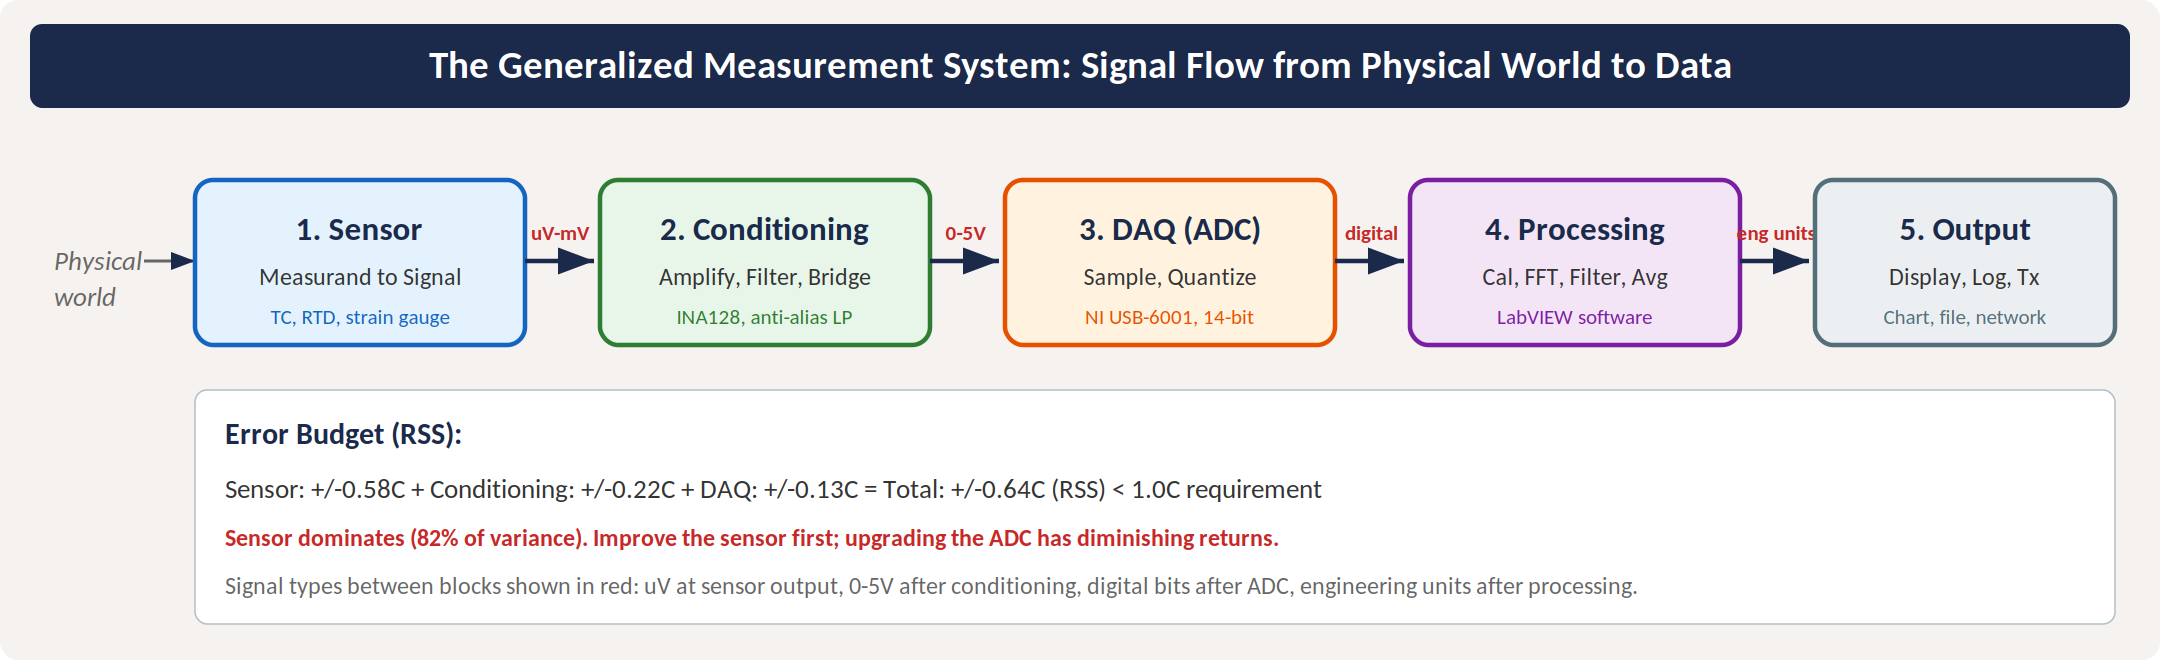
\includegraphics[width=\textwidth]{fig_measurement_system.png}
\caption{The five-block generalized measurement system. Every instrumentation chain follows this architecture.}
\label{fig:meas_system}
\end{figure}

\begin{keyconceptbox}[Requirements Mapping: Measurement System to Shall-Statements]
Each block in the measurement chain generates testable requirements:
\begin{itemize}[nosep,leftmargin=1.5em]
\item ``Measure temperature to $\pm$0.5\,\degC{}'' $\to$ SENS-REQ: Sensor accuracy $\leq \pm$0.3\,\degC{}; COND-REQ: Signal conditioning error $\leq \pm$0.1\,\degC{}; DAQ-REQ: ADC resolution contributes $\leq \pm$0.1\,\degC{}.
\item Error budgets must be allocated across the chain so that the RSS (root-sum-square) total meets the system requirement.
\end{itemize}
\end{keyconceptbox}

\begin{figure}[htbp]
\centering
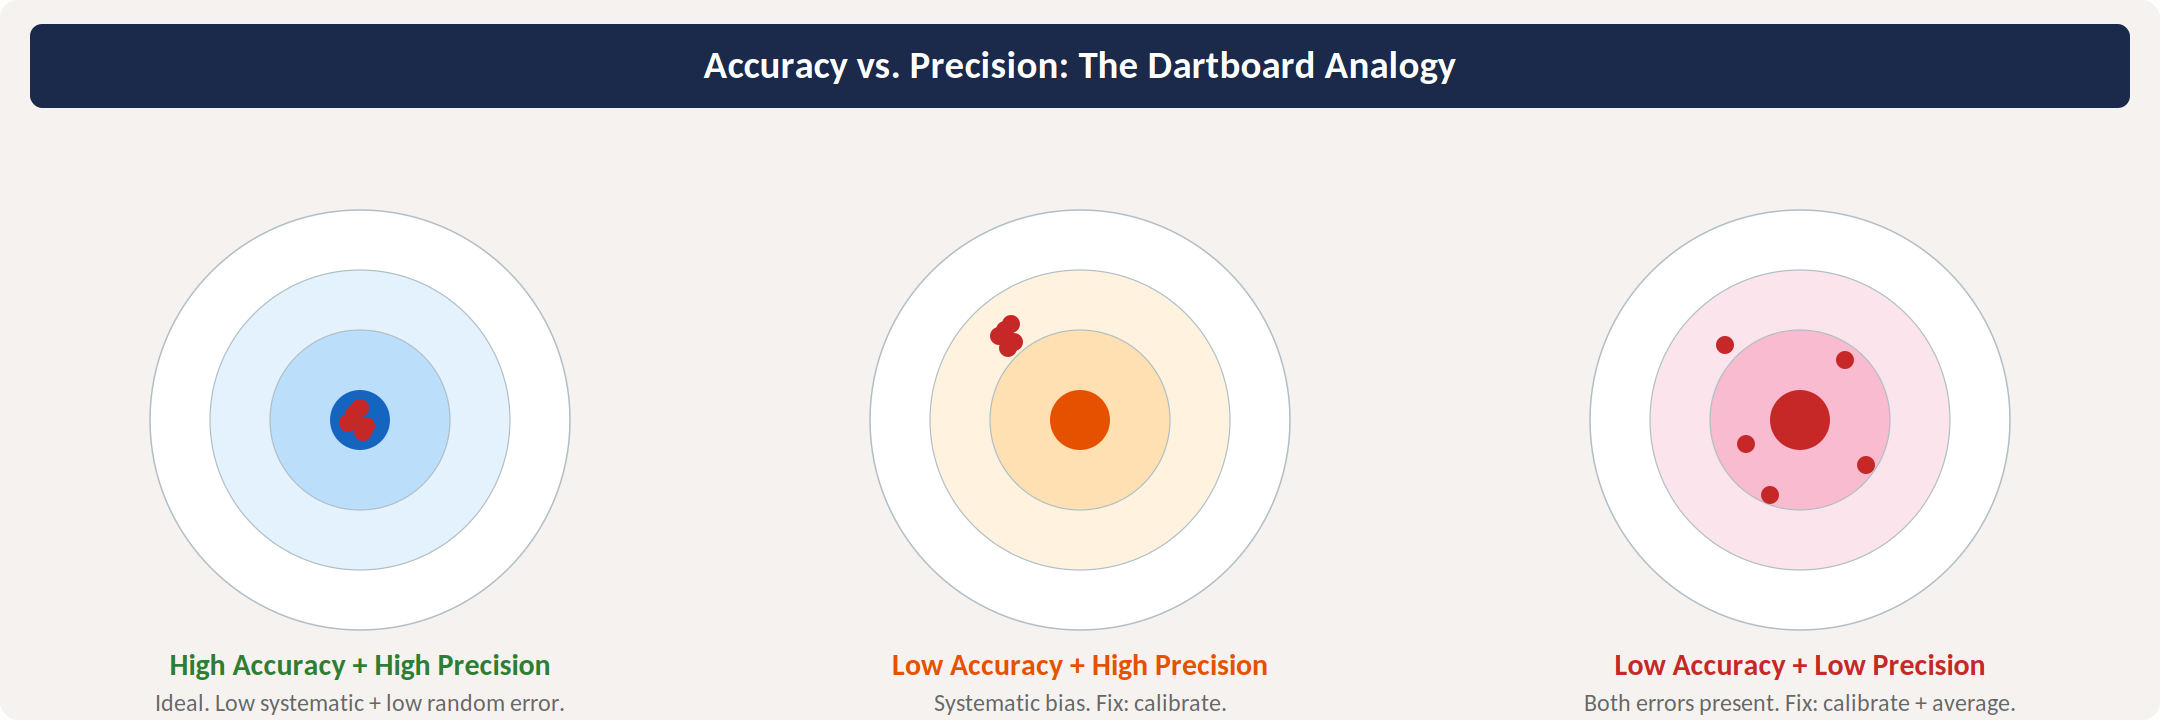
\includegraphics[width=\textwidth]{fig_accuracy_precision.png}
\caption{Accuracy vs.\ precision: the dartboard analogy. High precision with low accuracy (center) indicates systematic bias correctable by calibration. Low precision (right) requires averaging.}
\label{fig:accuracy_precision}
\end{figure}

\section{Sensor Classification}

\subsection{By Energy Source}
\textbf{Active sensors} (self-generating) produce an electrical output from the measurand's energy without external excitation. Examples: thermocouples (Seebeck effect), piezoelectric sensors (mechanical stress $\to$ charge), photovoltaic cells.

\textbf{Passive sensors} require external excitation (voltage or current) and change an electrical property (resistance, capacitance, inductance) in response to the measurand. Examples: RTDs, strain gauges, thermistors, capacitive pressure sensors.

\subsection{By Output Signal}
\textbf{Analog}: output is a continuous voltage or current proportional to the measurand. Requires ADC for digital processing.

\textbf{Digital}: output is a discrete digital word (e.g., I2C, SPI, frequency output). Eliminates the ADC step but shifts the conversion inside the sensor.

\subsection{By Measurand Type}
Temperature (thermocouples, RTDs, thermistors, IR), pressure (diaphragm, piezoelectric, capacitive), force/torque (strain gauge, load cell), displacement (LVDT, potentiometer, encoder, laser), flow (turbine, orifice, ultrasonic, Coriolis), acceleration (MEMS, piezoelectric).

\section{Sensor Terminology}
\begin{table}[htbp]\centering\small
\begin{tabularx}{\textwidth}{l X}
\toprule
\textbf{Term} & \textbf{Definition} \\
\midrule
Range & Span of measurand values the sensor can measure (e.g., 0--100\,\degC{}) \\
Span & Algebraic difference between upper and lower range limits \\
Sensitivity & Output change per unit input change ($S = \Delta y / \Delta x$); slope of the calibration curve \\
Resolution & Smallest detectable change in the measurand \\
Accuracy & Closeness of measured value to true value (includes systematic + random) \\
Precision & Closeness of repeated measurements to each other (random error only) \\
Linearity & Maximum deviation from a best-fit straight line, expressed as \% of full scale \\
Hysteresis & Difference in output for the same input depending on approach direction \\
Repeatability & Variation among successive measurements under identical conditions \\
Drift & Change in output over time with constant input (zero drift and sensitivity drift) \\
Response time & Time to reach a specified percentage (63.2\% or 95\%) of final value after step input \\
\bottomrule
\end{tabularx}
\caption{Essential sensor terminology.}
\end{table}

\begin{warningbox}[Accuracy vs.\ Precision]
A sensor can be precise but inaccurate (consistent readings that are all wrong by the same amount, i.e., a systematic bias). Calibration corrects accuracy. Averaging improves precision. You need both.
\end{warningbox}


\section{Transducer Operating Principles}
Every sensor exploits a physical phenomenon to convert the measurand into a signal. The most important principles in mechanical engineering instrumentation:

\subsection{Resistive}
A change in the measurand produces a change in electrical resistance. Examples: strain gauges (resistance changes with deformation; gauge factor $GF = (\Delta R/R)/\epsilon \approx 2$ for metal foil), RTDs (resistance increases linearly with temperature; $R(T) = R_0[1 + \alpha(T - T_0)]$ where $\alpha \approx 0.00385$\,\degC{}$^{-1}$ for Pt100), thermistors (resistance changes exponentially with temperature; NTC type: resistance decreases as temperature increases), and potentiometers (resistance proportional to wiper position).

\subsection{Thermoelectric}
A temperature difference between two junctions of dissimilar metals generates a voltage (Seebeck effect). Type~K (chromel-alumel): 41\,$\mu$V/\degC{}, range $-200$ to $+1260$\,\degC{}. Type~T (copper-constantan): 43\,$\mu$V/\degC{}, range $-200$ to $+350$\,\degC{}. Requires a \textbf{reference junction} at a known temperature (ice point or electronic cold-junction compensation).

\subsection{Piezoelectric}
Mechanical stress on certain crystals (quartz, PZT ceramics) generates an electric charge proportional to the applied force. Used in accelerometers, pressure sensors, and force sensors. The charge decays over time, so piezoelectric sensors cannot measure static quantities; they are inherently AC-coupled (dynamic measurements only).

\subsection{Capacitive}
A change in plate spacing, overlap area, or dielectric constant changes the capacitance: $C = \epsilon A / d$. Used in MEMS pressure sensors (diaphragm deflection changes $d$), proximity sensors, humidity sensors (dielectric changes with moisture), and MEMS accelerometers.

\subsection{Inductive and Electromagnetic}
LVDTs (Linear Variable Differential Transformers) measure displacement by changing the coupling between a primary and two secondary coils. Excellent linearity, infinite resolution (analog output), and robust construction. Tachometers generate a voltage proportional to rotational speed via electromagnetic induction.

\section{Loading Effects}
Connecting a sensor to a circuit can change the quantity being measured. The sensor draws energy from the measurand, potentially altering it.

\textbf{Electrical loading}: a voltmeter with input impedance $Z_m$ measuring a source with output impedance $Z_s$ reads:
\begin{equation}
V_{\text{measured}} = V_{\text{true}} \times \frac{Z_m}{Z_m + Z_s}
\end{equation}
To keep the loading error below 1\%, require $Z_m > 100 \times Z_s$. This is why buffer amplifiers (Chapter~12) are essential for high-impedance sensors.

\textbf{Thermal loading}: inserting a temperature probe into a small fluid volume changes the fluid temperature. The probe absorbs or releases heat until it equilibrates. In small samples, this thermal mass effect can be significant.

\begin{tipbox}[The 100:1 Impedance Rule]
For voltage measurements, the measuring instrument's input impedance should be at least 100 times the source impedance. For current measurements, the instrument's impedance should be less than 1/100 of the circuit impedance. Violating this rule introduces loading errors that corrupt your data.
\end{tipbox}


\section{Sensor Selection Methodology}
Choosing the right sensor is the single most consequential decision in instrumentation system design. A poor choice propagates through the entire signal chain and cannot be corrected downstream. The selection process follows a systematic hierarchy of constraints.

\subsection{Step 1: Define the Measurand and Environment}
Before evaluating any sensor, define exactly what physical quantity you need to measure and the conditions under which the measurement will occur. Key questions include: what is the expected range of the measurand (minimum to maximum value with margin)? What is the required measurement bandwidth (how fast does the quantity change)? What is the operating environment (temperature extremes, humidity, vibration, chemical exposure, electromagnetic interference)? What mounting constraints exist (size, weight, access)?

\subsection{Step 2: Accuracy and Resolution Requirements}
The system-level accuracy requirement (e.g., ``measure temperature to $\pm$1.0\,\degC{}'') must be decomposed into an error budget allocated across the measurement chain. The sensor typically receives the largest allocation (50--70\% of the total variance budget) because it is the first element and its errors are amplified by subsequent stages. Resolution must be at least 5--10$\times$ finer than the required accuracy to avoid quantization-dominated measurements.

\subsection{Step 3: Dynamic Response Requirements}
If the measurand changes rapidly, the sensor's bandwidth must exceed the signal bandwidth. For first-order sensors, the $-3$\,dB frequency must be at least 5$\times$ the highest signal frequency to keep amplitude error below 1\%. For second-order sensors (accelerometers, pressure transducers), the flat response band extends to approximately $0.2 \times \omega_n$ for a damping ratio of $\zeta = 0.65$. Beyond this frequency, the sensor's output amplitude becomes unreliable.

\subsection{Step 4: Interface Compatibility}
The sensor's output must be compatible with the signal conditioning and DAQ hardware. Key considerations include output type (voltage, current, resistance, frequency, digital bus), output level (millivolts for thermocouples vs.\ volts for integrated sensors), output impedance (high impedance sources require buffer amplifiers), power supply requirements (excitation voltage and current), and wiring configuration (2-wire, 3-wire, or 4-wire for resistance sensors).

\subsection{Step 5: Cost, Availability, and Reliability}
In production systems, sensor cost, lead time, second-source availability, and mean time between failures (MTBF) are critical. In MEGN~300 projects, cost and availability from common distributors (Digi-Key, Mouser, SparkFun, Adafruit) dominate. Always verify that the sensor has a clear, complete datasheet before committing to a design.

\begin{examplebox}[ThermoRig: Sensor Selection Rationale]
For the ThermoRig temperature measurement system, we select a Type~K thermocouple based on the following analysis: the temperature range (ambient to 200\,\degC{}) falls within Type~K's range ($-200$ to $+1260$\,\degC{}). The required accuracy ($\pm$2.2\,\degC{} or $\pm$0.75\%, whichever is greater per ASTM~E230 Standard tolerance) is adequate for our $\pm$1.0\,\degC{} system requirement after calibration reduces the error to $\pm$0.3\,\degC{}. The thermocouple is self-generating (no excitation needed), has a fast response time when using exposed-junction construction ($\tau < 0.5$\,s in moving air), is extremely rugged, and costs less than \$5. The tradeoff: the output is tiny (approximately 41\,$\mu$V/\degC{}), requiring high-gain amplification with excellent common-mode rejection, which we address in Chapter~12.
\end{examplebox}

\section{Measurement System Design Process}
The complete design process for an instrumentation system proceeds through six phases:

\textbf{Phase 1: Requirements Definition.} Write formal ``shall'' statements specifying range, accuracy, resolution, bandwidth, sample rate, output format, environmental limits, and interface requirements. These flow from the system-level measurement objectives.

\textbf{Phase 2: Sensor Selection and Error Budgeting.} Select the sensor technology, allocate the accuracy budget across chain elements, and verify by RSS analysis that the total system uncertainty meets the requirement.

\textbf{Phase 3: Signal Conditioning Design.} Design the amplification, filtering, bridge excitation, and any linearization required to present the sensor signal in the DAQ's input range (typically 0--5\,V or $\pm$10\,V). Choose component values to minimize noise while maintaining the required bandwidth.

\textbf{Phase 4: DAQ Configuration.} Select the sampling rate (at least $10\times$ the signal bandwidth), bit resolution (sufficient that quantization noise is below the sensor noise floor), input mode (differential for millivolt signals, single-ended for volt-level signals), and input range (smallest range that encompasses the conditioned signal to maximize effective resolution).

\textbf{Phase 5: Software Implementation.} Implement the data acquisition loop, real-time calibration equations, digital filtering, display, logging, and any control algorithms in LabVIEW. Verify timing (loop rate, buffer management) and data integrity.

\textbf{Phase 6: Calibration and Validation.} Calibrate the complete system against known standards. Compare measured values to reference instruments across the full operating range. Calculate the actual measurement uncertainty and verify it meets the requirements.

\begin{tipbox}[The Five Questions Every Engineer Asks]
Before designing any measurement system, answer these five questions: (1)~What am I measuring? (2)~How accurately? (3)~How fast is it changing? (4)~What environment will it operate in? (5)~What do I do with the data? The answers to these five questions determine every subsequent design decision.
\end{tipbox}

\section{Units, Standards, and Traceability}
All measurements must be traceable to national or international standards. In the United States, the National Institute of Standards and Technology (NIST) maintains primary measurement standards. Traceability means an unbroken chain of calibrations connecting your measurement to the national standard, with documented uncertainties at each step.

The International System of Units (SI) defines seven base units: meter (length), kilogram (mass), second (time), ampere (electric current), kelvin (temperature), mole (amount of substance), and candela (luminous intensity). All other units are derived from these seven. In instrumentation, the most commonly encountered derived units include pascal (pressure, Pa = N/m$^2$), hertz (frequency, Hz = 1/s), volt (V = W/A), and ohm ($\Omega$ = V/A).

Calibration certificates from accredited laboratories (ISO/IEC~17025) provide the legal basis for measurement traceability. In industrial metrology, calibration intervals are set based on historical drift data, criticality of the measurement, and regulatory requirements. A common starting interval is 12 months, adjusted based on observed stability.

\begin{warningbox}[Significant Figures and Reporting]
Never report a measurement with more significant figures than the uncertainty justifies. If your system uncertainty is $\pm$0.5\,\degC{}, reporting ``23.472\,\degC{}'' is misleading; correct reporting is ``23.5 $\pm$ 0.5\,\degC{}'' or equivalently ``23.5(5)\,\degC{}.'' The number of decimal places in the reported value should match the number of decimal places in the uncertainty.
\end{warningbox}

\section{Sensor Selection Methodology}
Choosing the right sensor is the most consequential decision in instrumentation design. A poor choice propagates through the entire signal chain. The process follows five steps.

\textbf{Step 1: Define measurand and environment.} What is the expected range (with margin)? What is the measurement bandwidth? What is the operating environment (temperature, vibration, chemical exposure, EMI)? What mounting constraints exist?

\textbf{Step 2: Accuracy and resolution.} The system accuracy requirement must be decomposed into an error budget. The sensor typically receives 50--70\% of the variance budget. Resolution must be 5--10$\times$ finer than accuracy.

\textbf{Step 3: Dynamic response.} Sensor bandwidth must exceed signal bandwidth by $5\times$--$10\times$. For first-order sensors, the $-3$\,dB frequency must be $5\times$ the highest signal frequency for $<$1\% amplitude error.

\textbf{Step 4: Interface compatibility.} Output type (voltage, current, resistance, digital), output level, impedance, power requirements, wiring configuration (2/3/4-wire).

\textbf{Step 5: Cost, availability, reliability.} Verify the sensor has a complete datasheet. Check distributor stock and lead time.

\section{Measurement System Design Process}
The six phases: (1) Requirements definition with formal ``shall'' statements. (2) Sensor selection and error budgeting. (3) Signal conditioning design (amplification, filtering, bridge excitation). (4) DAQ configuration (sample rate, bit resolution, input mode, range). (5) Software implementation (LabVIEW: acquisition loop, calibration, filtering, display). (6) Calibration and validation against known standards.

\begin{tipbox}[Five Questions for Every Measurement System]
Before designing: (1) What am I measuring? (2) How accurately? (3) How fast is it changing? (4) What environment? (5) What do I do with the data? These answers determine every subsequent decision.
\end{tipbox}

\section{Units, Standards, and Traceability}
All measurements must be traceable to national standards (NIST in the US). SI base units: meter, kilogram, second, ampere, kelvin, mole, candela. Common derived: pascal (Pa), hertz (Hz), volt (V), ohm ($\Omega$). Calibration certificates from ISO/IEC 17025 accredited labs provide legal traceability. Common calibration interval: 12 months, adjusted based on observed stability.

\begin{warningbox}[Significant Figures]
Never report more significant figures than the uncertainty justifies. If uncertainty is $\pm$0.5\,\degC{}, report ``23.5 $\pm$ 0.5\,\degC{},'' not ``23.472\,\degC{}.'' Match decimal places in value and uncertainty.
\end{warningbox}
\section{Signal Types and Their Characteristics}
Understanding the nature of the signal produced by a sensor is essential for designing the rest of the measurement chain.

\textbf{DC signals} are constant or very slowly varying (temperature from an RTD, pressure from a strain gauge bridge). They require high-accuracy, low-noise amplification and are susceptible to 1/f noise and drift. Typical signal conditioning: instrumentation amplifier with low offset voltage, followed by a low-pass filter with cutoff at 1--10\,Hz.

\textbf{AC signals} vary periodically or quasi-periodically (vibration, acoustic pressure, alternating current). The frequency content carries the information. Signal conditioning emphasizes bandwidth, phase linearity, and noise rejection in the signal band. AC-coupled amplifiers (with a high-pass input filter) reject DC offset and low-frequency drift.

\textbf{Transient signals} are short-duration events (impact force, shock wave, spark discharge). They contain energy spread across a wide frequency band. The measurement system must have sufficient bandwidth to capture the fastest features and sufficient dynamic range to capture both the peak and the fine structure. Triggering (starting the acquisition at the moment of the event) is critical.

\textbf{Pulse signals} are digital or quasi-digital (encoder outputs, frequency-output sensors, PWM signals). They carry information in timing (period, duty cycle, edge count) rather than amplitude. Signal conditioning focuses on edge detection, debouncing, and accurate timing measurement.

\section{Sensor Specifications: What the Numbers Mean}
Datasheet specifications often confuse students because they use different reference conditions, definitions, and statistical bases. Key clarifications:

\textbf{Full Scale Output (FSO)} is the algebraic difference between the output at maximum and minimum measurand values. Many error specifications are expressed as a percentage of FSO. A sensor with 0.1\% FSO accuracy on a 0--1000\,psi range has $\pm$1\,psi error at every point in the range, whether measuring 10\,psi or 990\,psi. This means the relative error at low readings is very large (10\% at 10\,psi).

\textbf{Best Fit Straight Line (BFSL) linearity} expresses nonlinearity as the maximum deviation from a least-squares line through the calibration data. This is the most common specification and the most optimistic. \textbf{End-point linearity} uses the line connecting the zero and full-scale points, which is more conservative and more representative of actual use.

\textbf{Temperature coefficient} specifies how much a parameter (offset, gain, accuracy) changes per degree of temperature change, typically in ppm/\degC{} or \%/\degC{}. A 50\,ppm/\degC{} gain drift on a 200\,\degC{} temperature excursion produces a $50 \times 200 \times 10^{-6} = 1\%$ gain error. This can dominate the error budget in environments with large temperature swings.

\textbf{Long-term stability (drift)} describes how much the output changes over months or years with constant input. Precision sensors specify drift rates of 0.01--0.1\%/year. For field instruments recalibrated annually, long-term drift contributes to the total uncertainty.

\section{Sensor Failure Modes}
Understanding how sensors fail helps you design robust systems:

\textbf{Open circuit}: the sensor connection breaks (wire fatigue, corrosion, connector failure). The measurement reads full-scale or rail voltage. Detection: check for readings at the ADC limit.

\textbf{Short circuit}: two conductors contact (insulation failure, moisture, conductive contamination). The measurement reads zero or a fixed offset. Detection: check for stuck-at-zero readings.

\textbf{Drift}: gradual change in sensitivity or offset due to aging, contamination, or mechanical creep. The measurement appears valid but is increasingly wrong. Detection: periodic recalibration against a reference standard.

\textbf{Saturation}: the measurand exceeds the sensor's range. The output clips at the maximum value, losing the true peak information. Detection: check for readings at or near the full-scale output.

\textbf{Intermittent}: loose connections or cracked solder joints cause sporadic noise spikes or dropouts. Often vibration-dependent. Detection: monitor for statistical outliers in the data stream.

\begin{tipbox}[Design for Diagnosability]
Include self-diagnostic features in your measurement system: range checking (flag readings at ADC limits), rate-of-change checking (flag physically impossible jumps), and periodic reference checks (measure a known voltage to verify the signal chain is functioning). These cost nothing to implement in software and can save hours of debugging.
\end{tipbox}
\section{Measurement in the Engineering Design Process}
Measurements serve different purposes at different project phases, and understanding this shapes how you design your measurement system:

\textbf{Concept phase}: measurements are exploratory. You need rough data to understand the design space and make go/no-go decisions. Accuracy requirements are loose ($\pm$10\%); speed and convenience matter more. Use handheld instruments, default DAQ settings, and minimal signal conditioning.

\textbf{Detailed design phase}: measurements validate models and characterize components. Accuracy tightens ($\pm$1--5\%). Calibration becomes important. Use dedicated signal conditioning, proper anti-alias filtering, and documented calibration procedures.

\textbf{Verification and validation phase}: measurements prove the system meets its requirements. Accuracy is dictated by the requirement specifications. Full calibration, documented uncertainty analysis, and traceable reference standards are mandatory. The measurement uncertainty must be less than $1/4$ of the specification tolerance (4:1 TAR).

\textbf{Production and field phase}: measurements monitor ongoing performance and detect degradation. Emphasis shifts to reliability, automated data collection, and statistical process control. Measurement systems must be robust to operator variation (Gauge R\&R).

\section{Common Measurement Mistakes in Student Projects}
Based on a decade of MEGN~300 lab experience, the most frequent measurement mistakes are:

(1) \textbf{No anti-alias filter}: aliased noise corrupts the data, producing unexplained frequency components. Fix: always include an analog LP filter before the ADC.

(2) \textbf{Wrong input mode}: using RSE (single-ended) for millivolt signals, allowing ground offsets and 60\,Hz to corrupt the measurement. Fix: use Differential for all signals $< 100$\,mV.

(3) \textbf{Wasting ADC range}: measuring a 0--2\,V signal on a $\pm$10\,V range, losing 3+ bits of effective resolution. Fix: match the signal conditioning gain to use 80--90\% of the ADC range.

(4) \textbf{No calibration}: reporting raw sensor output as the measurement, without calibrating against a reference standard. Fix: always calibrate and apply the calibration equation.

(5) \textbf{No uncertainty analysis}: reporting ``$T = 23.47$\,\degC{}'' without stating the uncertainty. Fix: every measurement must include an uncertainty statement.

(6) \textbf{Ignoring sensor dynamics}: measuring a fast-changing quantity with a slow sensor and reporting the attenuated value as correct. Fix: verify that the sensor bandwidth exceeds the signal bandwidth by $5\times$.
\section{Practice Questions}
\begin{enumerate}[leftmargin=1.5em]
\item Draw the five-block generalized measurement system for measuring the vibration of a rotating shaft. Identify a specific sensor, signal conditioning operation, DAQ device, processing step, and output format for each block.
\item A pressure sensor has a range of 0--500\,psi, an output of 0--5\,V, and a stated accuracy of $\pm$0.25\% FS. What is the sensitivity? What is the maximum error in psi?
\item Explain the difference between accuracy and precision using a dartboard analogy. A sensor has high precision but low accuracy. What type of error dominates, and how do you fix it?
\item A thermocouple (active sensor) and an RTD (passive sensor) both measure temperature. Explain the fundamental difference in how they produce their output signals. Which requires external excitation and why?
\item Your measurement system must measure temperature to $\pm$1.0\,\degC{}. Allocate an error budget across the sensor, signal conditioning, and DAQ stages such that the RSS total meets the requirement.
\end{enumerate}

\subsection{Answers}
\begin{enumerate}[leftmargin=1.5em]
\item Sensor: accelerometer (e.g., ADXL345 MEMS). Signal conditioning: charge amplifier + low-pass filter at 1\,kHz. DAQ: NI~USB-6001 at 10\,kS/s, 14-bit. Processing: FFT to identify dominant vibration frequencies. Output: frequency spectrum plot in LabVIEW with peak frequency and amplitude annotations.
\item Sensitivity $S = 5\,\text{V} / 500\,\text{psi} = 0.01\,\text{V/psi} = 10\,\text{mV/psi}$. Accuracy $= \pm 0.25\% \times 500 = \pm 1.25\,\text{psi}$ (or equivalently $\pm 12.5\,\text{mV}$).
\item Precise but inaccurate = all darts clustered together but off-center. Systematic error dominates. Fix: calibrate against a known standard and apply a correction offset (or curve).
\item A thermocouple generates a voltage from the Seebeck effect at the junction of two dissimilar metals; no external power is needed. An RTD changes resistance with temperature but produces no voltage on its own; it requires an excitation current (typically 1\,mA) passed through the element, and the voltage drop is measured to calculate resistance, then converted to temperature.
\item Example allocation: Sensor: $\pm$0.6\,\degC{}, Signal conditioning: $\pm$0.5\,\degC{}, DAQ (quantization + noise): $\pm$0.5\,\degC{}. RSS $= \sqrt{0.6^2 + 0.5^2 + 0.5^2} = \sqrt{0.86} = 0.93\,\degC{} < 1.0\,\degC{}$. Meets requirement.
\end{enumerate}


% ================================================================
\chapter{Static Measurements}

\section{Static Calibration}
Static calibration determines the relationship between the sensor input (measurand) and output (signal) under steady-state conditions, where the measurand is not changing with time. The calibration process produces a \textbf{calibration curve}: a plot or equation mapping input to output.

\subsection{The Calibration Process}
\begin{enumerate}[leftmargin=1.5em]
\item Apply a series of known, stable input values spanning the sensor's range, using a \textbf{calibration standard} with accuracy $\geq 4\times$ better than the sensor under test (4:1 Test Accuracy Ratio, per ANSI/NCSL Z540.3).
\item Record the sensor output at each input value. Allow sufficient settling time at each point.
\item Apply inputs in both increasing and decreasing order to detect hysteresis.
\item Repeat the entire sequence at least 3 times to assess repeatability.
\item Fit a calibration equation (linear, polynomial, or piecewise) to the data.
\item Calculate residuals (measured $-$ predicted) and report maximum error.
\end{enumerate}

\subsection{Linear Calibration}
Most sensors are designed to be approximately linear over their operating range:
\begin{equation}
y = mx + b
\end{equation}
where $y$ = sensor output, $x$ = measurand, $m$ = sensitivity (slope), and $b$ = zero offset (intercept). The sensitivity $m$ and offset $b$ are determined by least-squares regression on the calibration data.

\subsection{Nonlinear Calibration}
Some sensors are inherently nonlinear (e.g., thermistors: $R = R_0 e^{\beta(1/T - 1/T_0)}$). For these, use a polynomial fit ($y = a_0 + a_1 x + a_2 x^2 + \cdots$) or a lookup table with interpolation. The Steinhart-Hart equation provides a three-coefficient model for thermistors that is accurate to $\pm$0.01\,\degC{} over wide ranges.

\begin{examplebox}[ThermoRig: Static Calibration of a Type K Thermocouple]
Calibration standard: NIST-traceable ice point (0.0\,\degC{}) and boiling point (100.0\,\degC{} at local altitude, corrected for barometric pressure in Golden, CO: $\approx$95.0\,\degC{} at 5,675\,ft elevation). Additional points at 25\,\degC{} and 50\,\degC{} using a calibrated water bath.

Calibration equation (linear fit): $T = 24.98 \times V_{mV} + 0.15$\,\degC{}. Residuals: max $\pm$0.8\,\degC{} over 0--95\,\degC{} range. With a second-order polynomial: max residual drops to $\pm$0.3\,\degC{}.
\end{examplebox}

\section{Static Characteristics}

\subsection{Sensitivity}
Sensitivity $S$ is the slope of the calibration curve:
\begin{equation}
S = \frac{\partial y}{\partial x} \approx \frac{\Delta y}{\Delta x}
\end{equation}
Units: output units per input unit (e.g., mV/\degC{}, $\Omega$/kPa). A higher sensitivity produces a larger output change for a given input change, improving resolution and signal-to-noise ratio. For a linear sensor, sensitivity is constant. For a nonlinear sensor, sensitivity varies with the operating point.

\subsection{Linearity}
Linearity error is the maximum deviation of the calibration curve from a reference straight line, expressed as a percentage of full-scale output (FSO):
\begin{equation}
\text{Linearity} = \frac{\max |y_{\text{actual}} - y_{\text{line}}|}{\text{FSO}} \times 100\%
\end{equation}
Three definitions of the reference line exist: \textbf{end-point} (connects the zero and full-scale points), \textbf{best-fit} (least-squares line through all data), and \textbf{independent} (best-fit line not constrained to pass through zero). The independent best-fit method gives the smallest linearity error and is most common in datasheets.

\subsection{Hysteresis}
Hysteresis is the difference in output between the up-sweep (increasing input) and the down-sweep (decreasing input) at the same input value. Causes include mechanical friction, magnetic remanence, and thermal lag. Expressed as \% FSO:
\begin{equation}
\text{Hysteresis} = \frac{\max |y_{\text{up}} - y_{\text{down}}|}{\text{FSO}} \times 100\%
\end{equation}

\subsection{Resolution and Threshold}
\textbf{Resolution} is the smallest input change that produces a detectable output change. For analog sensors, resolution is limited by noise. For digital sensors, resolution is set by the least significant bit (LSB). \textbf{Threshold} is the minimum input required to produce any output at all (relevant for sensors with a dead zone near zero).

\subsection{Drift}
\textbf{Zero drift} (offset drift) is a change in the output at zero input over time or with temperature changes. \textbf{Sensitivity drift} (span drift) is a change in the slope of the calibration curve. Temperature is the most common cause of both. Drift is specified in units per \degC{} or units per year.

\begin{tipbox}[Recalibrate Regularly]
Drift means your calibration degrades over time. Establish a recalibration interval based on the manufacturer's stability specification and the accuracy requirements of your application. For student lab instruments, recalibrate at the start of each semester. For critical measurements, recalibrate before every test series.
\end{tipbox}


\section{Bridge Circuits}
The Wheatstone bridge is the most important circuit in resistive sensor instrumentation. It converts small resistance changes into measurable voltage changes with excellent sensitivity and inherent temperature compensation.

\subsection{The Wheatstone Bridge}
Four resistors arranged in a diamond pattern with excitation voltage $V_{ex}$ applied across one diagonal and the output voltage $V_o$ measured across the other:
\begin{equation}
V_o = V_{ex} \left(\frac{R_1}{R_1 + R_2} - \frac{R_3}{R_3 + R_4}\right)
\end{equation}
When the bridge is balanced ($R_1/R_2 = R_3/R_4$), $V_o = 0$. A small change $\Delta R$ in one arm produces:
\begin{equation}
\Delta V_o \approx \frac{V_{ex}}{4} \cdot \frac{\Delta R}{R} \quad \text{(quarter-bridge)}
\end{equation}

\subsection{Bridge Configurations}
\textbf{Quarter-bridge}: one active gauge, three fixed resistors. Simplest; output proportional to strain. Sensitive to temperature unless a dummy gauge is used in an adjacent arm.

\textbf{Half-bridge}: two active gauges in adjacent arms. Doubles sensitivity and provides automatic temperature compensation if both gauges experience the same temperature.

\textbf{Full-bridge}: four active gauges. Quadruples sensitivity, provides full temperature compensation, and rejects bending strains (if configured for axial measurement). Used in commercial load cells.

\begin{figure}[htbp]
\centering
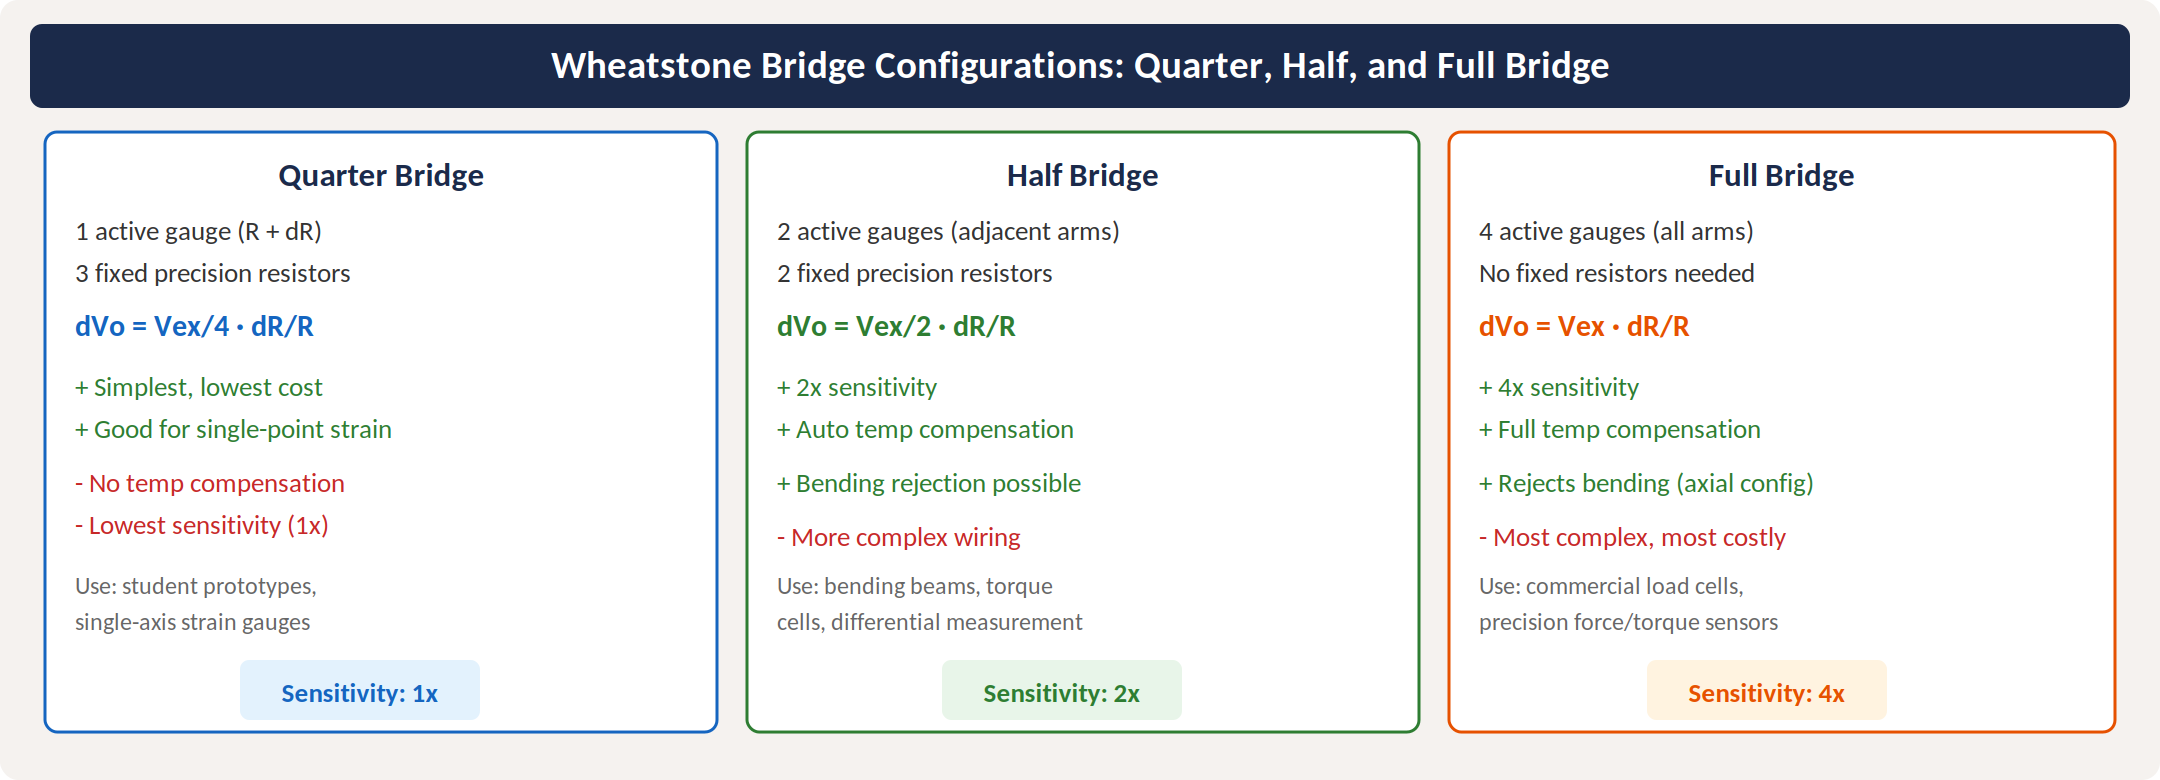
\includegraphics[width=\textwidth]{fig_wheatstone_bridge.png}
\caption{Wheatstone bridge configurations. Sensitivity doubles with each step: quarter-bridge $\Delta V \approx V_{ex}(\Delta R/R)/4$, half-bridge $\Delta V \approx V_{ex}(\Delta R/R)/2$, full-bridge $\Delta V \approx V_{ex}(\Delta R/R)$. Full bridge also provides complete temperature compensation.}
\label{fig:bridge}
\end{figure}

\begin{examplebox}[ThermoRig: RTD in a Wheatstone Bridge]
A Pt100 RTD ($R_0 = 100.0\,\Omega$ at 0\,\degC{}, $\alpha = 0.00385$\,\degC{}$^{-1}$) is placed in a quarter-bridge with $V_{ex} = 5.0$\,V and three 100.0\,$\Omega$ precision resistors. At 25\,\degC{}: $R_{RTD} = 100(1 + 0.00385 \times 25) = 109.6\,\Omega$. Bridge output: $V_o = 5.0 \times (109.6/(109.6+100) - 100/(100+100)) = 5.0 \times (0.5229 - 0.5000) = 114.5$\,mV. Sensitivity: 114.5\,mV / 25\,\degC{} = 4.58\,mV/\degC{}.

Self-heating check: bridge current through RTD $= V_{ex}/(2R) \approx 25$\,mA. Power dissipated in RTD $= I^2 R = 0.025^2 \times 110 = 0.069$\,W. Self-heating coefficient for a Pt100 in still air $\approx$ 0.5\,\degC{}/mW $\to$ self-heating error $= 0.069 \times 0.5 = 0.035$\,\degC{}. Acceptable for $\pm$0.5\,\degC{} accuracy, but reduce $V_{ex}$ to 1\,V for higher precision.
\end{examplebox}

\section{Calibration Standards and Traceability}
A calibration is only as good as the reference standard. \textbf{Traceability} means the calibration chain can be traced back to a national or international standard through an unbroken series of comparisons, each with documented uncertainty.

\begin{itemize}[leftmargin=1.5em]
\item \textbf{Primary standards}: defined by fundamental physics (triple point of water = 273.16\,K exactly; NIST maintains primary standards for all SI units).
\item \textbf{Secondary/transfer standards}: calibrated against primary standards. Used by calibration laboratories.
\item \textbf{Working standards}: calibrated against secondary standards. Used in the lab to calibrate sensors.
\item \textbf{Test Accuracy Ratio (TAR)}: the standard should be $\geq$4$\times$ more accurate than the device under test (4:1 TAR per ANSI/NCSL Z540.3).
\end{itemize}


\section{Fundamentals of Calibration}
Calibration establishes the relationship between sensor output and true measurand value by applying known reference stimuli. Without calibration, a sensor's output is a raw electrical signal with no physical meaning.

\subsection{Calibration Standards and Traceability}
The reference standard must be at least 4$\times$ more accurate than the sensor under calibration (4:1 test accuracy ratio). Common standards: ice-point baths (0.000\,\degC{} $\pm$0.002\,\degC{}), dead-weight testers (pressure), precision decade resistors, certified mass sets. All standards must be traceable to NIST through an unbroken chain of documented calibrations.

\subsection{Static Calibration Procedure}
(1) Thermal equilibrium (15+ minutes after power-on). (2) Apply 5--7 known inputs spanning the full range. (3) Record sensor output at each. (4) Repeat sweep in reverse (detect hysteresis). (5) Repeat 3--5 times (quantify repeatability). (6) Fit calibration curve. (7) Calculate residuals and report uncertainty.

\subsection{Linear vs.\ Polynomial Calibration}
For linear sensors (RTDs, LVDTs): $y = mx + b$ via least-squares regression. Sensitivity $m$ and offset $b$. For nonlinear sensors (thermistors, wide-range thermocouples): polynomial $y = a_0 + a_1 x + a_2 x^2 + \cdots + a_n x^n$ using LabVIEW's General Polynomial Fit VI. Report the goodness-of-fit $R^2$.

\begin{warningbox}[Do Not Extrapolate Beyond Calibration Range]
A calibration curve is valid only within the range of inputs used to generate it. Beyond this range, the sensor may saturate, exhibit unexpected nonlinearity, or produce physically meaningless outputs. Always recalibrate over a wider range if measurements approach the boundaries.
\end{warningbox}

\begin{examplebox}[ThermoRig: Type K Thermocouple Calibration]
Five calibration points: ice bath (0\,\degC{}), room temperature (23\,\degC{} from NIST-traceable reference), warm water at 50\,\degC{}, 75\,\degC{}, and boiling water (100\,\degC{} adjusted for altitude: $T_{bp} = 100 - 0.037(760 - P_{mmHg})$). At each point, 100 samples (10\,s at 10\,S/s), mean computed. Linear fit: $T = 24.12 \times V_{mV} + 0.31$, $R^2 = 0.9998$, max residual 0.28\,\degC{}. Calibration uncertainty: $\pm$0.3\,\degC{} (95\% confidence).
\end{examplebox}

\section{The Wheatstone Bridge in Detail}
\subsection{Bridge Theory}
Four resistors in a diamond, excitation voltage $V_{ex}$ across one diagonal, output $V_o$ across the other. For balanced bridge (all $R$ equal): $V_o = 0$. With one arm changed by $\Delta R$ (quarter bridge):
\begin{equation}
V_o \approx \frac{V_{ex}}{4} \cdot \frac{\Delta R}{R} \quad (\Delta R \ll R)
\end{equation}

\subsection{Bridge Nonlinearity}
The exact output: $V_o = (V_{ex}/4) \cdot (\Delta R/R)/(1 + \Delta R/(2R))$. For $\Delta R/R = 1\%$: 0.5\% nonlinearity. For 10\%: 5\%. Half and full bridges cancel this.

\subsection{Lead Wire Compensation}
Remote sensors add series lead resistance that offsets and desensitizes the bridge. Three-wire connection: adds equal lead resistance to adjacent arm, canceling the effect. Four-wire (Kelvin): eliminates lead resistance entirely using separate current and voltage pairs.

\section{Signal Conditioning for Static Measurements}
\textbf{Amplification}: INA maps bridge output ($\pm$10\,mV typical) to DAQ range. For $\pm$10\,mV to $\pm$5\,V: $G = 500$.

\textbf{Anti-alias filtering}: LP filter at 10--100\,Hz for static measurements removes wideband noise.

\textbf{Excitation regulation}: bridge sensitivity is proportional to $V_{ex}$. Use precision voltage reference (e.g., REF5050 for 5.000\,V $\pm$0.05\%), not a bench supply.

\begin{tipbox}[Self-Heating in Resistance Sensors]
Excitation current through RTDs/thermistors generates Joule heating ($P = I^2 R$) raising sensor temperature above the measurand. For Pt100 at 1\,mA: 0.1--1\,\degC{} self-heating depending on thermal coupling. Use the minimum excitation current that produces a measurable voltage.
\end{tipbox}

\section{Traceability and Measurement Audit Trail}
Every calibration must be documented: date/time, reference standard (certificate number, expiration), environmental conditions (ambient T, humidity), raw data, calibration equation with coefficients, residuals and uncertainty, operator name. Include calibration records in your engineering logbook and reference them in reports.


\section{Advanced Calibration Techniques}
\subsection{Multi-Point Calibration with Uncertainty Bands}
For high-accuracy applications, calibrate at 10--20 points across the range. At each point, acquire enough samples ($N \geq 30$) to compute the mean and standard deviation. Plot the calibration curve with $\pm 2\sigma$ uncertainty bands. Any point where the measurement falls outside the band indicates a problem (sensor nonlinearity, environmental interference, or reference standard error).

\subsection{In-Situ Calibration}
When possible, calibrate the sensor in its actual operating environment (mounted in the test fixture, wired to the DAQ, with the same cable lengths and routing). This captures installation effects (strain from mounting, thermal coupling, EMI environment) that a bench calibration misses. For the ThermoRig, this means calibrating the thermocouple while it is installed in the thermal specimen holder, not on the bench.

\subsection{Two-Point vs.\ Multi-Point Calibration}
A two-point calibration (zero and span) assumes the sensor is linear and only corrects for offset and gain errors. This is adequate for sensors with specified linearity better than the required accuracy. For sensors with significant nonlinearity (thermistors, some pressure sensors), multi-point calibration with polynomial fitting is necessary. The polynomial order should be the minimum that reduces residuals below the target accuracy; overfitting (too high an order) creates oscillations between calibration points.

\section{Resistance Measurement Techniques}
Many sensors are resistive (strain gauges, RTDs, thermistors, potentiometers). Measuring resistance accurately requires careful technique.

\subsection{Two-Wire Measurement}
The simplest method: pass a known current through the sensor and measure the voltage across it. Problem: the voltage includes the drop across the lead wires ($V = I(R_{\text{sensor}} + 2R_{\text{lead}})$). For a Pt100 RTD ($R = 100\,\Omega$) with 10\,m of 24\,AWG copper wire ($R_{\text{lead}} = 0.85\,\Omega$ per wire), the lead resistance is $1.7\,\Omega$, a 1.7\% error that changes with temperature (copper has $\alpha = 0.00393$/\degC{}).

\subsection{Three-Wire Measurement}
Adds a third wire to sense the voltage at the far end of one lead. The bridge circuit uses the third wire to compensate for lead resistance in one arm. This cancels the lead resistance to first order (assumes both leads have equal resistance). Accuracy improves from 1.7\% to approximately 0.05\% (limited by lead resistance mismatch).

\subsection{Four-Wire (Kelvin) Measurement}
The gold standard: separate pairs of wires carry the excitation current and sense the voltage. The voltage sense wires carry negligible current, so their resistance does not affect the measurement. The measured voltage is exactly $V = I \times R_{\text{sensor}}$, independent of lead resistance. Required for precision RTD measurements ($<$0.01\% accuracy) and any sensor more than a few meters from the DAQ.

\section{Signal Conditioning Chain Design}
The complete signal conditioning chain from sensor to ADC must be designed as an integrated system. Key design decisions and their interactions:

\textbf{Gain allocation}: if total gain of 1000 is needed, splitting it as $100 \times 10$ (first stage $\times$ second stage) is better than $1000 \times 1$ because: (1) the first stage amplifies the signal above the noise floor of the second stage, (2) each stage operates at lower gain, reducing the impact of gain error and bandwidth limitations, and (3) the anti-alias filter can be placed between stages at an intermediate voltage level.

\textbf{Filter placement}: the anti-alias filter should be placed after the last amplification stage and immediately before the ADC. This ensures the filter operates on a signal with good SNR (already amplified) and that no noise is added after filtering.

\textbf{Power supply sequencing}: if the signal conditioning circuit is powered from the same supply as the actuators (heaters, motors), power supply transients from actuator switching can inject noise into the signal chain. Use separate, filtered power supplies for analog and digital/power circuits.

\begin{examplebox}[ThermoRig: Complete Measurement Uncertainty Budget]
The final ThermoRig measurement system, after calibration, has the following uncertainty contributors at the 80\,\degC{} operating point:

Thermocouple calibration residual: $\pm$0.28\,\degC{} (from 5-point linear fit).

Cold junction compensation: $\pm$0.10\,\degC{} (from the AD595 CJC IC accuracy).

INA128 gain error: $\pm$0.05\% $\times$ 80\,\degC{} $= \pm$0.04\,\degC{}.

INA128 offset: 50\,$\mu$V $\times$ 611 gain $= 30.5$\,mV, equivalent to $\pm$0.01\,\degC{} after calibration.

ADC quantization: $\pm$0.5 LSB $= \pm$0.15\,mV $\to \pm$0.004\,\degC{} (negligible).

Total (RSS): $\sqrt{0.28^2 + 0.10^2 + 0.04^2 + 0.01^2 + 0.004^2} = 0.30$\,\degC{}.

This meets the $\pm$0.5\,\degC{} system requirement with 40\% margin. The thermocouple calibration dominates the budget; improving the ADC would have no measurable effect.
\end{examplebox}

\section{Strain Measurement in Detail}
Strain gauges are the most common resistive sensor in mechanical engineering. A metal foil gauge bonded to a structure changes resistance proportionally to strain:
\begin{equation}
\frac{\Delta R}{R} = GF \times \epsilon
\end{equation}
where $GF$ (gauge factor) is approximately 2.0 for metal foil gauges and $\epsilon$ is the mechanical strain (dimensionless, typically expressed in microstrain, $\mu\epsilon = 10^{-6}$).

For a typical strain of 1000\,$\mu\epsilon$ ($= 0.1\%$): $\Delta R/R = 2.0 \times 0.001 = 0.2\%$. For a 120\,$\Omega$ gauge: $\Delta R = 0.24\,\Omega$. In a quarter-bridge with 10\,V excitation: $\Delta V = 10 \times 0.002/4 = 5$\,mV. This tiny signal requires careful amplification and noise rejection.

\subsection{Gauge Installation}
The quality of the gauge bond determines measurement accuracy. Clean the surface with solvent (acetone, then isopropanol). Abrade lightly with 320-grit sandpaper. Apply a thin, uniform layer of cyanoacrylate (strain gauge cement). Position the gauge and clamp for 60 seconds. Verify electrical continuity ($R = 120 \pm 0.5\,\Omega$ for a 120\,$\Omega$ gauge). Any air bubble, misalignment, or excess adhesive degrades the measurement.

\subsection{Temperature Compensation}
Thermal expansion of the structure and the gauge causes apparent strain that is not due to mechanical loading. A quarter-bridge on a steel beam sees approximately $23\,\mu\epsilon$/\degC{} from thermal effects alone. The half-bridge compensates: mount two gauges on the same material; one active (in the strain field), one passive (nearby but unstrained). Temperature affects both equally, canceling in the bridge output.
\section{Sensor Fusion and Redundancy}
When a single sensor cannot meet the accuracy or reliability requirement, combining multiple sensors improves performance. \textbf{Homogeneous redundancy}: multiple identical sensors measuring the same quantity, with outputs averaged to reduce random noise by $\sqrt{N}$. Also provides fault detection: if one sensor deviates significantly from the others, it is likely faulty. \textbf{Heterogeneous fusion}: combining different sensor types (e.g., thermocouple for fast response + RTD for accuracy). A Kalman filter or complementary filter can combine them optimally, using each sensor's strengths.

In MEGN~300 projects, the simplest form of sensor fusion is comparing your primary measurement to an independent check instrument (reference thermometer, multimeter, calibrated pressure gauge). This does not improve your primary measurement but validates it.

\section{Environmental Effects on Static Measurements}
Temperature affects virtually every component in the measurement chain. Strain gauge resistance changes with temperature (apparent thermal strain). Op-amp offset voltage drifts (typically 1--10\,$\mu$V/\degC{}). Resistor values drift (25--100\,ppm/\degC{} for metal film). ADC reference voltage drifts (1--50\,ppm/\degC{}).

For outdoor or industrial measurements, design for the full expected temperature range. Compute the worst-case drift for each component and include it in the error budget. For laboratory measurements, controlling the ambient temperature to $\pm$2\,\degC{} (typical HVAC) usually keeps thermal effects negligible.

Humidity affects: capacitive sensors directly; high-impedance circuits (leakage currents across PCB surfaces); and hygroscopic materials (some strain gauge adhesives absorb moisture, causing drift). Conformal coating protects PCBs in humid environments.

\section{Data Logging Best Practices}
Static measurements often run for hours, days, or weeks. Data integrity requires: (1)~timestamp every sample with a real-time clock (not just sample count), (2)~log raw data (before calibration equations) so you can recalibrate offline, (3)~flush data to disk periodically (every 1--10\,s) to prevent data loss on power failure, (4)~include metadata in the file header (sensor type, calibration date, DAQ settings, operator name), (5)~use binary file formats (TDMS, HDF5) for large datasets rather than CSV (which is 3--10$\times$ larger).
\section{Advanced Bridge Techniques}
\subsection{AC Bridge Excitation}
For high-impedance sensors (semiconductor strain gauges, capacitive sensors), AC excitation offers advantages over DC: (1) eliminates thermoelectric offset voltages (thermocouples at connections produce DC errors that are rejected by AC demodulation), (2) enables capacitive and inductive measurements (which require AC), and (3) allows the use of transformer coupling for galvanic isolation.

The bridge is excited with a sine wave (typically 1--10\,kHz), and the output is demodulated (multiplied by the excitation waveform and low-pass filtered) to extract the DC component proportional to the measurand. This is essentially lock-in detection applied to the bridge, providing excellent noise rejection.

\subsection{Auto-Balancing Bridge}
In a conventional bridge, the output voltage is proportional to $\Delta R/R$, but also depends on the excitation voltage $V_{ex}$. An \textbf{auto-balancing} (or servo-balanced) bridge uses a feedback loop to drive the bridge output to zero by adjusting a reference element. The value of the reference element at balance equals the unknown sensor resistance. This technique eliminates the nonlinearity of the unbalanced bridge and removes sensitivity to excitation voltage variations. Commercial LCR meters and precision resistance bridges use this technique.

\section{Sensor Selection: Decision Matrix}
For temperature measurement, the choice among thermocouple, RTD, thermistor, and IC sensor involves multiple tradeoffs:

\begin{table}[htbp]\centering\small
\begin{tabularx}{\textwidth}{l c c c c}
\toprule
\textbf{Property} & \textbf{Thermocouple} & \textbf{RTD (Pt100)} & \textbf{Thermistor} & \textbf{IC (LM35)} \\
\midrule
Range & $-200$ to $+1260$\,\degC{} & $-200$ to $+850$ & $-40$ to $+300$ & $-55$ to $+150$ \\
Accuracy (uncal.) & $\pm$2.2\,\degC{} & $\pm$0.3\,\degC{} & $\pm$0.2\,\degC{} & $\pm$0.5\,\degC{} \\
Sensitivity & 41\,$\mu$V/\degC{} & 0.385\,$\Omega$/\degC{} & $-$4\%/\degC{} & 10\,mV/\degC{} \\
Linearity & Fair & Excellent & Poor & Excellent \\
Response time & 0.1--10\,s & 1--50\,s & 0.1--10\,s & 1--5\,s \\
Self-heating & None & Yes (excitation) & Yes (excitation) & Yes (bias current) \\
Cost & \$1--\$10 & \$10--\$50 & \$1--\$5 & \$1--\$3 \\
\bottomrule
\end{tabularx}
\caption{Temperature sensor comparison. Thermocouples excel in range and speed; RTDs in accuracy; thermistors in sensitivity; IC sensors in ease of use.}
\end{table}

The selection depends on the application priority: if you need to measure above 300\,\degC{}, only thermocouples and RTDs are options. If you need 0.01\,\degC{} resolution, the thermistor's 4\%/\degC{} sensitivity is best. If you need simple, no-conditioning interface: the IC sensor outputs mV directly, readable by any ADC.

\section{Calibration Transfer Standards}
When your reference standard cannot be brought to the measurement location (e.g., an ice-point bath cannot be used in a vibration test cell), a \textbf{transfer standard} bridges the gap. The transfer standard is calibrated against the primary reference in the lab, then transported to the field and used to calibrate the working sensor.

The transfer standard must be more stable than accurate: it does not need to hold an exact value, but the value must not change between calibration and use. For temperature: a precision platinum RTD in a protective housing, calibrated to $\pm$0.05\,\degC{}, stable to $\pm$0.01\,\degC{}/year. For voltage: a precision voltage reference (Fluke 732A), stable to $\pm$1\,ppm/year.
\section{Practice Questions}
\begin{enumerate}[leftmargin=1.5em]
\item A pressure sensor is calibrated with the following data: (0\,psi, 0.02\,V), (100\,psi, 1.01\,V), (200\,psi, 2.03\,V), (300\,psi, 2.98\,V), (400\,psi, 4.02\,V), (500\,psi, 4.99\,V). Calculate the sensitivity and linearity error (\% FSO) using the end-point line.
\item A thermistor has the Steinhart-Hart coefficients $A = 1.125 \times 10^{-3}$, $B = 2.347 \times 10^{-4}$, $C = 0.856 \times 10^{-7}$ (all in $\text{K}^{-1}$). The measured resistance is 10.0\,k$\Omega$. Calculate the temperature in \degC{}.
\item During calibration of a load cell, the readings during the up-sweep and down-sweep at 250\,N are 2.48\,mV/V and 2.53\,mV/V respectively. Full-scale output is 3.00\,mV/V. Calculate the hysteresis as \% FSO.
\item Your measurement system has a 12-bit ADC with a $\pm$5\,V input range. What is the voltage resolution (LSB)? If the sensor sensitivity is 10\,mV/\degC{}, what is the temperature resolution?
\end{enumerate}

\subsection{Answers}
\begin{enumerate}[leftmargin=1.5em]
\item End-point line: slope $= (4.99 - 0.02)/(500 - 0) = 9.94\,\text{mV/psi}$, intercept $= 0.02\,\text{V}$. Predicted at each point: 0.02, 1.014, 2.008, 3.002, 3.996, 4.99. Residuals: 0, $-$0.004, 0.022, $-$0.022, 0.024, 0. Max $|$residual$|$ = 0.024\,V. FSO = 4.97\,V. Linearity = $0.024/4.97 \times 100 = 0.48\%$ FSO. Sensitivity = 9.94\,mV/psi.
\item $1/T = A + B \ln R + C (\ln R)^3 = 1.125 \times 10^{-3} + 2.347 \times 10^{-4} \times \ln(10000) + 0.856 \times 10^{-7} \times (\ln 10000)^3$. $\ln(10000) = 9.2103$. $1/T = 1.125 \times 10^{-3} + 2.161 \times 10^{-3} + 6.69 \times 10^{-5} = 3.353 \times 10^{-3}$. $T = 298.2\,\text{K} = 25.1$\,\degC{}.
\item Hysteresis $= |2.53 - 2.48| / 3.00 \times 100 = 1.67\%$ FSO.
\item LSB $= 10\,\text{V} / 2^{12} = 10/4096 = 2.44\,\text{mV}$. Temperature resolution $= 2.44\,\text{mV} / 10\,\text{mV/\degC{}} = 0.244\,$\degC{}.
\end{enumerate}


% ================================================================
\chapter{Dynamic Measurements}

\section{Why Dynamic Response Matters}
Static calibration tells you the sensor's input-output relationship when the measurand is constant. But in real systems, measurands change with time: a pressure pulse, a temperature transient, a vibrating structure. A sensor's \textbf{dynamic response} determines how faithfully it tracks a time-varying input. A sensor that responds too slowly will attenuate rapid changes and introduce phase delay.

\section{System Order and Models}

\subsection{Zero-Order Systems}
Output is directly proportional to input at all times: $y(t) = K \cdot x(t)$. The output tracks the input instantaneously with no delay or distortion. Pure zero-order sensors are idealizations, but a wire-wound potentiometer measuring slow displacement is approximately zero-order.

\subsection{First-Order Systems}
Described by:
\begin{equation}
\tau \frac{dy}{dt} + y = K \cdot x(t)
\end{equation}
where $\tau$ is the \textbf{time constant} and $K$ is the static sensitivity. First-order systems are characterized by a single energy storage element (e.g., thermal mass of a temperature probe).

\textbf{Step response}: $y(t) = K \cdot x_0 (1 - e^{-t/\tau})$. After one time constant ($t = \tau$), the output reaches 63.2\% of its final value. After $5\tau$, the output is within 0.7\% of final (effectively settled).

\textbf{Frequency response}: the magnitude ratio and phase are:
\begin{align}
M(\omega) &= \frac{K}{\sqrt{1 + (\omega\tau)^2}} \\
\phi(\omega) &= -\arctan(\omega\tau)
\end{align}
The $-3$\,dB bandwidth (where $M$ drops to $K/\sqrt{2}$) occurs at $\omega = 1/\tau$, or $f_{-3\text{dB}} = 1/(2\pi\tau)$.

\begin{figure}[htbp]
\centering
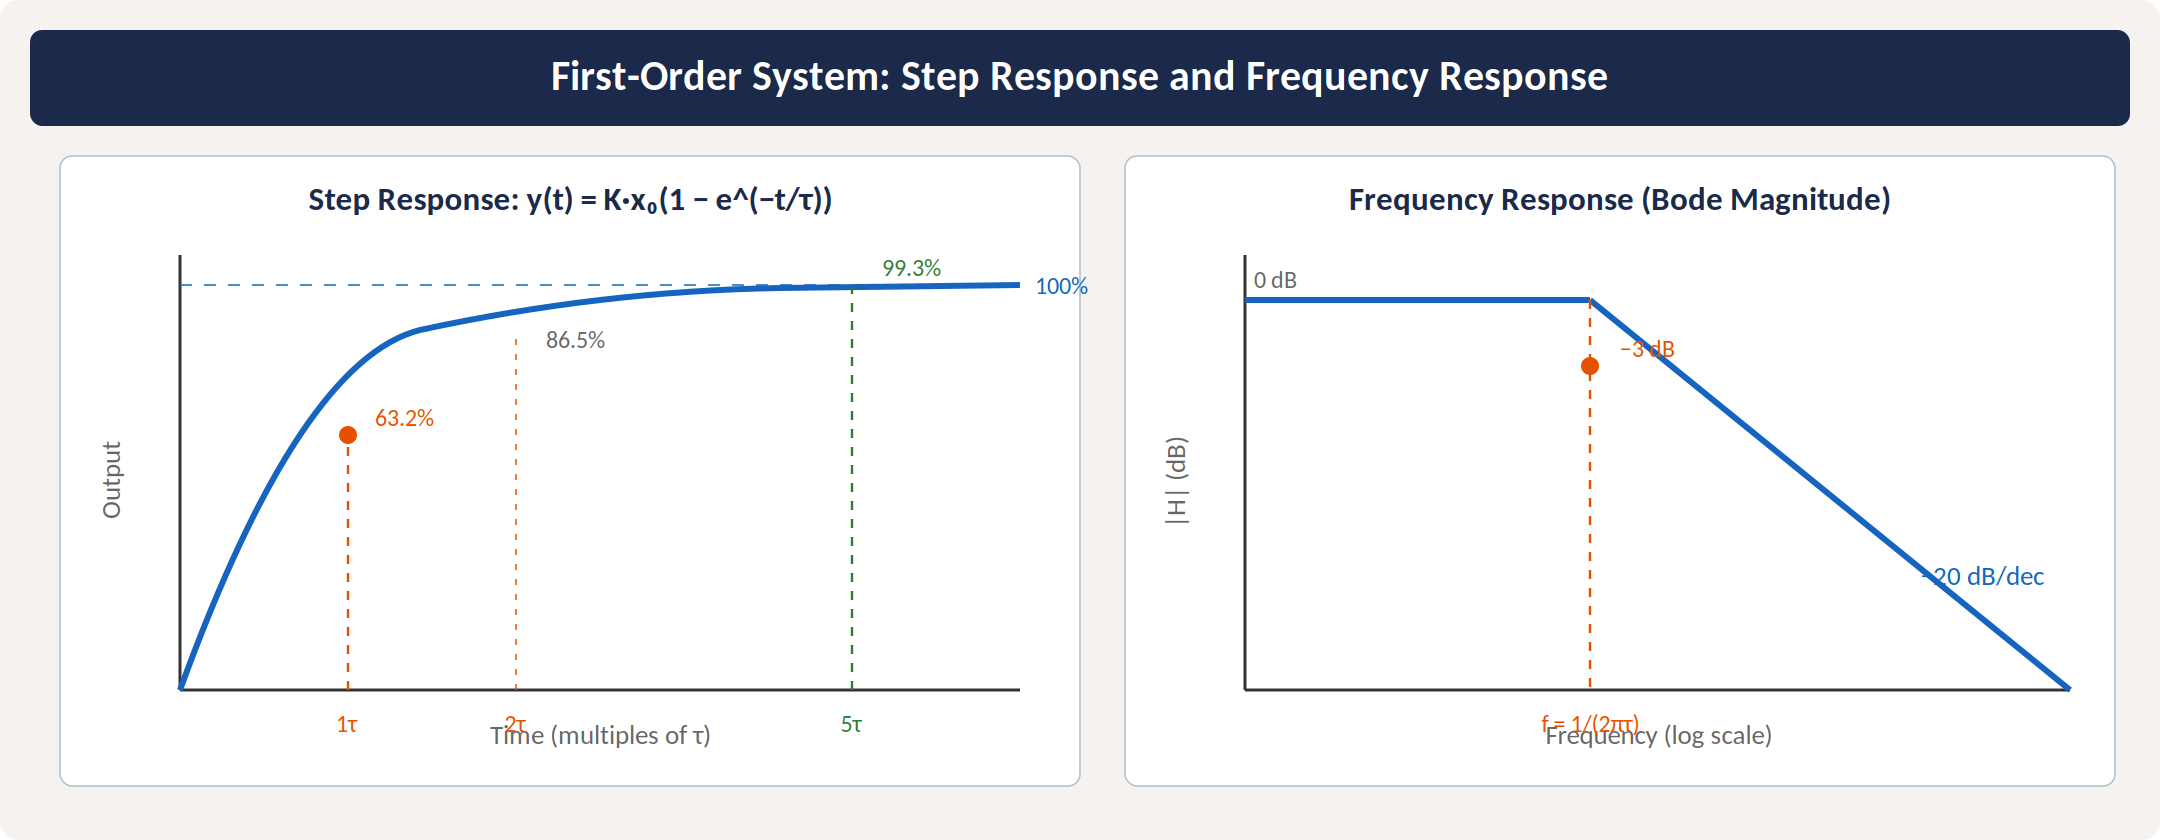
\includegraphics[width=\textwidth]{fig_first_order_response.png}
\caption{First-order system step response (left) and Bode magnitude plot (right). The time constant $\tau$ determines both the settling time ($5\tau$ to 99\%) and the bandwidth ($f_{-3\text{dB}} = 1/2\pi\tau$).}
\label{fig:first_order}
\end{figure}

\begin{examplebox}[ThermoRig: Time Constant of a Thermocouple]
A Type K thermocouple (0.5\,mm bead) plunged into boiling water responds with $\tau \approx 0.2$\,s. This means it reaches 63.2\% of the temperature change in 0.2\,s and settles to within 1\% in $5\tau = 1.0$\,s.

For measuring a temperature that oscillates at 1\,Hz: $\omega = 2\pi$, $\omega\tau = 1.26$, $M = K/\sqrt{1 + 1.59} = 0.62K$. The sensor attenuates the oscillation to 62\% of its true amplitude and introduces a $-51.6$\ang{} phase lag. The measurement significantly underreports the true oscillation.

\textbf{Lesson}: to faithfully measure a 1\,Hz temperature oscillation, you need $\tau \ll 1/(2\pi \times 1) = 0.16$\,s. A finer thermocouple (0.1\,mm bead, $\tau \approx 0.01$\,s) would be adequate.
\end{examplebox}

\subsection{Second-Order Systems}
Described by:
\begin{equation}
\frac{1}{\omega_n^2}\frac{d^2 y}{dt^2} + \frac{2\zeta}{\omega_n}\frac{dy}{dt} + y = K \cdot x(t)
\end{equation}
where $\omega_n$ is the \textbf{undamped natural frequency} and $\zeta$ is the \textbf{damping ratio}. Typical second-order sensors: accelerometers, pressure transducers with diaphragms, and force sensors with spring elements.

Three damping regimes: \textbf{underdamped} ($\zeta < 1$): oscillatory response with overshoot; \textbf{critically damped} ($\zeta = 1$): fastest non-oscillatory response; \textbf{overdamped} ($\zeta > 1$): slow, no oscillation. Most practical sensors target $\zeta \approx 0.6$--$0.7$ for fast response with minimal overshoot ($<$5\%).

\textbf{Frequency response} magnitude:
\begin{equation}
M(\omega) = \frac{K}{\sqrt{[1 - (\omega/\omega_n)^2]^2 + [2\zeta\omega/\omega_n]^2}}
\end{equation}
\begin{figure}[htbp]
\centering
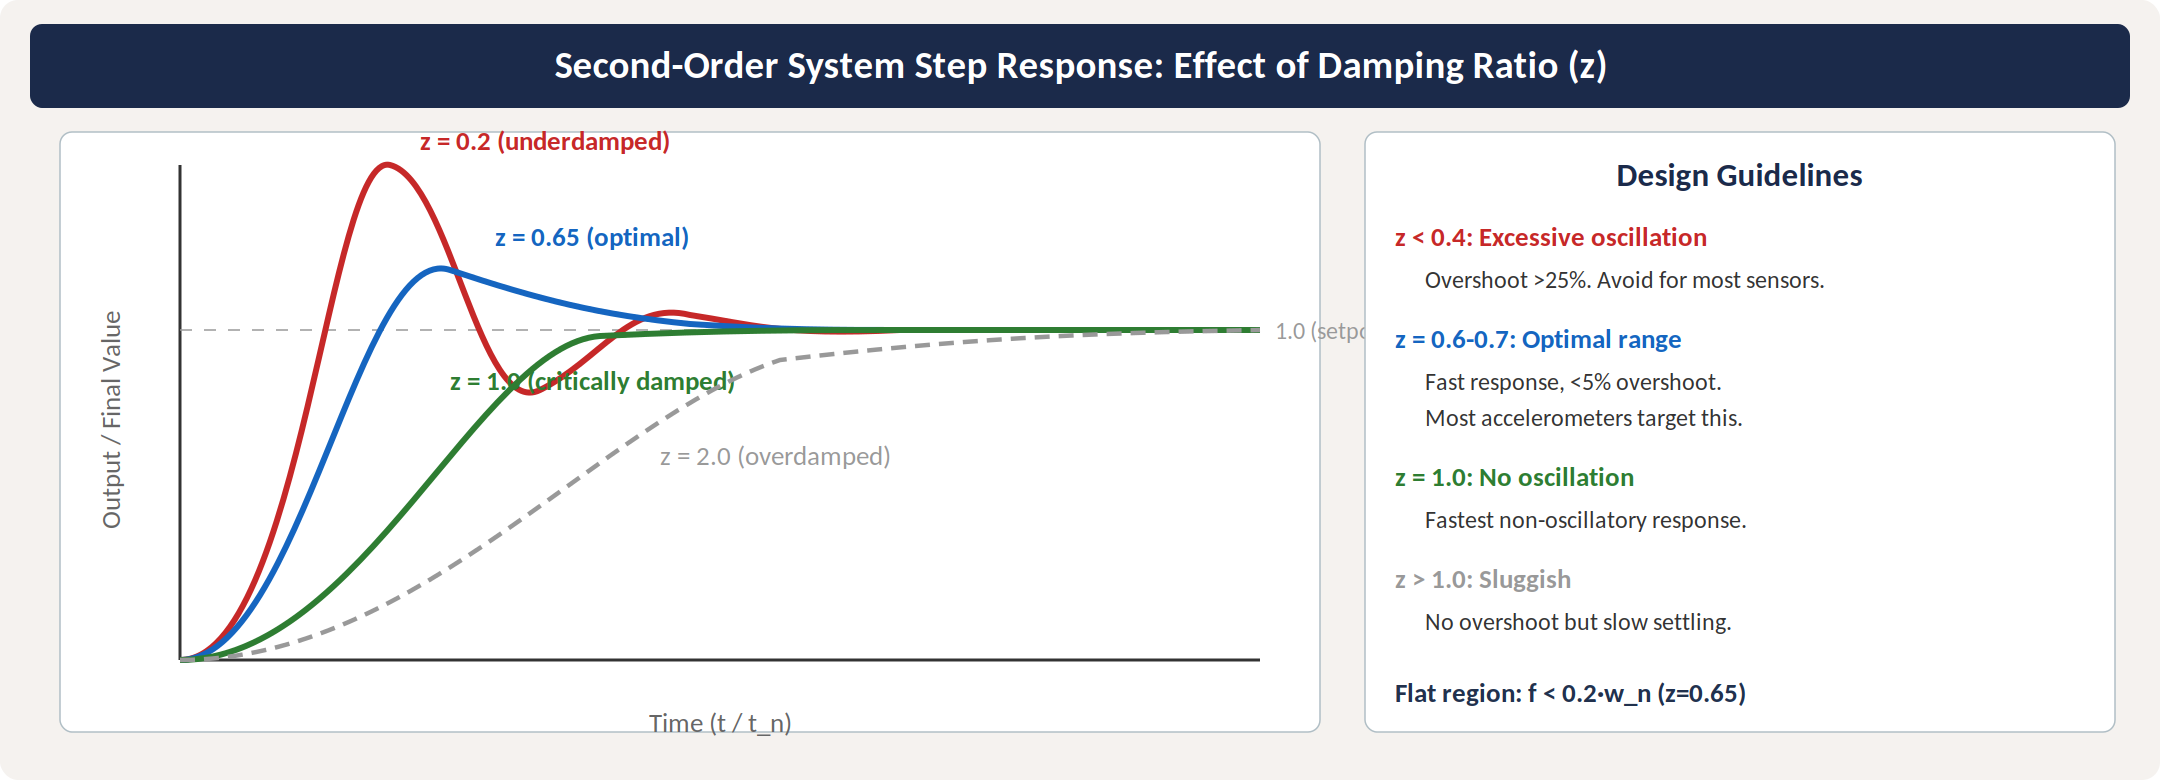
\includegraphics[width=\textwidth]{fig_second_order_response.png}
\caption{Second-order system step response for different damping ratios. The optimal range for most sensors is $\zeta = 0.6$--$0.7$, giving fast response with minimal overshoot.}
\label{fig:second_order}
\end{figure}

The sensor faithfully measures frequencies up to about $0.2\omega_n$ (flat within $\pm$5\% for $\zeta = 0.65$). Above $\omega_n$, the output rolls off at $-40$\,dB/decade.

\begin{tipbox}[The Rule of Five]
For a first-order sensor, allow $5\tau$ settling time for each measurement point. For a second-order sensor, use the signal frequency to less than $\omega_n / 5$ to stay in the flat region. Both rules give $<$1\% amplitude error.
\end{tipbox}

\section{Measuring Dynamic Characteristics}

\subsection{Step Test}
Apply a sudden step change in the measurand and record the sensor output vs.\ time. For a first-order sensor, plot $\ln(1 - y/y_{\infty})$ vs.\ $t$; the slope is $-1/\tau$. For a second-order sensor, measure the overshoot percentage ($M_p$) and peak time ($t_p$) to extract $\zeta$ and $\omega_n$:
\begin{equation}
\zeta = \frac{-\ln(M_p/100)}{\sqrt{\pi^2 + [\ln(M_p/100)]^2}}, \qquad \omega_n = \frac{\pi}{t_p \sqrt{1 - \zeta^2}}
\end{equation}

\subsection{Frequency Response Test}
Apply sinusoidal inputs at increasing frequencies and measure the output amplitude ratio and phase shift at each frequency. Plot the Bode diagram (magnitude in dB and phase in degrees vs.\ log frequency). This method is more thorough but requires a signal generator capable of producing sinusoidal variations in the measurand.


\section{Bandwidth and Rise Time}
Two related metrics describe how fast a sensor can respond:

\textbf{Bandwidth} ($f_{-3\text{dB}}$): the frequency at which the amplitude response drops to $-3$\,dB (70.7\% of the DC sensitivity). For a first-order system: $f_{-3\text{dB}} = 1/(2\pi\tau)$. For a second-order system: $f_{-3\text{dB}} \approx \omega_n / (2\pi)$ (exact value depends on $\zeta$).

\textbf{Rise time} ($t_r$): the time for the step response to go from 10\% to 90\% of the final value. For a first-order system: $t_r = 2.2\tau$. The approximate relationship between bandwidth and rise time:
\begin{equation}
f_{-3\text{dB}} \times t_r \approx 0.35
\end{equation}
This is a useful design rule: if you need to resolve events with a 1\,ms rise time, your sensor bandwidth must be $\geq$350\,Hz.

\section{Selecting a Sensor for Dynamic Measurements}
\begin{enumerate}[leftmargin=1.5em]
\item Identify the highest frequency of interest in the measurand ($f_{\max}$).
\item Select a sensor with $f_{-3\text{dB}} \geq 5 f_{\max}$ (to stay in the flat amplitude region with $<$1\% error).
\item Set the sampling rate $f_s \geq 10 f_{\max}$ (per Chapter~9) to capture the waveform shape.
\item Place an anti-aliasing filter at $f_c = 0.4 f_s$ before the ADC.
\end{enumerate}

\begin{keyconceptbox}[Requirements Mapping: Dynamic Response to Shall-Statements]
\begin{itemize}[nosep,leftmargin=1.5em]
\item ``Measure vibration up to 500\,Hz'' $\to$ SENS-REQ: Sensor bandwidth $\geq$2500\,Hz ($5\times$). DAQ-REQ: Sampling rate $\geq$5000\,S/s ($10\times$).
\item ``Resolve pressure transients with 0.5\,ms rise time'' $\to$ SENS-REQ: Sensor bandwidth $\geq$700\,Hz ($0.35/0.0005$). SENS-REQ: Sensor natural frequency $\geq$3500\,Hz ($5\times$ bandwidth).
\end{itemize}
\end{keyconceptbox}


\section{Why Dynamic Response Matters}
In static measurements, we wait for settling. In dynamic measurements, the measurand changes continuously and the sensor must track those changes. If the sensor cannot keep up, it attenuates and phase-shifts the signal, producing incorrect results.

\section{Zero-Order Systems}
Output instantaneously proportional to input: $y(t) = K \cdot x(t)$. A potentiometric sensor approximates this at low frequencies. No real sensor is truly zero-order; parasitic effects always introduce dynamics.

\section{First-Order Step Response in Depth}
For step input of magnitude $A$ at $t = 0$: $y(t) = KA(1 - e^{-t/\tau})$. At $\tau$: 63.2\%. At $2\tau$: 86.5\%. At $3\tau$: 95.0\%. At $5\tau$: 99.3\% (``settled''). If $\tau = 0.5$\,s, settling takes 2.5\,s.

\subsection{Frequency Response}
Magnitude: $|H| = 1/\sqrt{1+(\omega\tau)^2}$. Phase: $\phi = -\arctan(\omega\tau)$. At $f_{-3\text{dB}} = 1/(2\pi\tau)$: amplitude is 70.7\% (29\% error), phase is $-45^\circ$. For $<$5\% amplitude error: stay below $f_{-3\text{dB}}/3$. For $<$1\%: below $f_{-3\text{dB}}/7$.

\subsection{Measuring the Time Constant}
Apply step input (plunge thermocouple into hot water). Record output vs.\ time. Find time at 63.2\% of step change. That time is $\tau$. Alternatively: plot $\ln(1 - y/y_\infty)$ vs.\ $t$; slope is $-1/\tau$.

\begin{examplebox}[ThermoRig: Measuring Thermocouple Time Constant]
Plunge Type K TC from 23\,\degC{} air into 80\,\degC{} stirred water bath. At 100\,S/s, output reaches 63.2\% of 57\,\degC{} step (i.e., 59.0\,\degC{}) at $t = 0.42$\,s. Therefore $\tau = 0.42$\,s, $f_{-3\text{dB}} = 0.38$\,Hz. For signals up to 0.05\,Hz (convective heat transfer): amplitude error $<$1\%. For rapid thermal transients: too slow.
\end{examplebox}

\section{Second-Order Systems in Depth}
Governing equation: $(1/\omega_n^2)\ddot{y} + (2\zeta/\omega_n)\dot{y} + y = Kx(t)$.

\textbf{Underdamped ($\zeta < 1$)}: oscillates with decaying amplitude. Damped frequency $\omega_d = \omega_n\sqrt{1-\zeta^2}$. Overshoot: $\%OS = 100 \cdot e^{-\pi\zeta/\sqrt{1-\zeta^2}}$.

\textbf{Critically damped ($\zeta = 1$)}: fastest non-oscillatory approach.

\textbf{Overdamped ($\zeta > 1$)}: no oscillation but slower than critical.

\subsection{Frequency Response}
$|H| = 1/\sqrt{[1-(f/f_n)^2]^2 + [2\zeta(f/f_n)]^2}$. Usable flat band: $\sim 0.2 f_n$ for $\zeta = 0.65$, $\sim 0.4 f_n$ for $\zeta = 0.7$. This is why accelerometer datasheets specify a ``useful range'' that is a fraction of resonant frequency.

\subsection{The Bandwidth--Rise Time Tradeoff}
$B \times t_r \approx 0.35$ where $B$ is bandwidth (Hz) and $t_r$ is 10--90\% rise time (s). Faster sensor = wider bandwidth = more noise captured. Cannot independently improve both.

\begin{tipbox}[First vs.\ Second-Order Model Selection]
Smooth exponential step response with no overshoot $\to$ first-order. Overshoot and ringing $\to$ second-order. Thermal sensors are typically first-order. Mechanical sensors (accelerometers, pressure transducers) are second-order.
\end{tipbox}

\section{Practical Implications}
Rule 1: sensor bandwidth must exceed signal bandwidth by $5\times$ minimum ($10\times$ preferred). Rule 2: for transients, sensor rise time must be much shorter than event duration. Rule 3: in control systems, sensor phase lag directly affects stability margins.


\section{Time Domain vs.\ Frequency Domain Characterization}
Sensor dynamic behavior can be characterized in either domain. The step response (time domain) is intuitive: apply a sudden change and observe how the sensor responds. The frequency response (frequency domain) is more powerful for system design: it directly shows which frequencies the sensor can measure and which it attenuates.

The two representations are mathematically equivalent (connected by the Laplace transform), but each reveals different insights. Use the step response to evaluate settling time, overshoot, and rise time. Use the frequency response to evaluate bandwidth, resonance, and phase shift.

\section{Experimental Frequency Response Measurement}
To measure a sensor's frequency response experimentally: (1) Apply a sinusoidal input at frequency $f$. (2) Measure the input amplitude $A_{\text{in}}$ and output amplitude $A_{\text{out}}$. (3) Compute the gain: $|H(f)| = A_{\text{out}}/A_{\text{in}}$. (4) Measure the time delay $\Delta t$ between input and output peaks. (5) Compute the phase: $\phi = -360 \times f \times \Delta t$ degrees. (6) Repeat at 10--20 frequencies from $0.1 f_{-3\text{dB}}$ to $10 f_{-3\text{dB}}$, logarithmically spaced. (7) Plot the Bode diagram (gain in dB vs.\ log frequency; phase in degrees vs.\ log frequency).

For temperature sensors, generating a sinusoidal temperature input is difficult. Instead, use the step response method and extract the time constant. For mechanical sensors (accelerometers, pressure transducers), a shaker table provides calibrated sinusoidal acceleration at precise frequencies.

\section{Transfer Functions}
A transfer function $G(s) = Y(s)/X(s)$ describes the input-output relationship in the Laplace domain ($s = j\omega$).

First-order: $G(s) = K/(1 + \tau s)$. One pole at $s = -1/\tau$.

Second-order: $G(s) = K\omega_n^2/(s^2 + 2\zeta\omega_n s + \omega_n^2)$. Two poles at $s = -\zeta\omega_n \pm \omega_n\sqrt{\zeta^2 - 1}$.

The pole locations determine the dynamic behavior completely. Poles on the negative real axis produce exponential decay (first-order, overdamped). Complex conjugate poles produce oscillatory decay (underdamped). Poles on the imaginary axis produce sustained oscillation (critically stable). Poles on the positive real axis produce unstable (growing) response.

\section{Cascaded System Response}
When multiple dynamic elements are in series (sensor $\to$ amplifier $\to$ filter), the overall transfer function is the product of individual transfer functions: $G_{\text{total}}(s) = G_1(s) \cdot G_2(s) \cdot G_3(s)$. In the frequency domain, magnitudes multiply (or add in dB) and phases add.

Example: a thermocouple ($\tau = 0.5$\,s, $f_{-3\text{dB}} = 0.32$\,Hz) followed by a 2nd-order Butterworth filter at 10\,Hz. At 0.1\,Hz: thermocouple gain is $-0.4$\,dB, filter gain is $-0.0$\,dB; total is $-0.4$\,dB (acceptable). At 1\,Hz: thermocouple is $-10$\,dB (the sensor, not the filter, limits performance). The system bandwidth is determined by the slowest element.

\begin{examplebox}[ThermoRig: Cascaded Dynamic Response]
The ThermoRig signal chain dynamic response: thermocouple ($\tau = 0.42$\,s, $f_{-3\text{dB}} = 0.38$\,Hz) $\to$ INA128 ($f_{-3\text{dB}} \approx 1.6$\,kHz at $G = 611$, negligible lag at signal frequencies) $\to$ Sallen-Key LP ($f_c = 40$\,Hz, 2nd order, negligible lag below 4\,Hz). The overall system bandwidth is limited entirely by the thermocouple at 0.38\,Hz. The amplifier and filter contribute less than 0.01\,dB of attenuation and less than 0.1$^\circ$ of phase shift at frequencies below 1\,Hz. This is typical: in thermal measurement systems, the sensor dynamics dominate.
\end{examplebox}

\section{Sensor Dynamic Compensation}
If the sensor's dynamic response is too slow for the measurement, mathematical compensation can partially recover the attenuated high-frequency content. For a first-order sensor with known $\tau$:
\begin{equation}
x_{\text{true}}(t) \approx y(t) + \tau \frac{dy}{dt}
\end{equation}
where $y(t)$ is the measured output and $x_{\text{true}}(t)$ is the estimated true input. In the frequency domain, this is an inverse filter: multiply the measured spectrum by $1 + j\omega\tau$ (the inverse of the sensor's transfer function).

Caution: dynamic compensation amplifies high-frequency noise (the derivative term). It is only practical when the sensor's bandwidth is within a factor of 2--5 of the signal bandwidth, and when the SNR at high frequencies is adequate. Beyond this, the noise amplification overwhelms the recovered signal.

\section{Aliasing from Sensor Dynamics}
A sensor acts as a low-pass filter. If the sensor bandwidth is less than $f_s/2$, it provides inherent anti-alias filtering. However, this is not deliberate and should not be relied upon. The sensor's rolloff may not be steep enough (first-order: only $-20$\,dB/decade), and the exact bandwidth may vary with operating conditions (temperature, mounting). Always include a dedicated anti-alias filter in the signal chain.
\section{Measuring Sensor Time Constants: Advanced Methods}
\subsection{Plunge Test Details}
For thermal sensors, the plunge test is the gold standard. Critical details: (1)~the fluid must be well-stirred to eliminate thermal boundary layers (use a magnetic stirrer or continuous manual agitation), (2)~the fluid temperature must be uniform and known (use a calibrated reference thermometer), (3)~the initial sensor temperature must be stable (allow 5 minutes of equilibration before plunging), (4)~the data acquisition rate must be fast enough to capture the transient ($f_s \geq 10/\tau$; for $\tau = 0.5$\,s: $f_s \geq 20$\,S/s), (5)~compute $\tau$ using the 63.2\% method \emph{and} the log-linear fit method, and compare. If they agree within 5\%, the first-order model is valid.

\subsection{Sinusoidal Testing}
For sensors where a sinusoidal input is practical (vibration shakers for accelerometers, modulated light sources for photodetectors), sweep the input frequency from $0.1 f_{-3\text{dB}}$ to $10 f_{-3\text{dB}}$ in 20+ steps. At each frequency, measure the gain $|H| = A_{\text{out}}/A_{\text{in}}$ and the phase lag. The Bode plot provides the complete dynamic characterization, including the order of the system and any resonance behavior.

\section{Higher-Order System Dynamics}
Some sensors exhibit dynamics that are neither purely first-order nor second-order. A thermocouple welded to a heavy metal block may show a fast initial response (the junction itself, $\tau_1 \approx 0.1$\,s) followed by a slow drift to final value (the block equilibrating, $\tau_2 \approx 30$\,s). This is a two-time-constant system:
\begin{equation}
G(s) = \frac{K}{(1 + \tau_1 s)(1 + \tau_2 s)}
\end{equation}
The step response shows a fast initial rise followed by a slow creep. The dominant (larger) time constant determines the settling time; the faster time constant determines the initial response rate. In the frequency domain, there are two breakpoints on the Bode plot.

\section{Sensor Bandwidth and Control System Interaction}
In a feedback control system, the sensor is part of the loop. Its dynamic response affects stability. A sensor with time constant $\tau_s$ introduces phase lag $\phi = -\arctan(\omega \tau_s)$ at the crossover frequency. If this lag reduces the total phase margin below 45\degC{}, the system becomes oscillatory or unstable.

Rule of thumb: the sensor bandwidth must be at least $5\times$ the closed-loop bandwidth. For a control system with 0.1\,Hz bandwidth (10\,s settling time): sensor $f_{-3\text{dB}} \geq 0.5$\,Hz ($\tau \leq 0.32$\,s). The ThermoRig thermocouple ($\tau = 0.42$\,s, $f_{-3\text{dB}} = 0.38$\,Hz) is marginally adequate; a faster thermocouple or an exposed-junction design would provide more stability margin.
\section{Amplitude Ratio and Phase Measurement}
When characterizing sensor dynamics experimentally, two quantities must be measured at each test frequency: the amplitude ratio $M(\omega) = |Y|/(K|X|)$ and the phase angle $\phi(\omega)$.

For amplitude ratio: apply a sinusoidal input of known amplitude $A_{\text{in}}$ at frequency $f$. Measure the output amplitude $A_{\text{out}}$ after the transient has decayed (wait at least $5\tau$ or 10 cycles, whichever is longer). The amplitude ratio is $M = A_{\text{out}}/(K \cdot A_{\text{in}})$ where $K$ is the static sensitivity.

For phase angle: measure the time delay $\Delta t$ between the input and output waveforms (zero-crossing to zero-crossing, or peak to peak). The phase angle in degrees is $\phi = -360 \cdot f \cdot \Delta t$. For a first-order system, $\phi$ is always negative (output lags input) and ranges from 0\,\degC{} at DC to $-90$\,\degC{} at infinite frequency. For a second-order system, $\phi$ ranges from 0\,\degC{} to $-180$\,\degC{}, passing through $-90$\,\degC{} at the natural frequency.

\section{Practical Impact of Sensor Dynamics: Worked Examples}
\textbf{Example 1: Temperature measurement during soldering.} A solder joint reaches peak temperature in approximately 2\,s. A thermocouple with $\tau = 0.5$\,s reads only 86\% of the peak temperature at $t = 2$\,s (missing $\sim$40\,\degC{} if the peak is 280\,\degC{}). A thermocouple with $\tau = 0.05$\,s (exposed junction, 0.25\,mm wire) reads 99.95\% of the peak. For process control where the peak temperature must not exceed 290\,\degC{}, the slow thermocouple could allow a 40\,\degC{} overshoot without detection.

\textbf{Example 2: Pressure measurement in a hydraulic actuator.} The pressure oscillates at 50\,Hz due to pump ripple. A pressure transducer with $f_n = 500$\,Hz ($\zeta = 0.7$) has an amplitude ratio of $M = 1/\sqrt{(1-0.01)^2 + (0.14)^2} = 1.005$ at 50\,Hz, practically perfect. A cheaper transducer with $f_n = 100$\,Hz ($\zeta = 0.4$) has $M = 1/\sqrt{(1-0.25)^2 + (0.4)^2} = 1.21$ at 50\,Hz, overstating the pressure by 21\%. At 80\,Hz, the resonance amplification makes the reading meaningless.

\textbf{Example 3: Vibration measurement on a rotating shaft.} An accelerometer with $f_n = 25$\,kHz ($\zeta = 0.7$) has a flat response ($\pm$5\%) up to approximately $0.2 \times 25000 = 5000$\,Hz. If the shaft rotates at 3600\,RPM (60\,Hz), harmonics up to the 80th (4800\,Hz) are measured accurately. A cheaper accelerometer with $f_n = 5$\,kHz is flat only to 1000\,Hz, measuring only the first 16 harmonics.

\section{White Noise Testing for System Identification}
Instead of sweeping individual frequencies, apply broadband white noise as the input and compute the frequency response function using cross-spectral analysis (Chapter~8). This characterizes the entire frequency response in a single measurement. The coherence function $\gamma^2(f)$ at each frequency indicates the quality of the measurement: $\gamma^2 > 0.95$ means the estimate is reliable; $\gamma^2 < 0.5$ means the SNR at that frequency is too low.

For thermal systems where white noise temperature input is impractical, use a Pseudo-Random Binary Sequence (PRBS): a square wave that switches between two temperatures at random intervals. The PRBS has a flat spectrum up to a frequency determined by the minimum switching interval, effectively exciting all frequencies simultaneously.
\section{System Identification from Experimental Data}
Determining the dynamic model (transfer function) of a sensor or plant from measured data is called \textbf{system identification}. For MEGN~300 applications, two simple methods suffice:

\subsection{Step Response Method}
Apply a step input and record the output. For a first-order system: (1) measure the final steady-state value $y_{ss}$, (2) measure the time to reach $0.632 y_{ss}$ to get $\tau$, (3) the transfer function is $G(s) = y_{ss}/(1 + \tau s)$. For a second-order system: (1) measure the peak overshoot $\%OS$ to determine $\zeta$: $\zeta = -\ln(\%OS/100)/\sqrt{\pi^2 + \ln^2(\%OS/100)}$, (2) measure the peak time $t_p$ to determine $\omega_d$: $\omega_d = \pi/t_p$, (3) compute $\omega_n = \omega_d/\sqrt{1-\zeta^2}$, (4) the transfer function is $G(s) = K\omega_n^2/(s^2 + 2\zeta\omega_n s + \omega_n^2)$.

\subsection{Frequency Response Method}
Sweep a sinusoidal input across a range of frequencies. At each frequency, measure the gain $|H| = A_{\text{out}}/A_{\text{in}}$ and the phase $\phi$. Plot the Bode diagram. For a first-order system: the $-3$\,dB frequency gives $\tau = 1/(2\pi f_{-3\text{dB}})$. For a second-order system: the resonant peak frequency and height give $\omega_n$ and $\zeta$.

The frequency response method is more accurate than the step response method for second-order systems because it provides data at many frequencies, allowing curve fitting to reduce the effect of noise. However, it requires a sinusoidal input source, which is easy for electrical and mechanical systems but difficult for thermal systems.

\section{Dynamic Range of Sensor Systems}
The dynamic range of a sensor is the ratio between its maximum measurable input and its minimum resolvable input, both determined by dynamic characteristics:

\textbf{Upper limit}: determined by the sensor's linear range. Beyond this, the output saturates or becomes nonlinear. For an accelerometer with $\pm$50\,g range: the maximum input is 50\,g.

\textbf{Lower limit}: determined by the noise floor. For the same accelerometer with a noise floor of 100\,$\mu$g/$\sqrt{\text{Hz}}$ and a 1\,kHz bandwidth: the minimum resolvable acceleration is $100 \times \sqrt{1000} = 3.16$\,mg $\approx 3$\,mg.

\textbf{Dynamic range}: $20\log_{10}(50/0.003) = 84$\,dB ($\sim$14 bits equivalent). The DAQ must have at least this dynamic range to utilize the sensor's full capability. A 12-bit ADC (72\,dB) would limit the usable range; a 16-bit ADC (96\,dB) provides headroom.

\section{Anti-Resonance and Its Effects}
Some measurement systems exhibit \textbf{anti-resonance}: a frequency at which the sensor output drops to near zero, even though the input is non-zero. Anti-resonance occurs when two parallel signal paths with different phase produce destructive interference. In vibration measurement, a mounting structure with internal resonances can create anti-resonances in the accelerometer's frequency response, producing ``blind spots'' where vibration at specific frequencies is invisible. The cure: verify the complete frequency response of the installed sensor (not just the sensor alone) and avoid measurements at anti-resonance frequencies.
\section{Practice Questions}
\begin{enumerate}[leftmargin=1.5em]
\item A temperature sensor has $\tau = 3.0$\,s. How long must you wait after a step change for the reading to be within 1\% of the true value?
\item A first-order pressure sensor ($\tau = 0.5$\,ms) measures a pressure signal oscillating at 500\,Hz. Calculate the amplitude attenuation (as a percentage of true amplitude) and the phase lag in degrees.
\item An accelerometer step response shows 15\% overshoot and a peak time of 2.0\,ms. Calculate $\zeta$ and $\omega_n$.
\item Your system must measure a vibration signal containing frequencies up to 200\,Hz with less than 5\% amplitude error. What minimum natural frequency must your accelerometer have if $\zeta = 0.65$?
\item Explain why wrapping a thermocouple in thermal paste improves its dynamic response when measuring surface temperature, even though the paste itself has low thermal conductivity.
\end{enumerate}

\subsection{Answers}
\begin{enumerate}[leftmargin=1.5em]
\item Within 1\% means $e^{-t/\tau} < 0.01$, so $t > -\tau \ln(0.01) = 3.0 \times 4.605 = 13.8$\,s (i.e., $4.6\tau$; often rounded to $5\tau = 15$\,s).
\item $\omega = 2\pi \times 500 = 3142$\,rad/s. $\omega\tau = 3142 \times 0.0005 = 1.571$. $M = 1/\sqrt{1 + 1.571^2} = 1/\sqrt{3.468} = 0.537$. Amplitude = 53.7\% of true (attenuated by 46.3\%). Phase $= -\arctan(1.571) = -57.5$\ang{}.
\item $\zeta = -\ln(0.15)/\sqrt{\pi^2 + [\ln(0.15)]^2} = 1.897/\sqrt{9.870 + 3.599} = 1.897/3.669 = 0.517$. $\omega_n = \pi/(0.002 \times \sqrt{1 - 0.267}) = \pi/(0.002 \times 0.856) = 1835$\,rad/s = 292\,Hz.
\item For $\zeta = 0.65$, the flat region extends to $\approx 0.2\omega_n$ for $<$5\% error. So $0.2\omega_n \geq 2\pi \times 200$, giving $\omega_n \geq 6283$\,rad/s $= 1000$\,Hz. The accelerometer's natural frequency must be at least 1000\,Hz.
\item Thermal paste fills the microscopic air gaps between the thermocouple bead and the surface. Air has very low thermal conductivity ($\sim$0.025\,W/m$\cdot$K), so air gaps create a large thermal resistance that increases the effective time constant. The paste ($\sim$1--5\,W/m$\cdot$K) dramatically reduces this contact resistance, lowering $\tau$ and improving dynamic response, even though the paste itself is not a great conductor compared to metal.
\end{enumerate}


% ================================================================
\chapter{Error Analysis and Uncertainty}

\section{Types of Error}

\subsection{Systematic Error (Bias)}
Systematic errors shift all measurements in one direction by a consistent amount. They arise from calibration errors, environmental effects (temperature, humidity), sensor nonlinearity, loading effects, and installation errors. Systematic errors are \textbf{correctable} through calibration, environmental compensation, and improved technique. They do \textbf{not} decrease with repeated measurements.

\subsection{Random Error (Precision Error)}
Random errors cause scatter around the mean value due to inherent variability in the measurement process (electronic noise, vibration, turbulence, human reading variation). Random errors follow a statistical distribution (usually Gaussian) and \textbf{decrease with averaging}: the standard error of the mean $= \sigma / \sqrt{n}$.

\subsection{Gross Errors (Blunders)}
Mistakes: wrong wiring, reading the wrong scale, recording errors, equipment malfunction. Detected and eliminated by inspection, redundancy, and outlier analysis (Chauvenet's criterion or Grubbs' test).

\begin{warningbox}[You Cannot Average Away Systematic Error]
If your thermometer reads 2\,\degC{} high due to a calibration offset, taking 1000 measurements and averaging them will give you a very precise number that is still 2\,\degC{} wrong. Calibrate first, then average.
\end{warningbox}

\section{Statistical Foundations}

\subsection{Mean, Standard Deviation, and Standard Error}
For $n$ measurements $\{x_1, x_2, \ldots, x_n\}$:
\begin{align}
\bar{x} &= \frac{1}{n} \sum_{i=1}^{n} x_i \quad \text{(sample mean)} \\
s &= \sqrt{\frac{1}{n-1} \sum_{i=1}^{n} (x_i - \bar{x})^2} \quad \text{(sample standard deviation)} \\
s_{\bar{x}} &= \frac{s}{\sqrt{n}} \quad \text{(standard error of the mean)}
\end{align}
Use $n-1$ (Bessel's correction) in the denominator for sample standard deviation. The standard error quantifies the uncertainty of the mean itself; the standard deviation quantifies the spread of individual measurements.

\subsection{Confidence Intervals}
The true value lies within $\bar{x} \pm t_{\nu,P} \cdot s_{\bar{x}}$ with probability $P$, where $t_{\nu,P}$ is the Student's $t$-value for $\nu = n-1$ degrees of freedom at confidence level $P$.

Common values: for 95\% confidence and large $n$: $t \approx 2.0$. For $n = 5$: $t_{4,95\%} = 2.776$. For $n = 10$: $t_{9,95\%} = 2.262$.

\begin{tipbox}[Report Uncertainty Correctly]
Always report measurements as: $\bar{x} \pm U$ (95\% confidence, $n$ = [sample size]). For example: ``$T = 25.3 \pm 0.4$\,\degC{} (95\% CI, $n = 10$).'' This gives the reader everything needed to evaluate the quality of your measurement.
\end{tipbox}

\section{Uncertainty Propagation}

When a result $R$ is calculated from measured quantities $x_1, x_2, \ldots, x_n$:
\begin{equation}
R = f(x_1, x_2, \ldots, x_n)
\end{equation}
the uncertainty in $R$ propagates from the uncertainties in each $x_i$:
\begin{equation}
u_R = \sqrt{\sum_{i=1}^{n} \left(\frac{\partial f}{\partial x_i}\right)^2 u_{x_i}^2}
\end{equation}
This is the \textbf{RSS (root-sum-square)} method, valid when the $x_i$ errors are independent and random.

\subsection{Special Cases}
\textbf{Addition/Subtraction}: $R = x_1 \pm x_2 \Rightarrow u_R = \sqrt{u_{x_1}^2 + u_{x_2}^2}$.

\textbf{Multiplication/Division}: $R = x_1 \cdot x_2 / x_3 \Rightarrow u_R/R = \sqrt{(u_{x_1}/x_1)^2 + (u_{x_2}/x_2)^2 + (u_{x_3}/x_3)^2}$.

\textbf{Power}: $R = x^n \Rightarrow u_R/R = |n| \cdot u_x / x$.

\begin{examplebox}[ThermoRig: Uncertainty Propagation for Heat Flux]
Heat flux through a wall: $q = k \cdot \Delta T / L$, where $k = 0.50 \pm 0.02$\,W/(m$\cdot$K), $\Delta T = 20.0 \pm 0.8$\,\degC{}, $L = 0.010 \pm 0.0005$\,m.
\[
\frac{u_q}{q} = \sqrt{\left(\frac{0.02}{0.50}\right)^2 + \left(\frac{0.8}{20.0}\right)^2 + \left(\frac{0.0005}{0.010}\right)^2} = \sqrt{0.0016 + 0.0016 + 0.0025} = 0.0755 = 7.55\%
\]
$q = 0.50 \times 20.0 / 0.010 = 1000$\,W/m$^2$. $u_q = 75.5$\,W/m$^2$. Report: $q = 1000 \pm 76$\,W/m$^2$.

The thickness measurement ($L$) dominates the uncertainty. To improve the result, improve the length measurement first.
\end{examplebox}

\section{Design-Stage Uncertainty Estimation}

Before building a measurement system, estimate the total uncertainty from manufacturer specifications:

\begin{enumerate}[leftmargin=1.5em]
\item List all error sources in the measurement chain (sensor accuracy, signal conditioning gain error, ADC quantization, noise).
\item Convert each to the same units (typically the measurand's engineering units).
\item Classify each as systematic (bias) or random.
\item RSS the random components. Add the worst-case systematic components algebraically.
\item Compare to the measurement requirement. If the total exceeds the requirement, identify the dominant contributor and improve it.
\end{enumerate}

\begin{figure}[htbp]
\centering
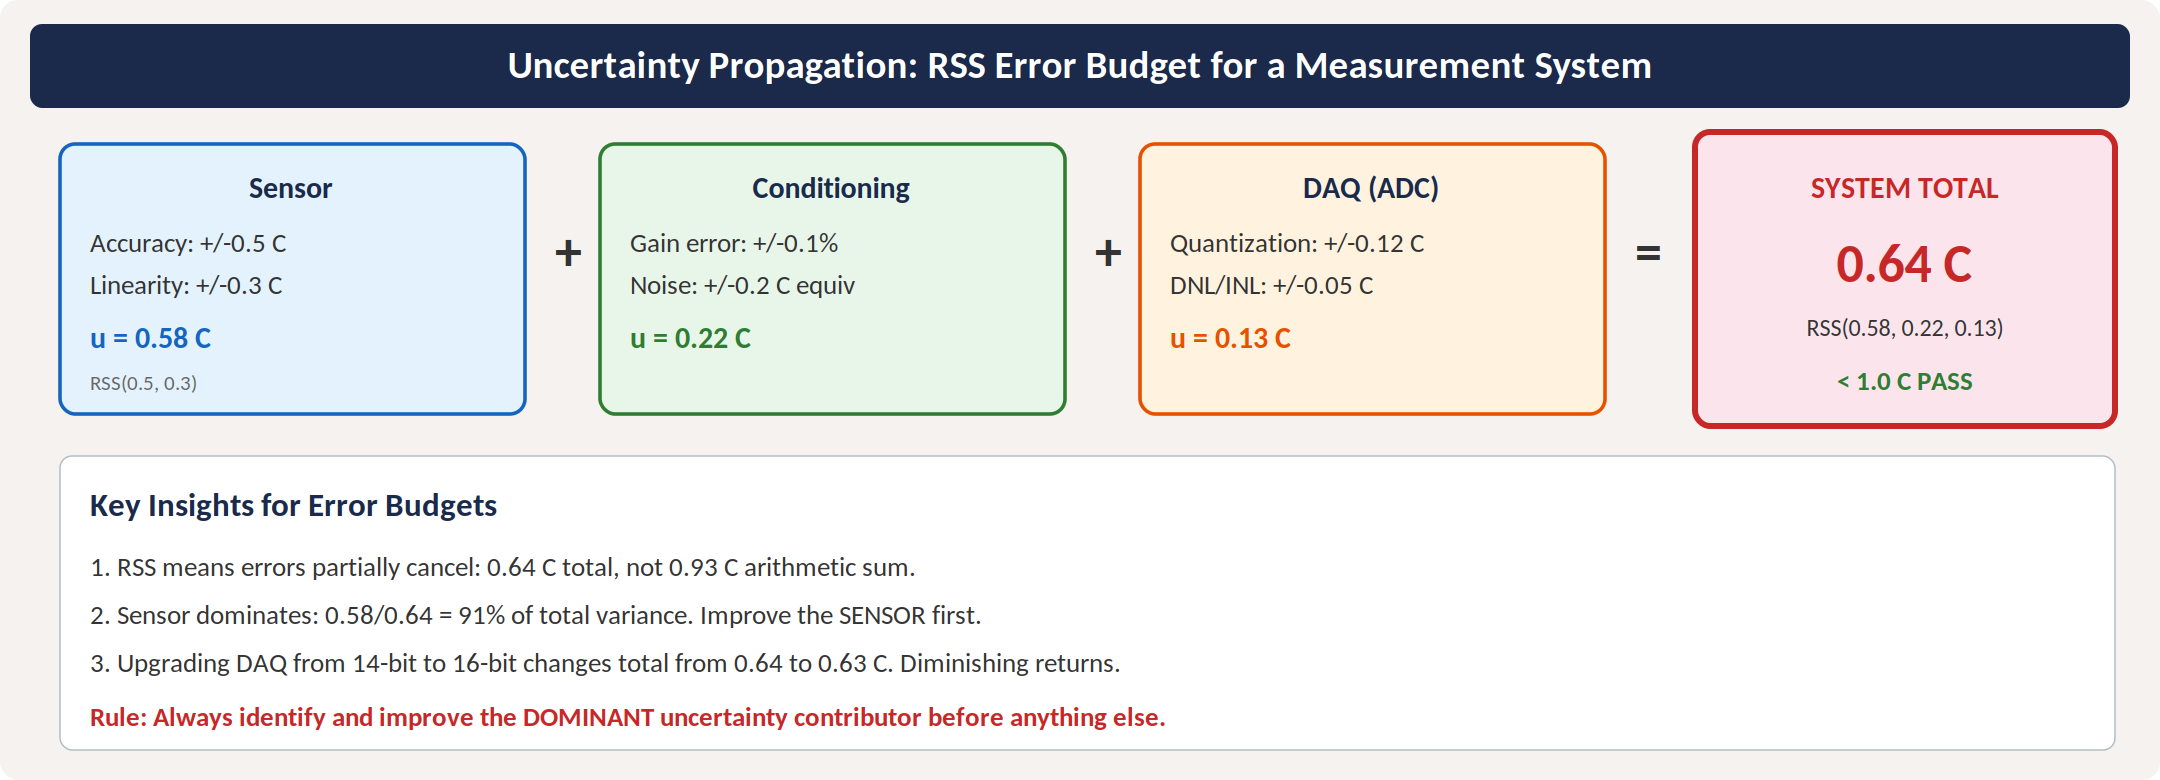
\includegraphics[width=\textwidth]{fig_error_budget.png}
\caption{RSS error budget for a temperature measurement system. The sensor dominates the total uncertainty; improving the ADC has diminishing returns. Always improve the dominant contributor first.}
\label{fig:error_budget}
\end{figure}

\begin{keyconceptbox}[Requirements Mapping: Uncertainty to Shall-Statements]
\begin{itemize}[nosep,leftmargin=1.5em]
\item ``Measure temperature to $\pm$1.0\,\degC{} at 95\% confidence'' $\to$ MEAS-REQ: Total expanded uncertainty $U_{95} \leq 1.0$\,\degC{}, verified by calibration against a NIST-traceable standard.
\item The error budget allocates this across the sensor, conditioning, and DAQ stages. Each stage becomes a subsystem requirement.
\end{itemize}
\end{keyconceptbox}


\section{The Philosophy of Uncertainty}
Every measured value is an estimate accompanied by a range within which the true value is believed to lie. A reading of ``23.5\,\degC{}'' is meaningless without knowing whether the uncertainty is $\pm$0.1\,\degC{} or $\pm$5\,\degC{}.

\section{Type A and Type B Evaluation}
\textbf{Type A (statistical)}: from repeated measurements. Standard uncertainty of the mean: $u_A = s/\sqrt{N}$. As $N$ increases, $u_A$ decreases (but doubling $N$ only reduces by $\sqrt{2}$).

\textbf{Type B (non-statistical)}: from datasheets, calibration certificates, engineering judgment. For $\pm a$ specification with rectangular distribution: $u_B = a/\sqrt{3}$. Normal distribution (95\%): $u_B = a/2$.

\section{Combined Standard Uncertainty (RSS)}
For $R = f(x_1, x_2, \ldots)$:
\begin{equation}
u_c(R) = \sqrt{\sum_{i}\left(\frac{\partial f}{\partial x_i}\right)^2 u^2(x_i)}
\end{equation}
Each $(\partial f/\partial x_i)^2 u^2(x_i)$ is a variance contribution. The partial derivative is the sensitivity coefficient.

\textbf{Sums/differences}: $u_c = \sqrt{u_1^2 + u_2^2}$. \textbf{Products/quotients}: relative uncertainties add in quadrature. \textbf{Powers} $R = x^n$: $u_c/R = |n| \cdot u_x/x$. Velocity uncertainty of 5\% means kinetic energy uncertainty of 10\%.

\begin{examplebox}[ThermoRig: Uncertainty in Heat Flux]
$q = k \Delta T / L$. Given: $k = 1.05 \pm 0.03$\,W/mK, $T_1 = 80.2 \pm 0.4$\,\degC{}, $T_2 = 23.1 \pm 0.4$\,\degC{}, $L = 0.0100 \pm 0.0002$\,m.

$\Delta T = 57.1$\,\degC{}, $u_{\Delta T} = \sqrt{0.4^2+0.4^2} = 0.566$\,\degC{}. $q = 5995.5$\,W/m$^2$.

Relative: $u_k/k = 2.86\%$, $u_{\Delta T}/\Delta T = 0.99\%$, $u_L/L = 2.00\%$.

$u_q/q = \sqrt{2.86^2+0.99^2+2.00^2}\% = 3.63\%$. $u_q = 218$\,W/m$^2$.

Result: $q = 6000 \pm 220$\,W/m$^2$. Thermal conductivity dominates (62\% of variance).
\end{examplebox}

\section{Expanded Uncertainty and Confidence Intervals}
$U = k \cdot u_c$. Coverage factor $k = 2$ for 95\% confidence (standard in engineering), $k = 3$ for 99.7\%. Always report: ``$T = 23.5 \pm 0.8$\,\degC{} ($k = 2$).'' For small samples ($N < 30$), use Student's $t$-distribution with Welch-Satterthwaite effective degrees of freedom.

\section{Systematic Error Sources and Corrections}
\textbf{Sensor bias}: calibrate and apply correction. \textbf{Environmental effects}: characterize sensitivity coefficients. \textbf{Loading effects}: use higher-impedance instruments (Ch.\ 1). \textbf{Operator bias}: use digital readout. \textbf{Algorithmic bias}: use double-precision throughout.

\begin{warningbox}[Accuracy vs.\ Precision]
Accuracy $=$ total uncertainty (systematic + random). Precision $=$ repeatability (random only). Precision is always better than accuracy. After calibration, accuracy improves toward precision but never exceeds it. Datasheet ``accuracy: $\pm$1\%'' $\neq$ ``repeatability: $\pm$0.1\%.''
\end{warningbox}

\section{Designing the Error Budget}
(1) Start with system requirement. (2) Identify all sources. (3) Estimate each from datasheets/calibration. (4) Compute RSS total. (5) Verify meets requirement. (6) If not, improve the dominant contributor.

The dominant contributor determines the total. A 10\% improvement in the largest source has more impact than 50\% improvement in all minor sources combined.

\begin{tipbox}[The 80/20 Rule]
In most systems, 80\% of total uncertainty comes from one or two sources. Find them first. Display the error budget as a pie chart of variance contributions; the largest slice is where you invest effort.
\end{tipbox}

\section{Reporting Measurements}
Never report more significant figures than the uncertainty justifies. If uncertainty is $\pm$0.5\,\degC{}, report ``23.5 $\pm$ 0.5\,\degC{},'' not ``23.472\,\degC{}.'' Match decimal places in value and uncertainty.


\section{Monte Carlo Uncertainty Analysis}
When the measurement equation is complex (nonlinear, conditional, or involves lookup tables), the analytical RSS formula becomes difficult or impossible to apply. Monte Carlo simulation provides a general alternative:

(1) Assign a probability distribution to each input variable (normal, rectangular, triangular, etc.) based on the available uncertainty information. (2) Generate $N$ random samples of each input ($N \geq 10{,}000$). (3) For each set of input samples, compute the output using the measurement equation. (4) Analyze the distribution of the $N$ output values: mean, standard deviation, percentiles.

The 2.5th and 97.5th percentiles of the output distribution provide the 95\% coverage interval directly, without assuming a normal distribution. This is especially valuable when the output distribution is asymmetric (which can occur with nonlinear measurement equations).

\begin{examplebox}[ThermoRig: Monte Carlo vs.\ RSS for Heat Flux]
For the heat flux calculation $q = k\Delta T/L$, we compare analytical RSS and Monte Carlo results. RSS (from the earlier example): $q = 6000 \pm 218$\,W/m$^2$ (3.6\%). Monte Carlo ($N = 100{,}000$, all inputs normal): mean $= 5998$\,W/m$^2$, std $= 215$\,W/m$^2$, 95\% interval $= [5577, 6428]$\,W/m$^2$. The agreement is excellent because the measurement equation is approximately linear over the uncertainty ranges. For this problem, the simpler RSS method is adequate. Monte Carlo becomes essential for equations involving powers, exponentials, or conditional logic.
\end{examplebox}

\section{Correlation Between Inputs}
The RSS formula assumes all input uncertainties are independent (uncorrelated). If two inputs are correlated (e.g., two temperatures measured by the same type of sensor, which share the same calibration bias), the combined uncertainty must include cross-terms:
\begin{equation}
u_c^2 = \sum_i c_i^2 u_i^2 + 2\sum_{i<j} c_i c_j u_i u_j r_{ij}
\end{equation}
where $r_{ij}$ is the correlation coefficient ($-1 \leq r_{ij} \leq 1$). Positive correlation ($r > 0$) increases the combined uncertainty; negative correlation ($r < 0$) decreases it. In the ThermoRig, $T_1$ and $T_2$ are measured by different thermocouples, so they are independent ($r = 0$). If they shared one thermocouple (e.g., measuring the same point at different times), they would be correlated.

\section{Degrees of Freedom and Student's t-Distribution}
When the number of measurements is small ($N < 30$), the normal distribution underestimates the uncertainty. The Student's $t$-distribution, which has heavier tails, provides more conservative (and more accurate) coverage intervals.

For $N$ measurements, the degrees of freedom $\nu = N - 1$. The coverage factor for 95\% confidence: $k = t_{0.975, \nu}$. For $N = 5$: $k = 2.78$ (vs.\ 2.00 for normal). For $N = 10$: $k = 2.26$. For $N = 30$: $k = 2.04$ (approaching the normal value). This is why small sample sizes produce wider confidence intervals: there is less statistical evidence for the true mean and standard deviation.

\section{Systematic Error Discovery}
Systematic errors are insidious because they affect every measurement consistently but invisibly. Techniques for discovering them:

\textbf{Comparison with independent methods}: measure the same quantity with two fundamentally different sensors (e.g., thermocouple and RTD, or optical and contact displacement). If the results disagree beyond the combined uncertainty, at least one has a systematic error.

\textbf{Swap test}: interchange two sensors (swap channel connections). If the discrepancy follows the sensor, it is a sensor bias. If it follows the channel, it is a DAQ or wiring error.

\textbf{Substitution test}: replace the sensor with a known reference signal (precision voltage source). Compare the DAQ reading to the known value. Any difference is a systematic error in the signal conditioning or DAQ chain.

\textbf{Reversal test}: for sensors with a directional property (strain gauges, force sensors), reverse the direction of the measurand. The average of forward and reverse readings cancels hysteresis and reveals the true zero.

\section{Uncertainty in Derived Quantities}
Many engineering measurements compute a derived quantity from multiple measured inputs. Examples:

\textbf{Flow rate} from differential pressure: $Q = C_d A \sqrt{2\Delta P/\rho}$. The square root means that $u_Q/Q = 0.5 \times u_{\Delta P}/\Delta P$. Flow measurement uncertainty is half the pressure measurement uncertainty (a favorable leverage).

\textbf{Power} from voltage and current: $P = VI$. Relative uncertainty: $u_P/P = \sqrt{(u_V/V)^2 + (u_I/I)^2}$.

\textbf{Efficiency}: $\eta = P_{\text{out}}/P_{\text{in}}$. Since this is a ratio, relative uncertainties add in quadrature. A system with 3\% uncertainty in both input and output power has $\sqrt{3^2 + 3^2} = 4.2\%$ uncertainty in efficiency.

\textbf{Strain from bridge voltage}: $\epsilon = (4V_o)/(V_{ex} \cdot GF)$. Three uncertainty sources multiply: excitation voltage, gauge factor, and output voltage. A 0.1\% excitation uncertainty, 1\% gauge factor uncertainty, and 0.5\% voltage measurement uncertainty give $\sqrt{0.1^2 + 1.0^2 + 0.5^2} = 1.1\%$ strain uncertainty. The gauge factor dominates.
\section{Uncertainty in Curve-Fit Calibrations}
When a calibration curve is fitted to data points, the calibration uncertainty includes: (1)~the uncertainty of each reference point (from the reference standard), (2)~the scatter of repeated measurements at each point (Type A), (3)~the fit residuals (difference between data and fitted curve), and (4)~the interpolation uncertainty (between calibration points).

For a linear fit $y = mx + b$ to $N$ calibration points: the uncertainty of a predicted value $\hat{y}$ at input $x_0$ is:
\begin{equation}
u(\hat{y}) = s_{\text{resid}} \sqrt{\frac{1}{N} + \frac{(x_0 - \bar{x})^2}{\sum(x_i - \bar{x})^2}}
\end{equation}
where $s_{\text{resid}} = \sqrt{\sum(y_i - \hat{y}_i)^2/(N-2)}$ is the residual standard error. The uncertainty is smallest at the center of the calibration range ($x_0 = \bar{x}$) and grows toward the edges. This is another reason not to extrapolate beyond the calibration range.

\section{Measurement Uncertainty in Standards and Regulations}
ISO~17025 (laboratory accreditation) requires that calibration certificates report expanded uncertainty with coverage factor $k$. ISO~9001 (quality management) requires that all measurement equipment used in production be calibrated with documented traceability. IATF~16949 (automotive) requires Measurement System Analysis (MSA) using Gauge R\&R studies to quantify measurement variation.

In MEGN~300 projects, applying these standards is excellent preparation for industry. At minimum: (1)~report all measurements with uncertainty, (2)~document the calibration procedure and reference standards, (3)~compute the error budget and identify the dominant contributor.

\section{Common Uncertainty Analysis Mistakes}
(1)~\textbf{Adding uncertainties linearly}: $u_{\text{total}} = u_1 + u_2 + u_3$ is overly conservative. Use RSS: $u_{\text{total}} = \sqrt{u_1^2 + u_2^2 + u_3^2}$, which assumes independence.

(2)~\textbf{Confusing resolution with uncertainty}: a digital display showing 0.01\,\degC{} resolution does not mean the measurement is accurate to 0.01\,\degC{}. The uncertainty includes sensor accuracy, calibration error, noise, and drift, which are typically 10--100$\times$ larger than the display resolution.

(3)~\textbf{Forgetting correlated sources}: if two inputs share the same calibration bias (e.g., two thermocouples from the same batch), their errors are correlated and do not cancel in RSS. They must be treated as systematic.

(4)~\textbf{Reporting excessive significant figures}: ``$T = 23.4721 \pm 0.5$\,\degC{}'' is wrong. Correct: ``$T = 23.5 \pm 0.5$\,\degC{}.''
\section{Propagation Through Common Engineering Functions}
\subsection{Trigonometric Functions}
For $y = \sin(x)$: $u_y = |\cos(x)| \cdot u_x$. Near $x = 0$ or $\pi$: $|\cos(x)| \approx 1$, so $u_y \approx u_x$. Near $x = \pi/2$: $|\cos(x)| \approx 0$, so $u_y \ll u_x$ (favorable). This is why inclinometers are most accurate near horizontal (where $\sin(\theta) \approx \theta$) and least accurate near vertical.

\subsection{Logarithmic Functions}
For $y = \ln(x)$: $u_y = u_x / x$. The absolute uncertainty decreases as $x$ increases, but the relative uncertainty $u_y$ in the log domain equals the relative uncertainty $u_x/x$ of the input. This is why decibel measurements (which use logarithms) have constant relative accuracy regardless of signal level.

\subsection{Exponential Functions}
For $y = e^x$: $u_y = e^x \cdot u_x = y \cdot u_x$. The absolute uncertainty grows exponentially with $x$. This is why Arrhenius-type calculations (reaction rates, diffusion coefficients) where $k = A e^{-E_a/RT}$ are extremely sensitive to temperature uncertainty: a 1\,\degC{} uncertainty at 300\,K produces approximately 3--5\% uncertainty in $k$ for typical activation energies.

\section{Gauge Repeatability and Reproducibility (Gauge R\&R)}
In manufacturing and quality control, the uncertainty of the measurement system itself is quantified using a Gauge R\&R study. \textbf{Repeatability} is the variation when the same operator measures the same part multiple times with the same instrument. \textbf{Reproducibility} is the variation when different operators measure the same part.

The total measurement system variation $\sigma_{\text{MS}} = \sqrt{\sigma_{\text{repeat}}^2 + \sigma_{\text{repro}}^2}$. For the measurement system to be ``acceptable,'' $\sigma_{\text{MS}}$ should be less than 10\% of the total part-to-part variation (or less than 10\% of the specification tolerance). If $\sigma_{\text{MS}} > 30\%$ of the tolerance, the measurement system is incapable and must be improved before it can be used for quality decisions.

While a full Gauge R\&R study is beyond MEGN~300 scope, understanding the concept prepares you for industry practice. In your projects, you can demonstrate the principle by having two team members independently measure the same quantity and comparing results.

\section{Bayesian Uncertainty (Conceptual)}
The GUM framework treats uncertainty as a property of the measurement procedure. An alternative approach, gaining traction in metrology, is \textbf{Bayesian uncertainty}: uncertainty represents the degree of belief about the true value given the data and prior knowledge. The posterior distribution $p(\mu | \text{data})$ combines the likelihood (from the measurements) with the prior (from previous knowledge, datasheets, physics).

Bayesian methods are particularly powerful when: (1) you have informative prior knowledge (e.g., the temperature cannot be negative), (2) the data is limited (small $N$), or (3) the measurement equation is highly nonlinear. While MEGN~300 uses the classical GUM approach, awareness of Bayesian methods is valuable for advanced metrological work.
\section{Variance, Covariance, and Correlation}
\subsection{Variance}
The variance of a set of $N$ measurements $\{x_1, x_2, \ldots, x_N\}$ with mean $\bar{x}$ is:
\begin{equation}
s^2 = \frac{1}{N-1}\sum_{i=1}^{N}(x_i - \bar{x})^2
\end{equation}
The factor $N-1$ (Bessel's correction) accounts for the fact that the sample mean $\bar{x}$ is estimated from the data, consuming one degree of freedom. The standard deviation $s = \sqrt{s^2}$ has the same units as the original measurements and represents the typical scatter of individual measurements around the mean.

For a measurement system, variance has a direct physical interpretation: it quantifies the random noise power. If you measure a constant temperature 100 times and get $s = 0.3$\,\degC{}, the variance $s^2 = 0.09$\,\degC{}$^2$ represents the noise power in your measurement. Reducing the variance by a factor of 4 (halving $s$) requires either a $4\times$ better sensor, a $4\times$ reduction in bandwidth, or averaging $4\times$ as many samples.

\subsection{Variance of Functions}
When a derived quantity $y = f(x_1, x_2, \ldots, x_n)$ depends on several measured inputs, the variance of $y$ is:
\begin{equation}
\text{Var}(y) = \sum_{i=1}^{n}\left(\frac{\partial f}{\partial x_i}\right)^2 \text{Var}(x_i) + 2\sum_{i<j}\frac{\partial f}{\partial x_i}\frac{\partial f}{\partial x_j}\text{Cov}(x_i, x_j)
\end{equation}
When all inputs are independent (uncorrelated), the covariance terms vanish and this reduces to the familiar RSS formula. When inputs are correlated, the covariance terms can either increase or decrease the total variance.

\subsection{Covariance}
The covariance between two variables $x$ and $y$ measured simultaneously:
\begin{equation}
\text{Cov}(x, y) = \frac{1}{N-1}\sum_{i=1}^{N}(x_i - \bar{x})(y_i - \bar{y})
\end{equation}
Positive covariance means $x$ and $y$ tend to increase together. Negative covariance means when $x$ increases, $y$ tends to decrease. Zero covariance means no linear relationship (but does not exclude nonlinear relationships).

In instrumentation, covariance arises when two measurements share a common error source. Two thermocouples from the same manufacturing batch share the same calibration bias: when one reads high, the other likely reads high too (positive covariance). Two strain gauges on opposite sides of a bending beam have opposite strain: when one increases, the other decreases (negative covariance, which the half-bridge exploits to double sensitivity).

\subsection{Correlation Coefficient}
The Pearson correlation coefficient normalizes covariance to the range $[-1, +1]$:
\begin{equation}
r_{xy} = \frac{\text{Cov}(x, y)}{s_x \cdot s_y}
\end{equation}
$r = +1$: perfect positive linear relationship. $r = -1$: perfect negative linear relationship. $r = 0$: no linear relationship. In practice, $|r| > 0.8$ indicates strong correlation; $|r| < 0.3$ indicates weak correlation.

\subsection{Practical Impact of Correlation on Uncertainty}
Consider measuring temperature difference $\Delta T = T_1 - T_2$ where both sensors have uncertainty $u = 0.5$\,\degC{}. If uncorrelated ($r = 0$): $u_{\Delta T} = \sqrt{0.5^2 + 0.5^2} = 0.71$\,\degC{}. If perfectly correlated ($r = 1$, same bias in both): $u_{\Delta T} = \sqrt{0.5^2 + 0.5^2 - 2(0.5)(0.5)(1)} = 0$\,\degC{}. The common bias cancels in the difference. This is why differential measurements are powerful: correlated errors cancel.

Conversely, if measuring the sum $T_1 + T_2$ with $r = 1$: $u_{\text{sum}} = \sqrt{0.5^2 + 0.5^2 + 2(0.5)(0.5)(1)} = 1.0$\,\degC{}. Correlated errors add constructively in sums. The general formula:
\begin{equation}
u_{x \pm y}^2 = u_x^2 + u_y^2 \pm 2\,r_{xy}\,u_x\,u_y
\end{equation}

\begin{warningbox}[When to Worry About Correlation]
In most MEGN~300 measurements, inputs are independent (different sensor types, different physical quantities) and correlation can be ignored. However, when two inputs share a common calibration source, a common environmental condition, or a common electronic circuit, correlation exists and must be included. The most common case: two sensors calibrated with the same reference standard share its calibration uncertainty as a correlated component.
\end{warningbox}

\subsection{Covariance Matrix}
For a system with $n$ correlated inputs, the uncertainties and correlations are compactly represented by the \textbf{covariance matrix} $\mathbf{C}$, an $n \times n$ symmetric matrix where the diagonal elements are the variances $\text{Var}(x_i)$ and the off-diagonal elements are the covariances $\text{Cov}(x_i, x_j)$:
\begin{equation}
\mathbf{C} = \begin{pmatrix} u_1^2 & r_{12}u_1 u_2 & \cdots \\ r_{12}u_1 u_2 & u_2^2 & \cdots \\ \vdots & \vdots & \ddots \end{pmatrix}
\end{equation}
The combined uncertainty of a derived quantity $y = f(x_1, \ldots, x_n)$ is then:
\begin{equation}
u_y^2 = \mathbf{J} \, \mathbf{C} \, \mathbf{J}^T
\end{equation}
where $\mathbf{J} = [\partial f/\partial x_1, \ldots, \partial f/\partial x_n]$ is the Jacobian (row vector of sensitivity coefficients). This matrix formulation is the foundation of the GUM framework and is implemented in commercial uncertainty analysis software.

\begin{examplebox}[ThermoRig: Correlated Thermocouple Uncertainty]
Two Type~K thermocouples from the same spool measure $T_1$ and $T_2$ across a thermal specimen. Both share the thermocouple wire's Seebeck coefficient uncertainty ($\pm$0.4\,\degC{}, correlated, $r = 1$). Each also has independent random noise ($\pm$0.2\,\degC{}, uncorrelated). The heat flux $q \propto (T_1 - T_2)$. For the difference: the correlated component cancels (0.4\,\degC{} $-$ 0.4\,\degC{} $= 0$ for the shared bias), leaving only the uncorrelated noise: $u_{\Delta T} = \sqrt{0.2^2 + 0.2^2} = 0.28$\,\degC{}. Without recognizing the correlation, you would compute $u_{\Delta T} = \sqrt{(0.4^2+0.2^2) + (0.4^2+0.2^2)} = 0.63$\,\degC{}, overstating the uncertainty by $2.3\times$. Correlation analysis matters.
\end{examplebox}
\section{Reporting Uncertainty: International Standards}
The GUM-compliant uncertainty statement includes: (1) the measured value with appropriate significant figures, (2) the expanded uncertainty $U$ with coverage factor $k$ and confidence level, (3) a description of how the uncertainty was evaluated (Type A, Type B, or combined), and (4) the effective degrees of freedom if using the $t$-distribution.

\textbf{Correct format}: ``The temperature was measured as $T = 80.2 \pm 0.6$\,\degC{} ($k = 2$, 95\% confidence). The uncertainty was evaluated by combining Type~A evaluation (10 repeated measurements, $s = 0.18$\,\degC{}) with Type~B evaluation of the calibration uncertainty ($u_{\text{cal}} = 0.28$\,\degC{}, normal distribution).''

\textbf{Incorrect format}: ``$T = 80.2347 \pm 0.6$\,\degC{}'' (excessive significant figures). ``$T = 80.2$\,\degC{}, accurate to $\pm$1\%'' (ambiguous: 1\% of what? no confidence level stated).
\section{Practice Questions}
\begin{enumerate}[leftmargin=1.5em]
\item Ten measurements of a voltage: 2.51, 2.48, 2.53, 2.49, 2.52, 2.50, 2.47, 2.54, 2.51, 2.50\,V. Calculate the mean, sample standard deviation, standard error, and the 95\% confidence interval.
\item You measure the density of a cylinder: $\rho = 4m / (\pi d^2 L)$. Measured values: $m = 150.0 \pm 0.5$\,g, $d = 25.00 \pm 0.05$\,mm, $L = 100.0 \pm 0.1$\,mm. Calculate $\rho$ and its uncertainty.
\item A measurement system has three error sources: sensor bias $\pm$0.5\,\degC{}, amplifier gain error $\pm$0.2\,\degC{} (systematic), and noise $\pm$0.3\,\degC{} (random, $1\sigma$). What is the total uncertainty at 95\% confidence?
\item You are designing a strain measurement system. The requirement is $\pm$5\,$\mu\epsilon$ at 95\% confidence. Your strain gauge has $\pm$2\,$\mu\epsilon$ accuracy, your bridge amplifier has $\pm$1.5\,$\mu\epsilon$ equivalent input noise, and your DAQ quantization contributes $\pm$1\,$\mu\epsilon$. Does the design meet the requirement?
\end{enumerate}

\subsection{Answers}
\begin{enumerate}[leftmargin=1.5em]
\item $\bar{x} = 2.505$\,V. $s = 0.0222$\,V. $s_{\bar{x}} = 0.0222/\sqrt{10} = 0.00702$\,V. $t_{9,95\%} = 2.262$. CI $= 2.505 \pm 2.262 \times 0.00702 = 2.505 \pm 0.016$\,V. Report: $V = 2.505 \pm 0.016$\,V (95\% CI, $n = 10$).
\item $\rho = 4 \times 150 / (\pi \times 25^2 \times 100) = 600 / (49087.4) = 0.03056$\,g/mm$^3 = 30.56$\,kg/m$^3$... wait, let me recalculate in consistent units. $m = 0.1500$\,kg, $d = 0.02500$\,m, $L = 0.1000$\,m. $V = \pi d^2 L / 4 = \pi \times 0.000625 \times 0.1 / 4 = 4.909 \times 10^{-5}$\,m$^3$. $\rho = 0.1500 / 4.909 \times 10^{-5} = 3056$\,kg/m$^3$. Fractional uncertainties: $u_m/m = 0.5/150 = 0.00333$, $u_d/d = 0.05/25 = 0.002$ (but $d$ is squared: contribution $= 2 \times 0.002 = 0.004$), $u_L/L = 0.1/100 = 0.001$. $u_\rho / \rho = \sqrt{0.00333^2 + 0.004^2 + 0.001^2} = \sqrt{0.0000272} = 0.00522 = 0.52\%$. $u_\rho = 15.9$\,kg/m$^3$. Report: $\rho = 3056 \pm 16$\,kg/m$^3$.
\item Systematic: $0.5 + 0.2 = 0.7$\,\degC{} (worst-case addition for biases). Random at 95\%: $2 \times 0.3 = 0.6$\,\degC{}. Total: $\sqrt{0.7^2 + 0.6^2} = 0.92$\,\degC{} if combining RSS, or $0.7 + 0.6 = 1.3$\,\degC{} worst-case. (Note: combining systematic and random is debated; the GUM method treats all as uncertainty components and RSS-combines them: $U_{95} = \sqrt{0.5^2 + 0.2^2 + (2 \times 0.3)^2} = \sqrt{0.25 + 0.04 + 0.36} = 0.81$\,\degC{}.)
\item RSS $= \sqrt{2^2 + 1.5^2 + 1^2} = \sqrt{4 + 2.25 + 1} = \sqrt{7.25} = 2.69\,\mu\epsilon$. At 95\%: $U_{95} \approx 2 \times 2.69 = 5.39\,\mu\epsilon$. This slightly exceeds the $\pm$5\,$\mu\epsilon$ requirement. The design needs improvement; the strain gauge accuracy ($\pm$2\,$\mu\epsilon$) is the dominant contributor. Options: use a higher-accuracy gauge, improve the bridge excitation stability, or relax the requirement.
\end{enumerate}

% ################################################################
% PART II: SIGNALS AND SIGNAL PROCESSING
% ################################################################
% ================================================================
\chapter{Statistics and Experimental Data Analysis}

\section{Why Statistics Matters for Engineers}
Every measurement contains noise. Every experiment has limited sample size. Every conclusion drawn from data carries a probability of being wrong. Statistics provides the mathematical framework for quantifying these realities, making honest claims about measurement quality, and designing experiments that efficiently answer engineering questions. This chapter covers the statistical tools most directly applicable to MEGN~300 laboratory work.

\section{Descriptive Statistics}
\subsection{Measures of Central Tendency}
The \textbf{arithmetic mean} $\bar{x} = (1/N)\sum x_i$ is the best estimate of the true value when errors are symmetric and random. It minimizes the sum of squared deviations from the data.

The \textbf{median} is the middle value when data is sorted. It is robust to outliers: a single extreme measurement shifts the mean but barely affects the median. Use the median when you suspect outliers or when the data distribution is skewed.

The \textbf{mode} is the most frequently occurring value. It is primarily useful for categorical data or for identifying the peak of a multi-modal distribution (which may indicate two distinct populations in the data, such as measurements taken before and after a calibration shift).

\subsection{Measures of Spread}
The \textbf{sample standard deviation} $s = \sqrt{(1/(N-1))\sum(x_i - \bar{x})^2}$ quantifies the typical scatter of individual measurements. It has the same units as the data.

The \textbf{range} (max $-$ min) is the simplest measure of spread but is sensitive to outliers and increases with sample size. It is useful for quick quality checks but should not be used for formal uncertainty analysis.

The \textbf{interquartile range (IQR)} = Q3 $-$ Q1 (75th percentile minus 25th percentile) is a robust measure of spread. Data points more than 1.5$\times$IQR beyond Q1 or Q3 are conventionally classified as outliers.

\subsection{Standard Error of the Mean}
The standard error $\text{SE} = s/\sqrt{N}$ quantifies the uncertainty of the \emph{mean}, not of individual measurements. While individual measurements scatter by $\pm s$, the mean is known to within $\pm s/\sqrt{N}$. This is why averaging improves measurement quality: 100 measurements reduce the uncertainty of the mean by $\sqrt{100} = 10\times$ compared to a single measurement.

\section{Probability Distributions in Instrumentation}
\subsection{Normal (Gaussian) Distribution}
The most important distribution in measurement science. Random errors from many independent sources combine to produce a normal distribution (Central Limit Theorem). Properties: symmetric, bell-shaped, fully characterized by mean $\mu$ and standard deviation $\sigma$. 68.3\% of data falls within $\pm 1\sigma$, 95.4\% within $\pm 2\sigma$, 99.7\% within $\pm 3\sigma$.

In instrumentation, the normal distribution models: thermal noise voltages, repeated measurement scatter, calibration residuals, and manufacturing tolerances. When a datasheet specifies ``accuracy: $\pm$1\% (3$\sigma$),'' it means 99.7\% of units meet the specification, but 0.3\% may exceed it.

\subsection{Uniform (Rectangular) Distribution}
Equal probability across the range $[a, b]$. Mean $= (a+b)/2$. Standard deviation $= (b-a)/\sqrt{12}$. In instrumentation, the uniform distribution models: quantization error ($\pm$0.5\,LSB), rounding error, and manufacturer specifications when no distribution information is given. Per GUM convention, when a datasheet says ``$\pm a$'' with no further information, assume a rectangular distribution: $u = a/\sqrt{3}$.

\subsection{Student's t-Distribution}
When estimating the mean from a small sample ($N < 30$), the normal distribution underestimates the tails. The $t$-distribution, with $\nu = N-1$ degrees of freedom, provides wider confidence intervals that account for the uncertainty in estimating $\sigma$ from $s$. As $N \to \infty$, $t \to$ normal. For $N = 5$: the 95\% $t$-factor is 2.78 (vs.\ 1.96 for normal). For $N = 10$: 2.26. For $N = 30$: 2.04.

\subsection{Chi-Squared Distribution}
The distribution of the sample variance $s^2$ scaled by $(N-1)/\sigma^2$. Used to construct confidence intervals for the variance itself and for goodness-of-fit testing. In MEGN~300, you encounter it when assessing whether the scatter in your calibration data is consistent with the claimed sensor accuracy.

\section{Confidence Intervals}
A confidence interval provides a range within which the true value is expected to lie with a specified probability. The 95\% confidence interval for the mean:
\begin{equation}
\bar{x} \pm t_{0.975, N-1} \cdot \frac{s}{\sqrt{N}}
\end{equation}
where $t_{0.975, N-1}$ is the critical value from the $t$-distribution.

\begin{examplebox}[ThermoRig: Confidence Interval for Calibration]
At the 50\,\degC{} calibration point, 10 measurements yield: mean $= 50.12$\,\degC{}, $s = 0.18$\,\degC{}. The 95\% CI: $50.12 \pm 2.262 \times 0.18/\sqrt{10} = 50.12 \pm 0.13$\,\degC{}. We are 95\% confident that the true mean reading at 50\,\degC{} is between 50.00 and 50.25\,\degC{}. The 0.12\,\degC{} offset from the true value (50.00\,\degC{}) is the systematic calibration residual.
\end{examplebox}

\section{Hypothesis Testing}
\subsection{The t-Test}
The most common hypothesis test in engineering: is the mean of a dataset significantly different from a reference value (one-sample $t$-test), or are the means of two datasets significantly different from each other (two-sample $t$-test)?

\textbf{One-sample $t$-test}: test statistic $t = (\bar{x} - \mu_0)/(s/\sqrt{N})$ where $\mu_0$ is the hypothesized value. If $|t| > t_{\text{critical}}$, the difference is statistically significant (reject the null hypothesis that the mean equals $\mu_0$).

\textbf{Two-sample $t$-test}: compares two independent groups. Test statistic:
\begin{equation}
t = \frac{\bar{x}_1 - \bar{x}_2}{\sqrt{s_1^2/N_1 + s_2^2/N_2}}
\end{equation}
Use this to determine whether two measurement methods give significantly different results, whether a design change significantly affected performance, or whether two batches of sensors have different characteristics.

\subsection{p-Values}
The $p$-value is the probability of observing a test statistic at least as extreme as the one computed, assuming the null hypothesis is true. Convention: $p < 0.05$ (5\% significance level) is considered statistically significant. $p < 0.01$ is highly significant. $p > 0.1$ is not significant.

\begin{warningbox}[Statistical Significance vs.\ Practical Significance]
A statistically significant result is not necessarily practically important. With enough data ($N = 10{,}000$), even a 0.001\,\degC{} difference between two sensors is statistically significant ($p < 0.05$). But if your accuracy requirement is $\pm$1\,\degC{}, this difference is irrelevant. Always evaluate whether the observed effect size matters for your application, not just whether $p < 0.05$.
\end{warningbox}

\section{Regression Analysis}
\subsection{Linear Regression}
Fitting a straight line $y = mx + b$ to calibration data using least-squares minimization:
\begin{equation}
m = \frac{N\sum x_i y_i - \sum x_i \sum y_i}{N\sum x_i^2 - (\sum x_i)^2}, \qquad b = \bar{y} - m\bar{x}
\end{equation}
The \textbf{coefficient of determination} $R^2$ measures the fraction of variance in $y$ explained by the linear model. $R^2 = 1$: perfect fit. $R^2 = 0$: no linear relationship. For sensor calibrations, $R^2 > 0.999$ is typical for linear sensors (RTDs, LVDTs). $R^2 < 0.99$ suggests nonlinearity requiring a polynomial model.

\subsection{Residual Analysis}
After fitting, plot the residuals $e_i = y_i - \hat{y}_i$ vs.\ $x_i$. If the model is correct, residuals should be randomly scattered around zero with no pattern. Systematic patterns indicate: curvature (need higher-order polynomial), heteroscedasticity (variance changes with $x$, requiring weighted regression), or outliers (bad data points requiring investigation).

\subsection{Polynomial Regression}
For nonlinear sensors (thermistors, thermocouples over wide ranges): fit $y = a_0 + a_1 x + a_2 x^2 + \cdots + a_n x^n$. Choose the minimum order $n$ that reduces residuals below the target accuracy. Overfitting (too many terms for the available data points) creates oscillations between data points and poor interpolation accuracy. A useful rule: $n < N/3$ (at least 3 data points per coefficient).

\section{Outlier Detection and Treatment}
Outliers are data points that deviate significantly from the rest. They may indicate: genuine extreme values (valid but rare), measurement errors (sensor glitch, operator mistake, recording error), or equipment malfunction (intermittent connection, ADC overflow).

\textbf{Chauvenet's criterion}: reject a data point if the probability of observing a value that extreme (or more extreme) is less than $1/(2N)$. For $N = 10$: reject if the point is more than 1.96$\sigma$ from the mean. For $N = 100$: reject if more than 2.81$\sigma$.

\textbf{Modified Thompson tau test}: a more rigorous statistical test for outlier rejection in small samples. Compares the deviation of the suspected outlier to a critical value that depends on $N$ and the significance level.

\textbf{Rule}: never discard data without documenting the reason. ``It looked wrong'' is not acceptable. Valid reasons include: known equipment malfunction during that measurement, operator error recorded in the lab notebook, or failure of a formal statistical test.

\section{Design of Experiments (DOE) Fundamentals}
\subsection{One-Factor-at-a-Time (OFAT)}
The traditional approach: vary one factor while holding all others constant. Simple but inefficient: it requires many experiments to cover all combinations and cannot detect interactions between factors.

\subsection{Factorial Design}
Test all combinations of two or more factors at two or more levels. A $2^k$ factorial tests $k$ factors at 2 levels each. For $k = 3$ factors (e.g., excitation voltage, sample rate, filter cutoff): $2^3 = 8$ experiments. The factorial design reveals not only the main effect of each factor but also interactions (e.g., the effect of sample rate depends on the filter cutoff). This information is invisible in OFAT experiments.

\subsection{Replication and Randomization}
\textbf{Replication}: repeat each experimental condition multiple times to estimate the experimental error and enable statistical testing. Without replication, you cannot distinguish real effects from noise.

\textbf{Randomization}: run the experiments in random order to prevent systematic errors (drift, fatigue, environmental changes) from being confounded with the factors under study. If you test all ``low'' settings first and all ``high'' settings later, any time-dependent drift appears as a factor effect.

\begin{tipbox}[Sample Size Planning]
Before running an experiment, estimate how many measurements you need to detect the effect you care about. The minimum sample size depends on: (1) the effect size you want to detect (smaller effects need more data), (2) the measurement noise ($s$), (3) the desired confidence level (95\% typical), and (4) the desired power (80\% typical, meaning 80\% probability of detecting a real effect). For a two-sample $t$-test: $N \approx 2(z_{\alpha/2} + z_{\beta})^2 s^2 / \delta^2$ where $\delta$ is the minimum detectable difference. Planning ahead prevents the frustration of collecting data that is insufficient to answer the question.
\end{tipbox}

\section{Graphical Data Presentation}
\textbf{Scatter plots}: the default for showing the relationship between two continuous variables. Add error bars ($\pm$1 SE or $\pm$1$\sigma$) to every data point. Include the regression line and $R^2$ value.

\textbf{Residual plots}: always plot residuals after a regression fit. Patterns in residuals reveal model inadequacy that $R^2$ alone may not show.

\textbf{Histograms}: show the distribution of a dataset. Use 10--20 bins for $N > 50$. Overlay the theoretical distribution (normal curve) to assess normality.

\textbf{Box plots}: compact display of median, IQR, and outliers. Excellent for comparing multiple groups (e.g., measurements from different sensors or different operators).

\textbf{Time series plots}: for data collected over time, plot the raw values with a moving average overlay. Look for trends (drift), cycles (periodic errors), and step changes (calibration shifts).

\begin{warningbox}[Error Bars Are Not Optional]
A data point without an error bar is a claim without evidence. Every plotted measurement should include error bars representing either the standard deviation (individual measurement scatter), the standard error (uncertainty of the mean), or the 95\% confidence interval (most conservative). State which type of error bar you are using in the figure caption or legend.
\end{warningbox}

\section{The Central Limit Theorem}
The Central Limit Theorem (CLT) is arguably the most important result in applied statistics. It states: regardless of the distribution of individual measurements, the distribution of the sample mean approaches a normal distribution as the sample size $N$ increases. The approximation is excellent for $N \geq 30$, and surprisingly good for $N \geq 10$ unless the underlying distribution is extremely skewed.

Practical consequence: even if individual sensor readings have a non-normal distribution (e.g., the rectangular distribution of quantization noise, or the skewed distribution of a saturating sensor), the mean of $N$ readings is approximately normally distributed. This justifies using normal-distribution-based confidence intervals and hypothesis tests for averaged measurements.

\subsection{CLT in Averaging}
When you average $N$ measurements: (1) the mean converges toward the true value (law of large numbers), (2) the distribution of the mean becomes normal (CLT), and (3) the standard deviation of the mean is $s/\sqrt{N}$. All three facts together justify the standard practice of ``measure $N$ times and report the mean with uncertainty $\pm t \cdot s/\sqrt{N}$.''

\section{Analysis of Variance (ANOVA)}
When comparing more than two groups (e.g., three calibration methods, four sensor brands, five operators), the two-sample $t$-test is insufficient (running multiple $t$-tests inflates the false-positive rate). ANOVA tests whether the means of $k$ groups are all equal simultaneously.

The key insight: ANOVA partitions the total variance in the data into \textbf{between-group variance} (due to actual differences among the groups) and \textbf{within-group variance} (due to random measurement scatter). The $F$-statistic is the ratio:
\begin{equation}
F = \frac{\text{Between-group variance}}{\text{Within-group variance}} = \frac{MS_{\text{between}}}{MS_{\text{within}}}
\end{equation}
If $F$ exceeds the critical value from the $F$-distribution (at significance level $\alpha = 0.05$ with $k-1$ and $N-k$ degrees of freedom), at least one group mean is significantly different from the others. A post-hoc test (Tukey HSD) then identifies which specific pairs differ.

\begin{examplebox}[ThermoRig: Comparing Three Thermocouple Batches]
Three batches of Type~K thermocouples are tested at 80\,\degC{}. Batch A ($N=8$): mean $= 80.12$, $s = 0.21$. Batch B ($N=8$): mean $= 79.85$, $s = 0.18$. Batch C ($N=8$): mean $= 80.05$, $s = 0.23$. ANOVA: $MS_{\text{between}} = 0.146$, $MS_{\text{within}} = 0.043$, $F = 3.40$. $F_{\text{crit}}(2, 21, 0.05) = 3.47$. Since $F < F_{\text{crit}}$: fail to reject the null hypothesis. The three batches do not have significantly different mean readings. They are interchangeable for this application.
\end{examplebox}

\section{Propagation of Distributions (Monte Carlo Method)}
When the measurement equation is nonlinear or complex, propagating uncertainties analytically (RSS formula) may give inaccurate results. The Monte Carlo approach simulates the measurement process numerically:

(1) Assign a probability distribution to each input variable based on calibration data or datasheet specifications. (2) Generate $M$ random samples from each distribution ($M \geq 10{,}000$). (3) Evaluate the measurement equation $M$ times, once for each set of random inputs. (4) The resulting $M$ output values form the output distribution. (5) Report the mean and the 2.5th and 97.5th percentiles as the 95\% coverage interval.

Advantages over RSS: handles nonlinear equations correctly, provides the full output distribution shape (which may be asymmetric), and requires no partial derivatives. Disadvantage: requires a computer (but this is trivial in MATLAB, Python, or LabVIEW).

\section{Goodness-of-Fit Testing}
After fitting a model to calibration data, how do you know the model is adequate?

\textbf{$R^2$ (coefficient of determination)}: fraction of variance explained by the model. $R^2 > 0.999$ is typical for a good linear calibration. However, $R^2$ alone can be misleading: a high $R^2$ does not guarantee the model form is correct (a linear fit to clearly curved data can have $R^2 > 0.99$ if the curvature is small).

\textbf{Residual analysis}: plot residuals ($e_i = y_i - \hat{y}_i$) vs.\ $x$. Random scatter around zero: model is adequate. Systematic curvature: need a higher-order polynomial. Increasing spread: heteroscedasticity (need weighted regression or data transformation). Clusters of positive/negative residuals: model misspecification.

\textbf{Chi-squared test}: $\chi^2 = \sum(e_i/u_i)^2$ where $u_i$ is the uncertainty of each data point. If $\chi^2/(N-p) \approx 1$ (where $p$ is the number of fitted parameters): the model fits the data within the expected uncertainty. $\chi^2/(N-p) \gg 1$: the model does not fit (or the uncertainties are underestimated). $\chi^2/(N-p) \ll 1$: the model overfits (or the uncertainties are overestimated).

\section{Time Series Analysis Basics}
Laboratory data is often collected as a time series (sequential measurements over time). Beyond the standard statistics above, time series data has temporal structure:

\textbf{Trend}: a long-term drift in the mean (sensor aging, environmental change). Detected by: linear regression on the time series, or comparing means of the first and last thirds of the data.

\textbf{Periodicity}: oscillation at a specific frequency (60\,Hz pickup, diurnal temperature cycle, periodic machine operation). Detected by: FFT of the time series.

\textbf{Autocorrelation}: dependence between successive samples. If sample $n$ is above the mean, is sample $n+1$ also likely above the mean? The autocorrelation function $R[\tau]$ quantifies this. High autocorrelation means successive samples are not independent, which violates the assumption underlying $\text{SE} = s/\sqrt{N}$. The effective number of independent samples is $N_{\text{eff}} = N / (1 + 2\sum_{k=1}^{\infty} R[k])$, which can be much less than $N$. For heavily filtered or slowly sampled data: $N_{\text{eff}}$ may be 10--100$\times$ less than $N$, meaning the true uncertainty of the mean is much larger than $s/\sqrt{N}$ suggests.

\begin{warningbox}[The Autocorrelation Trap]
If you sample a slow signal (temperature, pressure) at a high rate (1\,kS/s) and average 1000 samples, you do \textbf{not} get $\sqrt{1000} = 31.6\times$ noise reduction. The successive samples are highly correlated because the signal has not changed appreciably between samples. The effective improvement is determined by the number of independent measurements, which is approximately $T_{\text{acquisition}} / \tau_{\text{signal}}$. For a signal with $\tau = 30$\,s sampled for 1\,s: you have $N_{\text{eff}} \approx 1/30 \approx 0.03$ independent measurements, less than one. Averaging 1000 highly correlated samples gives almost no improvement. To improve the mean: acquire for longer ($T \gg \tau$), not faster.
\end{warningbox}
\section{Nonparametric Methods}
When the normality assumption does not hold (small samples from unknown distributions, heavily skewed data, ordinal data), nonparametric tests provide valid alternatives:

\textbf{Wilcoxon signed-rank test}: nonparametric replacement for the one-sample $t$-test. Ranks the absolute deviations from the hypothesized median and sums the ranks of positive and negative deviations separately. Does not assume normality.

\textbf{Mann-Whitney U test}: nonparametric replacement for the two-sample $t$-test. Compares the ranks of observations from two groups. Tests whether one group tends to have larger values than the other.

\textbf{Kruskal-Wallis test}: nonparametric replacement for one-way ANOVA. Compares ranks across three or more groups.

These tests have lower statistical power than their parametric counterparts (they need more data to detect the same effect), but they are valid regardless of the data distribution.

\section{Multiple Testing Correction}
When performing multiple hypothesis tests simultaneously (e.g., comparing 10 sensors pairwise: 45 comparisons), the probability of at least one false positive increases dramatically. With 45 tests at $\alpha = 0.05$: the probability of at least one false positive is $1 - (1-0.05)^{45} = 90\%$.

\textbf{Bonferroni correction}: divide the significance level by the number of tests. For 45 tests: use $\alpha = 0.05/45 = 0.0011$ per test. Conservative but simple.

\textbf{Holm-Bonferroni}: a step-down procedure that is less conservative than Bonferroni. Sort the $p$-values from smallest to largest. Compare the smallest to $\alpha/m$, the second to $\alpha/(m-1)$, etc.

\textbf{False Discovery Rate (FDR)}: controls the expected proportion of false positives among rejected hypotheses (rather than the probability of any false positive). The Benjamini-Hochberg procedure is the standard FDR method. It is more powerful than Bonferroni when many tests are performed.

\section{Effect Size and Practical Significance}
Statistical significance ($p < 0.05$) answers: ``Is the observed effect likely real (not due to chance)?'' But it does not answer: ``Is the effect large enough to matter?'' Effect size measures answer the second question.

\textbf{Cohen's $d$}: for comparing two means: $d = (\bar{x}_1 - \bar{x}_2)/s_{\text{pooled}}$. $d = 0.2$: small effect. $d = 0.5$: medium. $d = 0.8$: large. A $p < 0.001$ result with $d = 0.1$ means the difference is real but tiny; likely not worth acting on.

\textbf{$R^2$} (from regression): the fraction of variance explained by the model. $R^2 = 0.01$ means the model explains 1\% of the data variability; the effect is real but inconsequential.

In MEGN~300: always report both the $p$-value (statistical significance) and the effect size (practical significance). A measurement system improvement that is statistically significant but reduces uncertainty by only 0.01\% is not worth the implementation cost.
\section{Practice Questions}
\begin{enumerate}[leftmargin=1.5em]
\item Twenty measurements of a resistor yield a mean of 99.87\,$\Omega$ and a standard deviation of 0.15\,$\Omega$. Compute the 95\% confidence interval for the true resistance. Is the resistor consistent with a nominal value of 100\,$\Omega$?
\item Two calibration methods are compared for a pressure sensor. Method~A ($N = 12$): mean residual $= 0.35$\,psi, $s = 0.20$\,psi. Method~B ($N = 15$): mean residual $= 0.22$\,psi, $s = 0.18$\,psi. Perform a two-sample $t$-test to determine whether the methods give significantly different mean residuals at the 5\% level.
\item A strain gauge calibration produces the data points $(0, 0.001)$, $(500, 1.012)$, $(1000, 2.005)$, $(1500, 3.021)$, $(2000, 4.008)$ in $(\mu\epsilon,\,$mV). Fit a linear model, compute $R^2$, and plot the residuals. Is a linear model adequate?
\item Explain the difference between correlation and causation using an instrumentation example. Two sensor readings are strongly correlated ($r = 0.95$). Does this mean one is causing the other?
\item You are planning an experiment to determine whether a new filter design reduces measurement noise by at least 20\%. Your current noise standard deviation is 0.5\,mV. How many measurements of each filter do you need to detect a 20\% reduction with 80\% power at the 5\% significance level?
\end{enumerate}

\subsection{Answers}
\begin{enumerate}[leftmargin=1.5em]
\item SE $= 0.15/\sqrt{20} = 0.0335\,\Omega$. $t_{0.975,19} = 2.093$. CI: $99.87 \pm 2.093 \times 0.0335 = 99.87 \pm 0.07\,\Omega = [99.80, 99.94]\,\Omega$. Since $100.0\,\Omega$ is outside the CI, the measured mean is statistically significantly different from 100\,$\Omega$ at the 95\% level, suggesting a systematic offset of $-0.13\,\Omega$ (0.13\%).
\item Pooled SE $= \sqrt{0.20^2/12 + 0.18^2/15} = \sqrt{0.00333 + 0.00216} = 0.0741$\,psi. $t = (0.35 - 0.22)/0.0741 = 1.75$. Approximate $\nu = 22$. $t_{\text{crit}} = 2.074$. Since $1.75 < 2.074$: fail to reject the null hypothesis. The methods do not give significantly different results at the 5\% level.
\item Linear fit: $y = 0.002003x + 0.0018$, $R^2 = 0.99998$. Residuals: $+0.001, +0.005, -0.003, +0.009, -0.010$\,mV. Maximum residual is 0.010\,mV. No systematic pattern. The linear model is excellent.
\item Two sensors measuring temperature in the same environment will be strongly correlated because they respond to the same physical temperature changes, not because one causes the other. A third variable (actual temperature) drives both. Correlation does not imply causation.
\item For two-sample $t$-test detecting $\delta = 0.1$\,mV ($20\% \times 0.5$) from $s = 0.5$\,mV: $N \approx 2(1.96 + 0.84)^2 \times 0.5^2 / 0.1^2 = 2 \times 7.84 \times 2.5 = 392$ per group. This is a large number because the effect (20\%) is small relative to the noise. If the expected improvement were 50\%, $N$ drops to approximately 63 per group.
\end{enumerate}
\part{Signals and Signal Processing}

\chapter{Analog vs.\ Digital Systems}

\section{Continuous and Discrete Signals}
An \textbf{analog signal} is continuous in both time and amplitude: it can take any value at any instant. A \textbf{digital signal} is discrete in both time (sampled at intervals) and amplitude (quantized to finite levels). The real world is analog; computers are digital. The boundary between them is the most critical interface in any measurement system.

\section{Analog-to-Digital Conversion (ADC)}
An ADC converts a continuous voltage into a binary number. Three key parameters:

\textbf{Resolution} ($n$ bits): determines the number of discrete levels $= 2^n$. A 12-bit ADC divides the input range into 4096 levels. The \textbf{least significant bit} (LSB) voltage:
\begin{equation}
\text{LSB} = \frac{V_{\text{range}}}{2^n}
\end{equation}
For a $\pm$5\,V range (10\,V span), 12-bit: LSB $= 10/4096 = 2.44$\,mV. Any voltage change smaller than 1 LSB is invisible to the ADC.

\textbf{Sampling rate} ($f_s$): number of conversions per second. Must satisfy the Nyquist criterion (Chapter~9).

\textbf{Input range}: the voltage window the ADC can accept (e.g., 0--5\,V, $\pm$10\,V). Signals outside this range are clipped, losing information and potentially damaging the ADC.

\subsection{Quantization Error}
Every ADC conversion introduces a rounding error of up to $\pm \frac{1}{2}$\,LSB. This error is inherent and cannot be eliminated; it can only be reduced by using a higher-resolution ADC. Quantization noise power is uniformly distributed; its RMS value is $\text{LSB}/\sqrt{12}$.

\begin{figure}[htbp]
\centering
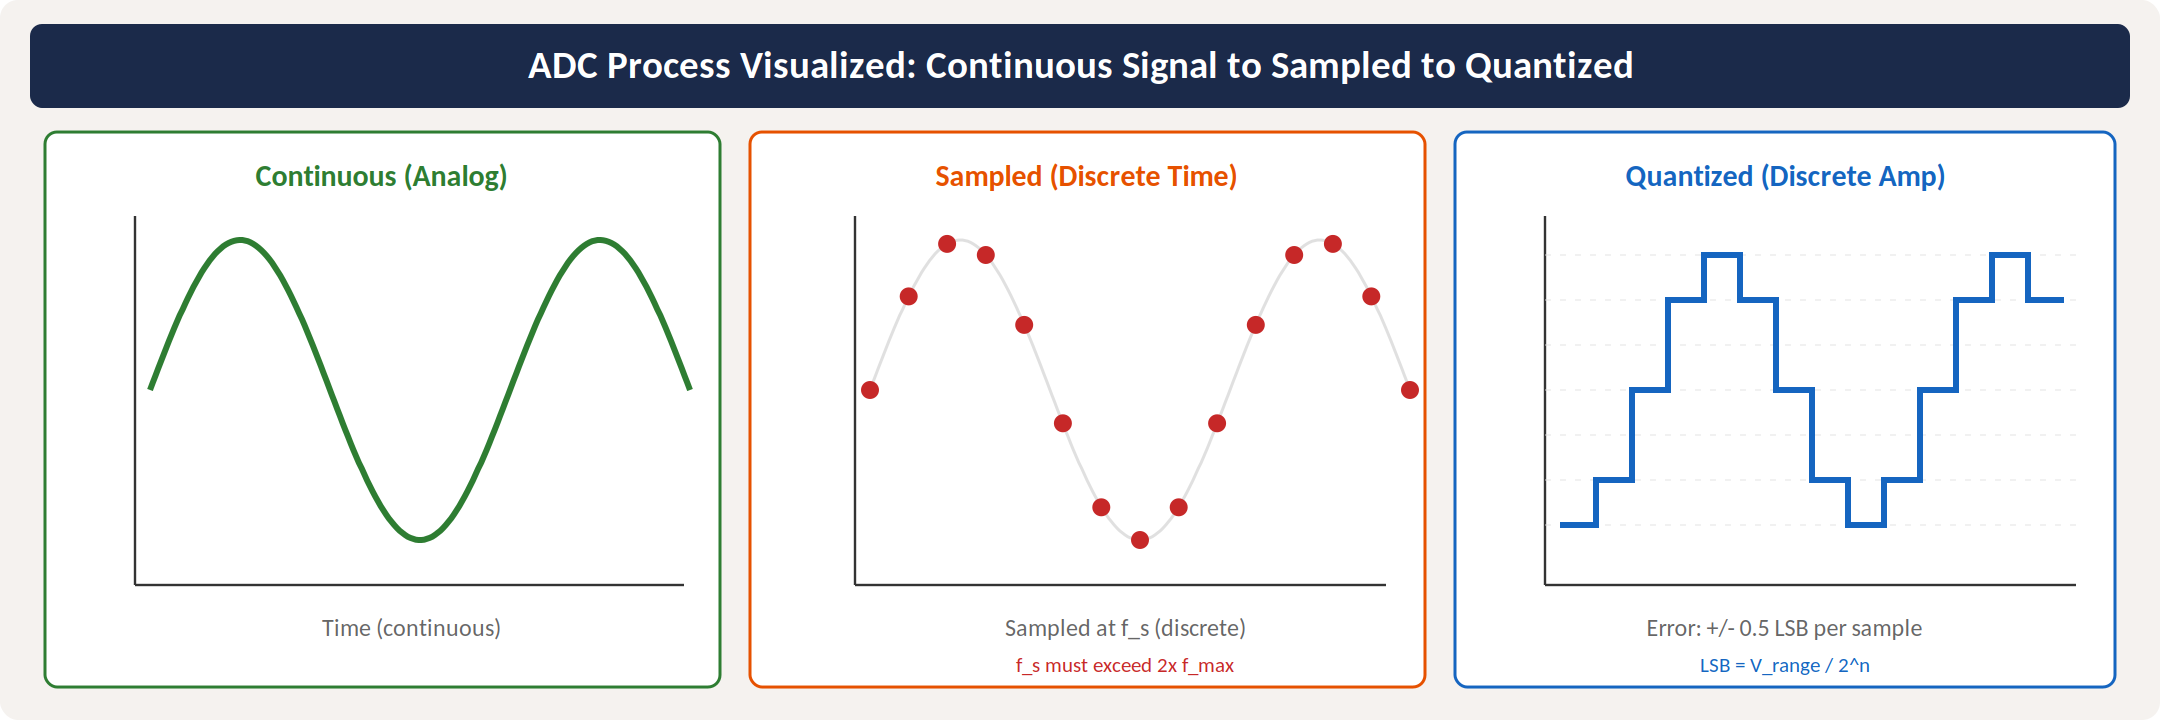
\includegraphics[width=\textwidth]{fig_adc_process.png}
\caption{The three critical aspects of analog-to-digital conversion: sampling rate, quantization resolution, and key specifications.}
\label{fig:adc}
\end{figure}

\section{Digital-to-Analog Conversion (DAC)}
A DAC converts a digital number back to an analog voltage. Used in control systems (Chapter~16) to drive actuators, in signal generators, and in audio output. Key parameters: resolution (bits), settling time, and output voltage range.

\section{Advantages and Trade-offs}
\begin{table}[htbp]\centering\small
\begin{tabularx}{\textwidth}{l X X}
\toprule
\textbf{Property} & \textbf{Analog} & \textbf{Digital} \\
\midrule
Noise immunity & Low; noise accumulates through the chain & High; regenerated at each stage \\
Precision & Limited by component tolerances & Limited by bit depth; easily $>$16 bits \\
Storage & Degrades over time (tape, film) & Perfect copies indefinitely \\
Processing & Real-time, continuous & Requires sampling; introduces latency \\
Flexibility & Fixed function hardware & Software-reconfigurable \\
Cost for precision & Expensive (matched components) & Cheap (digital computation) \\
\bottomrule
\end{tabularx}
\end{table}

\begin{tipbox}[Keep the Analog Path Clean, Do the Math Digitally]
The best practice in modern instrumentation: use high-quality analog signal conditioning (amplification, anti-alias filtering) to bring the signal into the ADC's optimal input range, then do all processing (calibration, filtering, FFT, averaging) in software. This minimizes analog component count and maximizes flexibility.
\end{tipbox}


\section{Sample-and-Hold (S/H)}
An ADC takes a finite time to complete a conversion (the \textbf{aperture time}). If the input voltage changes during conversion, the result is erroneous. A sample-and-hold circuit captures the analog voltage on a capacitor at the sampling instant and holds it constant while the ADC converts. Most modern ADCs include an internal S/H, but at high sampling rates or with fast-changing signals, the S/H settling time becomes a limitation.

\textbf{Aperture jitter}: random variation in the sampling instant. Creates timing uncertainty that converts to amplitude noise. For a sinusoidal signal of frequency $f$ and amplitude $V_p$:
\begin{equation}
V_{\text{noise,jitter}} = 2\pi f \cdot V_p \cdot t_{\text{jitter}}
\end{equation}
At high frequencies, jitter becomes the dominant noise source, limiting effective resolution.

\section{Multiplexing}
A DAQ system often uses a single ADC shared among multiple input channels via an \textbf{analog multiplexer} (MUX). The MUX switches channels sequentially, so the effective per-channel sampling rate is $f_s / N_{\text{channels}}$. This introduces a \textbf{channel-to-channel skew}: adjacent channels are sampled at slightly different times.

\begin{warningbox}[Channel Skew in Multiplexed DAQs]
If you need simultaneous sampling of multiple channels (e.g., correlating vibration and pressure), a multiplexed DAQ introduces timing errors. The NI~USB-6001 (multiplexed) has channel skew; the NI~USB-6356 (simultaneous sampling) does not. For timing-critical multi-channel measurements, use a simultaneous-sampling DAQ or synchronize channels with an external trigger.
\end{warningbox}

\section{Common NI DAQ Devices for MEGN 300}
\begin{table}[htbp]\centering\small
\begin{tabularx}{\textwidth}{l c c c c X}
\toprule
\textbf{Device} & \textbf{AI Ch} & \textbf{Resolution} & \textbf{Max Rate} & \textbf{Range} & \textbf{Notes} \\
\midrule
USB-6001 & 8 diff / 4 SE & 14-bit & 20\,kS/s & $\pm$10\,V & Basic; multiplexed \\
USB-6002 & 8 diff / 4 SE & 16-bit & 50\,kS/s & $\pm$10\,V & Higher resolution \\
USB-6009 & 8 diff / 4 SE & 14-bit & 48\,kS/s & $\pm$10\,V & Common in teaching labs \\
USB-6356 & 8 AI & 16-bit & 1.25\,MS/s & $\pm$10\,V & Simultaneous sampling \\
\bottomrule
\end{tabularx}
\caption{Common NI DAQ devices for MEGN~300 labs.}
\end{table}


\section{The Analog World and Its Limitations}
The physical world is inherently analog: temperature, pressure, velocity, and strain are continuous quantities that vary smoothly in both time and amplitude. Analog signals are vulnerable to noise, drift, and degradation during transmission. Every amplifier adds noise, every cable picks up electromagnetic interference, and analog storage degrades with time. This is why modern instrumentation converts signals to digital form as early as possible.

\section{Sampling Theory}
Sampling converts a continuous-time signal into a discrete-time sequence. The Nyquist-Shannon sampling theorem states: a bandlimited signal with maximum frequency $f_{\max}$ can be perfectly reconstructed from its samples if $f_s > 2f_{\max}$. The frequency $f_s/2$ is the Nyquist frequency. Any content above it aliases into the baseband and cannot be removed digitally. The only defense is an analog anti-alias filter before the ADC.

In practice, use $f_s \geq 10 \times f_{\max}$ for general measurement, $f_s \geq 20 \times f_{\text{bandwidth}}$ for control systems, and $f_s = 2.56 \times f_{\max}$ for vibration analysis.

\begin{warningbox}[Anti-Alias Filter Is Mandatory]
An analog low-pass filter must be present before the ADC in every properly designed system. It cannot be implemented in software because aliasing occurs at the moment of sampling. Set the cutoff at or below $f_s/2$ with sufficient rolloff (4th order minimum) to attenuate out-of-band content by at least 60\,dB.
\end{warningbox}

\section{Quantization in Depth}
An $n$-bit ADC divides $V_{\text{range}}$ into $2^n$ levels. The LSB voltage is $V_{\text{range}}/2^n$. Quantization error is $\pm$0.5\,LSB with RMS value $\text{LSB}/\sqrt{12}$. For $\pm$10\,V range: 12-bit gives 4.88\,mV LSB; 14-bit gives 1.22\,mV; 16-bit gives 0.305\,mV. Each additional bit halves the LSB.

The Effective Number of Bits (ENOB) quantifies actual resolution: ENOB $= (\text{SINAD} - 1.76)/6.02$. A 16-bit ADC may have ENOB of only 13--14 at full speed. Always check ENOB in the datasheet.

\section{Sample-and-Hold and Aperture Effects}
The ADC needs a stable input during conversion. A sample-and-hold (S/H) captures the signal at a precise instant. Without it, fast-changing signals cause aperture error: $\epsilon = 2\pi f \cdot A \cdot t_a$ where $t_a$ is the aperture time. For $<$0.5\,LSB error: $t_a < \text{LSB}/(2\pi f A)$.

\section{Multiplexing and Channel Skew}
Most DAQ devices share one ADC among channels via a multiplexer, introducing interchannel delay. For slowly varying signals this is negligible. For fast signals or phase-sensitive measurements, channel skew distorts results. Solutions: reduce active channels, use simultaneous sample-and-hold, or correct mathematically.

\section{Input Configuration}
\textbf{Differential}: measures $V_+ - V_-$. Rejects common-mode voltages. Mandatory for millivolt signals (thermocouples, bridges). Uses two channels per measurement.

\textbf{RSE (Referenced Single-Ended)}: measures voltage relative to DAQ ground. Suitable for volt-level grounded sources. Susceptible to ground loops.

\textbf{NRSE}: measures relative to a shared analog return. Useful for floating sources.

Always select the smallest input range that encompasses the signal. Using $\pm$10\,V for a 0--2\,V signal wastes 80\% of dynamic range, losing 2.3 bits of effective resolution.

\begin{examplebox}[ThermoRig: DAQ Configuration]
NI USB-6001: thermocouple signal (amplified to 0--4\,V by INA) on AI0+/AI0$-$ in Differential mode. Range: 0--5\,V. Rate: 100\,S/s ($10\times$ the 10\,Hz signal bandwidth). 14-bit resolution gives LSB $= 0.305$\,mV $\approx 0.007$\,\degC{} (well below sensor uncertainty). Anti-alias: 2nd-order Sallen-Key LP at 40\,Hz before the DAQ.
\end{examplebox}

\section{Digital-to-Analog Conversion}
DACs convert digital codes to analog voltages for control signals, excitation waveforms, and test stimuli. Key specs: resolution (bits), settling time, glitch energy, and monotonicity. A reconstruction low-pass filter smooths the DAC's staircase output.


\section{Understanding ADC Architectures}
Different applications require different ADC types. \textbf{Successive Approximation (SAR)}: the most common for data acquisition. Moderate speed (1\,kS/s to 5\,MS/s), moderate resolution (12--18 bits). One sample per conversion clock. Ideal for multiplexed multichannel systems.

\textbf{Sigma-Delta ($\Sigma\Delta$)}: extreme oversampling with noise shaping. Very high resolution (24 bits) at low to moderate bandwidth (10\,S/s to 100\,kS/s). Best for precision DC and low-frequency measurement (bridges, thermocouples). The NI USB-9219 uses sigma-delta.

\textbf{Flash}: fastest (100\,MS/s to 1\,GS/s) but lowest resolution (6--8 bits). Used in oscilloscopes and radar.

\textbf{Pipeline}: high speed with moderate resolution (10--14 bits at 10--200\,MS/s). Used in communications and high-speed data acquisition.

\section{Practical DAQ Considerations}
\textbf{Trigger modes}: start acquisition on an external signal (rising edge, level), software command, or internal timer. Hardware triggering enables synchronized measurement with external events (impact, valve opening).

\textbf{Buffer management}: the DAQ fills a hardware buffer (typically 4096--65536 samples). If software does not read the buffer before it fills, samples are lost (buffer overflow). In LabVIEW, the DAQ Read VI must execute faster than the buffer fill rate.

\textbf{Timing modes}: finite acquisition (acquire exactly $N$ samples, then stop) vs.\ continuous acquisition (run indefinitely, processing data in blocks). Continuous mode is standard for real-time monitoring and control.

\textbf{Synchronization}: when using multiple DAQ devices or combining analog and digital I/O, ensure all channels share a common clock and trigger to avoid timing skew.
\section{ADC Architecture Comparison}
Different applications demand different ADC types, and understanding the tradeoffs is essential for selecting the right DAQ hardware.

\textbf{Successive Approximation Register (SAR)}: uses a binary search algorithm, testing one bit per clock cycle. $n$ bits require $n$ clock cycles. Speed: 1\,kS/s to 5\,MS/s. Resolution: 12--18 bits. Low power. The most common architecture for general-purpose data acquisition. The NI USB-6001 uses a 14-bit SAR ADC.

\textbf{Sigma-Delta ($\Sigma\Delta$)}: oversamples at $64\times$--$256\times$ the output rate, shapes quantization noise to high frequencies, then decimation-filters to the output bandwidth. Very high resolution (24 bits) at low to moderate output rates (10--100\,kS/s). Best for precision DC and low-frequency measurement. The NI USB-9219 uses 24-bit sigma-delta.

\textbf{Flash}: uses $2^n - 1$ comparators operating simultaneously. Fastest (100\,MS/s to multi-GS/s) but limited resolution (6--8 bits) and high power. Used in oscilloscopes.

\textbf{Pipeline}: cascades multiple low-resolution stages, each refining the previous stage's residual error. High speed (10--200\,MS/s) with moderate resolution (10--14 bits). Used in communications and high-speed data acquisition.

\section{Practical DAQ Configuration Details}
\subsection{Trigger Configuration}
\textbf{Software trigger}: acquisition starts when the program calls the start function. Simple but introduces variable latency (milliseconds to tens of milliseconds) due to OS scheduling.

\textbf{Hardware trigger}: acquisition starts on an external electrical signal (rising/falling edge on a digital input, or analog level crossing). Precise timing ($<$1\,$\mu$s jitter). Essential for synchronizing acquisition with external events.

\textbf{Pre-trigger}: the DAQ continuously acquires data into a circular buffer and, upon trigger, saves the $N$ most recent samples plus $M$ post-trigger samples. This captures events that happen before the trigger point, which is essential for analyzing what caused the trigger event.

\subsection{Buffer Management and Data Throughput}
The DAQ writes samples to a hardware FIFO buffer. The software must read this buffer before it overflows. At 100\,kS/s with a 4096-sample buffer: the buffer fills in 41\,ms. The LabVIEW loop must execute a DAQ Read every 41\,ms at minimum. In practice, read every 10\,ms (1000 samples per read) to provide safety margin. If the loop is slower (due to disk I/O, display updates, or heavy computation), increase the buffer size or reduce the sample rate.

\subsection{Clock Sources}
The DAQ's internal clock provides adequate accuracy ($\pm$50\,ppm typical, or $\pm$5\,Hz at 100\,kS/s) for most applications. For measurements requiring precise frequency accuracy (vibration analysis, phase measurement), use an external clock from a precision oscillator or GPS-disciplined source. For multi-device synchronization, route the master clock from one DAQ to the clock input of the others.

\section{Grounding and Wiring Best Practices for DAQ}
\textbf{Twisted pair}: twist the signal and return wires together (2--4 turns per inch). This cancels magnetically induced noise because each half-twist receives equal but opposite induced voltage. Use twisted pair for all analog signals longer than 30\,cm.

\textbf{Shielded cable}: use shielded twisted pair for millivolt-level signals (thermocouples, bridges) or in high-EMI environments (near motors, power electronics). Connect the shield at the DAQ end only; leave it unconnected at the sensor end to avoid ground loops.

\textbf{Star grounding}: all analog grounds converge at a single point near the DAQ's analog ground terminal. Never daisy-chain grounds from one sensor to the next; the current from sensor~1 flowing through the shared ground wire creates a voltage drop that offsets sensor~2.

\textbf{Cable routing}: keep analog signal cables at least 30\,cm from power cables, motor cables, and switching circuits. Cross at right angles when cables must intersect. Never bundle analog and power cables in the same conduit.

\begin{warningbox}[The Most Expensive Mistake in Student Projects]
Using a breadboard for signal conditioning circuits in a final project is the most common cause of mysterious noise, intermittent failures, and unreproducible results. Breadboard contacts have variable resistance (0.01--1\,$\Omega$), parasitic capacitance (2--5\,pF per row), and poor high-frequency behavior. For millivolt-level signals, solder all connections to a protoboard or use a custom PCB. Reserve the breadboard for initial prototyping only.
\end{warningbox}
\section{Data Conversion Pipeline}
The complete data pipeline from analog sensor to engineering units involves multiple conversion stages, each with its own error contribution:

(1)~\textbf{Sensor}: physical quantity $\to$ electrical signal. Error: sensor accuracy, linearity, hysteresis.

(2)~\textbf{Signal conditioning}: raw electrical $\to$ conditioned electrical (amplified, filtered). Error: gain error, offset, noise.

(3)~\textbf{ADC}: conditioned voltage $\to$ digital code. Error: quantization ($\pm$0.5\,LSB), DNL/INL, aperture jitter.

(4)~\textbf{Calibration equation}: digital code $\to$ engineering units. Error: calibration residual, interpolation.

(5)~\textbf{Digital processing}: raw engineering units $\to$ processed result (filtered, averaged, derived quantities). Error: rounding, truncation, filter transients.

Each stage's error can be analyzed independently and combined via RSS to produce the total system uncertainty.

\section{Common ADC Errors}
\textbf{Differential nonlinearity (DNL)}: the deviation of any ADC step from the ideal 1\,LSB width. DNL $> +1$\,LSB means a missing code (some digital values are never output). For the NI USB-6001: DNL $< \pm$1\,LSB (no missing codes guaranteed).

\textbf{Integral nonlinearity (INL)}: the maximum deviation of the ADC's transfer function from the ideal straight line. INL affects the overall measurement accuracy (not just the step-to-step accuracy). For the NI USB-6001: INL $< \pm$4\,LSB at 14-bit.

\textbf{Aperture jitter}: variation in the exact sampling instant from sample to sample. For a sinusoidal signal at frequency $f$, aperture jitter $\sigma_t$ produces noise: $\text{SNR}_{\text{jitter}} = -20\log_{10}(2\pi f \sigma_t)$\,dB. At $f = 10$\,kHz and $\sigma_t = 50$\,ps: $\text{SNR} = 90$\,dB (adequate for 14-bit). At $f = 1$\,MHz: $\text{SNR} = 50$\,dB (limits effective resolution to $\sim$8 bits).

\section{Oversampling for Improved Resolution}
When oversampling by a factor $K$ and then digitally low-pass filtering and decimating, the effective resolution improves by approximately $\log_2(\sqrt{K})$ bits. To gain 1 bit of effective resolution: oversample by $4\times$. To gain 2 bits: $16\times$. To gain 4 bits (equivalent to upgrading from 12-bit to 16-bit): $256\times$.

Example: the NI USB-6001 (14-bit) sampling at 40\,kS/s with a 100\,Hz signal bandwidth provides $K = 40000/(2 \times 100) = 200\times$ oversampling. Theoretical resolution improvement: $\log_2(\sqrt{200}) = 3.8$ bits, giving effective 17.8-bit resolution. In practice, noise and INL limit the actual improvement to approximately 2--3 bits (16--17 bit effective). Still, this is a significant improvement from a simple, inexpensive DAQ device.
\section{Signal Conditioning Integration with DAQ}
The signal conditioning stage must be designed as a unit with the DAQ, not independently. Key integration points:

\textbf{Voltage range matching}: the maximum output of the signal conditioning must equal the ADC's full-scale input. Wasting 50\% of the input range (e.g., a 0--2.5\,V signal on a 0--5\,V range) costs one bit of effective resolution. Wasting 90\% (0--0.5\,V on 0--5\,V) costs over 3 bits.

\textbf{Impedance matching}: the signal conditioning output impedance must be low enough to charge the ADC's input sampling capacitor within the acquisition time. For a SAR ADC acquiring at 100\,kS/s with $C_{\text{sample}} = 20$\,pF: the source impedance should be $< 1/(2\pi \times 100000 \times 20 \times 10^{-12}) \approx 80$\,k$\Omega$. Most op-amp outputs have $< 100\,\Omega$ impedance, so this is rarely an issue unless you omit the output buffer.

\textbf{Common-mode voltage}: the ADC input has a limited common-mode range (typically $-0.2$\,V to $V_{\text{supply}} + 0.2$\,V for single-supply devices). If the signal conditioning output includes a common-mode voltage outside this range (e.g., a thermocouple referenced to earth ground while the DAQ is on USB ground), the ADC produces erroneous readings or damage. Use differential inputs or add a level-shifting circuit.

\section{Multi-Channel Acquisition Strategies}
\textbf{Sequential scanning}: the MUX connects each channel to the single ADC in turn. Channel rate $= f_s / N_{\text{channels}}$. For 8 channels at 100\,kS/s total: each channel sampled at 12.5\,kS/s. Interchannel delay $= 1/100000 = 10\,\mu$s.

\textbf{Simultaneous sample-and-hold (SSH)}: all channels have dedicated S/H circuits that capture simultaneously, then the single ADC converts each held value sequentially. No channel skew. Available on higher-end DAQ devices (NI USB-6356).

\textbf{Channel-to-channel crosstalk}: imperfect MUX isolation allows signal from one channel to leak into the next. Typical crosstalk: $-80$\,dB. For a 5\,V signal on channel 0, the leakage onto channel 1 is $5 \times 10^{-4} = 0.5$\,mV. If channel 1 measures a millivolt-level signal, this crosstalk is significant. Solution: separate high-voltage and low-voltage channels, or insert ground channels between them.

\section{Timing Verification}
In real-time systems, verify that the LabVIEW loop executes within the required period. Add a ``Tick Count'' function at the start and end of the loop and compute the elapsed time. If the loop occasionally exceeds the period (a ``timing violation''), samples may be lost or the control output may be delayed. Common causes: disk I/O (file write), display updates (front panel), and garbage collection. Solutions: move file writes to a separate parallel loop; reduce front panel update rate to 10\,Hz; pre-allocate arrays.
\section{Real-World DAQ System Examples}
\subsection{NI USB-6001 (MEGN 300 Standard)}
14-bit SAR ADC, 8 AI channels (4 differential), $\pm$10\,V or $\pm$1\,V range, 20\,kS/s aggregate (shared among active channels), 2 AO channels (12-bit), 13 DIO lines. USB-powered. Cost: $\sim$\$200. Adequate for temperature, strain, and low-frequency vibration measurements. Limited by: single ADC with multiplexer (channel skew), moderate resolution (14-bit), and USB latency ($\sim$1\,ms).

\subsection{NI USB-9234 (Vibration/Acoustics)}
24-bit delta-sigma ADC, 4 AI channels with simultaneous sampling, $\pm$5\,V range, 51.2\,kS/s per channel, built-in IEPE excitation for accelerometers, built-in anti-alias filters (software-configurable cutoff). Cost: $\sim$\$1{,}200. The standard for vibration analysis: high resolution, no channel skew, and integrated signal conditioning.

\subsection{Arduino/ESP32 (Embedded/Low-Cost)}
12-bit SAR ADC (10-bit on older Arduino), 0--3.3\,V input range, $\sim$1--100\,kS/s depending on configuration. No built-in anti-alias filter, no differential input, moderate noise (2--5\,LSB). Cost: \$5--\$15. Suitable for slow, non-critical measurements (ambient temperature monitoring, battery voltage). Inadequate for precision measurement without external signal conditioning.

\section{Practical Input Range Optimization}
The effective resolution of an ADC depends on how well you use its input range. Define the \textbf{range utilization ratio} $U = V_{\text{signal, pk-pk}} / V_{\text{ADC, range}}$.

If $U = 1.0$ (signal fills the entire range): you use all $n$ bits. If $U = 0.5$ (signal uses half the range): you lose 1 bit (equivalent to $n-1$ bit ADC). If $U = 0.1$ (signal uses 10\%): you lose 3.3 bits.

\textbf{Design strategy}: set the signal conditioning gain so that the maximum expected signal (plus noise margin) reaches 80--90\% of the ADC's full-scale input. Leave 10--20\% headroom for unexpected peaks, noise spikes, and component tolerances. This maximizes the effective resolution while preventing clipping.

Example: thermocouple conditioned by INA128 with $G = 611$. Maximum TC output at 200\,\degC{}: $200 \times 0.041 = 8.2$\,mV. After amplification: $8.2 \times 611 = 5.01$\,V. Using the 0--5\,V DAQ range: $U = 5.01/5.0 = 1.0$. Excellent range utilization. But with the default $\pm$10\,V range: $U = 5.01/20 = 0.25$, losing 2 bits of effective resolution.

\section{Timing Accuracy and Jitter}
The accuracy of time-domain measurements (period, frequency, phase) depends on the sampling clock accuracy and jitter:

\textbf{Clock accuracy}: the NI~USB-6001 internal clock has $\pm$50\,ppm accuracy. At 10\,kS/s: the actual rate is $10{,}000 \pm 0.5$\,S/s. Over a 10-second acquisition: the timing error accumulates to $\pm$5\,$\mu$s. This is negligible for most measurements but significant for precise frequency measurement (use an external crystal oscillator or GPS-disciplined clock for $< 1$\,ppm accuracy).

\textbf{Clock jitter}: sample-to-sample variation in the sampling instant. Typical: 50--500\,ps for a DAQ internal clock. Jitter produces noise proportional to signal frequency: SNR$_{\text{jitter}} = -20\log_{10}(2\pi f \sigma_j)$. At $f = 1$\,kHz, $\sigma_j = 200$\,ps: SNR $= 118$\,dB (far below the ADC noise floor; negligible). At $f = 10$\,MHz, $\sigma_j = 200$\,ps: SNR $= 58$\,dB (limits effective resolution to $\sim$9 bits). Jitter is only a concern for high-frequency signals.
\section{Practice Questions}
\begin{enumerate}[leftmargin=1.5em]
\item A 16-bit ADC has an input range of 0--10\,V. Calculate the LSB voltage and the maximum quantization error in millivolts.
\item Your sensor outputs 0--50\,mV for the full measurement range. Your ADC has a 0--5\,V input range and 12-bit resolution. What amplifier gain do you need, and what is the resulting measurement resolution in terms of the sensor output?
\item Explain why a digital system has better noise immunity than an analog system for transmitting data over a long cable.
\end{enumerate}

\subsection{Answers}
\begin{enumerate}[leftmargin=1.5em]
\item LSB $= 10 / 2^{16} = 10/65536 = 0.153$\,mV. Max quantization error $= \pm 0.5 \times 0.153 = \pm 0.076$\,mV.
\item Gain $= 5\,\text{V} / 0.050\,\text{V} = 100$. Amplified LSB $= 5/(4096) = 1.22$\,mV at the ADC. Referred to the sensor input: $1.22/100 = 0.0122$\,mV $= 12.2$\,$\mu$V. Sensor resolution $= 12.2\,\mu$V $/ (50\,\text{mV}/\text{FS}) = 0.024\%$ FS.
\item A digital signal has only two states (0 and 1). As long as noise does not push the signal past the decision threshold, the receiver reconstructs the original data perfectly. An analog signal carries information in continuous voltage levels; any noise added to the signal is indistinguishable from the signal itself and permanently corrupts the measurement.
\end{enumerate}


% ================================================================
\chapter{Signal-to-Noise Ratio}

\section{Defining SNR}
The signal-to-noise ratio quantifies how much useful signal exists relative to unwanted noise:
\begin{equation}
\text{SNR} = \frac{P_{\text{signal}}}{P_{\text{noise}}} = \left(\frac{V_{\text{signal,RMS}}}{V_{\text{noise,RMS}}}\right)^2
\end{equation}
In decibels:
\begin{equation}
\text{SNR}_{\text{dB}} = 10 \log_{10}\left(\frac{P_{\text{signal}}}{P_{\text{noise}}}\right) = 20 \log_{10}\left(\frac{V_{\text{signal,RMS}}}{V_{\text{noise,RMS}}}\right)
\end{equation}
A 20\,dB SNR means the signal is 10$\times$ the noise voltage. A 40\,dB SNR means 100$\times$. An ADC with $n$ bits has a theoretical maximum SNR of $6.02n + 1.76$\,dB (e.g., 12-bit $\to$ 74\,dB).

\section{Noise Sources in Instrumentation}
\textbf{Thermal noise} (Johnson-Nyquist): $V_n = \sqrt{4k_B T R \Delta f}$, present in every resistor. Reduced by cooling, lowering resistance, or narrowing bandwidth.

\textbf{Shot noise}: caused by discrete charge carriers crossing a junction. Proportional to $\sqrt{I \cdot \Delta f}$.

\textbf{Flicker noise} ($1/f$ noise): dominant at low frequencies. Reduced by chopper-stabilized amplifiers or AC-coupling.

\textbf{Electromagnetic interference} (EMI): coupled from external sources (power lines at 60\,Hz, switching regulators, motors). Reduced by shielding, twisted pairs, differential signaling, and filtering.

\textbf{Quantization noise}: inherent in ADCs (Chapter~5). Reduced by using higher resolution.

\begin{figure}[htbp]
\centering
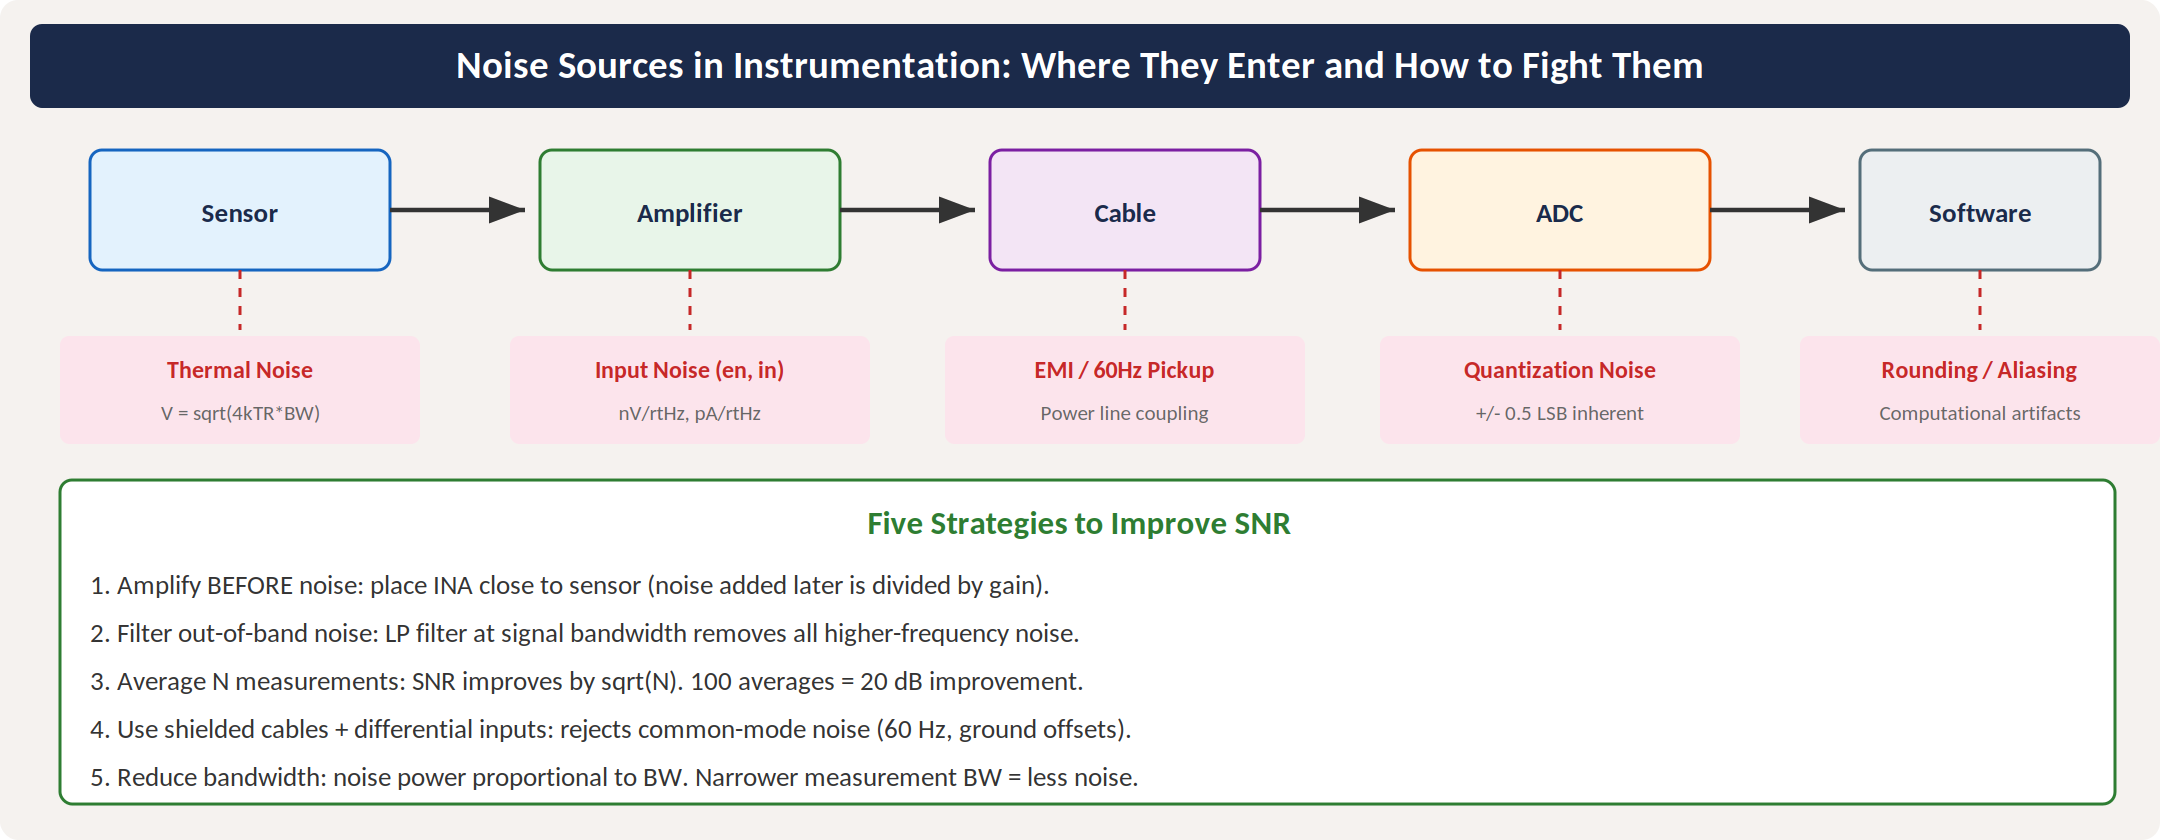
\includegraphics[width=\textwidth]{fig_noise_sources.png}
\caption{Five noise sources in the measurement chain and five strategies to combat them. The key insight: amplify before noise enters the chain; noise added after amplification is divided by the gain.}
\label{fig:noise_sources}
\end{figure}

\section{Improving SNR}
\begin{enumerate}[leftmargin=1.5em]
\item \textbf{Amplify the signal before the noise is added}. Place the amplifier as close to the sensor as possible.
\item \textbf{Filter out-of-band noise}. If your signal is 0--100\,Hz, a low-pass filter at 100\,Hz removes all higher-frequency noise.
\item \textbf{Average repeated measurements}. $n$ averages improve SNR by $\sqrt{n}$ ($10\log_{10}(n)$\,dB).
\item \textbf{Use shielded cables and differential signaling}. Rejects common-mode noise.
\item \textbf{Reduce bandwidth}. Noise power is proportional to bandwidth. Narrower measurement bandwidth $=$ less noise.
\end{enumerate}

\begin{warningbox}[60\,Hz Hum]
The most common noise source in lab measurements is 60\,Hz pickup from AC power lines. Symptoms: a clean-looking signal with a 60\,Hz ripple superimposed. Fixes: use shielded cables, ground the shield at one end only, keep signal wires away from power cables, use differential inputs on the DAQ, and add a 60\,Hz notch filter in software.
\end{warningbox}


\section{Dynamic Range}
The \textbf{dynamic range} of a measurement system is the ratio of the largest measurable signal to the smallest detectable signal (noise floor):
\begin{equation}
\text{DR}_{\text{dB}} = 20 \log_{10}\left(\frac{V_{\text{max}}}{V_{\text{noise floor}}}\right)
\end{equation}
For an ideal $n$-bit ADC: $\text{DR} = 6.02n + 1.76$\,dB. A 16-bit ADC has a theoretical dynamic range of 98\,dB, meaning it can resolve signals spanning a 79,000:1 voltage ratio.

\section{Grounding Best Practices for Low-Noise Measurements}
\begin{enumerate}[leftmargin=1.5em]
\item \textbf{Single-point (star) ground}: all ground returns meet at one physical point near the power supply. Prevents ground loops.
\item \textbf{Differential inputs}: measure the voltage difference between two wires, rejecting common-mode noise (60\,Hz hum, ground offsets). Always use differential mode on NI DAQs when measuring bridge circuits, thermocouples, or any sensor in a noisy environment.
\item \textbf{Shielded cables}: the shield connects to ground at \emph{one end only} (typically the DAQ end). Grounding at both ends creates a ground loop that couples noise.
\item \textbf{Twisted pairs}: twisting the signal and return wires reduces magnetic pickup because induced voltages cancel in adjacent twists.
\item \textbf{Physical separation}: route signal cables at least 30\,cm from power cables. Cross at right angles if they must cross.
\end{enumerate}

\begin{examplebox}[ThermoRig: Diagnosing 60\,Hz Noise]
The ThermoRig thermocouple signal shows a clean 25\,\degC{} reading on the benchtop but develops $\pm$0.3\,\degC{} oscillation when the heater is powered on. FFT reveals a dominant 60\,Hz peak. Root cause: the heater power cable runs parallel to the thermocouple extension wire for 50\,cm. Fix: (1) reroute the thermocouple wire away from the heater cable, (2) switch the DAQ to differential input mode, (3) add a 50-point moving average in LabVIEW (effective cutoff well below 60\,Hz given the slow thermal process). Result: noise drops to $\pm$0.02\,\degC{}.
\end{examplebox}


\section{Defining Signal and Noise}
The signal carries information about the measurand; noise is everything else. Noise is present at every stage and can never be eliminated completely. The goal is to make the signal large relative to the noise.

\section{The Decibel Scale}
SNR in decibels: $\text{SNR} = 20\log_{10}(V_s/V_n)$\,dB. Reference: 0\,dB means signal equals noise. 20\,dB means $10\times$. 40\,dB means $100\times$. 60\,dB means $1000\times$. Maximum theoretical ADC SNR: $6.02n + 1.76$\,dB. Doubling signal power adds 3\,dB; doubling voltage adds 6\,dB; $10\times$ voltage adds 20\,dB.

\section{Noise Classification}
\textbf{Thermal noise}: $V_n = \sqrt{4k_BTR B}$. At 300\,K, a 10\,k$\Omega$ resistor over 10\,kHz: $V_n = 1.28$\,$\mu$V. This is the fundamental noise floor.

\textbf{Shot noise}: $I_n = \sqrt{2qI_{DC}B}$. Appears in semiconductor junctions.

\textbf{Flicker (1/f) noise}: increases at low frequencies. Dominant below $\sim$1\,kHz in semiconductors. Makes precision DC measurements harder than AC.

\textbf{EMI}: 60\,Hz from power lines (capacitive and inductive coupling), switching supply harmonics (100\,kHz--1\,MHz), motor commutation, fluorescent lighting. EMI has specific frequencies visible as FFT spikes.

\section{Grounding Best Practices}
\textbf{Single-point (star) ground}: all grounds connect at one point. Prevents ground loops.

\textbf{Separate analog/digital grounds}: digital switching noise must not contaminate analog signal paths. Connect grounds only at the star point.

\textbf{Shield grounding}: connect cable shields at one end only (DAQ end). Both-end grounding creates a ground loop.

\textbf{Decoupling}: 100\,nF ceramic at every IC power pin, 10\,$\mu$F electrolytic at each rail entry point.

\begin{examplebox}[ThermoRig: Diagnosing 60 Hz Noise]
Initial testing showed $\pm$2\,\degC{} oscillation at 60\,Hz (visible in FFT with harmonics at 120, 180, 240\,Hz). Root cause: heater cable ran parallel to thermocouple cable, coupling 60\,Hz capacitively. Fix: separated cables by 15\,cm, used shielded TC wire (shield grounded at DAQ), switched to Differential mode. Result: 60\,Hz spike dropped from 2\,\degC{} to 0.01\,\degC{}. Cost: \$0 and 10 minutes.
\end{examplebox}

\section{Noise in the Signal Chain}
Noise at the sensor end is amplified by the full system gain and dominates the output. Noise at the DAQ end is not amplified. \textbf{Golden rule}: amplify as early as possible, as close to the sensor as possible.

For a two-stage system with gains $G_1$ and $G_2$ and stage noise $V_{n,1}$, $V_{n,2}$: $V_{n,\text{out}} = \sqrt{(G_1 G_2 V_{n,\text{src}})^2 + (G_2 V_{n,1})^2 + V_{n,2}^2}$. The first stage's noise is amplified by $G_2$; the second stage's noise appears directly.

\section{SNR Improvement Techniques}
\textbf{Averaging}: $N$ averages reduces random noise by $\sqrt{N}$, improving SNR by $10\log_{10}(N)$\,dB. 100 averages $= +$20\,dB. Does not help with systematic errors or correlated noise.

\textbf{Filtering}: noise power $\propto$ bandwidth. Halving BW improves SNR by 3\,dB. Use the narrowest BW consistent with the signal.

\textbf{Differential inputs}: rejects common-mode interference (60\,Hz, ground offsets).

\textbf{Shielding}: Faraday cage around sensitive circuits blocks electric field coupling.

\textbf{Synchronous detection (lock-in)}: modulate signal at known frequency, extract with narrow-band detection. Can measure signals 60\,dB below the noise floor.


\section{Noise Spectral Density}
Noise is characterized by its power spectral density (PSD), measured in V$^2$/Hz (or equivalently nV/$\sqrt{\text{Hz}}$ for voltage noise density). The total noise voltage in a measurement with bandwidth $B$ is $V_n = e_n \sqrt{B}$ where $e_n$ is the noise density. This is why reducing measurement bandwidth directly reduces noise.

Op-amp noise density is specified on the datasheet as $e_n$ (input-referred voltage noise) and $i_n$ (input-referred current noise). For an op-amp with $e_n = 10$\,nV/$\sqrt{\text{Hz}}$ and bandwidth $B = 10$\,kHz: $V_n = 10 \times \sqrt{10000} = 1$\,$\mu$V RMS input-referred noise.

\section{Dynamic Range}
The dynamic range is the ratio between the largest and smallest signals the system can measure simultaneously: $\text{DR} = 20\log_{10}(V_{\max}/V_{\min,\text{detectable}})$\,dB. For an ideal $n$-bit ADC, $\text{DR} = 6.02n + 1.76$\,dB. In practice, noise limits the minimum detectable signal, reducing the effective dynamic range.

\section{Ground Loops: Diagnosis and Cure}
A ground loop occurs when two or more ground connections create a closed current path. Current flowing through the finite impedance of the ground conductor creates a voltage drop that appears as noise. Symptoms: large 60\,Hz component in the FFT, noise that changes when you touch the cable, noise that depends on the position of nearby equipment.

Diagnosis: disconnect the sensor. If the noise disappears, the ground loop is between the sensor and DAQ. If it persists, the loop is internal to the DAQ/computer.

Cure: (1) use differential inputs (measures between two signal wires, ignoring ground). (2) Use a single-point ground topology. (3) Insert an isolation amplifier or optocoupler to break the galvanic path. (4) Use battery-powered (floating) sensor excitation.

\section{EMI Shielding Effectiveness}
Cable shielding is characterized by its transfer impedance $Z_t$ (in $\Omega$/m), which describes how much external interference voltage appears on the inner conductor per unit length. Lower is better. Single-braid shield: $Z_t \approx 10$\,m$\Omega$/m at low frequencies. Double-braid: $\approx 1$\,m$\Omega$/m. Foil shield: excellent at high frequencies but poor at low frequencies due to limited coverage. For best performance, use a foil + braid combination.
\section{Noise Budget Analysis}
Just as an error budget allocates measurement uncertainty across the signal chain, a \textbf{noise budget} allocates the noise contribution of each component. The total output-referred noise is:
\begin{equation}
V_{n,\text{total}} = \sqrt{(G_{\text{total}} \cdot e_{n,\text{sensor}})^2 + (G_2 G_3 \cdot e_{n,\text{amp1}})^2 + (G_3 \cdot e_{n,\text{amp2}})^2 + e_{n,\text{ADC}}^2}
\end{equation}
where $G_i$ are the gains of each stage and $e_{n,i}$ are the input-referred noise voltages. The key insight: the first stage's noise is amplified by the full remaining gain, while later stages contribute progressively less.

\subsection{Worked Example}
Consider: sensor noise $e_n = 2\,\mu$V/$\sqrt{\text{Hz}}$, first amplifier (INA128) $e_n = 8$\,nV/$\sqrt{\text{Hz}}$ at gain $G_1 = 100$, second stage filter buffer $e_n = 15$\,nV/$\sqrt{\text{Hz}}$ at gain $G_2 = 1$, ADC noise floor 200\,$\mu$V RMS. System bandwidth 100\,Hz.

Sensor contribution at output: $100 \times 1 \times 2\,\mu\text{V} \times \sqrt{100} = 2{,}000\,\mu$V.
INA128 contribution: $1 \times 8\,\text{nV} \times \sqrt{100} = 0.08\,\mu$V (negligible).
Buffer contribution: $15\,\text{nV} \times \sqrt{100} = 0.15\,\mu$V (negligible).
ADC: 200\,$\mu$V (fixed).
Total: $\sqrt{2000^2 + 0.08^2 + 0.15^2 + 200^2} = 2010\,\mu$V.

The sensor dominates completely (99.5\% of noise power). A lower-noise amplifier would not improve the system. Reducing the sensor noise (e.g., by using a less noisy sensor type) or reducing the bandwidth (e.g., filtering at 10\,Hz instead of 100\,Hz, reducing sensor noise by $\sqrt{10} = 3.16\times$) are the only effective strategies.

\section{Common-Mode Rejection in Practice}
Common-mode voltage ($V_{CM}$) is the average voltage at the two differential inputs relative to ground. It represents ground offsets, 60\,Hz pickup, and other interference that appears equally on both input wires. The differential amplifier (or INA) rejects this common-mode signal while amplifying the differential signal.

CMRR is typically specified at DC (e.g., 120\,dB for INA128 at $G = 100$) but degrades at higher frequencies. At 60\,Hz, CMRR might be only 80--90\,dB. This is still excellent: 80\,dB CMRR means a 1\,V common-mode voltage at 60\,Hz produces only $1\,\text{V}/10{,}000 = 100\,\mu$V of interference at the output. For a thermocouple producing 4\,mV, this is a 2.5\% error, which is significant. Higher CMRR or better shielding/grounding is needed.

\section{Noise Figure}
The noise figure ($NF$) quantifies how much a component degrades the SNR:
\begin{equation}
NF = 10\log_{10}\left(\frac{\text{SNR}_{\text{in}}}{\text{SNR}_{\text{out}}}\right) \text{ dB}
\end{equation}
An ideal amplifier has $NF = 0$\,dB (adds no noise). Real amplifiers have $NF = 1$--$10$\,dB. The system noise figure is dominated by the first stage (Friis formula):
\begin{equation}
NF_{\text{total}} \approx NF_1 + \frac{NF_2 - 1}{G_1} + \frac{NF_3 - 1}{G_1 G_2} + \cdots
\end{equation}
With $G_1 = 100$: even if the second stage has $NF_2 = 10$\,dB ($F_2 = 10$), its contribution is $(10-1)/100 = 0.09$, adding only 0.04\,dB to the system noise figure. This mathematically confirms the golden rule: the first amplifier determines the system noise performance.

\section{Noise Measurement Techniques}
To characterize the noise of your measurement system: (1) Short the input (connect the two differential inputs together). (2) Acquire $N \geq 10{,}000$ samples at the normal operating sample rate. (3) Compute the RMS of the acquired data: this is the total system noise floor. (4) Compute the FFT: peaks at specific frequencies indicate EMI (60\,Hz, switching noise); a flat floor indicates thermal/shot noise.

Compare the measured noise to the theoretical prediction from the noise budget. If the measured noise significantly exceeds the prediction, look for: ground loops, EMI pickup, inadequate decoupling, or oscillating amplifiers.

\section{Signal Recovery from Noise}
\textbf{Coherent averaging (signal averaging)}: for repetitive signals (triggered waveforms), average $N$ acquisitions. Random noise cancels; the signal accumulates. SNR improves by $\sqrt{N}$. Used in oscilloscopes, vibration analyzers, and evoked-potential medical instruments.

\textbf{Correlation}: cross-correlate the measured signal with a reference waveform. The correlation peak indicates the presence and timing of the signal, even when buried in noise. This is the mathematical basis of lock-in amplification and GPS signal detection.

\textbf{Matched filtering}: design a filter whose impulse response matches the expected signal shape. The matched filter maximizes the SNR at the output for a known signal in white noise. Used in radar and communications.
\section{Noise Measurement Procedure for MEGN 300 Labs}
A systematic noise characterization should be performed as the first step in any lab:

(1)~\textbf{Short-input test}: connect AI+ to AI$-$ at the DAQ terminal block (zero signal). Acquire 10,000 samples at the operating sample rate. Compute the standard deviation: this is your system noise floor. Compare to the theoretical LSB noise: $\text{LSB}/\sqrt{12}$. If measured noise is $>3\times$ theoretical, there is excess noise from grounding, EMI, or power supply issues.

(2)~\textbf{Resistor-terminated test}: connect a precision resistor across the differential inputs equal to the sensor's output impedance. This includes the thermal noise of the resistor. Compare to the short-input noise: the increase is the thermal noise contribution.

(3)~\textbf{Sensor-connected test}: connect the actual sensor in the actual mounting configuration. Acquire with the same settings. This captures all real-world noise sources: sensor noise, cable pickup, ground loops, and environmental interference.

(4)~\textbf{FFT analysis}: compute the FFT of the noise data. Identify discrete peaks (60\,Hz, switching frequencies, resonances) vs.\ broadband floor. Address the discrete peaks first (grounding, shielding, filtering), then evaluate whether the broadband floor meets the SNR requirement.

\section{SNR Requirements for Different Measurement Types}
\textbf{Temperature monitoring ($\pm$1\,\degC{})}: SNR $> 40$\,dB is adequate. Easy to achieve with any modern DAQ.

\textbf{Strain measurement ($\pm$10\,$\mu\epsilon$)}: requires SNR $> 60$\,dB. Demands careful grounding, shielded cabling, and a low-noise INA.

\textbf{Vibration analysis (resolving 60\,dB dynamic range)}: requires SNR $> 80$\,dB. Requires IEPE accelerometers with built-in signal conditioning, differential transmission, and proper anti-alias filtering.

\textbf{Audio-quality measurement}: SNR $> 90$\,dB. Requires precision ADCs (24-bit sigma-delta), balanced signal paths, and low-noise power supplies.
\section{Quantifying EMI: Conducted vs. Radiated}
EMI enters the measurement circuit through two mechanisms:

\textbf{Conducted EMI}: noise current flowing on power supply lines, ground wires, or signal cables. The noise originates from switching power supplies, motor drives, or digital circuits, and propagates through shared conductors. Mitigation: ferrite beads on power lines, LC filters at power entry points, separate power supplies for analog and digital circuits.

\textbf{Radiated EMI}: electromagnetic fields from nearby sources (power lines, transformers, motors, RF transmitters, switching converters) couple into cables and circuits acting as antennas. Mitigation: shielding (Faraday cages, shielded cables), reducing cable loop area (twisted pair), increasing distance from the source (field strength decreases as $1/r^2$ for near-field sources).

The distinction matters for diagnosis: if noise disappears when you disconnect the signal cable (leaving the DAQ connected to nothing), the noise is conducted on the cable. If noise persists with the cable disconnected, it is radiated into the DAQ directly (or conducted on the power supply).

\section{Power Supply Noise}
The DAQ and signal conditioning circuits require clean power. A switching regulator (buck/boost) produces ripple at the switching frequency (typically 100\,kHz--2\,MHz) and its harmonics. This ripple appears on the power rail as a 10--50\,mV$_{\text{pk-pk}}$ sawtooth waveform that directly modulates the op-amp's output through the Power Supply Rejection Ratio (PSRR).

For an op-amp with PSRR $= 80$\,dB at 100\,kHz, a 20\,mV power supply ripple produces $20 \times 10^{-4} = 0.002$\,mV ($2\,\mu$V) at the output. At gain 1000, this becomes 2\,mV, which may be significant for millivolt-level measurements. Solution: use a linear regulator after the switching regulator (the linear regulator's PSRR further attenuates the switching noise by 40--60\,dB), or power the analog circuits from a separate linear supply.

\section{SNR Improvement: A Quantitative Case Study}
ThermoRig initial setup: thermocouple ($e_n = 2\,\mu$V$/\sqrt{\text{Hz}}$, measured at sensor), INA128 ($G = 611$), no anti-alias filter, RSE input mode, DAQ at $\pm$10\,V range, 1\,kS/s.

\textbf{Initial SNR}: signal at 80\,\degC{} $= 3.3$\,mV $\times 611 = 2.0$\,V. Noise at output: 120\,mV RMS (dominated by 60\,Hz at 80\,mV and broadband above 100\,Hz at 90\,mV). SNR $= 20\log(2.0/0.12) = 24$\,dB. Terrible.

\textbf{Fix 1}: switch to Differential mode. 60\,Hz drops from 80\,mV to 2\,mV ($\sim$30\,dB improvement in 60\,Hz component).

\textbf{Fix 2}: add 2nd-order anti-alias LP at 40\,Hz. Broadband noise above 40\,Hz removed. Remaining noise: 8\,mV RMS.

\textbf{Fix 3}: change input range from $\pm$10\,V to 0--5\,V ($4\times$ better resolution). Quantization noise drops below 0.3\,mV.

\textbf{Fix 4}: average 100 samples per reading (at 100\,S/s: 1\,s averaging time). Remaining random noise: $8/\sqrt{100} = 0.8$\,mV.

\textbf{Final SNR}: $20\log(2000/0.8) = 68$\,dB. Improved from 24\,dB to 68\,dB, a $44$\,dB ($160\times$) improvement, using only software and configuration changes (no hardware cost).
\section{Dynamic Range and Effective Bits}
The \textbf{dynamic range} of a measurement system is the ratio between the largest signal it can measure (without clipping) and the smallest signal it can detect (above the noise floor), expressed in dB:
\begin{equation}
\text{DR} = 20\log_{10}\left(\frac{V_{\text{max}}}{V_{\text{noise, RMS}}}\right) \text{ dB}
\end{equation}

For an ideal $n$-bit ADC: DR $= 6.02n + 1.76$\,dB. For the NI~USB-6001 (14-bit, $\pm$10\,V range): ideal DR $= 86$\,dB. In practice, noise from the signal conditioning chain reduces DR below the ideal. If the total system noise is 2\,mV RMS on a $\pm$10\,V range: DR $= 20\log_{10}(10/0.002) = 74$\,dB, equivalent to ENOB $= (74-1.76)/6.02 = 12.0$ effective bits. The signal conditioning has cost 2 bits of dynamic range.

This is why the noise budget matters: it directly determines how much of the ADC's resolution is actually usable.

\section{Noise Floor and Minimum Detectable Signal}
The minimum detectable signal (MDS) is typically defined as the signal level equal to the RMS noise floor (SNR $= 0$\,dB) or 3$\times$ the noise floor (SNR $= 10$\,dB, commonly used). Any signal below the MDS is buried in noise and cannot be reliably measured.

For the ThermoRig with 0.8\,mV total output noise (after all improvements): MDS $= 3 \times 0.8 = 2.4$\,mV, corresponding to $2.4/(611 \times 0.041) = 0.096$\,\degC{} at the thermocouple. Any temperature change smaller than 0.1\,\degC{} cannot be reliably detected. This is $10\times$ better than the $\pm$1\,\degC{} requirement, meaning the system has ample SNR margin.

\section{Noise in Data Acquisition Systems}
The total noise at the DAQ output includes contributions from multiple sources, combined by RSS:

\textbf{Sensor noise}: inherent to the sensor physics (thermal noise in resistive sensors, shot noise in photodiodes). Set by the sensor type and operating conditions.

\textbf{Signal conditioning noise}: op-amp voltage and current noise, resistor thermal noise in the gain and filter networks. Dominated by the first amplifier stage.

\textbf{EMI pickup}: 60\,Hz and harmonics from power lines, switching frequencies from nearby electronics. Reducible by shielding, grounding, and differential inputs.

\textbf{DAQ noise}: quantization noise ($\text{LSB}/\sqrt{12}$), ADC comparator noise, clock jitter. Fixed by the DAQ hardware; the only mitigation is choosing a better DAQ.

\textbf{Software noise}: rounding in calibration calculations, truncation in filter coefficients. Usually negligible with 64-bit double precision.

\section{Lock-In Amplification: Extracting Signals from Noise}
For the most demanding measurement applications (measuring signals 60--120\,dB below the noise floor), \textbf{lock-in amplification} uses synchronous detection. The principle:

(1) Modulate the measurand at a known reference frequency $f_{\text{ref}}$ (e.g., chop the light beam in an optical measurement). (2) Amplify the sensor signal, which now contains the desired signal at $f_{\text{ref}}$ plus broadband noise. (3) Multiply the amplified signal by a reference sine wave at $f_{\text{ref}}$ (the ``demodulation'' step). This shifts the signal to DC while spreading the noise across all frequencies. (4) Low-pass filter the result with a very narrow bandwidth (0.01--1\,Hz). The filter passes only the DC component (the desired signal) and rejects all noise except in the narrow band around $f_{\text{ref}}$.

The effective noise bandwidth is the LP filter bandwidth, not the signal bandwidth. A lock-in with 0.1\,Hz bandwidth on a system with 10\,kHz signal bandwidth achieves $10\log_{10}(10000/0.1) = 50$\,dB improvement in SNR. This is why lock-in amplifiers can detect nanovolt signals in millivolt noise.

While lock-in amplification is beyond the scope of MEGN~300 labs, understanding the principle illustrates the power of frequency-domain noise rejection and motivates the simpler techniques (averaging, filtering, differential inputs) used in your projects.
\section{Practice Questions}
\begin{enumerate}[leftmargin=1.5em]
\item A sensor produces 100\,mV\textsubscript{RMS} signal with 2\,mV\textsubscript{RMS} noise. Calculate the SNR in dB.
\item You average 64 measurements. By how many dB does the SNR improve?
\item A 14-bit ADC has a theoretical SNR of how many dB? If the noise floor is 0.5\,mV\textsubscript{RMS} and the input range is 0--5\,V, is the system noise-limited or quantization-limited?
\end{enumerate}

\subsection{Answers}
\begin{enumerate}[leftmargin=1.5em]
\item SNR $= 20\log_{10}(100/2) = 20\log_{10}(50) = 34.0$\,dB.
\item Improvement $= 10\log_{10}(64) = 18.1$\,dB.
\item Theoretical: $6.02 \times 14 + 1.76 = 86.0$\,dB. ADC LSB $= 5/2^{14} = 0.305$\,mV. Quantization noise RMS $= 0.305/\sqrt{12} = 0.088$\,mV. System noise floor is 0.5\,mV $\gg$ 0.088\,mV; the system is noise-limited, not quantization-limited. The extra ADC bits are wasted unless the noise is reduced.
\end{enumerate}


% ================================================================
\chapter{Fourier Series and Complex Signal Construction}

\section{The Fourier Principle}
Any periodic signal $x(t)$ with period $T$ can be represented as a sum of sinusoids at the fundamental frequency $f_0 = 1/T$ and its integer harmonics:
\begin{equation}
x(t) = \frac{a_0}{2} + \sum_{n=1}^{\infty} \left[ a_n \cos(2\pi n f_0 t) + b_n \sin(2\pi n f_0 t) \right]
\end{equation}
where the Fourier coefficients are:
\begin{align}
a_n &= \frac{2}{T} \int_0^T x(t) \cos(2\pi n f_0 t)\, dt \\
b_n &= \frac{2}{T} \int_0^T x(t) \sin(2\pi n f_0 t)\, dt
\end{align}
$a_0/2$ is the DC offset (average value). Each $(a_n, b_n)$ pair defines the amplitude and phase of the $n$-th harmonic.

\section{Common Waveform Decompositions}
\textbf{Square wave} (amplitude $A$, period $T$):
\begin{equation}
x(t) = \frac{4A}{\pi} \sum_{n=1,3,5,\ldots}^{\infty} \frac{1}{n} \sin(2\pi n f_0 t)
\end{equation}
Contains only odd harmonics. The amplitude of each harmonic decreases as $1/n$.

\textbf{Triangle wave}: contains only odd harmonics, with amplitudes decreasing as $1/n^2$.

\textbf{Sawtooth wave}: contains all harmonics (odd and even), with amplitudes decreasing as $1/n$.

\begin{figure}[htbp]
\centering
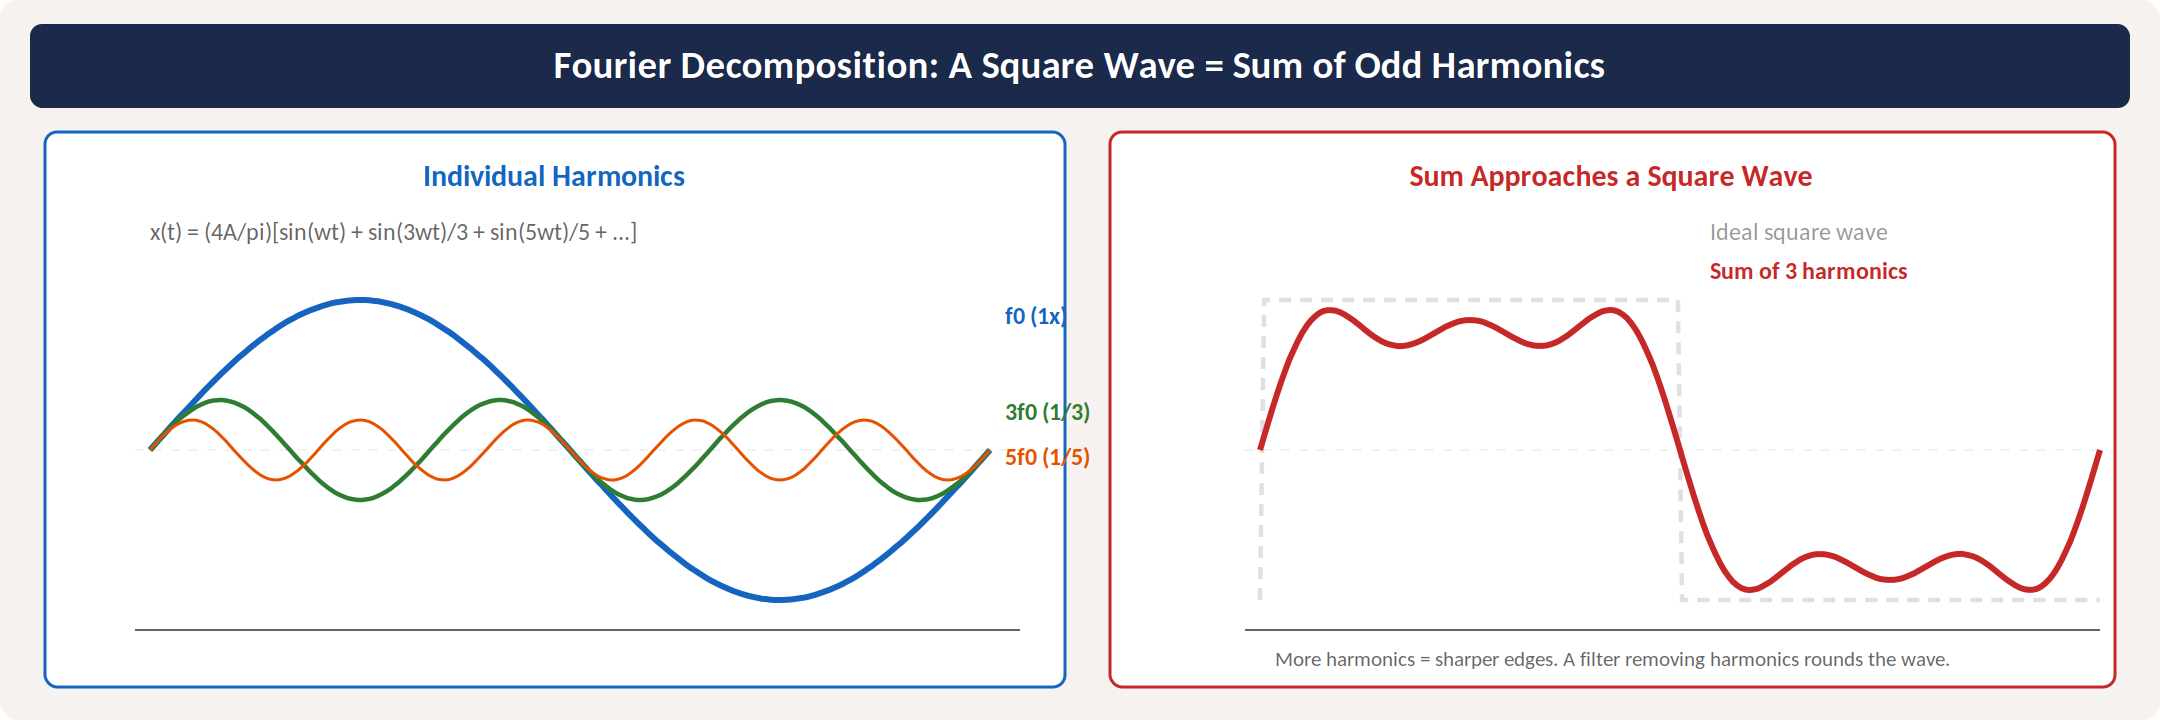
\includegraphics[width=\textwidth]{fig_fourier_decomposition.png}
\caption{Fourier decomposition of a square wave. Left: individual harmonics (fundamental, 3rd, 5th). Right: their sum approaches the square wave. Removing harmonics (e.g., with a low-pass filter) rounds the edges.}
\label{fig:fourier}
\end{figure}

\begin{tipbox}[Why Fourier Series Matters for Instrumentation]
Every real signal is a superposition of sinusoids. If your measurement system attenuates or phase-shifts any frequency component differently from others, the reconstructed signal is distorted. Understanding Fourier decomposition lets you predict how your sensor's frequency response (Chapter~3) and your filters (Chapters~10--11) will affect the measured signal.
\end{tipbox}


\section{Why Frequency Matters in Instrumentation}
Every sensor, amplifier, filter, and ADC has a frequency-dependent response. To understand, predict, and design these behaviors, we need to describe signals in terms of frequency content. The Fourier series provides this: any periodic signal decomposes into sinusoids at harmonics of the fundamental frequency.

\section{Mathematical Foundation}
A periodic signal $x(t)$ with period $T$ and fundamental $f_0 = 1/T$:
\begin{equation}
x(t) = \frac{a_0}{2} + \sum_{n=1}^{\infty}\left[a_n\cos(2\pi n f_0 t) + b_n\sin(2\pi n f_0 t)\right]
\end{equation}
where $a_n = (2/T)\int_0^T x(t)\cos(2\pi n f_0 t)\,dt$ and $b_n = (2/T)\int_0^T x(t)\sin(2\pi n f_0 t)\,dt$. The amplitude of the $n$th harmonic is $c_n = \sqrt{a_n^2 + b_n^2}$.

\section{Common Waveforms}
\textbf{Square wave}: $x(t) = (4A/\pi)[\sin(\omega_0 t) + \sin(3\omega_0 t)/3 + \sin(5\omega_0 t)/5 + \cdots]$. Only odd harmonics, amplitudes $\propto 1/n$. Sharp edges require many harmonics.

\textbf{Triangle wave}: odd harmonics, amplitudes $\propto 1/n^2$. Converges faster because transitions are smooth.

\textbf{Sawtooth}: all harmonics, amplitudes $\propto 1/n$.

\section{Physical Interpretation}
A measurement system must pass all significant harmonics. A sensor measuring a 100\,Hz square wave must have bandwidth covering at least the 5th harmonic (500\,Hz) to avoid severe distortion. For faithful edge reproduction, the 11th harmonic (1100\,Hz) or higher is needed.

\section{The Gibbs Phenomenon}
Truncating the series near a discontinuity produces $\sim$9\% overshoot that narrows but never disappears with more terms. In instrumentation, this manifests as ``ringing'' when a filter truncates harmonics.

\section{From Series to Transform}
The Fourier series applies to periodic signals. The Fourier transform generalizes to non-periodic signals (transients, events) by letting the period approach infinity. The discrete version (DFT/FFT) is the computational tool used in digital systems (Chapter~8).

\begin{tipbox}[Parseval's Theorem]
Total signal energy is the same in time and frequency domains: $\sum|x[n]|^2 = (1/N)\sum|X[k]|^2$. A filter removing frequency components removes their energy. If noise is concentrated in a narrow band (e.g., 60\,Hz), a notch filter removes that energy without affecting the rest.
\end{tipbox}


\section{Complex Exponential Representation}
Euler's formula $e^{j\theta} = \cos\theta + j\sin\theta$ allows sine and cosine to be combined into a single complex exponential. The Fourier series in complex form:
\begin{equation}
x(t) = \sum_{n=-\infty}^{\infty} c_n \, e^{j2\pi n f_0 t}
\end{equation}
where $c_n = (1/T)\int_0^T x(t)e^{-j2\pi n f_0 t}\,dt$. Negative frequencies are mathematical conveniences representing the complex conjugate of positive frequencies. For real signals, $c_{-n} = c_n^*$.

\section{Convergence and the Dirichlet Conditions}
The Fourier series converges for any signal satisfying the Dirichlet conditions: (1) finitely many discontinuities per period, (2) finitely many maxima and minima per period, (3) absolutely integrable over one period. All physical signals satisfy these conditions.

\section{Practical Implications for Bandwidth Requirements}
To pass a square wave through a measurement system with less than 10\% distortion (measured by total harmonic distortion, THD), you must pass harmonics through the 7th ($7f_0$). For less than 5\%: through the 11th. For less than 1\%: through the 25th or higher. This directly determines the sensor and filter bandwidth requirements.

A 100\,Hz square wave with 5\% THD limit requires system bandwidth $\geq 1100$\,Hz. If your anti-alias filter cuts off at 500\,Hz, the 7th harmonic (700\,Hz) and above are removed, distorting the signal.

\section{Spectral Analysis of Real Signals}
Real instrumentation signals are never pure sinusoids. A motor vibration signal typically contains: the fundamental rotation frequency, harmonics from gear tooth meshing, bearing defect frequencies, and broadband noise from turbulence. Fourier analysis separates these into distinct spectral lines, enabling diagnosis. A peak at $f = N_{\text{teeth}} \times f_{\text{shaft}}$ identifies gear mesh; a peak at $0.4 \times f_{\text{shaft}}$ identifies a ball-bearing outer race defect.
\section{Why Engineers Must Think in Frequency}
Consider a vibrating beam. In the time domain, you see a complex, seemingly random oscillation. In the frequency domain, you see three sharp peaks: the first, second, and third natural frequencies at 15, 94, and 263\,Hz. Each peak corresponds to a mode shape. The frequency domain reveals the physics; the time domain obscures it.

This principle applies universally in instrumentation: noise has a spectrum (concentrated at 60\,Hz and its harmonics), sensor bandwidth is defined in frequency, filter design is frequency-domain engineering, and control system stability is analyzed in frequency. Fourier analysis is the bridge between the physical time-domain world and the engineering frequency-domain tools.

\section{Even and Odd Function Decomposition}
Any signal can be decomposed into an even part $x_e(t) = [x(t) + x(-t)]/2$ and an odd part $x_o(t) = [x(t) - x(-t)]/2$. The even part has only cosine terms in the Fourier series ($b_n = 0$); the odd part has only sine terms ($a_n = 0$). This simplifies computation: if you know a signal is symmetric about $t = 0$ (even), you only need to compute cosine coefficients. If anti-symmetric (odd), only sine coefficients.

\section{Power and Energy in the Frequency Domain}
The average power of a periodic signal can be computed from its Fourier coefficients (Parseval's theorem):
\begin{equation}
P = \frac{a_0^2}{4} + \frac{1}{2}\sum_{n=1}^{\infty}(a_n^2 + b_n^2) = c_0^2 + \frac{1}{2}\sum_{n=1}^{\infty}c_n^2
\end{equation}
This means the total power is the sum of the power in each harmonic. A useful metric: the fraction of total power contained in the first $N$ harmonics indicates how many harmonics are ``significant.'' For a square wave, 90\% of the power is in the first 3 harmonics ($f_0$, $3f_0$, $5f_0$). For a triangle wave, 98\% is in the first 3. This quantifies the bandwidth needed to capture the signal.

\section{Total Harmonic Distortion (THD)}
THD quantifies how much a system distorts a pure sine wave:
\begin{equation}
\text{THD} = \frac{\sqrt{c_2^2 + c_3^2 + c_4^2 + \cdots}}{c_1} \times 100\%
\end{equation}
where $c_1$ is the fundamental amplitude and $c_n$ are the harmonic amplitudes. A DAQ with 0.01\% THD introduces negligible distortion. A sensor or amplifier with 1\% THD generates significant harmonics that may be confused with real signal content. In vibration analysis, THD of the excitation source must be verified before using it for frequency response measurement.

\section{Modulation and Demodulation}
\textbf{Amplitude modulation (AM)}: a low-frequency signal (e.g., strain gauge bridge output at 10\,Hz) modulates the amplitude of a high-frequency carrier (e.g., 5\,kHz excitation). The spectrum of the AM signal contains the carrier at 5\,kHz and sidebands at 4990\,Hz and 5010\,Hz. Demodulation recovers the original 10\,Hz signal. Advantage: the signal is shifted to a frequency range where 1/f noise and DC drift are negligible.

\textbf{Frequency modulation (FM)}: the signal modulates the frequency of an oscillator. Used in voltage-to-frequency (VFC) converters for noise-immune data transmission over long cables. A 0--10\,V signal modulates a 10--100\,kHz oscillator. The receiver counts the frequency to recover the voltage.

\section{Discrete Fourier Series and the Transition to DFT}
When a computer processes sampled data, the continuous integrals of the Fourier series become discrete sums. For a periodic signal sampled at $N$ equally spaced points:
\begin{equation}
c_k = \frac{1}{N}\sum_{n=0}^{N-1} x[n]\,e^{-j2\pi kn/N}
\end{equation}
This is the Discrete Fourier Transform (DFT), covered in full in Chapter~8. The key insight: $N$ samples produce $N$ frequency coefficients, but only $N/2$ are unique (the other half are complex conjugates). The frequency spacing is $\Delta f = f_s/N$, and the maximum frequency is $f_s/2$.

\section{Windowing Preview}
The DFT assumes the $N$-point data block is one period of a periodic signal. If the signal is not exactly periodic in $N$ samples (which it almost never is in practice), the assumption is violated, and spectral leakage occurs. Chapter~8 discusses windowing functions that mitigate this problem. The Fourier series context here helps explain why: the discontinuity at the block boundary is a sharp transient, which the Fourier series represents as a superposition of many harmonics. The window eliminates the discontinuity.
\section{Fourier Transform of Common Signals}
While the Fourier series handles periodic signals, many instrumentation signals are non-periodic. The Fourier transform extends the analysis:

\textbf{Impulse (Dirac delta)}: $\mathcal{F}\{\delta(t)\} = 1$ (flat spectrum, all frequencies equally present). An ideal impulse contains infinite bandwidth, which is why impact testing excites all resonances simultaneously.

\textbf{Rectangular pulse}: $\mathcal{F}\{\text{rect}(t/T)\} = T \cdot \text{sinc}(fT)$. The spectrum is a sinc function with first null at $f = 1/T$. A narrower pulse has a wider spectrum (more bandwidth).

\textbf{Exponential decay}: $\mathcal{F}\{e^{-t/\tau}u(t)\} = \tau/(1+j2\pi f\tau)$. This is the impulse response of a first-order system, confirming that the frequency response is $1/\sqrt{1+(\omega\tau)^2}$.

\textbf{Gaussian pulse}: $\mathcal{F}\{e^{-t^2/(2\sigma^2)}\} = \sigma\sqrt{2\pi} \cdot e^{-2(\pi f\sigma)^2}$. A Gaussian in time has a Gaussian spectrum. The ``uncertainty principle'': the product of the time-domain width and frequency-domain width is constant. Narrower in time = wider in frequency. This is a fundamental constraint on simultaneous time and frequency resolution.

\section{The Short-Time Fourier Transform (STFT) and Spectrograms}
The standard FFT computes the frequency content over the entire signal duration. For signals whose frequency content changes with time (motor speed ramp-up, earthquake, speech), the \textbf{Short-Time Fourier Transform} divides the signal into overlapping segments, computes the FFT of each, and displays the result as a time-frequency map called a \textbf{spectrogram} (or waterfall plot).

In LabVIEW, the ``STFT Spectrogram'' VI computes this. Parameters: segment length (determines frequency resolution), overlap (typically 75\%), and window function (Hanning). The spectrogram is invaluable for analyzing run-up/coast-down vibration tests, transient thermal events, and any measurement where the frequency content evolves over time.
\section{Bandwidth and Harmonic Content: A Design Tool}
The Fourier series provides a quantitative tool for determining the bandwidth needed to faithfully reproduce a given waveform. The key metric: how many harmonics must be preserved to keep the waveform distortion below a specified threshold?

Define the harmonic energy fraction: $E_N / E_{\text{total}} = \sum_{n=1}^{N} c_n^2 / \sum_{n=1}^{\infty} c_n^2$.

For a square wave: $E_1/E_{\text{total}} = 81\%$ (fundamental alone). $E_3/E_{\text{total}} = 90\%$ (through 3rd harmonic). $E_5/E_{\text{total}} = 93.4\%$. $E_{11}/E_{\text{total}} = 97\%$. So passing harmonics through the 11th captures 97\% of the energy. For a 100\,Hz square wave: the measurement system needs bandwidth of at least $11 \times 100 = 1100$\,Hz.

For a triangle wave: $E_1 = 97\%$, $E_3 = 98.8\%$. The triangle wave is nearly sinusoidal; bandwidth of $3f_0$ captures 99\% of the energy. This is why triangle waves pass through narrow-bandwidth systems with minimal distortion, while square waves are heavily distorted.

For a half-sine pulse (rectified sine): contains even harmonics. $E_2/E_{\text{total}} = 95\%$. Bandwidth of $2f_0$ is nearly sufficient.

\section{Fourier Series in Sensor Design}
Sensor designers use Fourier analysis to specify bandwidth requirements. Example: a load cell measuring the force from a stamping press. The force waveform is approximately trapezoidal: a fast rise (impact), a flat peak (hold), and a fast fall (release). The trapezoidal waveform has harmonics decaying as $1/(n^2)$ times a sinc envelope. The bandwidth needed depends on the rise time $t_r$: $BW \geq 0.35/t_r$. For $t_r = 1$\,ms: $BW \geq 350$\,Hz. For $t_r = 0.1$\,ms (high-speed press): $BW \geq 3.5$\,kHz.

\section{Spectral Analysis in Troubleshooting}
When a measurement produces unexpected results, computing the Fourier series (or FFT) of the output often reveals the cause:

\textbf{Symptom}: temperature reading fluctuates $\pm$0.5\,\degC{} when the heater is off. \textbf{FFT}: sharp peak at 60\,Hz. \textbf{Diagnosis}: mains coupling. \textbf{Fix}: shielding + differential input.

\textbf{Symptom}: strain gauge reading drifts slowly over 30 minutes. \textbf{FFT}: 1/f-shaped spectrum (power increasing at low frequencies). \textbf{Diagnosis}: thermal drift in the bridge or amplifier. \textbf{Fix}: temperature-compensated half-bridge, or zero-drift amplifier.

\textbf{Symptom}: accelerometer output has a persistent component at exactly 2$\times$ shaft speed. \textbf{FFT}: peak at $2f_{\text{shaft}}$. \textbf{Diagnosis}: misalignment (classic signature). \textbf{Fix}: realign the coupling.

\textbf{Symptom}: pressure sensor output has a ``haystack'' (broad hump) centered at 200\,Hz. \textbf{FFT}: broad peak from 150--250\,Hz. \textbf{Diagnosis}: turbulent flow noise. \textbf{Fix}: cannot eliminate (physical phenomenon); increase signal averaging to reduce its effect on mean pressure measurement.
\section{Fourier Series Symmetry Properties}
Understanding symmetry simplifies Fourier analysis and provides physical insight:

\textbf{Even functions} ($x(t) = x(-t)$, symmetric about $t = 0$): contain only cosine terms ($b_n = 0$). Examples: cosine waves, rectified sine waves, any waveform that is a mirror image about $t = 0$.

\textbf{Odd functions} ($x(-t) = -x(t)$, anti-symmetric): contain only sine terms ($a_n = 0$, $a_0 = 0$). Examples: sine waves, square waves centered at zero, sawtooth waves.

\textbf{Half-wave symmetry} ($x(t + T/2) = -x(t)$): contains only odd harmonics ($a_n = b_n = 0$ for even $n$). The square wave, triangle wave, and any waveform where the second half-period is the negative of the first have this property.

These symmetry properties explain why the square wave contains only odd harmonics (it has half-wave symmetry), while the sawtooth contains all harmonics (it does not have half-wave symmetry).

\section{Convergence Rate and Bandwidth Implications}
The rate at which Fourier coefficients decrease with harmonic number $n$ is directly related to the smoothness of the waveform:

\textbf{Discontinuous waveform} (square wave): $c_n \propto 1/n$. Coefficients decay slowly. Many harmonics needed for faithful reproduction. Bandwidth requirement: $\sim 11f_0$ for 97\% energy capture.

\textbf{Continuous but with discontinuous derivative} (triangle wave): $c_n \propto 1/n^2$. Faster decay. Bandwidth: $\sim 3f_0$ for 99\% energy.

\textbf{Smooth waveform with continuous first derivative}: $c_n \propto 1/n^3$ or faster. Very few harmonics needed.

\textbf{Sinusoid}: $c_1 = A/2$, all other $c_n = 0$. Zero bandwidth beyond $f_0$.

The general rule: each additional order of continuity (smoothness) in the waveform adds a factor of $1/n$ to the coefficient decay rate. This is why digital signals (sharp edges, discontinuities) require much wider bandwidth than analog signals (smooth, continuous).

\section{Fourier Analysis of Real Sensor Signals}
\subsection{Vibration Signature Analysis}
A rotating machine produces a vibration signal that is periodic at the rotation frequency $f_r$ but not sinusoidal. The Fourier series reveals the harmonic structure:

$1 \times f_r$ (fundamental): unbalance. Amplitude indicates the severity of mass imbalance.

$2 \times f_r$: misalignment (angular or parallel). Often the dominant component in poorly aligned machinery.

$3 \times f_r$: looseness or rubbing. Indicates mechanical clearance problems.

$N_{\text{teeth}} \times f_r$: gear mesh frequency. Sidebands spaced at $f_r$ around the mesh peak indicate gear wear.

$N_{\text{blades}} \times f_r$: blade pass frequency in fans, pumps, and turbines.

The Fourier series connects the physical defect to its spectral signature, enabling condition-based maintenance.

\subsection{Electrical Power Quality}
The AC mains voltage is nominally a 60\,Hz (or 50\,Hz) sinusoid. Nonlinear loads (computers, LED drivers, variable-frequency drives) draw current in pulses, distorting the voltage waveform. The Fourier series quantifies this distortion:

Total Harmonic Distortion: $\text{THD} = \sqrt{c_2^2 + c_3^2 + \cdots}/c_1$. IEEE~519 limits THD to $< 5\%$ at the point of common coupling. A THD of 10\% indicates significant distortion that can cause overheating in transformers and interference in sensitive instrumentation.

The 3rd harmonic (180\,Hz) is typically the largest for single-phase nonlinear loads. In three-phase systems, the 3rd harmonic currents from each phase add constructively in the neutral conductor, potentially overloading it. The 5th (300\,Hz) and 7th (420\,Hz) harmonics are dominant for three-phase variable-frequency drives.

\section{Window Functions: Mathematical Basis}
The DFT assumes periodicity: the $N$-point data block is treated as one period of an infinitely repeating signal. If the actual signal is not periodic within the window, the implicit discontinuity at the block boundaries creates spectral leakage.

A window function $w[n]$ tapers the data to zero at both ends, eliminating the discontinuity. The price: the main lobe of each spectral line widens (reducing frequency resolution). The tradeoff between main lobe width and sidelobe level is characterized by:

\textbf{Main lobe width} (in bins): determines the minimum separation between two frequencies that can be resolved. Rectangular: 2 bins. Hanning: 4 bins. Flat-top: 8 bins. Blackman-Harris: 8 bins.

\textbf{Highest sidelobe level}: determines the dynamic range (ability to detect a small signal near a large one). Rectangular: $-13$\,dB. Hanning: $-31$\,dB. Flat-top: $-44$\,dB. Blackman-Harris: $-92$\,dB.

\textbf{Amplitude accuracy}: the error in measuring the amplitude of a spectral line that falls between bins. Rectangular: $-3.9$\,dB worst case. Hanning: $-1.4$\,dB. Flat-top: $-0.01$\,dB.
\section{Practical Frequency Analysis Workflow}
A systematic approach to analyzing the frequency content of measured signals:

\textbf{Step 1: Inspect the time-domain waveform.} Look for periodicity, transients, trends, and obvious anomalies. Estimate the dominant frequency visually (count cycles per unit time). Check for clipping (flat-topped peaks indicating ADC saturation).

\textbf{Step 2: Remove the mean.} Subtract the DC component before computing the spectrum. A large DC component produces a tall spike at bin 0 that can mask nearby low-frequency content. In LabVIEW: subtract the mean of the array before wiring to the FFT function.

\textbf{Step 3: Apply a window.} Select based on the application: Hanning for general analysis, Flat-top for amplitude measurement, Blackman-Harris for detecting small signals near large ones.

\textbf{Step 4: Compute the FFT and display.} Plot the magnitude spectrum in dB (not linear): $\text{dB} = 20\log_{10}(|X[k]|)$. The dB scale reveals both large and small components simultaneously. A linear scale shows only the dominant peaks.

\textbf{Step 5: Identify components.} Discrete peaks: identify the source (rotation speed, mains frequency, switching noise). Harmonics: verify they are integer multiples of a fundamental. Broadband noise: measure the PSD level in the flat regions.

\textbf{Step 6: Validate.} Change the acquisition parameters (different $f_s$, different $N$) and verify that the identified components do not shift frequency (which would indicate aliasing). If a peak at 200\,Hz moves to 300\,Hz when you change $f_s$: it is an alias, not a real signal.

\section{The Uncertainty Principle for Signals}
The product of time resolution and frequency resolution has a fundamental lower bound:
\begin{equation}
\Delta t \cdot \Delta f \geq \frac{1}{4\pi} \approx 0.08
\end{equation}
In practice, the achievable product is $\Delta t \cdot \Delta f \approx 1$ for most window functions. This means: to resolve 1\,Hz frequency difference ($\Delta f = 1$\,Hz), you need at least 1 second of data ($\Delta t \geq 1$\,s). To resolve events lasting 1\,ms ($\Delta t = 0.001$\,s), the best achievable frequency resolution is $\Delta f \geq 1000$\,Hz.

This tradeoff is not a limitation of the FFT algorithm; it is a fundamental property of signals. No analysis technique, no matter how sophisticated, can simultaneously achieve arbitrary time and frequency resolution.

\section{Hilbert Transform and Envelope Analysis}
The \textbf{Hilbert transform} produces the analytic signal $z(t) = x(t) + j\hat{x}(t)$, where $\hat{x}(t)$ is the Hilbert transform of $x(t)$. The magnitude $|z(t)|$ is the \textbf{envelope} (instantaneous amplitude) and $\angle z(t)$ is the instantaneous phase. The time derivative of the instantaneous phase gives the instantaneous frequency.

In vibration analysis, envelope analysis detects amplitude-modulated signals produced by bearing defects. The bearing defect produces a periodic impulse train (at the defect frequency) that amplitude-modulates the bearing's natural frequency (typically 2--5\,kHz). The envelope of the high-pass-filtered signal reveals the defect frequency, which is invisible in the raw spectrum (because it appears as sidebands, not a direct peak).
\section{Practice Questions}
\begin{enumerate}[leftmargin=1.5em]
\item A 100\,Hz square wave passes through a first-order low-pass filter with a 500\,Hz cutoff. What happens to the fundamental and the first four odd harmonics (100, 300, 500, 700, 900\,Hz)? Describe the distortion qualitatively.
\item A signal has a fundamental at 50\,Hz and significant harmonic content at 150\,Hz and 250\,Hz. What is the minimum sampling rate to capture all three components without aliasing?
\item Write the first three nonzero terms of the Fourier series for a triangle wave with amplitude 2\,V and frequency 1\,kHz.
\end{enumerate}

\subsection{Answers}
\begin{enumerate}[leftmargin=1.5em]
\item At 100\,Hz: $M = 1/\sqrt{1+(100/500)^2} = 0.981$ (nearly passed). At 300\,Hz: $M = 0.857$. At 500\,Hz: $M = 0.707$ ($-3$\,dB point). At 700\,Hz: $M = 0.581$. At 900\,Hz: $M = 0.486$. The higher harmonics that define the sharp edges of the square wave are progressively attenuated; the output will look like a rounded square wave with slower rise/fall times.
\item Nyquist: $f_s > 2 \times f_{\max} = 2 \times 250 = 500$\,Hz minimum. In practice, use $f_s \geq 2.5 \times 250 = 625$\,Hz or higher.
\item Triangle wave: $x(t) = \frac{8A}{\pi^2}\left[\sin(2\pi f_0 t) - \frac{1}{9}\sin(6\pi f_0 t) + \frac{1}{25}\sin(10\pi f_0 t) - \cdots\right]$. With $A = 2$\,V, $f_0 = 1000$\,Hz: $x(t) = \frac{16}{\pi^2}\left[\sin(2000\pi t) - \frac{1}{9}\sin(6000\pi t) + \frac{1}{25}\sin(10000\pi t)\right] \approx 1.621\sin(2000\pi t) - 0.180\sin(6000\pi t) + 0.065\sin(10000\pi t)$.
\end{enumerate}


% ================================================================
\chapter{FFT and Complex Signal Decomposition}

\section{From Fourier Series to Fourier Transform}
The Fourier series applies to periodic signals. For non-periodic or finite-duration signals, the \textbf{Fourier Transform} generalizes the concept to a continuous frequency spectrum:
\begin{equation}
X(f) = \int_{-\infty}^{\infty} x(t) \, e^{-j2\pi f t} \, dt
\end{equation}
$X(f)$ is complex-valued: its magnitude $|X(f)|$ gives the amplitude spectrum, and its angle $\angle X(f)$ gives the phase spectrum.

\section{The Discrete Fourier Transform (DFT) and FFT}
For sampled data ($N$ points, sampling rate $f_s$), the DFT computes:
\begin{equation}
X[k] = \sum_{n=0}^{N-1} x[n] \, e^{-j2\pi kn/N}, \quad k = 0, 1, \ldots, N-1
\end{equation}
The \textbf{Fast Fourier Transform (FFT)} is an algorithm that computes the DFT in $O(N \log N)$ operations instead of $O(N^2)$. For $N = 1024$: DFT requires $\sim$1 million multiplications; FFT requires $\sim$10,000. This is what makes real-time spectral analysis practical.

\subsection{Interpreting the FFT Output}
The FFT produces $N$ complex numbers. The useful frequency range is $0$ to $f_s/2$ (first $N/2 + 1$ bins). The frequency resolution (bin width) is:
\begin{equation}
\Delta f = \frac{f_s}{N}
\end{equation}
To resolve two closely spaced frequencies, you need $\Delta f$ smaller than their separation. Increasing $N$ (longer acquisition time) improves frequency resolution.

\subsection{Windowing}
The FFT assumes the signal is periodic within the acquisition window. If the signal frequency does not exactly match an FFT bin, the result ``leaks'' energy into adjacent bins (\textbf{spectral leakage}). Windowing functions (Hanning, Hamming, Blackman, flat-top) taper the signal edges to reduce leakage at the cost of slightly reduced frequency resolution.

\begin{tipbox}[Which Window to Use]
Hanning (Hann): best general-purpose choice; good frequency resolution with moderate leakage. Flat-top: best for accurate amplitude measurement of known tones. Rectangular (no window): best frequency resolution but worst leakage; use only when the signal is exactly periodic in the window.
\end{tipbox}

\begin{figure}[htbp]
\centering
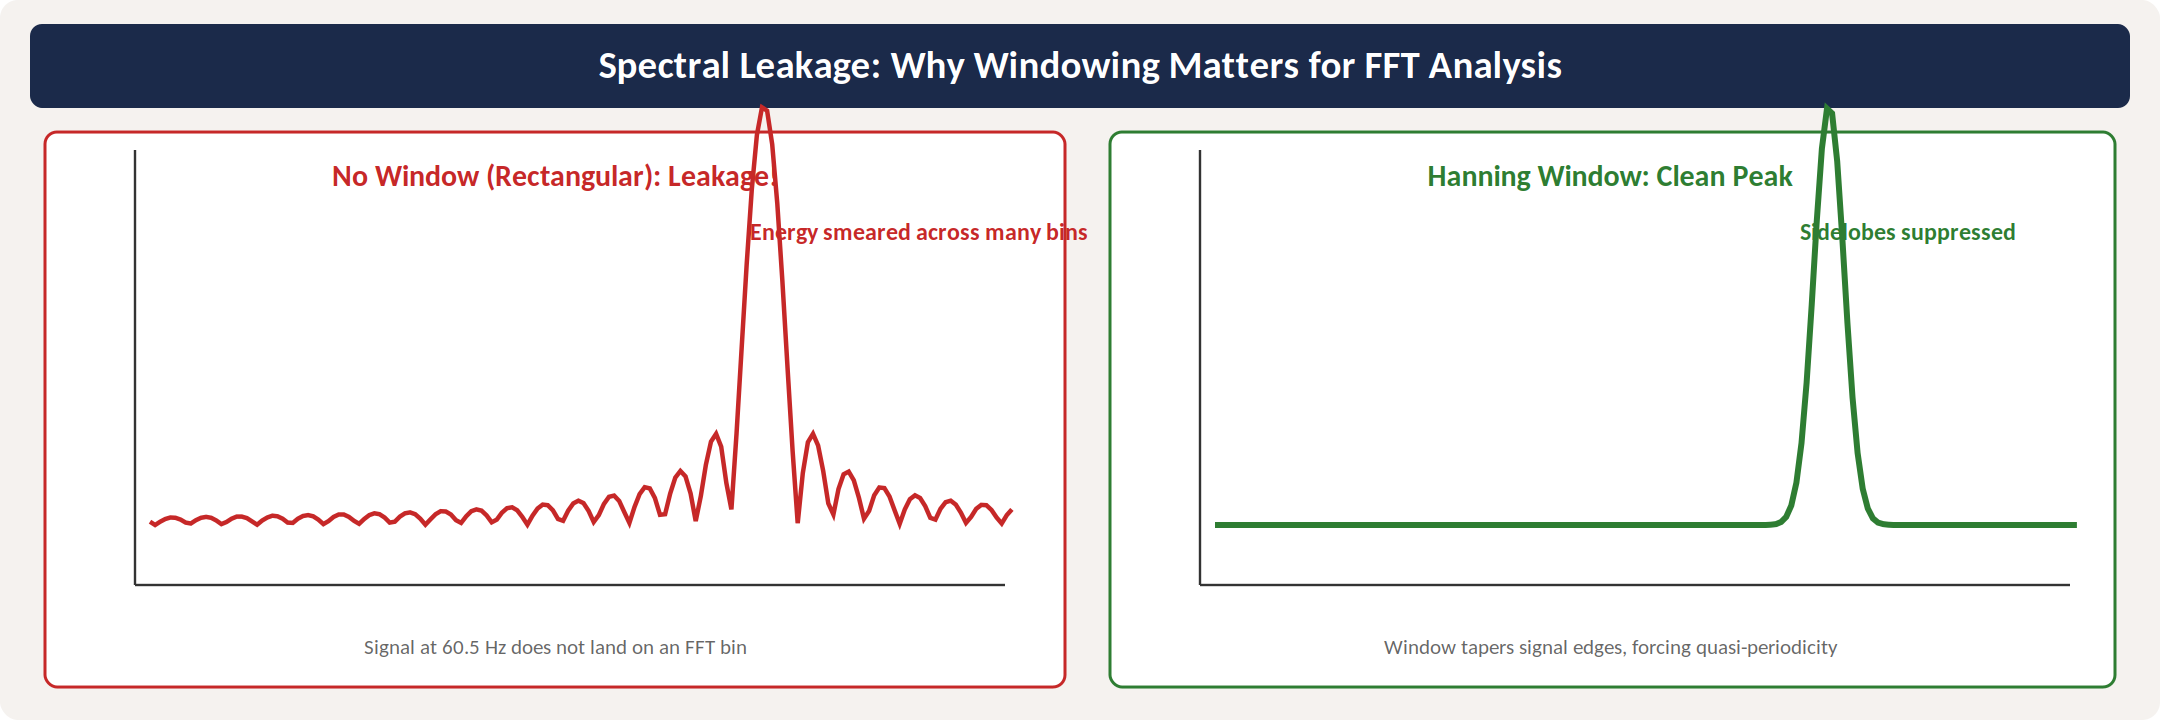
\includegraphics[width=\textwidth]{fig_spectral_leakage.png}
\caption{Spectral leakage: without windowing (left), a 60.5\,Hz signal that does not land on an FFT bin smears across many bins. With a Hanning window (right), the energy concentrates into a narrow peak. Always window unless the signal is exactly periodic in the acquisition window.}
\label{fig:leakage}
\end{figure}

\section{Practical FFT in LabVIEW}
In LabVIEW, use the \texttt{FFT Power Spectrum and PSD} VI. Set: $N$ (power of 2 for efficiency), window type, and averaging mode. The output is a 1D array of power spectral density (PSD) values in $\text{V}^2/\text{Hz}$ or amplitude spectrum in V\textsubscript{RMS}.


\section{Power Spectral Density (PSD)}
The PSD describes how the signal's power is distributed across frequencies, normalized by the frequency resolution:
\begin{equation}
\text{PSD}(f) = \frac{|X(f)|^2}{N \cdot f_s} \quad [\text{V}^2/\text{Hz}]
\end{equation}
PSD is independent of the FFT length $N$ and sampling rate $f_s$, making it suitable for comparing measurements taken with different acquisition parameters. Use PSD for broadband (continuous) signals like vibration and noise. Use amplitude spectrum for discrete tones (known frequencies).

\section{Averaging for Spectral Estimates}
A single FFT of noisy data has high variance. Averaging reduces this variance:

\textbf{Linear averaging}: divide the signal into $M$ overlapping segments, compute the FFT of each, and average the magnitude spectra. Reduces spectral variance by $1/M$. Use 50\% overlap with Hanning window for optimal noise reduction with minimal data loss.

\textbf{Exponential averaging}: weights recent FFTs more heavily; tracks slowly changing spectra. Set the averaging constant based on how quickly the spectrum changes.

\section{Practical FFT Analysis Workflow}
\begin{enumerate}[leftmargin=1.5em]
\item Choose $f_s \geq 2.56 \times f_{\max}$ (signal bandwidth + anti-alias margin).
\item Choose $N$ based on required frequency resolution: $N = f_s / \Delta f$. Use a power of 2.
\item Apply a window function (Hanning for general use).
\item Compute the FFT; convert to single-sided amplitude or PSD.
\item Average multiple blocks (10--100 averages for noisy data).
\item Identify peaks; read frequency and amplitude. Compare to noise floor.
\end{enumerate}


\section{From DFT to FFT}
The Discrete Fourier Transform (DFT) computes the frequency content of a sampled signal by decomposing it into $N$ complex sinusoids:
\begin{equation}
X[k] = \sum_{n=0}^{N-1} x[n] \, e^{-j2\pi kn/N}, \quad k = 0, 1, \ldots, N-1
\end{equation}
where $x[n]$ is the $n$th time-domain sample and $X[k]$ is the complex amplitude at frequency $f_k = k \cdot f_s / N$. Computing the DFT directly requires $N^2$ complex multiplications. The \textbf{Fast Fourier Transform (FFT)} is an algorithm (Cooley-Tukey, 1965) that reduces this to $N \log_2 N$ operations by exploiting symmetry and periodicity. For $N = 1024$, this is a 100$\times$ speedup; for $N = 1{,}048{,}576$ (one million points), it is a 50{,}000$\times$ speedup.

\section{FFT Output Interpretation}
The FFT output $X[k]$ is a complex number with magnitude and phase. The \textbf{magnitude spectrum} $|X[k]|$ shows how much of each frequency is present. The \textbf{phase spectrum} $\angle X[k]$ shows the phase angle of each frequency component. In LabVIEW, the ``FFT'' function returns both; the ``Power Spectrum'' function returns $|X[k]|^2/N$ or its variants.

\subsection{Frequency Resolution}
The spacing between adjacent frequency bins is:
\begin{equation}
\Delta f = \frac{f_s}{N}
\end{equation}
To resolve two closely spaced frequencies (e.g., 99\,Hz and 101\,Hz, $\Delta f = 2$\,Hz), you need $N \geq f_s / \Delta f$. At $f_s = 1000$\,S/s, this requires $N \geq 500$ samples (0.5\,s of data). Want 0.1\,Hz resolution? You need $N = 10{,}000$ samples (10\,s of data at 1\,kS/s). This is the fundamental tradeoff: \textbf{better frequency resolution requires longer acquisition time}.

\subsection{Frequency Range}
The FFT produces output from $f = 0$ (DC) to $f = f_s/2$ (Nyquist). Only the first $N/2$ bins are unique; the second half is a mirror image (for real-valued input signals). In practice, you use bins $k = 0$ to $k = N/2$.

\section{Power Spectral Density (PSD)}
For random or broadband signals, the magnitude spectrum depends on the FFT length $N$ (longer records produce taller peaks because more energy is captured). The \textbf{Power Spectral Density (PSD)} normalizes by the frequency resolution:
\begin{equation}
\text{PSD}[k] = \frac{|X[k]|^2}{N \cdot \Delta f} \quad \text{(units: V$^2$/Hz)}
\end{equation}
The PSD is independent of record length, making it the correct representation for comparing noise floors, characterizing random vibration, and specifying sensor noise performance.

\section{Windowing: Theory and Practice}
The FFT assumes the signal is exactly periodic within the acquisition window of $N$ samples. If this assumption is violated (which it almost always is for real signals), the resulting discontinuity at the window boundaries produces \textbf{spectral leakage}: the energy of a single frequency smears across adjacent bins, reducing amplitude accuracy and frequency resolution.

\subsection{The Root Cause}
Consider acquiring 1000 samples of a 100.5\,Hz sine wave at 1000\,S/s. The FFT frequency bins are at 0, 1, 2, $\ldots$, 999\,Hz (with 1\,Hz spacing). The signal frequency (100.5\,Hz) falls between bins 100 and 101. The FFT cannot represent 100.5\,Hz exactly, so the energy ``leaks'' into neighboring bins, producing a smeared peak with sidelobes.

\subsection{Window Functions}
A window function $w[n]$ is multiplied with the signal before the FFT: $x_w[n] = x[n] \cdot w[n]$. The window tapers the signal to zero at both ends, forcing it to appear periodic and reducing the discontinuity. Common windows and their tradeoffs:

\textbf{Rectangular (no window)}: highest frequency resolution (narrowest main lobe) but worst sidelobe rejection ($-13$\,dB). Use only when the signal is exactly periodic in the window.

\textbf{Hanning}: moderate resolution, good sidelobe rejection ($-31$\,dB). The default choice for general-purpose spectral analysis.

\textbf{Flat-top}: wide main lobe (poor frequency resolution) but extremely accurate amplitude measurement ($<$0.01\,dB error). Use when you need to measure the exact amplitude of a known frequency (e.g., calibration).

\textbf{Blackman-Harris}: excellent sidelobe rejection ($-92$\,dB) but widest main lobe. Use when small signals near large ones must be detected.

\begin{examplebox}[ThermoRig: Identifying Switching Noise with FFT]
The ThermoRig thermocouple signal, sampled at 10\,kS/s ($N = 8192$ for FFT), reveals a sharp peak at 60\,Hz (expected: mains coupling) and a broader peak near 500\,kHz that has been aliased to 0.5\,kHz. This aliased component comes from the switching regulator's 500\,kHz oscillator, which couples capacitively into the thermocouple wiring. The Hanning window produces clean, narrow peaks at both frequencies, confirming they are discrete tones rather than broadband noise. The solution: add a 100\,Hz anti-alias filter before the ADC, eliminating the aliased component entirely.
\end{examplebox}

\section{Spectral Averaging}
A single FFT of a random (noisy) signal produces a noisy spectrum. To obtain a smooth estimate of the PSD, compute multiple FFTs of successive blocks of data and average the magnitude spectra. With $M$ averages, the variance of the PSD estimate decreases by a factor of $M$. Typical practice: 10--100 averages for laboratory measurements, 100--1000 for production testing.

\subsection{Overlap Processing}
To improve the effective averaging rate without acquiring more data, successive FFT blocks can overlap (typically 50--75\%). With 50\% overlap, a Hanning-windowed signal uses approximately 90\% of the acquired data (vs.\ 50\% without overlap). LabVIEW's ``Power Spectrum'' function supports overlap processing natively.

\section{Common FFT Pitfalls}
\begin{enumerate}[leftmargin=1.5em]
\item \textbf{Forgetting the anti-alias filter}: aliased components appear real and cannot be distinguished from true signals in the FFT.
\item \textbf{Not windowing}: spectral leakage smears energy across bins, reducing dynamic range.
\item \textbf{Using too few points}: poor frequency resolution causes adjacent peaks to merge.
\item \textbf{Confusing linear and dB scales}: a peak at $-40$\,dB is not ``almost zero''; it is 1\% of full scale.
\item \textbf{Ignoring DC offset}: a large DC component (bin 0) can mask nearby low-frequency content. Remove the mean before computing the FFT.
\end{enumerate}


\section{From DFT to FFT}
The DFT: $X[k] = \sum_{n=0}^{N-1} x[n]\,e^{-j2\pi kn/N}$, $k = 0,\ldots,N-1$. Direct computation: $O(N^2)$. The FFT (Cooley-Tukey, 1965) reduces this to $O(N\log_2 N)$. For $N = 1024$: 100$\times$ speedup. For $N = 10^6$: 50,000$\times$.

\section{FFT Output Interpretation}
$X[k]$ is complex: magnitude $|X[k]|$ gives amplitude at frequency $f_k = k \cdot f_s/N$; phase $\angle X[k]$ gives the phase angle. Only bins $k = 0$ to $N/2$ are unique for real input.

\textbf{Frequency resolution}: $\Delta f = f_s/N$. To resolve 99\,Hz from 101\,Hz ($\Delta f = 2$\,Hz) at 1\,kS/s requires $N \geq 500$ (0.5\,s of data). Better resolution requires longer acquisition.

\section{Power Spectral Density}
For random signals, the magnitude spectrum depends on $N$. The PSD normalizes: $\text{PSD}[k] = |X[k]|^2/(N\cdot\Delta f)$ (units: V$^2$/Hz). PSD is independent of record length, making it the correct representation for noise characterization.

\section{Windowing}
The FFT assumes the signal is periodic within the window. Non-periodic signals create discontinuities at the window edges, causing spectral leakage. A window function tapers the signal to zero at both ends.

\textbf{Rectangular}: best resolution, worst sidelobes ($-13$\,dB). Use only for exactly periodic signals.

\textbf{Hanning}: good general-purpose choice. $-31$\,dB sidelobes.

\textbf{Flat-top}: wide main lobe but $<$0.01\,dB amplitude error. Use for calibration.

\textbf{Blackman-Harris}: $-92$\,dB sidelobes. Use when small signals near large ones must be detected.

\section{Spectral Averaging and Overlap}
A single FFT of noisy data produces a noisy spectrum. Average $M$ FFTs to reduce variance by $M$. With 50\% overlap between successive blocks, approximately 90\% of data is used. LabVIEW's Power Spectrum supports overlap processing natively.

\begin{examplebox}[ThermoRig: Identifying Switching Noise]
FFT of TC signal at 10\,kS/s ($N = 8192$) reveals: 60\,Hz peak (mains coupling) and 500\,Hz peak (aliased 500\,kHz switching regulator). Hanning window confirms both are discrete tones. Fix: 100\,Hz anti-alias filter eliminates the aliased component.
\end{examplebox}

\section{Common FFT Pitfalls}
(1) Forgetting anti-alias filter: aliases look real. (2) Not windowing: leakage smears peaks. (3) Too few points: poor resolution. (4) Confusing linear and dB scales: $-40$\,dB is 1\%, not ``almost zero.'' (5) Large DC offset masks low-frequency content; remove mean before FFT.


\section{Choosing FFT Parameters for MEGN 300 Labs}
When setting up an FFT measurement in LabVIEW, four parameters must be chosen correctly:

\textbf{Sample rate $f_s$}: must be at least $2.56\times$ the highest frequency of interest (standard vibration analysis convention). For a 1\,kHz bandwidth measurement: $f_s \geq 2560$\,S/s. Round up to a convenient value (4096\,S/s or 5000\,S/s).

\textbf{Number of points $N$}: determines frequency resolution ($\Delta f = f_s/N$). For 1\,Hz resolution at 4096\,S/s: $N \geq 4096$. For 0.1\,Hz resolution: $N \geq 40{,}960$. $N$ should be a power of 2 for maximum FFT algorithm efficiency (1024, 2048, 4096, 8192, etc.).

\textbf{Window function}: Hanning is the default for general use. Use Flat-top when amplitude accuracy is critical (calibration, amplitude comparison). Use Rectangular only when the signal is exactly periodic in the window (e.g., a frequency generator locked to the DAQ clock).

\textbf{Number of averages}: for random/noisy signals, average 10--100 spectra to reduce variance. For deterministic signals (sine waves, harmonics), a single FFT is sufficient.

\subsection{Acquisition Time Tradeoff}
The total acquisition time is $T = N \times M / f_s$ where $M$ is the number of averages. For $f_s = 4096$\,S/s, $N = 4096$, $M = 50$ averages with 50\% overlap: $T \approx 25.6$\,s. Finer frequency resolution or more averaging requires longer acquisition. Plan accordingly for time-limited measurements.

\section{Interpreting FFT Results}
\subsection{Identifying Signal Components}
\textbf{Discrete tones}: sharp, narrow peaks at specific frequencies. Sources: rotating machinery (shaft speed and harmonics), electrical interference (60\,Hz, switching frequencies), resonances (structural natural frequencies). The peak height gives the amplitude; the peak frequency identifies the source.

\textbf{Broadband noise}: a raised floor across many or all frequencies. Sources: thermal noise, turbulent flow, friction. The PSD level (V$^2$/Hz) characterizes the noise intensity.

\textbf{Sidebands}: peaks flanking a main peak, spaced equally on both sides. Sources: amplitude modulation (bearing defects modulating shaft rotation), frequency modulation (speed fluctuations). The sideband spacing identifies the modulation frequency.

\subsection{Frequency Identification Guide}
For a machine rotating at $f_r$: shaft imbalance appears at $f_r$. Misalignment at $2f_r$. Gear mesh at $N_{\text{teeth}} \times f_r$. Ball bearing outer race defect at $\sim 0.4 N_{\text{balls}} \times f_r$. Blade pass frequency at $N_{\text{blades}} \times f_r$. Electrical motor slip frequency at $(f_{\text{line}} - N_p f_r)$ where $N_p$ is the number of poles.

\section{Cross-Spectral Analysis}
When measuring two channels simultaneously (e.g., force input and acceleration output), the \textbf{cross-spectrum} $G_{xy}(f) = X^*(f) \cdot Y(f)$ relates the two signals in the frequency domain. The \textbf{frequency response function} (transfer function magnitude) is:
\begin{equation}
|H(f)| = \frac{|G_{xy}(f)|}{G_{xx}(f)}
\end{equation}
where $G_{xx}$ is the auto-spectrum of the input. The \textbf{coherence function} $\gamma^2(f) = |G_{xy}|^2/(G_{xx} G_{yy})$ indicates how much of the output is linearly related to the input at each frequency. $\gamma^2 = 1$: output is completely explained by the input. $\gamma^2 < 0.9$: other sources (noise, nonlinearity, unmeasured inputs) contribute significantly.

\section{Practical LabVIEW FFT Implementation}
The recommended LabVIEW approach for FFT measurement:

(1) Use the ``Spectral Measurements'' Express VI for simple measurements (magnitude, phase, PSD). It handles windowing, averaging, and scaling automatically.

(2) For more control, use the ``FFT'' primitive: wire in the time-domain waveform, apply a window (``Scaled Time Domain Window'' VI), compute the FFT, take the magnitude, and scale appropriately.

(3) For real-time display, place the FFT inside a While Loop with a ``Waveform Chart'' or ``Intensity Graph'' for waterfall (spectrogram) display. The spectrogram shows how the frequency content evolves over time, which is invaluable for diagnosing transient events and speed-varying machinery.
\section{FFT Resolution Enhancement Techniques}
\subsection{Zero-Padding}
Appending zeros to the time-domain data before computing the FFT increases the number of frequency bins without acquiring more data. Zero-padding does \emph{not} improve the true frequency resolution (which is fixed at $\Delta f = 1/T_{\text{acq}}$ where $T_{\text{acq}}$ is the acquisition duration), but it interpolates between the existing bins, producing a smoother spectrum that makes it easier to identify peak frequencies.

For example: 1024 samples at 1\,kS/s gives $\Delta f = 1$\,Hz with 512 frequency bins. Zero-padding to 4096 points gives the same $\Delta f = 1$\,Hz resolution but now with 2048 bins (interpolated), making peaks easier to locate visually.

\subsection{Zoom FFT}
To achieve very fine frequency resolution in a narrow band without acquiring an impractically long record: (1) frequency-shift the band of interest to baseband by multiplying the signal by $e^{-j2\pi f_c t}$ where $f_c$ is the center frequency, (2) low-pass filter and decimate to reduce the sample rate, (3) compute the FFT of the decimated data. The frequency resolution improves by the decimation factor. LabVIEW: use the ``Zoom FFT'' VI or implement manually with frequency shifting and decimation.

\section{Order Analysis for Rotating Machinery}
When a machine's speed varies (run-up, coast-down, load changes), the vibration frequencies change proportionally. A standard FFT at fixed sample rate produces smeared peaks because the signal frequency sweeps across bins during the acquisition. \textbf{Order analysis} solves this by resampling the signal at constant angular increments (using a tachometer pulse as the sampling clock) rather than constant time increments. The resulting ``order spectrum'' shows vibration amplitude vs.\ multiples of shaft speed (orders), with sharp peaks regardless of speed variation.

In LabVIEW: the Sound and Vibration Toolkit includes order analysis VIs. Without the toolkit: use the tachometer signal to compute instantaneous speed, resample the vibration signal at constant angle increments using interpolation, then compute the FFT normally.

\section{Cepstral Analysis (Overview)}
The \textbf{cepstrum} is the inverse FFT of the log magnitude spectrum: $c[n] = \text{IFFT}(\log|X[k]|)$. It separates multiplicative effects in the frequency domain (which become additive in the log domain) into individual components. The cepstrum is particularly useful for detecting periodic patterns in the spectrum, such as harmonics of a fundamental frequency or sidebands around a carrier. In vibration analysis, cepstral analysis detects bearing defects (which produce a family of harmonics and sidebands) more reliably than spectral analysis alone.

The ``quefrency'' axis of the cepstrum has units of time: a peak at quefrency $\tau_q$ indicates a periodic pattern in the spectrum with spacing $1/\tau_q$\,Hz. For a bearing defect at frequency $f_d$ with harmonics at $2f_d$, $3f_d$, etc.: the cepstrum shows a peak at $\tau_q = 1/f_d$.

\section{Waterfall and Spectrogram Displays}
For signals whose frequency content evolves over time, a single FFT captures only the average. Time-frequency displays show the evolution:

\textbf{Waterfall plot}: a 3D display with time on one axis, frequency on another, and amplitude on the third (or represented by color). Each ``slice'' is an FFT computed from a short segment of the data. Used in vibration analysis for run-up/coast-down tests.

\textbf{Spectrogram}: a 2D color map with time on the horizontal axis, frequency on the vertical axis, and amplitude represented by color intensity. More compact than a waterfall; the standard display for speech analysis, bioacoustics, and transient event analysis.

The time-frequency resolution tradeoff: shorter FFT segments give better time resolution but worse frequency resolution (and vice versa). The product of time resolution $\Delta t$ and frequency resolution $\Delta f$ is bounded: $\Delta t \cdot \Delta f \geq 1$. This is a fundamental physical constraint (the uncertainty principle for signals).
\section{Practice Questions}
\begin{enumerate}[leftmargin=1.5em]
\item You sample a signal at 10\,kS/s for 0.1\,s. How many FFT points do you have? What is the frequency resolution? What is the maximum frequency you can resolve?
\item A vibration signal contains components at 120\,Hz, 240\,Hz, and 360\,Hz. You sample at 1\,kS/s with $N = 1024$ points. Can you resolve all three components? What is the frequency resolution?
\item Explain why you should use a Hanning window when analyzing a signal whose frequency is unknown, and why you should use a flat-top window when calibrating an accelerometer with a known reference frequency.
\end{enumerate}

\subsection{Answers}
\begin{enumerate}[leftmargin=1.5em]
\item $N = f_s \times T = 10000 \times 0.1 = 1000$ points. $\Delta f = f_s/N = 10000/1000 = 10$\,Hz. Max frequency $= f_s/2 = 5000$\,Hz.
\item $\Delta f = 1000/1024 = 0.977$\,Hz. The three components are separated by 120\,Hz $\gg \Delta f$; yes, all three are easily resolved. They appear at bins $k = 120/0.977 \approx 123$, $k \approx 246$, $k \approx 369$.
\item Hanning reduces spectral leakage when the signal frequency does not exactly align with an FFT bin (which is the common case for unknown signals). Flat-top preserves the true amplitude of a known tone (the flat passband of the window means the amplitude reading is accurate regardless of where the tone falls within a bin), which is critical for calibration where you need the exact voltage at a known frequency.
\end{enumerate}


% ================================================================
\chapter{Fundamentals of Digital Signal Processing}

\section{Sampling Theorem (Nyquist-Shannon)}
A continuous signal with maximum frequency $f_{\max}$ can be perfectly reconstructed from discrete samples if the sampling rate satisfies:
\begin{equation}
f_s > 2 f_{\max}
\end{equation}
The frequency $f_s/2$ is the \textbf{Nyquist frequency}. Any signal component above $f_s/2$ will \textbf{alias}: it folds back into the baseband as a false lower-frequency component that is indistinguishable from real data.

\begin{warningbox}[Aliasing Cannot Be Undone]
Once a signal is sampled, aliased components are permanently mixed into the data. No amount of digital post-processing can separate them. The only defense is an \textbf{anti-aliasing filter}: an analog low-pass filter placed before the ADC that attenuates all signal content above $f_s/2$. This filter is mandatory in every properly designed data acquisition system.
\end{warningbox}

\subsection{Alias Frequency Calculation}
If a frequency $f$ is sampled at $f_s$ where $f > f_s/2$, the alias appears at:
\begin{equation}
f_{\text{alias}} = |f - n \cdot f_s| \quad \text{where } n \text{ is the nearest integer to } f/f_s
\end{equation}

\begin{figure}[htbp]
\centering
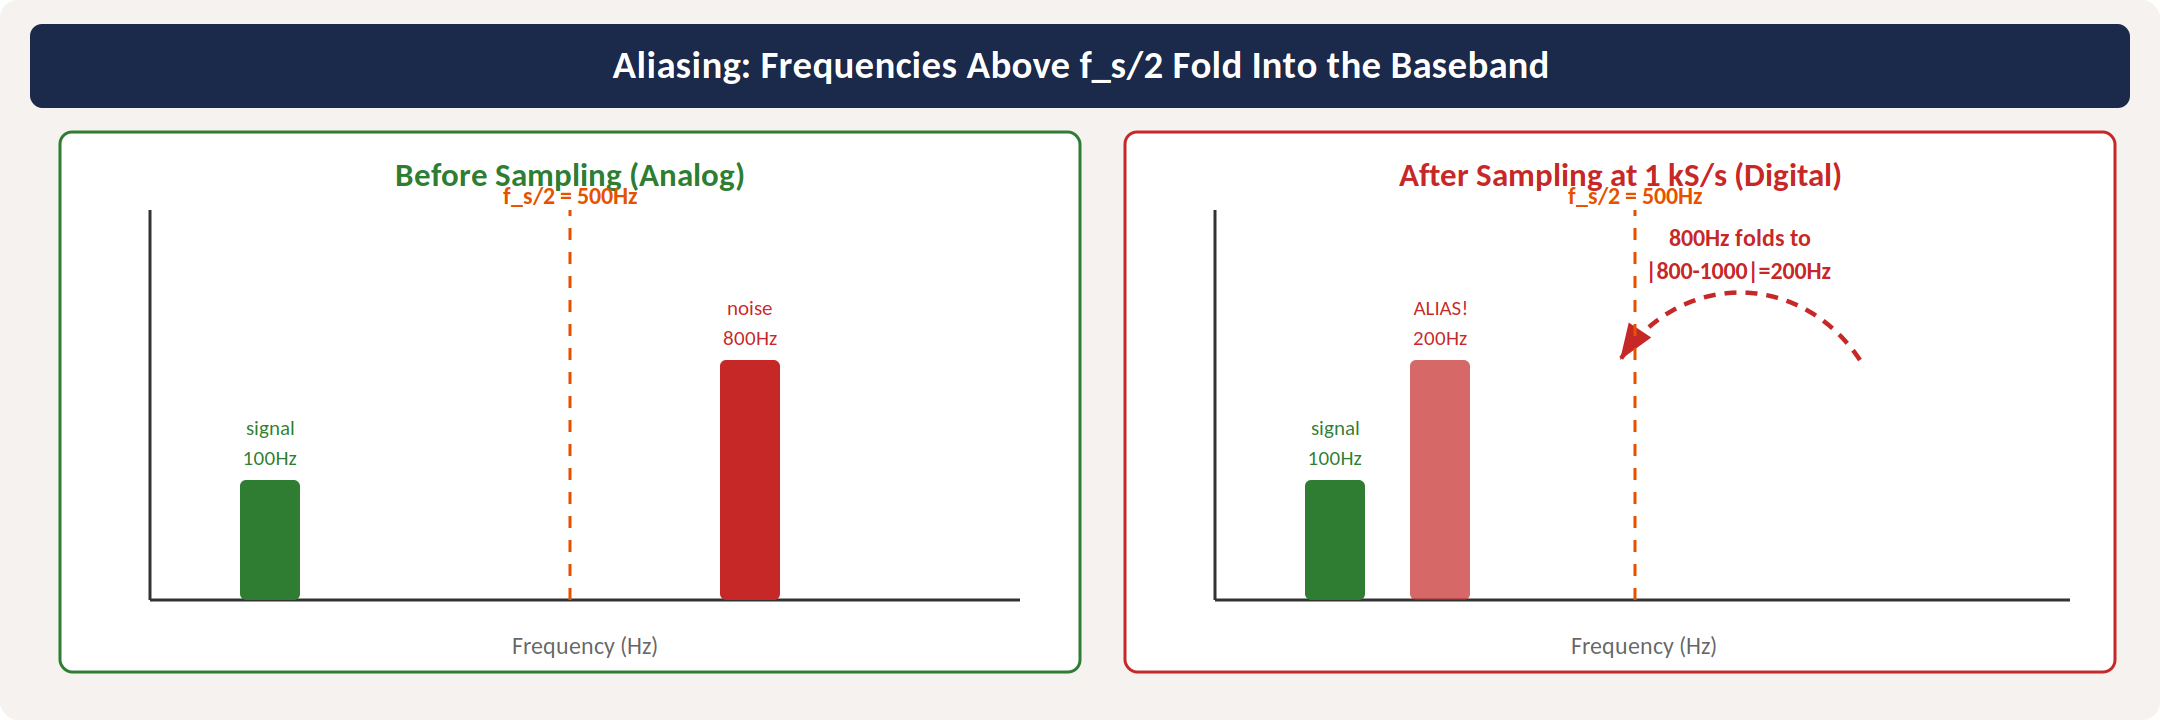
\includegraphics[width=\textwidth]{fig_aliasing.png}
\caption{Aliasing: an 800\,Hz noise component, sampled at 1\,kS/s, folds to 200\,Hz in the digital data. The alias is indistinguishable from a real 200\,Hz signal. Anti-alias filtering before the ADC is the only defense.}
\label{fig:aliasing}
\end{figure}

\begin{examplebox}[ThermoRig: Aliasing from a Switching Regulator]
The ThermoRig uses a 500\,kHz switching regulator that injects noise at 500\,kHz onto the thermocouple signal. The DAQ samples at 1\,kS/s ($f_s/2 = 500$\,Hz). Without an anti-alias filter, the 500\,kHz noise aliases to $|500000 - 500 \times 1000| = 0$\,Hz; it appears as a DC offset. A 2nd-order anti-alias filter at 400\,Hz attenuates 500\,kHz by $> 100$\,dB, making the alias negligible.
\end{examplebox}

\section{Practical Sampling Rate Selection}
\begin{itemize}[leftmargin=1.5em]
\item \textbf{Minimum}: $f_s > 2 f_{\max}$ (Nyquist criterion).
\item \textbf{Practical}: $f_s \geq 5 f_{\max}$ to $10 f_{\max}$ for good waveform reconstruction.
\item \textbf{For FFT analysis}: $f_s \geq 2.56 f_{\max}$ is common (the ``2.56 rule'' gives 25\% guard band for anti-alias filter roll-off).
\end{itemize}

\section{Quantization and Effective Number of Bits (ENOB)}
Real ADCs have noise, nonlinearity, and other imperfections that reduce their effective resolution below the nominal bit count. The ENOB is:
\begin{equation}
\text{ENOB} = \frac{\text{SINAD}_{\text{dB}} - 1.76}{6.02}
\end{equation}
where SINAD is the signal-to-noise-and-distortion ratio. A nominally 16-bit ADC might have ENOB of 14 bits in practice.


\section{Oversampling and Decimation}
Oversampling means sampling at a rate much higher than Nyquist ($f_s \gg 2f_{\max}$). Benefits:

\begin{itemize}[leftmargin=1.5em]
\item \textbf{Relaxes anti-alias filter requirements}: the transition band between the signal and the Nyquist frequency is wider, so a gentle analog filter suffices.
\item \textbf{Improves effective resolution}: oversampling by a factor of $4^k$ and digitally filtering/decimating adds $k$ bits of effective resolution. Example: a 12-bit ADC oversampled $64\times$ and decimated gains 3 effective bits (acts like a 15-bit ADC).
\item \textbf{Spreads quantization noise}: the same noise power is distributed over a wider bandwidth; filtering removes the out-of-band portion.
\end{itemize}

Modern sigma-delta ($\Sigma\Delta$) ADCs (used in precision instruments and audio) achieve 24-bit resolution by oversampling at 256$\times$ or more and using noise shaping to push quantization noise to high frequencies where it is filtered out.

\section{Dithering}
Adding a small amount of random noise (dither) to the ADC input, with amplitude $\approx$0.5--1\,LSB, actually \emph{improves} the measurement by breaking up quantization artifacts. The dither noise averages out over multiple samples, but it linearizes the ADC response and allows sub-LSB signals to be recovered through averaging. This is counterintuitive but mathematically sound and widely used in precision measurement.


\section{The Sampling Process in Detail}
When sampled at $f_s$, the signal spectrum is replicated at multiples of $f_s$. If content exists above $f_s/2$, replicas overlap the baseband, creating aliases.

\subsection{Alias Frequency Formula}
$f_{\text{alias}} = |f_{\text{signal}} - n \cdot f_s|$ where $n$ minimizes the result. Example: 900\,Hz at 1\,kS/s aliases to $|900-1000| = 100$\,Hz. Indistinguishable from a real 100\,Hz signal.

\section{Anti-Aliasing Strategy}
Step 1: determine signal bandwidth $f_{\max}$. Step 2: design analog LP filter with cutoff between $f_{\max}$ and $f_s/2$, sufficient rolloff to attenuate all content above $f_s/2$ below ADC noise floor. Step 3: set $f_s \geq 10 \times f_{\max}$.

\section{Oversampling Benefits}
Sampling much faster than Nyquist minimum: (1) relaxes anti-alias filter requirements; (2) spreads quantization noise over wider bandwidth, so digital filtering improves resolution ($\sim$0.5 bits per octave of oversampling); (3) improves time-domain resolution.

Sigma-delta ADCs exploit 64--256$\times$ oversampling with noise shaping to achieve 24-bit resolution at modest bandwidth.

\section{Dithering}
Adding small random noise before quantization linearizes the process when signal amplitude is comparable to LSB. The dither noise is then reduced by averaging, revealing sub-LSB signals.

\section{Reconstruction}
Converting digital to analog requires a DAC followed by a reconstruction filter (LP filter smoothing the staircase output). The ideal filter is a sinc function (brick-wall at $f_s/2$). In practice, smooth analog filters with zero-order hold compensation are used.

\section{Digital Resampling}
\textbf{Decimation}: reduce rate by factor $M$ (keep every $M$th sample after digital LP filter at $f_s/(2M)$). \textbf{Interpolation}: increase rate by factor $L$ (insert zeros, LP filter). Used for matching rates between instruments and reducing data size.

\begin{tipbox}[Common Aliasing Mistake]
Students set sampling rate based on signal frequency alone, forgetting about noise. If the signal is at 10\,Hz but the sensor picks up 60\,Hz and 500\,kHz noise, both will alias unless filtered before the ADC. The anti-alias filter must remove everything above $f_s/2$, not just above $f_{\max}$.
\end{tipbox}


\section{Practical Oversampling Design}
In many MEGN 300 labs, the DAQ is capable of much higher sample rates than needed. This excess capacity should be exploited. For a temperature signal with $f_{\max} = 1$\,Hz, instead of sampling at the minimum 10\,S/s, sample at 1000\,S/s. Then apply a digital low-pass filter at 5\,Hz and decimate by 100 to produce clean 10\,S/s data. Benefits: (1) the anti-alias filter only needs to attenuate at 500\,Hz (very easy), (2) quantization noise spread over 1000\,Hz band is reduced to the 5\,Hz signal band (23\,dB improvement, $\approx$4 extra bits of effective resolution), (3) the 60\,Hz noise and its harmonics are captured and can be digitally notch-filtered.

\section{Sample Rate for Control Systems}
In feedback control (Part IV), the controller must update fast enough that the digital sampling delay does not significantly degrade stability. The rule of thumb: $f_s \geq 20 \times f_{\text{crossover}}$ where $f_{\text{crossover}}$ is the loop bandwidth. For the ThermoRig with 0.2\,Hz bandwidth: $f_s \geq 4$\,Hz. We use 10\,Hz ($T_s = 100$\,ms) for comfortable margin. For a motor speed controller with 100\,Hz bandwidth: $f_s \geq 2$\,kHz.

\section{Data File Management}
Continuous acquisition at high sample rates generates large files. At 100\,kS/s with 16-bit resolution (2 bytes per sample): 200\,kB/s = 12\,MB/min = 720\,MB/hr. Plan storage accordingly. Use binary file formats (not text/CSV) for large datasets. LabVIEW's TDMS format provides efficient binary storage with metadata.
\section{The Z-Transform and Digital System Analysis}
Just as the Laplace transform ($s$-domain) is the analysis tool for continuous systems, the \textbf{z-transform} is the tool for discrete (sampled) systems. A discrete-time signal $x[n]$ has z-transform:
\begin{equation}
X(z) = \sum_{n=0}^{\infty} x[n] \, z^{-n}
\end{equation}
A digital filter's transfer function $H(z) = Y(z)/X(z)$ describes its frequency response when evaluated on the unit circle ($z = e^{j\omega T_s}$). Poles inside the unit circle ($|z| < 1$) produce stable, decaying responses; poles outside produce unstable, growing responses. This is the discrete-system equivalent of the left/right half-plane rule in the $s$-domain.

For MEGN~300, you do not need to design filters using the z-transform directly, but understanding that LabVIEW's digital filter VIs are implementing z-domain transfer functions helps you interpret their behavior and debug unexpected results.

\section{Quantization Effects in Digital Systems}
After sampling, the continuous-amplitude signal is quantized to $2^n$ discrete levels. This introduces two distinct effects:

\textbf{Quantization noise}: the difference between the true sample value and the nearest quantization level. For a properly dithered signal, this behaves as additive white noise with RMS value $\text{LSB}/\sqrt{12}$ and flat PSD up to $f_s/2$. The signal-to-quantization-noise ratio (SQNR) is $6.02n + 1.76$\,dB.

\textbf{Quantization distortion}: for small signals (amplitude comparable to a few LSBs), the quantization is no longer approximately linear. The ``staircase'' nature of the transfer function creates harmonic distortion. Dithering (adding noise of amplitude $\sim$1\,LSB before quantization) linearizes the process at the cost of a slightly higher noise floor.

\section{Practical Anti-Aliasing: A Complete Design Example}
Design an anti-aliasing system for measuring vibration from 0 to 500\,Hz:

\textbf{Step 1}: signal bandwidth $f_{\max} = 500$\,Hz. Choose $f_s = 2560$\,S/s (standard vibration analysis: $2.56 \times f_{\max}$, which gives 56\% oversampling above Nyquist minimum).

\textbf{Step 2}: Nyquist frequency $f_N = f_s/2 = 1280$\,Hz. The anti-alias filter must attenuate all content above 1280\,Hz below the ADC noise floor.

\textbf{Step 3}: for a 16-bit ADC (96\,dB dynamic range), require $\geq$96\,dB attenuation at $f_N$. A 4th-order Butterworth at $f_c = 640$\,Hz provides $-80$\,dB/decade rolloff. At $f_N = 1280$\,Hz ($= 2 \times f_c$): attenuation $= 4 \times 20\log_{10}(1280/640) = 4 \times 6 = 24$\,dB. Insufficient.

\textbf{Step 4}: increase to 8th-order (two cascaded 4th-order stages): $-160$\,dB/decade. At $f_N$: $8 \times 6 = 48$\,dB. Still insufficient for 16-bit, but adequate for 8-bit. For 16-bit, either increase the sample rate (more oversampling) or use a higher-order filter.

\textbf{Step 5}: alternatively, oversample at $f_s = 10{,}240$\,S/s ($20\times f_{\max}$). Now $f_N = 5120$\,Hz. A 4th-order Butterworth at $f_c = 640$\,Hz provides $-80\log_{10}(5120/640) = -80 \times 0.903 = 72$\,dB at $f_N$. Combined with subsequent digital filtering and decimation: adequate for 14-bit.

This example illustrates the fundamental tradeoff: sharper anti-alias filters allow lower sample rates, while higher sample rates allow simpler anti-alias filters.

\section{Multirate Signal Processing}
Many practical systems use multirate processing: acquire at a high sample rate (to simplify anti-aliasing), then decimate digitally to the rate needed for analysis or control.

\textbf{Decimation by M}: (1) apply a digital LP filter with cutoff at $f_s/(2M)$ to prevent aliasing; (2) discard $M-1$ out of every $M$ samples. The output rate is $f_s/M$. Example: acquire at 10\,kS/s, decimate by 10 to 1\,kS/s. The digital anti-alias filter at 500\,Hz can be very sharp (100th-order FIR) because computation is cheap.

\textbf{Multistage decimation}: for large decimation ratios, cascade multiple smaller stages. Decimating by 100 as $10 \times 10$ requires fewer total filter taps than a single $100\times$ decimation. Each stage's filter only needs to handle its own Nyquist constraint.

\section{Sigma-Delta Conversion in Detail}
The sigma-delta ADC deserves deeper treatment because it is the dominant technology for precision measurement.

The sigma-delta modulator oversamples the input at rate $K \times f_s$ (where $K = 64$--$256$ is the oversampling ratio and $f_s$ is the output rate). A 1-bit quantizer in a feedback loop with an integrator ``shapes'' the quantization noise, pushing most of it to high frequencies. A subsequent digital decimation filter (sinc$^3$ or sinc$^4$) removes this high-frequency noise and reduces the data rate to $f_s$.

The result: from a simple 1-bit converter, you achieve 24-bit resolution in the output band. The tradeoff is latency: the decimation filter introduces a delay of several hundred output sample periods. For the ThermoRig at 10\,S/s output rate: latency $\approx 0.3$\,s. This is acceptable for temperature measurement but would be too slow for a fast control loop.
\section{Complete Anti-Aliasing Design: A Worked Example}
Design a measurement system for capturing vibration signatures of a small DC motor (0--1\,kHz bandwidth) using an NI USB-6001 (14-bit, max 20\,kS/s).

\textbf{Step 1: Sample rate.} For $f_{\max} = 1$\,kHz: $f_s = 2.56 \times 1000 = 2560$\,S/s minimum. Choose $f_s = 5120$\,S/s (power of 2 $\times$ 10, convenient for FFT with $N = 5120$). Nyquist: $f_N = 2560$\,Hz.

\textbf{Step 2: Anti-alias filter.} Need $\geq 6.02 \times 14 = 84$\,dB attenuation at $f_N = 2560$\,Hz. Choose $f_c = 1280$\,Hz (octave above $f_{\max}$). Required order $n$ for Butterworth: $n \geq 84/(20\log_{10}(2560/1280)) = 84/6.02 = 14$. An 8th-order Butterworth (four cascaded Sallen-Key stages) provides $8 \times 6 = 48$\,dB at $f_N$, insufficient.

\textbf{Step 3: Increase oversampling.} Instead, sample at $f_s = 20{,}480$\,S/s ($20\times f_{\max}$). Now $f_N = 10{,}240$\,Hz. A 4th-order Butterworth at $f_c = 1280$\,Hz provides $4 \times 20\log_{10}(10240/1280) = 4 \times 18.1 = 72$\,dB at $f_N$. Marginally adequate for 14-bit. Add a 6th-order ($3\times$ Sallen-Key) for 108\,dB: comfortable margin.

\textbf{Step 4: Digital decimation.} After acquisition at 20\,kS/s, apply a digital LP at 1280\,Hz (sharp FIR, 200 taps) and decimate by 4 to 5\,kS/s output. This gives 1\,Hz frequency resolution with $N = 5000$ points.

This example illustrates the oversampling + digital decimation strategy that is standard in modern instrumentation: use a high sample rate to simplify the analog anti-alias filter, then do the sharp filtering digitally where precision is free.
\section{Choosing the Right Sample Rate: A Decision Framework}
The sample rate $f_s$ is one of the most important design decisions in a measurement system. Too low: aliasing corrupts data. Too high: generates excessive data volume, increases computational load, and may exceed DAQ bandwidth when using many channels. The right choice depends on the application:

\textbf{DC and slowly varying measurements} (temperature, static pressure, weight): $f_s = 10$--$100$\,S/s. The signal bandwidth is $< 1$\,Hz, so even $10\times$ oversampling requires only 10\,S/s. Higher rates are useful only for oversampling-based resolution enhancement.

\textbf{Low-frequency dynamic measurements} (building vibration, ocean waves, biological signals): $f_s = 100$--$1000$\,S/s. Signal bandwidth up to 50\,Hz.

\textbf{General vibration and acoustics}: $f_s = 2{,}560$--$51{,}200$\,S/s. Signal bandwidth 100\,Hz to 20\,kHz. The standard vibration analysis rate is $2.56 \times f_{\max}$ (providing adequate oversampling for Hanning-windowed FFT).

\textbf{High-speed transients} (impact, shock, ultrasonic): $f_s = 100$\,kS/s to 100\,MS/s. Signal bandwidth 10\,kHz to 50\,MHz. Requires high-speed DAQ hardware (oscilloscopes or dedicated high-speed digitizers).

\section{Data Volume and Storage Calculations}
At $f_s = 100$\,kS/s with 16-bit resolution: data rate $= 200$\,kB/s $= 12$\,MB/min $= 720$\,MB/hr. For a 24-hour monitoring session: 17.3\,GB. For 8 channels simultaneously: 138\,GB. Plan storage and file format accordingly:

\textbf{Binary formats} (TDMS, HDF5, raw binary): compact, fast to write, preserves full precision. TDMS (NI's Technical Data Management Streaming) is native to LabVIEW and includes metadata headers.

\textbf{Text formats} (CSV, tab-delimited): human-readable but 3--10$\times$ larger than binary (each 16-bit sample uses 2 bytes in binary but 5--6 characters in text). Writing speed is also slower due to number-to-text conversion. Use for small datasets or interoperability with Excel.

\textbf{Compression}: lossless compression (ZIP, gzip) typically reduces measurement data by 30--50\%. Lossy compression (reducing precision from 16-bit to 12-bit) saves 25\% but discards information permanently.

\section{Discrete Convolution}
Convolution is the fundamental operation of digital filtering. The output of an FIR filter is the discrete convolution of the input signal $x[n]$ with the filter's impulse response $h[n]$:
\begin{equation}
y[n] = \sum_{k=0}^{M-1} h[k] \cdot x[n-k] = (x * h)[n]
\end{equation}
In the frequency domain, convolution becomes multiplication: $Y(f) = X(f) \cdot H(f)$. This duality is the foundation of all frequency-domain signal processing: multiplying the signal spectrum by the filter's frequency response is equivalent to convolving the signal with the filter's impulse response in the time domain.

LabVIEW implements convolution via the ``Convolution'' VI in the Signal Processing palette, or implicitly when you use any filter VI (which convolves the input with the filter coefficients).

\section{The Sampling Theorem: Proof by Intuition}
Why must $f_s > 2f_{\max}$? Consider a sine wave at frequency $f$. To uniquely identify this sine wave, you need to determine three parameters: frequency, amplitude, and phase. Each parameter requires at least one constraint, and each sample provides one constraint. Therefore, you need at least two samples per cycle ($f_s > 2f$) to determine a single sinusoid. With fewer than two samples per cycle, you cannot distinguish the sinusoid from a lower-frequency alias.

At exactly $f_s = 2f$ (sampling at the Nyquist rate): the samples fall at the same phase of each cycle. If they fall at the zero crossings, the measured amplitude is zero regardless of the true amplitude. This is why the inequality is strict: $f_s > 2f_{\max}$, not $f_s \geq 2f_{\max}$.

\section{Practical Aliasing Scenarios in MEGN 300}
\textbf{Scenario 1: Switching noise.} A DC-DC converter on the power supply board operates at 500\,kHz. The thermocouple wiring picks up 5\,mV of this noise. Sampled at 1\,kS/s: the 500\,kHz noise aliases to $|500{,}000 - 500 \times 1000| = 0$\,Hz (DC), appearing as a constant offset. Worse: it aliases to DC \emph{only when the switching frequency is an exact multiple of the sample rate}. If the switching frequency drifts slightly (to 500.1\,kHz): the alias appears at 100\,Hz, creating an unexplained oscillation in the data.

\textbf{Scenario 2: Motor commutation.} A brushed DC motor commutates at $N_{\text{segments}} \times f_{\text{rotation}}$. For a 3-segment commutator at 10{,}000\,RPM: $f_{\text{comm}} = 3 \times 166.7 = 500$\,Hz. If the vibration sensor is sampled at 800\,S/s: the 500\,Hz vibration aliases to $|500 - 800| = 300$\,Hz, appearing as a false vibration that does not correspond to any physical phenomenon.

\textbf{Scenario 3: Fluorescent lighting.} Fluorescent lights flicker at twice the mains frequency (120\,Hz in the US). A photodiode measuring ambient light sampled at 100\,S/s: the 120\,Hz flicker aliases to $|120 - 100| = 20$\,Hz, appearing as a slow oscillation in the light level.

In all three scenarios, the solution is the same: an analog anti-alias filter before the ADC, with cutoff below $f_s/2$.
\section{Digital Filtering in LabVIEW: Implementation Patterns}
Three common implementation patterns for digital filtering in LabVIEW real-time applications:

\textbf{Pattern 1: Block processing.} Acquire a block of $N$ samples, apply the filter to the entire block, process the result. Simple but introduces latency of $N/f_s$ seconds. Suitable for offline analysis and non-real-time monitoring.

\textbf{Pattern 2: Sample-by-sample with shift registers.} In a While Loop, read one sample per iteration. Use shift registers to store the filter state (past inputs and outputs). Apply the filter equation to produce one output sample. This provides minimum latency (one sample period) and is the pattern for real-time control loops. The shift register count equals the filter order.

\textbf{Pattern 3: Streaming with overlap.} Acquire blocks of $N$ samples with overlap. Apply the filter to each block, then stitch the results using overlap-add or overlap-save. This is the most efficient for long FIR filters because it uses FFT-based convolution (which is $O(N\log N)$ instead of $O(NM)$ for direct convolution). LabVIEW's ``Convolution'' VI uses this approach internally.

\section{Resampling: Practical Considerations}
When combining data from two sources sampled at different rates (e.g., a vibration signal at 10\,kS/s and a tachometer at 1\,kS/s), resampling aligns the time bases:

\textbf{Upsampling} (interpolation): insert zeros between samples, then low-pass filter to smooth. In LabVIEW: the ``Resample Waveforms'' VI. Quality depends on the interpolation filter; use cubic or sinc interpolation for measurement-quality results. Linear interpolation introduces high-frequency distortion.

\textbf{Downsampling} (decimation): low-pass filter to prevent aliasing, then discard samples. The anti-alias filter cutoff must be at the new Nyquist frequency ($f_{s,\text{new}}/2$), not the original.

\textbf{Rational resampling}: for non-integer rate ratios (e.g., converting from 44.1\,kS/s to 48\,kS/s, ratio $= 160/147$): first upsample by 160, then downsample by 147 (or use a polyphase filter that combines both operations efficiently).

\section{Spectral Analysis of Noise}
The noise floor of a measurement system is best characterized by its Power Spectral Density (PSD). To measure the system PSD:

(1) Short the input (zero signal). (2) Acquire a long record ($T \geq 10$\,s for thermal noise characterization). (3) Compute the PSD using Welch's method (averaged, overlapped FFTs). (4) Plot in units of V$^2$/Hz or V/$\sqrt{\text{Hz}}$ vs.\ frequency.

The PSD reveals the noise character: \textbf{white noise} (flat PSD) indicates thermal noise or quantization noise dominating. \textbf{1/f noise} (PSD rising at low frequencies) indicates flicker noise in semiconductors. \textbf{Discrete peaks} indicate EMI at specific frequencies.

The total RMS noise in a measurement with bandwidth $B$ is:
\begin{equation}
V_{n,\text{RMS}} = \sqrt{\int_0^B \text{PSD}(f)\,df}
\end{equation}
For white noise with PSD $= S_0$: $V_{n,\text{RMS}} = \sqrt{S_0 \cdot B}$. Halving $B$ reduces noise by $\sqrt{2}$ (3\,dB).
\section{The Z-Transform: Bridge from Continuous to Digital}
The Laplace transform ($s$-domain) describes continuous-time systems. The \textbf{z-transform} is its discrete-time counterpart. Understanding the $s$-to-$z$ mapping is essential for analyzing digital control loops (Chapter~16) and digital filters (Chapter~12).

\subsection{Definition}
For a discrete-time signal $x[n]$: $X(z) = \sum_{n=0}^{\infty} x[n] z^{-n}$. The variable $z = e^{sT_s}$ relates the $z$-domain to the $s$-domain, where $T_s = 1/f_s$ is the sample period.

\subsection{Key Mapping: Poles and Stability}
In the $s$-domain, stability requires all poles in the left half-plane ($\text{Re}(s) < 0$). The mapping $z = e^{sT_s}$ transforms the left half-plane into the interior of the unit circle ($|z| < 1$). Therefore, in the $z$-domain, stability requires all poles inside the unit circle.

The imaginary axis ($\text{Re}(s) = 0$) maps to the unit circle ($|z| = 1$). Frequencies map as: $\omega = 0$ (DC) maps to $z = 1$. The Nyquist frequency $\omega = \pi/T_s$ maps to $z = -1$. Frequencies between 0 and Nyquist trace the upper half of the unit circle.

\subsection{Bilinear Transform}
The most common method for converting an analog filter or controller design to digital form: $s = \frac{2}{T_s} \frac{1 - z^{-1}}{1 + z^{-1}}$. This maps the entire left half-plane to the interior of the unit circle (preserving stability) with a nonlinear frequency warping: $\omega_{\text{digital}} = (2/T_s)\tan(\omega_{\text{analog}} T_s/2)$. The warping is negligible for $\omega_{\text{analog}} \ll \pi/T_s$ but becomes significant near Nyquist. Pre-warp the analog cutoff frequency before applying the bilinear transform to ensure the digital filter has the correct cutoff.

\subsection{Why This Matters for Control}
A PI controller designed in the $s$-domain as $G_c(s) = K_p + K_i/s$ must be converted to the $z$-domain for digital implementation. The simplest method (backward Euler): $1/s \to T_s/(1 - z^{-1})$, giving $G_c(z) = K_p + K_i T_s / (1 - z^{-1})$. This is exactly the discrete PID summation used in Chapter~16. The bilinear transform gives a slightly different (and more accurate) discretization: $1/s \to (T_s/2)(1 + z^{-1})/(1 - z^{-1})$, called the Tustin method. For slow loops ($f_s \gg 10 \times f_{\text{bandwidth}}$), the methods are equivalent. For fast loops ($f_s < 20 \times f_{\text{bandwidth}}$), the Tustin method better preserves the analog design's stability margins.

\begin{tipbox}[When to Worry About the $s$-to-$z$ Mapping]
For MEGN~300 thermal control systems ($f_{\text{bandwidth}} < 0.1$\,Hz, $f_s \geq 10$\,Hz): the ratio $f_s/f_{\text{bandwidth}} > 100$. At this ratio, all discretization methods (Euler, Tustin, exact ZOH) give identical results. The $s$-to-$z$ mapping becomes important when this ratio drops below 20, which occurs in fast mechanical and electrical control systems but not in typical instrumentation lab projects.
\end{tipbox}
\section{Practice Questions}
\begin{enumerate}[leftmargin=1.5em]
\item A 500\,Hz signal is sampled at 800\,S/s. What frequency appears in the digital data? Is this the true signal or an alias?
\item Design an anti-aliasing filter for a DAQ system sampling at 10\,kS/s. The signal of interest spans 0--2\,kHz. Specify the filter type, cutoff frequency, and minimum order if the filter must attenuate frequencies above 5\,kHz by at least 40\,dB.
\item A 12-bit ADC with a 10\,V range has a measured SINAD of 68\,dB. Calculate the ENOB. How many bits of resolution are ``lost'' to noise and distortion?
\end{enumerate}

\subsection{Answers}
\begin{enumerate}[leftmargin=1.5em]
\item $f_s/2 = 400$\,Hz. Since 500 $>$ 400, it aliases. $f_{\text{alias}} = |500 - 1 \times 800| = 300$\,Hz. A false 300\,Hz signal appears in the data; the true 500\,Hz signal is lost.
\item Anti-alias cutoff: set at 4\,kHz (to pass the 0--2\,kHz signal band with margin and begin rolling off before Nyquist at 5\,kHz). For 40\,dB attenuation in the range 5--10\,kHz: a 4th-order Butterworth ($-80$\,dB/decade) provides 40\,dB attenuation at 1.25 decades above cutoff... actually at 5\,kHz ($5/4 = 1.25\times$ cutoff): attenuation $= 20 \times 4 \times \log_{10}(1.25) = 7.7$\,dB (not enough). A better approach: set cutoff at 3\,kHz. At 5\,kHz: $5/3 = 1.67\times$, 4th-order attenuation $= 80 \times \log_{10}(1.67) = 17.8$\,dB (still not enough for $-40$\,dB). Need higher order or lower cutoff. An 8th-order Butterworth at 3.5\,kHz gives $-160 \times \log_{10}(5/3.5) = -24.8$\,dB at 5\,kHz; still short. Practical solution: use a 4th-order Butterworth at 2.5\,kHz, which gives $-80 \times \log_{10}(5/2.5) = -24$\,dB at 5\,kHz. With oversampling (sample at 50\,kS/s, digitally filter, then decimate to 10\,kS/s), the analog filter requirements relax dramatically. This is the standard approach in modern DAQ systems.
\item ENOB $= (68 - 1.76)/6.02 = 11.0$ bits. The ADC loses 1.0 bit of effective resolution to noise and distortion.
\end{enumerate}


% ================================================================
\chapter{Analog Filter Design}

\section{What Filters Do}
A filter selectively passes or rejects frequency components of a signal. Four basic types:
\begin{itemize}[nosep,leftmargin=1.5em]
\item \textbf{Low-pass}: passes frequencies below cutoff $f_c$; attenuates above. The most common in instrumentation (anti-aliasing, noise reduction).
\item \textbf{High-pass}: passes frequencies above $f_c$; attenuates below. Removes DC offset and low-frequency drift.
\item \textbf{Band-pass}: passes a band between $f_L$ and $f_H$; attenuates outside. Isolates a signal of interest.
\item \textbf{Band-stop (notch)}: rejects a narrow band around a center frequency. Removes a specific interference (e.g., 60\,Hz hum).
\end{itemize}

\begin{figure}[htbp]
\centering
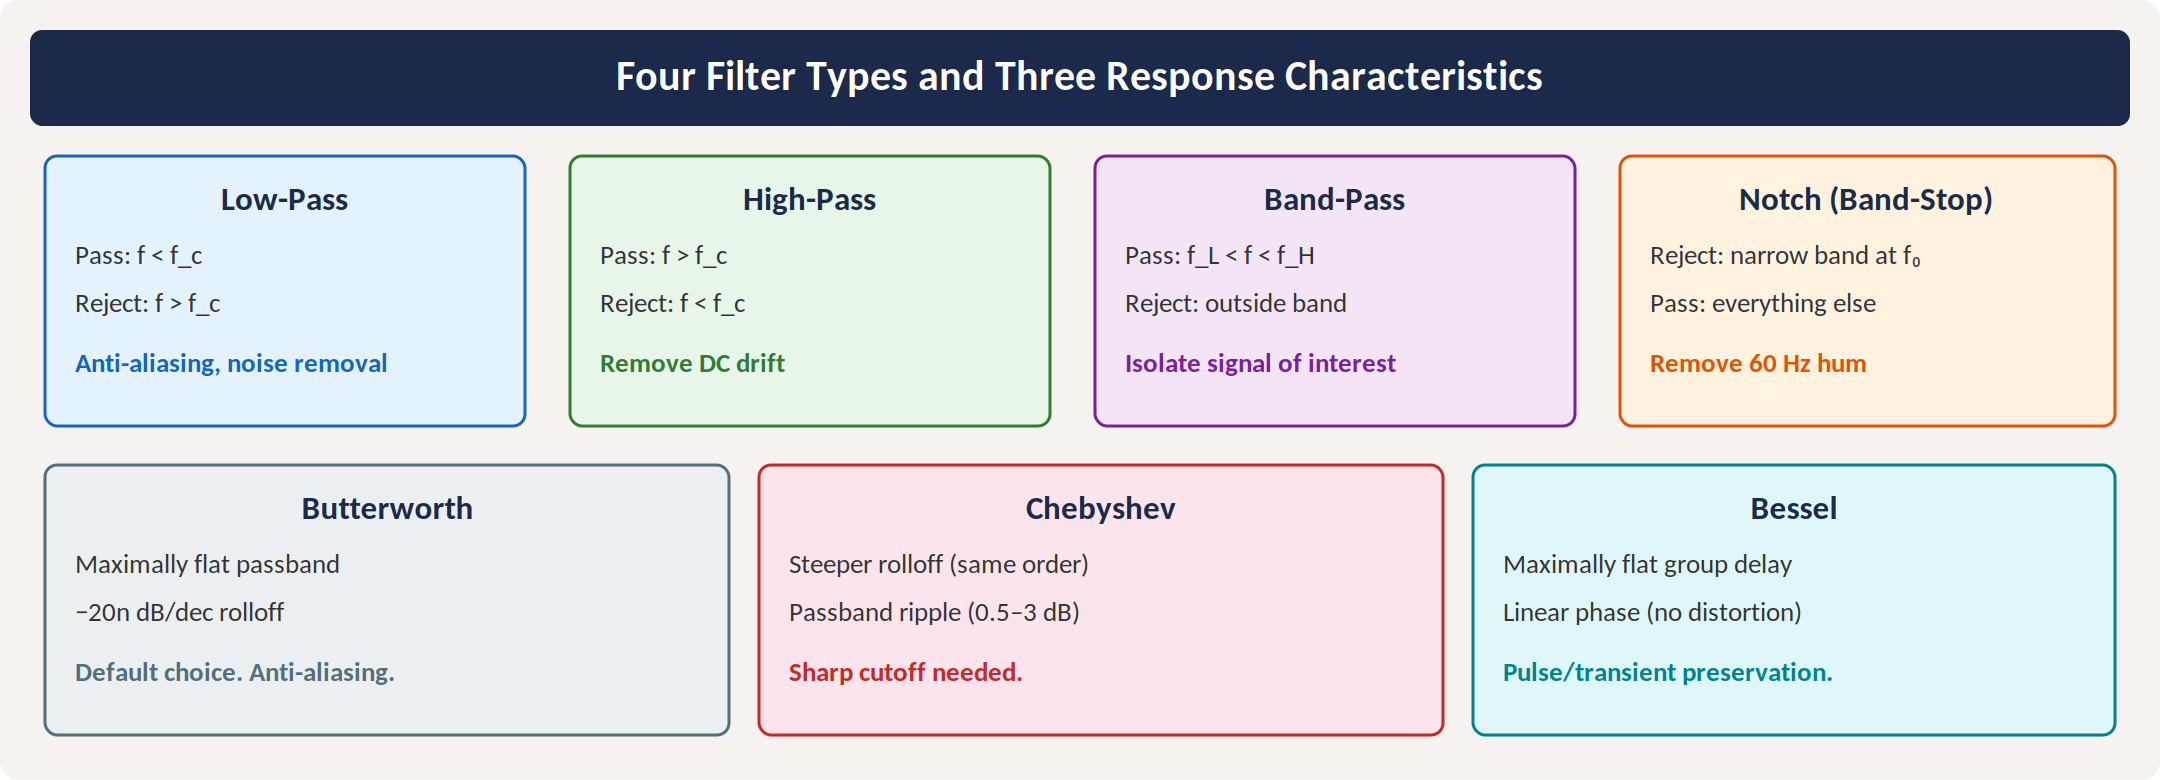
\includegraphics[width=\textwidth]{fig_filter_types.png}
\caption{Four filter types (top) and three response characteristics (bottom). Butterworth is the default; Chebyshev for sharp cutoff; Bessel for pulse preservation.}
\label{fig:filters}
\end{figure}

\section{Passive RC Filters}
The simplest filter: one resistor and one capacitor.

\subsection{First-Order Low-Pass}
RC in series; output across the capacitor.
\begin{equation}
f_c = \frac{1}{2\pi RC}, \qquad H(j\omega) = \frac{1}{1 + j\omega RC}
\end{equation}
Magnitude rolls off at $-20$\,dB/decade above $f_c$. Phase shifts from 0\ang{} (DC) to $-90$\ang{} (high frequency), passing through $-45$\ang{} at $f_c$.

\subsection{First-Order High-Pass}
Same components; output across the resistor.
\begin{equation}
f_c = \frac{1}{2\pi RC}, \qquad H(j\omega) = \frac{j\omega RC}{1 + j\omega RC}
\end{equation}
Passes frequencies above $f_c$; $-20$\,dB/decade roll-off below $f_c$.

\section{Active Filters}
Active filters use operational amplifiers to provide gain, buffering, and steeper roll-off without the signal attenuation inherent in passive filters. The Sallen-Key topology is the most common for second-order sections.

\subsection{Filter Response Types}
\textbf{Butterworth}: maximally flat magnitude in the passband. No ripple. The standard choice when flat amplitude response is more important than sharp cutoff. Roll-off: $-20n$\,dB/decade for $n$-th order.

\textbf{Chebyshev Type I}: steeper roll-off than Butterworth for the same order, but introduces ripple in the passband. Use when sharp cutoff is more important than flat passband.

\textbf{Bessel}: maximally flat group delay (linear phase). The best choice for time-domain measurements (pulse shapes, step responses) where phase distortion must be minimized.

\begin{figure}[htbp]
\centering
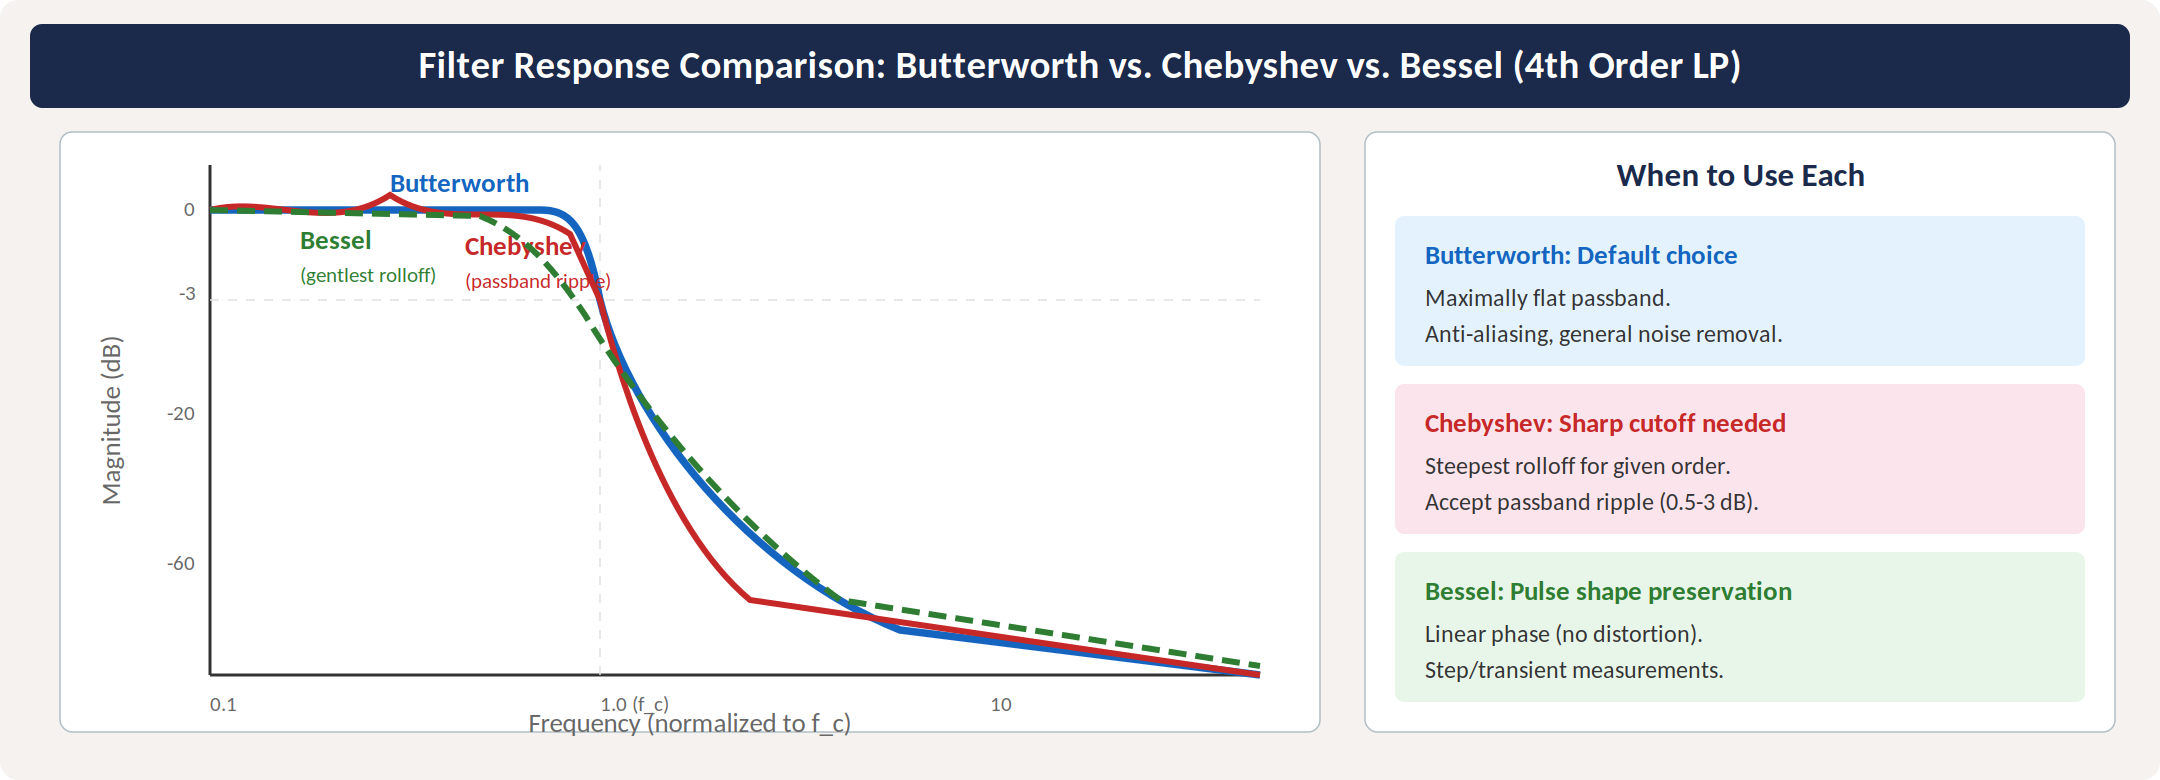
\includegraphics[width=\textwidth]{fig_filter_comparison.png}
\caption{Bode magnitude comparison of 4th-order Butterworth, Chebyshev, and Bessel low-pass filters. Chebyshev has the steepest rolloff but introduces passband ripple. Bessel has the gentlest rolloff but preserves pulse shape (linear phase).}
\label{fig:filter_compare}
\end{figure}

\begin{tipbox}[Choosing a Filter Type]
For anti-aliasing: Butterworth (flat passband). For isolating a specific frequency: Chebyshev (sharp cutoff). For preserving pulse shape: Bessel (linear phase). When in doubt, use Butterworth.
\end{tipbox}


\section{Designing Active Filters with Op-Amps}

\subsection{Sallen-Key Low-Pass (Second-Order)}
The Sallen-Key topology uses a single op-amp in a non-inverting configuration with positive feedback through capacitors. For a unity-gain second-order Butterworth low-pass:
\begin{equation}
f_c = \frac{1}{2\pi\sqrt{R_1 R_2 C_1 C_2}}
\end{equation}
For Butterworth response (maximally flat), set $C_2 = 2C_1$ and $R_1 = R_2 = R$:
\begin{equation}
f_c = \frac{1}{2\pi R \sqrt{2C_1^2}} = \frac{1}{2\pi R C_1 \sqrt{2}}
\end{equation}

\textbf{Design procedure} for a 2nd-order Butterworth LP at $f_c$:
\begin{enumerate}[nosep,leftmargin=1.5em]
\item Choose $C_1$ (typically 1--100\,nF for audio/instrumentation frequencies).
\item Set $C_2 = 2 C_1$.
\item Calculate $R = R_1 = R_2 = 1/(2\pi f_c C_1 \sqrt{2})$.
\item Select the nearest standard resistor value.
\item Use a unity-gain stable op-amp (e.g., TL072, OPA2134, or MCP6002 for 3.3\,V systems).
\end{enumerate}

\subsection{Higher-Order Filters}
Higher-order filters are built by cascading second-order sections. A 4th-order Butterworth = two cascaded 2nd-order Sallen-Key stages, each with a specific $Q$ value (1st stage: $Q = 0.541$; 2nd stage: $Q = 1.307$). Filter design tables (or software like FilterPro, Analog Devices Filter Wizard) provide the component values for each stage.

\begin{tipbox}[Use Filter Design Software]
Do not calculate high-order filter components by hand. Use Texas Instruments FilterPro, Analog Devices Filter Wizard, or the MathWorks Filter Designer. Input your requirements (type, order, cutoff, passband ripple) and the tool outputs a complete schematic with component values. Verify in SPICE simulation before building.
\end{tipbox}


\section{Why Analog Filters Are Essential}
Digital filters (Chapter 11) operate on digitized signals only. Before the ADC, the only noise removal tool is an analog filter. The anti-alias filter (analog LP before ADC) is mandatory; without it, aliasing permanently corrupts digital data.

\section{First-Order RC Low-Pass Filter}
$f_c = 1/(2\pi RC)$. At $f_c$: $-3$\,dB. Above: $-20$\,dB/decade. Rarely adequate for anti-aliasing; at $10\times f_c$, only $-20$\,dB attenuation passes through. Choose $R$ in 1--100\,k$\Omega$ range (balance current draw vs.\ thermal noise).

\section{Sallen-Key Active Filters}
Second-order ($-40$\,dB/decade) with one op-amp. Equal-component design ($R_1 = R_2$, $C_1 = C_2$): $f_c = 1/(2\pi RC)$. For Butterworth response ($Q = 0.707$), set gain $G = 1.586$. Cascade two stages for 4th order ($-80$\,dB/decade).

\section{Filter Types}
\textbf{Butterworth}: maximally flat passband. No ripple. Default for general-purpose and anti-aliasing. $|H(f)| = 1/\sqrt{1+(f/f_c)^{2n}}$.

\textbf{Chebyshev Type I}: steepest rolloff for given order. Accepts 0.5--3\,dB passband ripple. Use when maximum rejection of a nearby interferer is needed.

\textbf{Bessel}: most linear phase (constant group delay). Preserves pulse shape. Gentlest rolloff. Use for time-domain transient measurements.

\begin{warningbox}[Phase Delay and Control Stability]
Higher-order filters introduce more phase lag. A 4th-order Butterworth at 100\,Hz has $\sim$180$^\circ$ lag at cutoff. In control loops, this reduces phase margin and can cause instability. Limit filter order and set cutoff well above control bandwidth.
\end{warningbox}

\section{Notch Filters}
A notch (band-reject) filter removes a specific frequency (e.g., 60\,Hz) while passing all others. Twin-T passive topology achieves $-40$ to $-60$\,dB rejection. However, if interference has harmonics, each needs its own notch. Fixing grounding and shielding is often a better solution.

\section{Design Workflow}
(1) Determine $f_{\max}$ and $f_s$. (2) Set $f_c$ between $f_{\max}$ and $f_s/2$ (common: $f_c = f_s/4$). (3) Required stopband attenuation at $f_s/2$: $\geq 6n$\,dB for $n$-bit ADC. (4) Choose filter type. (5) Calculate order: $n \geq \text{attenuation}/(20\log_{10}(f_s/(2f_c)))$ for Butterworth. (6) Implement with cascaded Sallen-Key stages. (7) Measure actual response.


\section{Component Selection for Filters}
Real components have parasitic properties that affect filter performance. Resistors have parasitic inductance (wire-wound types: 1--10\,$\mu$H) and capacitance (0.1--1\,pF). Carbon film and thin-film resistors are preferred for filter applications. Capacitors have parasitic ESR (equivalent series resistance) and ESL (inductance). Ceramic (C0G/NP0) are best for filter applications: low ESR, low temperature coefficient, stable capacitance. Avoid Y5V and Z5U ceramics (capacitance varies 20--80\% with temperature and voltage).

\section{Active Filter Power Supply Considerations}
The op-amp in a Sallen-Key filter needs headroom above and below the signal swing. For a 0--5\,V signal, use $\pm$12\,V or $\pm$15\,V bipolar supply (or a single 12\,V supply with mid-rail virtual ground). Single-supply op-amps (rail-to-rail input/output) can operate on 5\,V, but the signal must be biased to mid-supply for maximum dynamic range.

\section{Measuring Filter Response}
After building a filter, verify its frequency response experimentally: (1) Apply a sine wave from a function generator. (2) Sweep the frequency from $0.1 f_c$ to $10 f_c$ in 10--20 steps. (3) At each frequency, measure the input and output amplitudes (RMS voltmeters or oscilloscope). (4) Compute the gain $G = V_{\text{out}}/V_{\text{in}}$ and convert to dB. (5) Plot the Bode magnitude diagram and verify it matches the design. Deviations indicate component tolerances, parasitic effects, or wiring errors.

\section{Switched-Capacitor Filters}
An alternative to traditional RC active filters, switched-capacitor filters use a clock signal to simulate resistors with capacitor-switch networks. The ``resistance'' is $R_{\text{eq}} = 1/(f_{\text{clk}} C)$, so the cutoff frequency scales linearly with the clock frequency. This allows easy, precise frequency tuning by changing a single clock signal. Available as complete ICs (e.g., MAX291/MAX292 for 8th-order Butterworth). Ideal for applications needing multiple filter frequencies or temperature-insensitive cutoff.
\section{Active Filter Component Sensitivity}
Real components have tolerances (1\% for standard resistors, 5--10\% for ceramic capacitors). These tolerances shift the actual filter cutoff frequency and $Q$ from the design values.

For a Sallen-Key filter with equal components ($R$, $C$): the cutoff frequency $f_c = 1/(2\pi RC)$ has a sensitivity of $-1$ to both $R$ and $C$: a 1\% increase in $R$ decreases $f_c$ by 1\%. With 1\% resistors and 5\% capacitors, the worst-case $f_c$ deviation is approximately $\pm$6\%. For anti-aliasing, this means designing with a safety margin: set $f_c$ at 80\% of the desired value to ensure the actual cutoff never exceeds the target.

For the $Q$ factor, sensitivity depends on the topology. In the Sallen-Key, $Q$ is sensitive to the gain-setting resistors. A 1\% mismatch can shift $Q$ by 5--10\%, potentially causing peaking or reduced rolloff in a Butterworth design. Solution: use 0.1\% resistors for the gain network, or use a topology less sensitive to $Q$ (Multiple Feedback or State Variable).

\section{Multiple Feedback (MFB) Topology}
The MFB is an alternative to Sallen-Key that provides an inverting output and has lower sensitivity to component variations for high-$Q$ designs. The transfer function:
\begin{equation}
H(s) = \frac{-1/(R_1 R_3 C_1 C_2)}{s^2 + s(1/R_1 + 1/R_3)/(C_2) + 1/(R_2 R_3 C_1 C_2)}
\end{equation}
The MFB is preferred when $Q > 2$ because the Sallen-Key requires gain close to 3, which makes it sensitive to gain-resistor tolerance. The MFB achieves high $Q$ without high gain, reducing sensitivity.

\section{State Variable Filter}
The state-variable (or biquad) topology uses two integrators and a summing amplifier to provide simultaneous low-pass, band-pass, and high-pass outputs from a single circuit. Advantages: $f_c$ and $Q$ can be adjusted independently (by changing different component values), and the circuit is less sensitive to component tolerances than Sallen-Key at high $Q$. Disadvantage: requires three op-amps per second-order section (vs.\ one for Sallen-Key).

The state variable is the topology of choice for tunable filters, notch filters (by summing the LP and HP outputs), and precision band-pass filters used in vibration analysis.

\section{Switched-Capacitor Filters}
Switched-capacitor (SC) filters simulate resistors using capacitors and electronic switches: $R_{\text{eq}} = 1/(f_{\text{clk}} \cdot C)$. By changing the clock frequency, the cutoff frequency changes proportionally. Available as complete ICs:

\textbf{MAX291/MAX292}: 8th-order Butterworth or Bessel LP. Clock-to-cutoff ratio of 100:1. For $f_c = 1$\,kHz: apply a 100\,kHz clock. For $f_c = 10$\,Hz: apply a 1\,kHz clock. No external components needed beyond a clock source and decoupling capacitors.

\textbf{LTC1068}: quad 2nd-order sections configurable as LP, HP, BP, or notch. For complex filter shapes.

SC filters are ideal for anti-aliasing in systems where the sample rate (and therefore the required $f_c$) changes dynamically. They introduce clock feedthrough noise at $f_{\text{clk}}$ and its harmonics, which must be removed by a simple RC post-filter.

\section{Filter Design Software Tools}
Analog Devices Filter Wizard (\url{https://tools.analog.com/en/filterwizard/}): enter the specifications (type, order, cutoff, passband ripple), and the tool generates a complete schematic with component values, including specific op-amp recommendations.

Texas Instruments FilterPro: similar capability with TI op-amp recommendations.

MATLAB \texttt{butter()}, \texttt{cheby1()}, \texttt{besself()}: compute the analog prototype coefficients. Use \texttt{[b,a] = butter(n, Wn, 's')} for $n$th-order Butterworth with cutoff $W_n$ (rad/s).

In MEGN~300 labs, use the Analog Devices tool for hardware anti-alias filter design, and LabVIEW's Filter Express VI for digital filters.

\section{Practical Troubleshooting}
\textbf{Filter oscillates}: the op-amp is not stable at the required gain and phase margin. Check the op-amp's unity-gain stability specification. Use a compensation capacitor or select a different op-amp.

\textbf{Cutoff frequency is wrong}: measure the actual component values ($R$ and $C$) with a multimeter and LCR meter. Recalculate $f_c$ with measured values. Ceramic capacitors (X7R, Y5V) lose significant capacitance at DC bias voltages and elevated temperatures.

\textbf{Passband gain is not flat}: the op-amp's open-loop gain is insufficient at the frequencies of interest. Check that the GBW product exceeds $f_c \times G \times 10$ (a 10$\times$ margin above the minimum).

\textbf{Excessive noise}: check decoupling capacitors. Verify the power supply is clean. Use low-noise op-amps (OPA2277: $e_n = 8$\,nV/$\sqrt{\text{Hz}}$ vs.\ LM741: $e_n = 40$\,nV/$\sqrt{\text{Hz}}$).
\section{Practical Active Filter Construction Tips}
\textbf{Component matching}: for each Sallen-Key stage, the two resistors should be from the same batch (matched temperature coefficients), and the two capacitors should be measured and selected to be within 1\% of each other. A 5\% capacitor tolerance can shift $f_c$ by 5\% and $Q$ by up to 15\%.

\textbf{Op-amp selection for filters}: the op-amp's GBW must exceed $f_c \times G \times 10$. For a unity-gain Sallen-Key at $f_c = 10$\,kHz: GBW $> 100$\,kHz (any general-purpose op-amp). For a Sallen-Key at $f_c = 100$\,kHz with $G = 2$: GBW $> 2$\,MHz (use TL072 or better). Insufficient GBW causes premature rolloff and $Q$ peaking.

\textbf{Capacitor types}: for filter circuits, use C0G/NP0 ceramic (stable with temperature and voltage, but limited to small values, typically $< 10$\,nF), polypropylene film (stable, low loss, available to 1\,$\mu$F), or polyester film (acceptable for non-critical applications). Avoid X7R and Y5V ceramics in the signal path (capacitance varies 20--80\% with DC bias and temperature).

\textbf{PCB layout}: keep filter components physically close to the op-amp. Route the input trace away from the output trace to prevent capacitive coupling (which creates positive feedback and oscillation). Use a ground plane under the filter section to minimize stray impedance.
\section{Complete Anti-Alias Filter Design: Step by Step}
This section walks through a complete anti-alias filter design for a strain gauge measurement system, demonstrating every design decision.

\textbf{Requirements}: measure strain from 0 to 200\,Hz with 14-bit accuracy. DAQ: NI~USB-6001, max 20\,kS/s.

\textbf{Step 1: Choose sample rate.} Signal bandwidth $f_{\max} = 200$\,Hz. Using the $10\times$ rule: $f_s = 2000$\,S/s. Nyquist frequency $f_N = 1000$\,Hz.

\textbf{Step 2: Determine required stopband attenuation.} For a 14-bit ADC: dynamic range $= 6.02 \times 14 + 1.76 = 86$\,dB. The anti-alias filter must attenuate all content above $f_N = 1000$\,Hz by at least 86\,dB to prevent aliased signals from exceeding the quantization noise floor.

\textbf{Step 3: Choose cutoff frequency and filter type.} Set $f_c = 400$\,Hz (double the signal bandwidth, providing a guard band for the filter's transition region). Choose Butterworth (maximally flat passband, default for anti-aliasing).

\textbf{Step 4: Calculate required order.} The Butterworth magnitude response at frequency $f$: $|H(f)| = 1/\sqrt{1 + (f/f_c)^{2n}}$. Attenuation at $f_N = 1000$\,Hz: $A = 20n\log_{10}(1000/400) = 20n \times 0.398 = 7.96n$\,dB. For 86\,dB: $n \geq 86/7.96 = 10.8$. Use $n = 12$ (6th-order $\times$ 2 for margin, implemented as six cascaded Sallen-Key stages).

\textbf{Step 5: Compute component values.} Each Sallen-Key stage has specific $Q$ values determined by the Butterworth polynomial. For a 6th-order Butterworth, the three second-order section $Q$ values are: $Q_1 = 0.518$, $Q_2 = 0.707$, $Q_3 = 1.932$. For each section with $f_c = 400$\,Hz: choose $C = 10$\,nF (convenient standard value). Then $R = 1/(2\pi f_c C) = 1/(2\pi \times 400 \times 10^{-8}) = 39.8$\,k$\Omega$. Use 39.2\,k$\Omega$ (nearest E96 value). The gain for each section: $G = 3 - 1/Q$. For $Q_3 = 1.932$: $G = 2.482$, so $R_f/R_g = 1.482$. Use $R_f = 14.7$\,k$\Omega$, $R_g = 10.0$\,k$\Omega$ (ratio $= 1.47$, close enough with 1\% resistors).

\textbf{Step 6: Select op-amps.} Each section needs GBW $> f_c \times G \times 10 = 400 \times 2.5 \times 10 = 10$\,kHz (trivial). Use TL072 (GBW $= 3$\,MHz, dual package, 3 packages for 6 sections). For low noise: substitute OPA2277 in the first two sections (closest to the sensor).

\textbf{Step 7: Build, measure, verify.} After construction, sweep a sine wave from 10\,Hz to 5\,kHz and verify the frequency response matches the design within $\pm$1\,dB in the passband and achieves $> 80$\,dB attenuation at 1\,kHz.

\section{Higher-Order Filter Design Tables}
The following table gives the $Q$ values for each second-order section of Butterworth filters up to 8th order:

\begin{table}[htbp]\centering\small
\begin{tabular}{c l}
\toprule
\textbf{Order $n$} & \textbf{Section $Q$ values} \\
\midrule
2 & 0.707 \\
3 & 1.000 (2nd-order section) + 1st-order section \\
4 & 0.541, 1.307 \\
6 & 0.518, 0.707, 1.932 \\
8 & 0.510, 0.601, 0.900, 2.563 \\
\bottomrule
\end{tabular}
\caption{Butterworth filter section $Q$ values. Higher-$Q$ sections produce peaking near $f_c$; place them last in the cascade to minimize noise amplification.}
\end{table}

For Chebyshev Type~I filters with 0.5\,dB passband ripple, the section $Q$ values are higher (e.g., 4th-order: $Q_1 = 0.785$, $Q_2 = 3.559$), which demands tighter resistor tolerances in the gain network. Bessel filter $Q$ values are lower than Butterworth (e.g., 4th-order: $Q_1 = 0.522$, $Q_2 = 0.806$), making them easier to implement but with gentler rolloff.

\section{All-Pass Filters for Phase Correction}
An all-pass filter has flat magnitude response ($|H(f)| = 1$ at all frequencies) but a frequency-dependent phase shift. It is used to correct the phase distortion introduced by other filter stages without affecting their magnitude response. In applications where both sharp cutoff (Chebyshev or Butterworth) and linear phase (for pulse preservation) are needed, cascade the LP filter with an all-pass equalizer designed to linearize the total phase response.

\section{Anti-Alias Filter Implementation Options}
Three practical approaches for MEGN~300 projects:

\textbf{Discrete components on protoboard}: most educational, teaches filter theory directly. Use for cutoff frequencies $< 10$\,kHz. Component count: 2 resistors + 2 capacitors + 1 op-amp per second-order section.

\textbf{Switched-capacitor IC} (MAX291/MAX292): no external components except clock source and bypass caps. 8th-order Butterworth or Bessel. Set cutoff by clock frequency ($f_c = f_{\text{clk}}/100$). Ideal for variable-frequency applications. Clock feedthrough requires a simple RC post-filter.

\textbf{Integrated signal conditioning module}: many NI DAQ modules (e.g., NI~9234 for vibration) include built-in anti-alias filters, amplifiers, and IEPE sensor excitation. No external analog design needed, but less educational and more expensive.
\section{Passive vs.\ Active Filters: When to Use Each}
\textbf{Passive filters} (R, L, C only, no op-amp): cannot provide gain ($|H| \leq 1$ at all frequencies). Advantages: no power supply needed, no noise from active components, can handle high voltages and currents directly. Use for: EMI filtering on power lines, RF filtering above 1\,MHz (where op-amp bandwidth is insufficient), and output reconstruction filters after DACs.

\textbf{Active filters} (op-amp based): can provide gain, sharp rolloff with compact components, and buffered output. Advantages: high $Q$ without inductors (inductors are large, lossy, and expensive at low frequencies), precise cutoff frequency with standard R and C values, cascadable without loading effects. Use for: anti-alias filtering, signal conditioning, and all audio/sub-audio frequency applications.

\textbf{The inductor problem}: a 1\,kHz low-pass filter using passive LC components requires $L \approx 100$\,mH and $C \approx 250$\,nF. A 100\,mH inductor is physically large ($\sim$25\,mm diameter), has significant DC resistance ($> 10\,\Omega$), and couples magnetically with nearby circuits (EMI source). An equivalent Sallen-Key active filter uses two 10\,k$\Omega$ resistors, two 15\,nF capacitors, and one op-amp, all in a few square centimeters. Below 100\,kHz, active filters are almost always preferred.

\section{Elliptic (Cauer) Filters}
The elliptic filter achieves the absolute steepest rolloff for a given order by allowing ripple in both the passband and the stopband. Where a 4th-order Butterworth provides $-24$\,dB/octave rolloff, a 4th-order elliptic can achieve the same stopband rejection with 2nd order (half the components).

The tradeoff: (1) passband ripple (typically 0.1--1\,dB), (2) finite stopband rejection (the stopband attenuation is not monotonically increasing but has ``notches'' that return to the ripple level), and (3) nonlinear phase (worse than Chebyshev). Use elliptic filters only when the filter order must be minimized and both passband ripple and phase distortion are acceptable.

\section{Group Delay and Its Measurement}
The \textbf{group delay} $\tau_g(f) = -d\phi/d\omega$ is the time delay experienced by the envelope of a narrow-band signal at frequency $f$. For a linear-phase filter (FIR with symmetric coefficients): $\tau_g$ is constant at all frequencies, meaning all frequency components arrive at the output simultaneously, preserving the waveform shape. For a minimum-phase filter (Butterworth, Chebyshev): $\tau_g$ increases near the cutoff frequency, meaning low frequencies arrive before high frequencies, distorting transient signals.

To measure group delay experimentally: apply a swept sine wave and measure the phase at each frequency. Compute $\tau_g = -\Delta\phi/\Delta\omega$ from adjacent frequency points. In LabVIEW: the ``Group Delay'' VI in the Signal Processing palette computes this from the filter coefficients.

For the ThermoRig anti-alias filter (2nd-order Butterworth at 40\,Hz): group delay at DC $= 1/(2\pi \times 40) = 4$\,ms. At 30\,Hz (near cutoff): group delay increases to approximately 8\,ms. At 10\,Hz (mid-band): approximately 4.5\,ms. The 4\,ms variation is negligible for the 0.1\,Hz control bandwidth but would be significant for a vibration measurement system.
\section{Practice Questions}
\begin{enumerate}[leftmargin=1.5em]
\item Design a passive RC low-pass filter with $f_c = 1$\,kHz. Specify $R$ and $C$ values. What is the attenuation at 10\,kHz?
\item Explain why a 4th-order Butterworth low-pass filter has a $-80$\,dB/decade roll-off, while a 1st-order filter has only $-20$\,dB/decade.
\item You need to remove 60\,Hz interference from a 0--10\,Hz signal. Design a filter strategy: what type(s) of filters do you use, and what are their specifications?
\end{enumerate}

\subsection{Answers}
\begin{enumerate}[leftmargin=1.5em]
\item $f_c = 1/(2\pi RC) = 1000$\,Hz. Choose $R = 1.59\,\text{k}\Omega$, $C = 100$\,nF ($f_c = 1/(2\pi \times 1590 \times 10^{-7}) = 1001$\,Hz). At 10\,kHz ($10 \times f_c$): attenuation $= -20\log_{10}(\sqrt{1 + 10^2}) = -20$\,dB.
\item Each first-order section contributes $-20$\,dB/decade of roll-off. A 4th-order filter cascades four first-order sections (or two second-order Sallen-Key stages), so the combined roll-off is $4 \times (-20) = -80$\,dB/decade.
\item Use a low-pass filter at $f_c = 15$--$20$\,Hz (Butterworth, 2nd or 4th order) to pass the 0--10\,Hz signal and attenuate 60\,Hz. A 2nd-order Butterworth at 15\,Hz gives $-40\log_{10}(60/15) = -24$\,dB at 60\,Hz. If more rejection is needed, cascade with a 60\,Hz notch filter (twin-T or state-variable topology) for an additional 30--40\,dB of rejection at exactly 60\,Hz.
\end{enumerate}


% ================================================================
\chapter{Digital Filter Design}

\section{Why Digital Filters?}
Digital filters operate on sampled data in software or firmware. Advantages over analog: perfectly repeatable, easily modified by changing coefficients, no component drift, can implement filter shapes that are impractical in analog (e.g., linear phase, very high order).

\section{FIR Filters (Finite Impulse Response)}
A FIR filter computes the output as a weighted sum of the current and past $M$ input samples:
\begin{equation}
y[n] = \sum_{k=0}^{M} b_k \cdot x[n-k]
\end{equation}
\textbf{Moving average} is the simplest FIR filter: all $b_k = 1/(M+1)$. It smooths noise but smears transients. A moving average of $N$ points reduces random noise by $\sqrt{N}$.

FIR filters can be designed with \textbf{exactly linear phase} (symmetric coefficients), which preserves signal shape. They are always stable.

\section{IIR Filters (Infinite Impulse Response)}
An IIR filter uses feedback (past output values):
\begin{equation}
y[n] = \sum_{k=0}^{M} b_k \cdot x[n-k] - \sum_{k=1}^{N} a_k \cdot y[n-k]
\end{equation}
IIR filters achieve sharper roll-off with fewer coefficients than FIR, but they have nonlinear phase and can be unstable if poorly designed. Digital implementations of Butterworth, Chebyshev, and Bessel filters are IIR.

\begin{figure}[htbp]
\centering
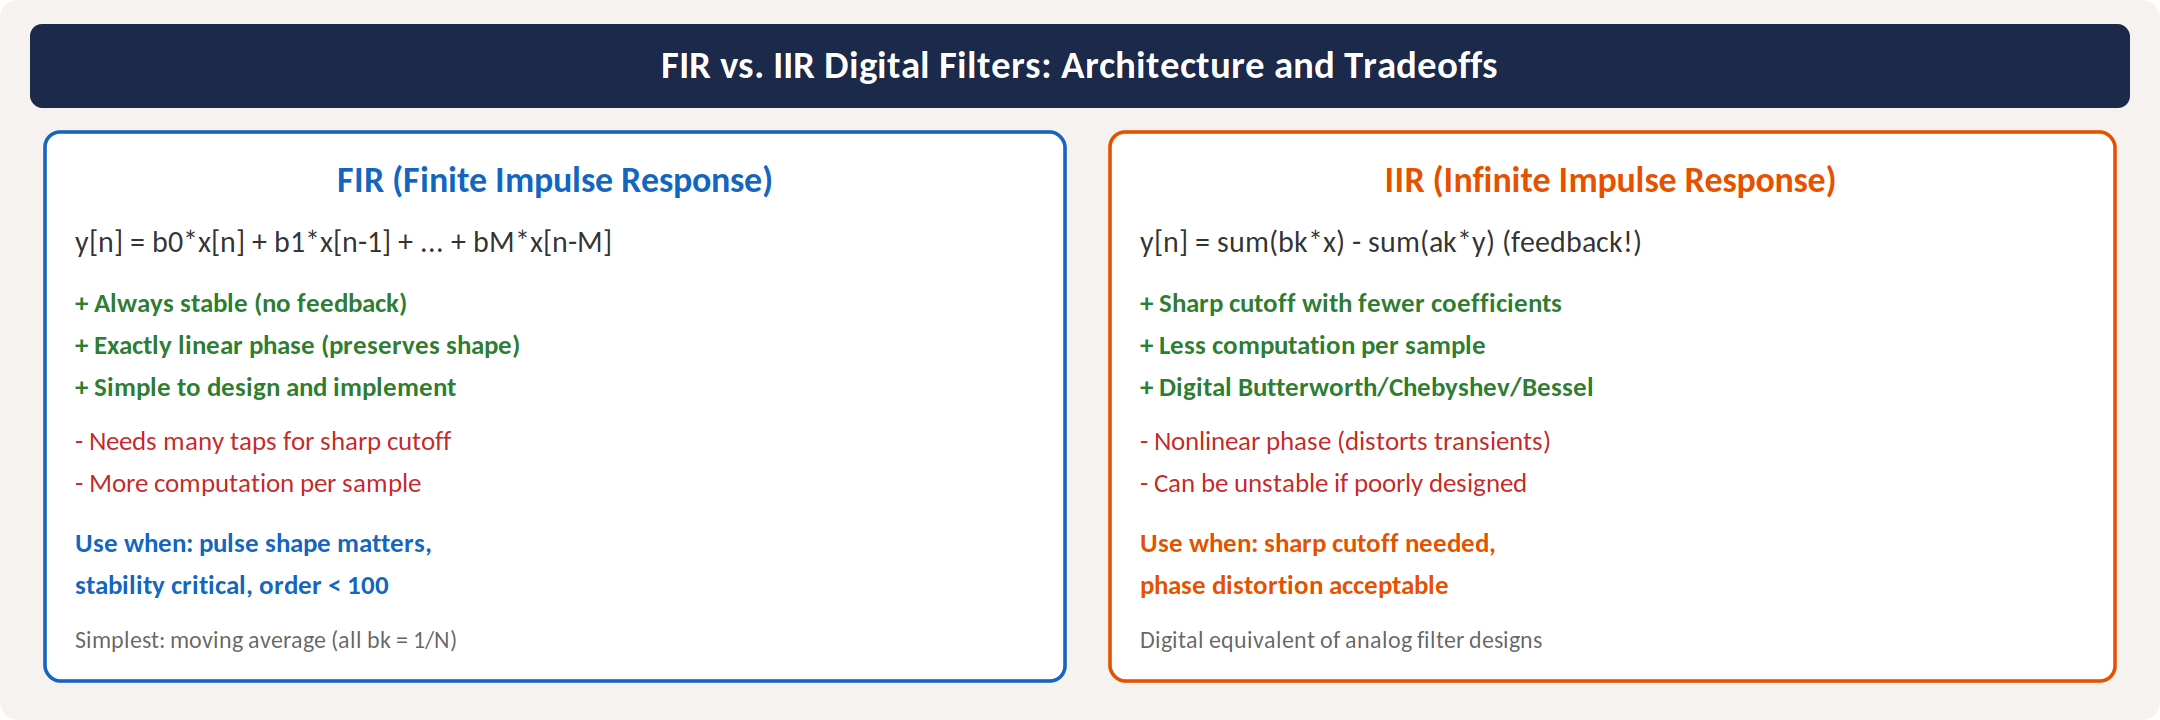
\includegraphics[width=\textwidth]{fig_fir_vs_iir.png}
\caption{FIR vs.\ IIR digital filters. FIR is always stable with linear phase; IIR achieves sharper cutoff with fewer coefficients but has nonlinear phase and stability risk. Use FIR when pulse shape matters; IIR when sharp cutoff matters.}
\label{fig:fir_iir}
\end{figure}

\begin{tipbox}[FIR vs.\ IIR Decision]
Use FIR when: linear phase is required (preserving pulse shape), stability is critical, or the filter order is manageable ($<$100 taps). Use IIR when: sharp cutoff is needed with minimal computation, phase distortion is acceptable, or you are implementing a digital equivalent of a known analog filter.
\end{tipbox}

\section{Practical Digital Filtering in LabVIEW}
LabVIEW provides the \texttt{Filter Express VI} (interactive design) and the \texttt{IIR/FIR Filter Design} toolkit (programmatic). Specify: filter type (LP/HP/BP/BS), response (Butterworth/Chebyshev/Bessel), order, and cutoff frequency. The VI outputs filtered data; apply it to your DAQ signal chain.


\section{Advantages of Digital Filters}
Exact coefficients (no component tolerances), easy parameter changes in software, can implement impractical analog types (perfect linear phase, adaptive), no drift, can process stored data offline. Limitation: cannot undo aliasing.

\section{Moving Average Filter}
$y[n] = (1/M)\sum_{k=0}^{M-1}x[n-k]$. FIR with all coefficients $= 1/M$. Bandwidth $\approx 0.44 f_s/M$. Nulls at $f_s/M$ and multiples. Excellent for smoothing slowly varying signals. Poor frequency selectivity. In LabVIEW: shift register + Mean function, or Filter Express VI with Smoothing.

\section{FIR Filter Design}
Design by windowing: specify ideal response, compute inverse DFT (sinc for LP), truncate to $M$ points, multiply by window (Hamming, Blackman, Kaiser). Window choice determines transition width vs.\ stopband attenuation tradeoff.

Order $M$ determines sharpness. Estimate: $M \approx 3.3/(\Delta f/f_s)$ for Hamming window. Group delay: $M/2$ samples. A symmetric FIR has exactly linear phase, preserving transient shapes.

\section{IIR Filter Design}
$y[n] = \sum b_k x[n-k] - \sum a_k y[n-k]$. Feedback gives efficiency: a 4th-order Butterworth needs only 9 coefficients (vs.\ 100+ FIR taps). Design: analog prototype $\to$ bilinear transform $\to$ digital coefficients. Implement as cascaded biquad sections for numerical stability.

\begin{warningbox}[Fixed-Point Stability]
On MCUs without FPU, IIR coefficients quantized to 16-bit integers can cause instability for $Q > 10$ or cutoff $< f_s/100$. Always simulate with actual precision before deploying.
\end{warningbox}

\section{Selection Guide}
Smooth noisy DC data $\to$ moving average. Sharp cutoff $\to$ IIR Butterworth/Chebyshev. Preserve pulse shape $\to$ FIR linear phase or IIR Bessel. Remove single frequency $\to$ IIR notch. Adaptive $\to$ FIR LMS (advanced).


\section{Implementation in LabVIEW}
LabVIEW provides several digital filter options. The \textbf{Filter Express VI} offers one-click configuration: select filter type (LP, HP, BP, BS), response (Butterworth, Chebyshev, Bessel, Elliptic), order, and cutoff frequency. It processes the entire waveform in one call.

For real-time filtering (one sample at a time in a control loop), use the \textbf{IIR Filter with Initialize} or implement the filter manually using shift registers. The manual approach provides explicit control over filter state initialization, anti-windup interaction, and coefficient precision.

\subsection{Filter Testing Methodology}
Test your digital filter with known inputs: (1) Apply a step function (constant array) to verify DC gain and settling behavior. (2) Apply a sine wave at the cutoff frequency to verify the $-3$\,dB attenuation. (3) Apply a sine wave at $10\times$ cutoff to verify stopband rejection. (4) Apply white noise and verify the output spectrum shows the expected rolloff.

\section{Decimation and Interpolation Filters}
When reducing sample rate (decimation), a digital LP filter at the new Nyquist frequency must precede the sample-rate reduction to prevent aliasing. This ``decimation filter'' is typically implemented as an FIR filter. For efficient multistage decimation (e.g., 100:1), cascade several smaller decimation stages (e.g., 10:1 $\to$ 10:1), each with its own anti-alias filter. This requires fewer total filter taps than a single-stage approach.

\section{Adaptive Filters (Overview)}
Adaptive filters automatically adjust their coefficients to minimize an error signal. The Least Mean Squares (LMS) algorithm is the simplest: $w[n+1] = w[n] + \mu \cdot e[n] \cdot x[n]$, where $\mu$ is the step size. Applications: noise cancellation (use a reference noise signal to adaptively subtract noise from the measurement), echo cancellation, and system identification. While beyond the scope of MEGN 300 labs, understanding that such filters exist prepares you for graduate-level signal processing.
\section{Detailed FIR Design Example}
Design a 50-tap FIR low-pass filter with cutoff at 100\,Hz for data sampled at 1\,kS/s.

\textbf{Step 1}: normalized cutoff $f_c/f_N = 100/500 = 0.2$ (where $f_N = f_s/2$).

\textbf{Step 2}: the ideal LP impulse response is a sinc function: $h[n] = \sin(2\pi \times 0.2 \times (n - 25))/((\pi(n-25))$ for $n = 0, \ldots, 49$ (centered at $n = 25$ for a 50-tap filter).

\textbf{Step 3}: apply a Hamming window: $w[n] = 0.54 - 0.46\cos(2\pi n/49)$. The windowed coefficients are $b[n] = h[n] \times w[n]$.

\textbf{Step 4}: normalize so the DC gain is unity: divide all $b[n]$ by their sum.

The resulting filter has a $-3$\,dB cutoff at approximately 100\,Hz, transition bandwidth of $\sim$40\,Hz (80--120\,Hz), and stopband rejection of $\sim$$-53$\,dB (Hamming window property). The group delay is exactly 25 samples (2.5\,ms at 1\,kS/s).

In LabVIEW, this entire design is accomplished by the ``FIR Windowed Coefficients'' VI: specify the sampling rate, cutoff frequency, number of taps, and window type. The VI outputs the coefficient array, which you wire to the ``FIR Filter'' VI.

\section{IIR Biquad Implementation}
The biquad (second-order section) is the building block of IIR filter implementation:
\begin{equation}
H(z) = \frac{b_0 + b_1 z^{-1} + b_2 z^{-2}}{1 + a_1 z^{-1} + a_2 z^{-2}}
\end{equation}
The difference equation:
\begin{equation}
y[n] = b_0 x[n] + b_1 x[n-1] + b_2 x[n-2] - a_1 y[n-1] - a_2 y[n-2]
\end{equation}

Implementation in LabVIEW or C requires two memory locations (shift registers or variables) for past inputs ($x[n-1]$, $x[n-2]$) and two for past outputs ($y[n-1]$, $y[n-2]$). A 4th-order filter uses two cascaded biquads, each with its own set of 5 coefficients ($b_0, b_1, b_2, a_1, a_2$). The biquad cascade is numerically more stable than a single high-order section because each biquad's coefficients are close to 1.0, minimizing quantization sensitivity.

\subsection{Direct Form II Transposed}
For floating-point implementation, the Direct Form II Transposed structure provides the best numerical properties. Instead of separate input and output delay lines, it uses a single state vector:
\begin{verbatim}
  y[n] = b0*x[n] + s1
  s1 = b1*x[n] - a1*y[n] + s2
  s2 = b2*x[n] - a2*y[n]
\end{verbatim}
This requires only two state variables per biquad section, minimizing memory and maximizing numerical precision.

\section{Real-Time Filtering in Control Loops}
When a digital filter is used inside a control loop (e.g., filtering the sensor signal before feeding it to the PID controller), the filter introduces delay that affects control stability.

\textbf{FIR delay}: an $M$-tap FIR introduces exactly $M/2$ samples of group delay. For $M = 50$ at 1\,kS/s: 25\,ms delay. At the controller's crossover frequency, this delay contributes phase lag: $\phi = 360 \times f \times 0.025$ degrees. At $f = 10$\,Hz: $\phi = 90^\circ$, which is likely to destabilize the loop.

\textbf{IIR delay}: varies with frequency. A 2nd-order Butterworth at $f_c = 100$\,Hz introduces approximately 3\,ms of group delay at 10\,Hz (much less than the equivalent FIR). This is why IIR filters are preferred in control applications where phase delay matters.

\textbf{Design rule}: the filter's group delay at the controller's crossover frequency should contribute less than $20^\circ$ of phase lag. For a 10\,Hz crossover: max delay $= 20/(360 \times 10) = 5.6$\,ms. A 2nd-order IIR at $f_c = 50$\,Hz easily meets this; a 50-tap FIR at 1\,kS/s does not.

\section{Notch Filter Design}
A notch (band-reject) filter removes a single frequency. The second-order IIR notch:
\begin{equation}
H(z) = \frac{1 - 2\cos(\omega_0 T_s)z^{-1} + z^{-2}}{1 - 2r\cos(\omega_0 T_s)z^{-1} + r^2 z^{-2}}
\end{equation}
where $\omega_0 = 2\pi f_{\text{notch}}$ and $r$ controls the notch width (typical: $r = 0.95$--$0.99$; closer to 1 = narrower notch). For 60\,Hz rejection at $f_s = 1000$\,S/s: $\omega_0 T_s = 2\pi \times 60/1000 = 0.3770$\,rad.

Cascading two notch filters (at 60\,Hz and 120\,Hz) removes the fundamental and first harmonic of mains interference. Three notches (60, 120, 180\,Hz) handle most situations.

\section{Comb Filters}
A comb filter rejects a fundamental frequency and all its harmonics simultaneously:
\begin{equation}
H(z) = \frac{1 - z^{-D}}{1 - \alpha z^{-D}}
\end{equation}
where $D = f_s/f_{\text{fundamental}}$ (must be an integer) and $\alpha$ controls the notch width. For rejecting 60\,Hz and all harmonics at $f_s = 600$\,S/s: $D = 10$. The filter has nulls at 60, 120, 180, \ldots, 300\,Hz. This is more efficient than cascading individual notch filters. The tradeoff: it also removes any real signal content at these frequencies.
\section{Comparison: LabVIEW Filter VIs}
LabVIEW offers several filtering VIs, each suited to different applications:

\textbf{Filter Express VI}: one-click configuration (type, response, order, cutoff). Processes the entire waveform in one call. Best for: offline analysis of acquired data, quick prototyping.

\textbf{IIR Filter VI}: takes a waveform and returns a filtered waveform. Supports Butterworth, Chebyshev, Bessel, and Elliptic responses. Offers ``reverse filtering'' option that applies the filter forward and backward, canceling phase distortion (zero-phase filtering, only for offline data).

\textbf{FIR Windowed Filter VI}: generates and applies an FIR filter. Specify taps, cutoff, window type. Best for: linear-phase requirements, real-time filtering with known group delay.

\textbf{Median Filter VI}: replaces each sample with the median of the surrounding $N$ samples. Excellent for removing spike noise (salt-and-pepper noise) while preserving edges. Not a frequency-domain filter; useful for preprocessing before FFT or control.

\textbf{Savitzky-Golay Filter}: fits a local polynomial to each data neighborhood. Smooths noise while preserving peak shapes and widths. Widely used in chromatography and spectroscopy. Available in LabVIEW's Signal Processing palette.

\section{Filter Transient Behavior}
Every digital filter has a startup transient: the output is invalid for the first $M$ samples (where $M$ is the filter order for IIR or the number of taps for FIR). During this time, the filter's internal state is filling with data. Discard (or ignore) the first $M$ output samples. In a control loop, initialize the filter states with the first measured value (not zero) to minimize the startup transient.

For IIR filters, the transient decays exponentially with a time constant related to the pole locations. A narrow-band IIR filter (low cutoff relative to $f_s$, or high $Q$) has a long transient that can persist for hundreds of samples. Plan your acquisition duration to include the transient plus the required steady-state data.
\section{Zero-Phase Filtering}
Conventional (causal) digital filters introduce phase distortion: different frequencies experience different delays. For time-domain analysis (peak detection, rise time measurement, waveform comparison), this phase distortion can be problematic. \textbf{Zero-phase filtering} eliminates phase distortion by applying the filter twice: once forward and once backward (time-reversed). The magnitude response is squared (doubled in dB), but the phase distortion cancels exactly.

In LabVIEW, enable ``Reverse Filtering'' in the IIR Filter VI options. In MATLAB: \texttt{filtfilt(b,a,x)}. Important: zero-phase filtering is only possible for offline data (you need the entire signal before filtering). It cannot be used in real-time control because the backward pass requires future samples.

\section{Implementing Filters on Microcontrollers}
For embedded systems (ESP32, Arduino, STM32) without floating-point units, digital filters must be implemented in fixed-point arithmetic. Key considerations:

\textbf{Coefficient quantization}: round filter coefficients to the available precision (typically 16 or 32 bits). Simulate the quantized filter and verify that the frequency response still meets specifications and that no instability occurs.

\textbf{Overflow protection}: intermediate calculations can exceed the word size. Use 32-bit accumulators for 16-bit data, or saturating arithmetic that clips at the maximum value instead of wrapping around.

\textbf{Execution time}: each filter tap requires one multiply-accumulate (MAC) operation. A 50-tap FIR at 10\,kS/s requires 500,000 MACs/s. An ARM Cortex-M4 at 168\,MHz executes $\sim$168 million MACs/s (with DSP instructions), leaving ample headroom. An 8-bit AVR at 16\,MHz can manage $\sim$4 million MACs/s, limiting filter complexity.

\textbf{Circular buffer}: the shift register for past samples is efficiently implemented as a circular buffer (ring buffer): a fixed-size array with a pointer that wraps around, avoiding the need to physically shift data.

\section{Practical Filter Selection Flowchart}
(1) Is the signal DC or slowly varying ($f < 1$\,Hz)? $\to$ Moving average ($M = 10$--100).

(2) Do you need sharp frequency cutoff? $\to$ IIR Butterworth (default) or Chebyshev (maximum sharpness).

(3) Is pulse shape or rise time critical? $\to$ FIR with linear phase.

(4) Do you need to remove 60\,Hz without affecting other frequencies? $\to$ IIR notch at 60\,Hz ($r = 0.97$).

(5) Do you need to remove 60\,Hz and all harmonics? $\to$ Comb filter ($D = f_s/60$).

(6) Is the noise source unknown or changing? $\to$ Adaptive FIR (LMS) with a reference noise signal.

(7) Is the filter inside a feedback control loop? $\to$ Low-order IIR (2nd order max) to minimize phase lag.
\section{Windowed FIR Design: Detailed Procedure}
The windowed FIR design method is the most intuitive and widely used approach:

\textbf{Step 1: Specify the ideal frequency response.} For a low-pass filter with cutoff $f_c$ (normalized to $f_N = f_s/2$): $H_d(f) = 1$ for $|f| \leq f_c$, $H_d(f) = 0$ for $|f| > f_c$.

\textbf{Step 2: Compute the ideal impulse response.} The inverse Fourier transform of the ideal rectangular frequency response is a sinc function: $h_d[n] = \sin(2\pi f_c (n - M/2)) / (\pi(n - M/2))$ for $n = 0, 1, \ldots, M$, where $M$ is the filter order (number of taps minus 1). At $n = M/2$: $h_d[M/2] = 2f_c$ (by L'H\^opital's rule).

\textbf{Step 3: Apply the window.} Multiply the truncated impulse response by a window function: $h[n] = h_d[n] \cdot w[n]$. The window tapers the coefficients to zero at the ends, which suppresses the sidelobes in the frequency response (at the cost of widening the transition band).

\textbf{Step 4: Normalize.} Divide all coefficients by their sum to ensure unity DC gain: $h_{\text{norm}}[n] = h[n] / \sum_k h[k]$.

\subsection{Window Function Selection}
\begin{table}[htbp]\centering\small
\begin{tabularx}{\textwidth}{l X c c}
\toprule
\textbf{Window} & \textbf{Characteristics} & \textbf{Min.\ stopband (dB)} & \textbf{Trans.\ BW ($\times f_s/M$)} \\
\midrule
Rectangular & Narrowest main lobe, worst sidelobes & $-21$ & 0.9 \\
Hamming & Good all-around choice & $-53$ & 3.3 \\
Hanning & Slightly wider, better sidelobes & $-44$ & 3.1 \\
Blackman & Excellent sidelobes, wide transition & $-74$ & 5.5 \\
Kaiser ($\beta = 8$) & Adjustable tradeoff via $\beta$ & $-80$ & 5.0 \\
\bottomrule
\end{tabularx}
\caption{FIR window function comparison. Transition bandwidth determines the minimum filter order needed for a given sharpness.}
\end{table}

The Kaiser window is the most versatile: the parameter $\beta$ adjusts the sidelobe-to-mainlobe tradeoff continuously. For a target stopband attenuation $A_s$ (dB): $\beta = 0.1102(A_s - 8.7)$ for $A_s > 50$\,dB. The required order: $M = (A_s - 8)/(2.285 \times \Delta\omega)$ where $\Delta\omega = 2\pi\Delta f/f_s$ is the normalized transition width.

\section{Equiripple (Parks-McClellan) FIR Design}
For demanding applications, the Parks-McClellan algorithm designs an FIR filter that minimizes the maximum error between the desired and actual frequency response (minimax criterion). This produces an equiripple response: the error oscillates with equal amplitude across both the passband and stopband.

Advantages over windowed design: for a given filter order, the equiripple design achieves either narrower transition band or greater stopband rejection. The improvement is significant for high-order filters ($M > 50$).

In MATLAB: \texttt{b = firpm(M, [0 fp fs 1], [1 1 0 0])} where \texttt{fp} is the passband edge and \texttt{fs} is the stopband edge (both normalized to Nyquist). In LabVIEW: the ``Equiripple FIR'' VI in the Signal Processing palette.

\section{Multirate Filter Structures}
\subsection{Polyphase Decomposition}
For efficient decimation, the FIR filter can be decomposed into $M$ polyphase subfilters, each operating at the lower output rate. This reduces computation by exactly $M\times$ compared to filtering at the input rate and then discarding samples. The polyphase structure is the standard implementation in commercial DAQ systems and audio equipment.

\subsection{Cascaded Integrator-Comb (CIC) Filter}
A computationally efficient decimation filter that requires no multiplications (only additions and subtractions). The CIC consists of $N$ integrator stages followed by $N$ comb (differentiator) stages with a rate change between them. The frequency response has a sinc$^N$ shape, providing good rejection of aliased components near multiples of the output rate. CIC filters are the first stage of decimation in sigma-delta ADCs, reducing the sample rate by factors of 32--256 before a more precise FIR filter handles the final shaping.

\section{Adaptive Filtering: The LMS Algorithm}
The Least Mean Squares (LMS) adaptive filter automatically adjusts its coefficients to minimize the error between its output and a desired signal. The update rule:
\begin{equation}
\mathbf{w}[n+1] = \mathbf{w}[n] + \mu \cdot e[n] \cdot \mathbf{x}[n]
\end{equation}
where $\mathbf{w}$ is the coefficient vector, $\mu$ is the step size (learning rate), $e[n] = d[n] - y[n]$ is the error, and $\mathbf{x}$ is the input vector.

The most common application: \textbf{noise cancellation}. A reference microphone captures the ambient noise. The adaptive filter models the acoustic path from the noise source to the primary microphone. The filter's output is subtracted from the primary signal, canceling the noise while preserving the desired signal. This is the technology behind noise-canceling headphones.

In instrumentation, adaptive filtering can cancel vibration interference, remove 60\,Hz hum using a reference from the power line, or compensate for time-varying sensor characteristics.
\section{Real-Time Filter Implementation Checklist}
Before deploying a digital filter in a control or monitoring system, verify:

(1) \textbf{Coefficient precision}: simulate the filter with the actual numerical precision of the target platform (32-bit float, 64-bit double, or 16-bit fixed). Compare the frequency response to the ideal design. If the response deviates: use biquad cascade (not direct form), increase precision, or redesign with less aggressive specifications.

(2) \textbf{Initialization}: set the filter state (shift register values) to the first sample value, not zero. Initializing to zero causes a startup transient as the filter ``fills'' with data. Initializing to the first sample assumes the signal was at this value for all past time, which produces a much smaller transient.

(3) \textbf{Overflow}: for fixed-point, verify that intermediate accumulator values do not exceed the word size. Use saturation arithmetic (clip at max/min) rather than wraparound arithmetic (which produces catastrophic sign flips).

(4) \textbf{Latency}: measure the actual output delay from input change to output response. For FIR: exactly $M/2$ samples. For IIR: frequency-dependent (measure at the frequency of interest).

(5) \textbf{Computational load}: measure the execution time of the filter operation. Verify it completes within the sample period ($T_s = 1/f_s$). If not: reduce the filter order, increase the sample period, or use a faster processor.

\section{Filter Banks}
A \textbf{filter bank} splits a signal into multiple frequency bands, each processed independently. The octave filter bank (used in acoustic measurement and vibration analysis) divides the spectrum into bands whose bandwidth is proportional to center frequency: 1\,Hz band at 1\,Hz, 10\,Hz band at 10\,Hz, 100\,Hz band at 100\,Hz, etc. This matches human perception (which is logarithmic in frequency) and the characteristics of many physical processes.

In MEGN~300, filter banks are encountered in the context of 1/3-octave analysis for noise measurement (ANSI S1.11) and vibration severity assessment (ISO 10816). LabVIEW's Sound and Vibration Toolkit includes octave analysis VIs.

\section{Hilbert Transform Filter}
A Hilbert transform filter produces a 90-degree phase shift at all frequencies, converting a cosine to a sine (and vice versa) without changing the amplitude. Combined with the original signal, it produces the \textbf{analytic signal}, whose magnitude is the instantaneous envelope and whose phase derivative is the instantaneous frequency.

FIR implementation: the ideal Hilbert transform impulse response is $h[n] = 2\sin^2(\pi n/2)/(\pi n)$ for $n \neq 0$, $h[0] = 0$. Truncate and window (like any FIR design). Typical order: 31--63 taps.

Application in instrumentation: envelope detection for bearing fault diagnosis, demodulation of AM signals, and instantaneous frequency tracking for speed-varying machinery.
\section{Practice Questions}
\begin{enumerate}[leftmargin=1.5em]
\item Design a 10-point moving average filter for a signal sampled at 1\,kS/s. What is the effective cutoff frequency? By how much does it reduce random noise?
\item Explain why a moving average filter is poor at removing a specific frequency (like 60\,Hz) compared to a notch filter.
\item You need a digital low-pass filter with a cutoff of 100\,Hz, linear phase, and a sampling rate of 10\,kS/s. Would you choose FIR or IIR? Why?
\end{enumerate}

\subsection{Answers}
\begin{enumerate}[leftmargin=1.5em]
\item A 10-point moving average has its first null at $f_s/N = 1000/10 = 100$\,Hz. The $-3$\,dB frequency is approximately $0.443 \times f_s/N = 44.3$\,Hz. Noise reduction: $\sqrt{10} = 3.16\times$ ($10$\,dB).
\item A moving average has a $\sin(x)/x$ frequency response with broad, shallow notches at multiples of $f_s/N$. Unless $f_s/N$ happens to equal exactly 60\,Hz, the 60\,Hz component is only partially attenuated. A notch filter, by contrast, has a very narrow, deep rejection specifically at 60\,Hz (and its harmonics if designed correctly).
\item FIR. The linear-phase requirement rules out IIR filters, which inherently have nonlinear phase. A FIR filter with symmetric coefficients provides exactly linear phase. At $f_s = 10$\,kS/s with $f_c = 100$\,Hz, the filter will need many taps (perhaps 200--500 for a sharp cutoff), but this is computationally feasible in LabVIEW on a modern PC.
\end{enumerate}


% ################################################################
% PART III: ELECTRONICS FOR INSTRUMENTATION
% ################################################################
\part{Electronics for Instrumentation}

\chapter{Circuit Fundamentals}

This chapter reviews the core electrical concepts that underpin every topic in Parts~III and IV. If you are comfortable with Ohm's Law, Kirchhoff's Laws, and basic RC/RL transients, this chapter serves as a concise reference. If these ideas are new or rusty, work through the examples before moving on to amplifiers and power electronics.

\section{Voltage, Current, Resistance, and Power}

\textbf{Voltage} ($V$, measured in volts) is the electrical potential difference between two points. It is the ``pressure'' that pushes charge through a circuit. \textbf{Current} ($I$, measured in amperes) is the rate of charge flow: $I = dQ/dt$. Conventional current flows from higher to lower potential (positive to negative); electron flow is opposite. \textbf{Resistance} ($R$, measured in ohms, $\Omega$) quantifies how strongly a material opposes current flow. \textbf{Power} ($P$, measured in watts) is the rate of energy transfer: $P = VI$. In a resistor, $P = I^2 R = V^2/R$.

\begin{keyconceptbox}[Ohm's Law]
The voltage across a resistor is proportional to the current through it:
\begin{equation}
V = IR \qquad \Leftrightarrow \qquad I = \frac{V}{R} \qquad \Leftrightarrow \qquad R = \frac{V}{I}
\end{equation}
This is the single most-used equation in electronics. It applies to any purely resistive element: resistors, wire, heating elements, and the on-resistance of a MOSFET switch.
\end{keyconceptbox}

\textbf{Conductance} ($G = 1/R$, measured in siemens, S) is the reciprocal of resistance. It is convenient when combining parallel resistances: $G_{\text{total}} = G_1 + G_2 + \cdots$.

\textbf{Energy} ($E$, measured in joules) is power integrated over time: $E = P \cdot t$. A 100\,W heater running for 60\,s dissipates $100 \times 60 = 6000$\,J. Battery capacity is often stated in watt-hours (Wh) or milliamp-hours (mAh): a 2000\,mAh battery at 3.7\,V stores $2.0 \times 3.7 = 7.4$\,Wh $= 26{,}640$\,J.

\section{Kirchhoff's Laws}

Gustav Kirchhoff formulated two conservation laws that, together with Ohm's Law, allow you to solve any circuit.

\subsection{Kirchhoff's Current Law (KCL)}
The algebraic sum of currents entering a node is zero:
\begin{equation}
\sum I_{\text{in}} = \sum I_{\text{out}}
\end{equation}
Current is conserved. Whatever flows into a junction must flow out. If three wires meet at a node carrying 2\,A, 3\,A, and $I_3$, then $I_3 = -(2+3) = -5$\,A (5\,A flowing out).

\subsection{Kirchhoff's Voltage Law (KVL)}
The algebraic sum of voltages around any closed loop is zero:
\begin{equation}
\sum V_{\text{loop}} = 0
\end{equation}
Energy is conserved. The voltage rises (sources) must equal the voltage drops (resistors, loads) around any closed path.

\begin{examplebox}[KVL Applied: Series Resistor Circuit]
A 12\,V supply drives two series resistors: $R_1 = 4\,\text{k}\Omega$ and $R_2 = 8\,\text{k}\Omega$. Apply KVL: $V_s - V_{R1} - V_{R2} = 0$. The current is $I = V_s/(R_1 + R_2) = 12/12{,}000 = 1\,\text{mA}$. Then $V_{R1} = 1\,\text{mA} \times 4\,\text{k}\Omega = 4\,\text{V}$ and $V_{R2} = 8\,\text{V}$. Check: $12 - 4 - 8 = 0$. KVL is satisfied.
\end{examplebox}

\section{Series and Parallel Circuits}

\subsection{Series Combination}
Components in series carry the same current. Resistances add directly:
\begin{equation}
R_{\text{series}} = R_1 + R_2 + \cdots + R_n
\end{equation}
The total resistance is always larger than any individual resistor. Voltage divides among the resistors in proportion to their resistance.

\subsection{Parallel Combination}
Components in parallel share the same voltage across their terminals. Conductances add (equivalently, reciprocals of resistance add):
\begin{equation}
\frac{1}{R_{\text{parallel}}} = \frac{1}{R_1} + \frac{1}{R_2} + \cdots + \frac{1}{R_n}
\end{equation}
For two resistors: $R_{\text{parallel}} = R_1 R_2 / (R_1 + R_2)$. The total resistance is always less than the smallest individual resistor.

\begin{tipbox}[Quick Parallel Calculation]
Two equal resistors in parallel give half the resistance: $R_{\text{parallel}} = R/2$. A 10\,k$\Omega$ resistor in parallel with a 1\,k$\Omega$ resistor gives $10 \times 1 / (10 + 1) = 909\,\Omega$, which is close to the smaller resistor alone. In parallel combinations, the smallest resistor dominates.
\end{tipbox}

\section{Voltage Dividers}

The voltage divider is the most common subcircuit in instrumentation. Two series resistors connected across a source produce an output voltage at their junction:
\begin{equation}
V_{\text{out}} = V_{\text{in}} \cdot \frac{R_2}{R_1 + R_2}
\end{equation}

\textbf{Applications in MEGN 300}: scaling a sensor output to match the ADC input range (0--3.3\,V for the ESP32), creating a reference voltage, and biasing op-amp circuits.

\begin{warningbox}[Loading a Voltage Divider]
A voltage divider only produces the calculated voltage if the load draws negligible current compared to the divider current. Rule of thumb: the load resistance should be at least 10$\times$ the divider output resistance ($R_1 \| R_2$). If not, the load acts as a parallel resistor on $R_2$ and pulls the output voltage down. Use a voltage follower (op-amp buffer) to isolate a high-impedance divider from a low-impedance load.
\end{warningbox}

\begin{examplebox}[ThermoRig: 12\,V Sensor to 3.3\,V ADC]
A pressure sensor outputs 0--10\,V. The ESP32 ADC accepts 0--3.3\,V. Design: $V_{\text{out}} = V_{\text{in}} \times R_2/(R_1 + R_2)$. Target ratio: $3.3/10 = 0.33$. Choose $R_1 = 20\,\text{k}\Omega$, $R_2 = 10\,\text{k}\Omega$: output $= 10 \times 10/30 = 3.33$\,V. Divider current: $10/30{,}000 = 0.33$\,mA (low, does not load the sensor). Add a 100\,nF capacitor across $R_2$ to filter high-frequency noise.
\end{examplebox}

\section{Thevenin and Norton Equivalent Circuits}

Any linear circuit, no matter how complex, can be reduced to a single voltage source in series with a single resistance (Thevenin) or a single current source in parallel with a single resistance (Norton).

\textbf{Thevenin equivalent}: $V_{Th}$ = open-circuit voltage at the output terminals; $R_{Th}$ = resistance seen from the output terminals with all independent sources set to zero (voltage sources shorted, current sources opened).

\textbf{Norton equivalent}: $I_N = V_{Th}/R_{Th}$; $R_N = R_{Th}$.

\textbf{Why this matters for instrumentation}: every sensor has an output impedance ($R_{Th}$). If you connect a low-impedance load (like a multimeter on the current range, or an ADC with a low input impedance), the output voltage drops from $V_{Th}$ because of the voltage drop across $R_{Th}$. This is the root cause of loading errors in measurement systems.

\section{Capacitors and Inductors}

\subsection{Capacitors}
A capacitor stores energy in an electric field between two conductive plates separated by a dielectric:
\begin{equation}
Q = CV, \qquad I = C\frac{dV}{dt}, \qquad E = \frac{1}{2}CV^2
\end{equation}
Capacitance $C$ is measured in farads (F). Practical values: pF (high-frequency coupling), nF (decoupling, filtering), $\mu$F (bulk energy storage, timing). A capacitor opposes changes in voltage; it passes AC and blocks DC. Impedance: $Z_C = 1/(2\pi f C)$, which decreases with frequency.

\textbf{Types used in MEGN~300}: ceramic (100\,pF--10\,$\mu$F, low ESR, ideal for decoupling), electrolytic (1\,$\mu$F--10{,}000\,$\mu$F, polarized, bulk energy storage), and tantalum (0.1--100\,$\mu$F, low ESR, compact but voltage-sensitive).

\subsection{Inductors}
An inductor stores energy in a magnetic field generated by current flowing through a coil:
\begin{equation}
V = L\frac{dI}{dt}, \qquad E = \frac{1}{2}LI^2
\end{equation}
Inductance $L$ is measured in henrys (H). An inductor opposes changes in current; it passes DC and blocks AC. Impedance: $Z_L = 2\pi f L$, which increases with frequency. Motor windings, solenoid coils, and relay coils are all inductors. This is why they produce voltage spikes when switched (Chapter~14).

\section{RC and RL Time Constants}

\subsection{RC Circuit}
A resistor and capacitor in series produce an exponential charging or discharging response. The time constant is:
\begin{equation}
\tau = RC
\end{equation}
After one time constant, the capacitor charges to 63.2\% of the final value. After $5\tau$, it reaches 99.3\% (practically complete). The step response is:
\begin{equation}
V_C(t) = V_{\text{final}} \left(1 - e^{-t/\tau}\right) \quad \text{(charging)}, \qquad V_C(t) = V_{\text{initial}} \cdot e^{-t/\tau} \quad \text{(discharging)}
\end{equation}

\textbf{Applications}: low-pass filtering ($R$ in series, $C$ to ground; cutoff $f_c = 1/(2\pi RC)$), debouncing a mechanical switch ($\tau \approx 10$\,ms), and ADC input filtering to reduce noise.

\begin{examplebox}[Anti-Alias Filter for DAQ]
You need a low-pass filter with $f_c = 1$\,kHz to prevent aliasing before a 10\,kS/s ADC. Choose $C = 10$\,nF. Then $R = 1/(2\pi f_c C) = 1/(2\pi \times 1000 \times 10 \times 10^{-9}) = 15.9\,\text{k}\Omega$. Use a standard 16\,k$\Omega$ resistor ($f_c = 995$\,Hz, close enough). This is a single-pole, $-20$\,dB/decade rolloff. For steeper attenuation, use higher-order filters (Chapter~11).
\end{examplebox}

\subsection{RL Circuit}
A resistor and inductor in series produce an analogous exponential response with time constant:
\begin{equation}
\tau = L/R
\end{equation}
Current rises as $I(t) = I_{\text{final}}(1 - e^{-t/\tau})$ when voltage is applied, and decays as $I(t) = I_{\text{initial}} \cdot e^{-t/\tau}$ when the source is removed. RL time constants are critical for understanding relay pull-in time (the coil current must reach the hold-in threshold) and flyback voltage spikes (the energy stored as $\frac{1}{2}LI^2$ must dissipate when the switch opens).

\section{AC Circuit Fundamentals}

\subsection{Impedance}
In AC circuits, resistance generalizes to impedance ($Z$), which has both magnitude and phase. For a resistor: $Z_R = R$ (purely real, voltage and current in phase). For a capacitor: $Z_C = 1/(j\omega C)$ (current leads voltage by 90$^\circ$). For an inductor: $Z_L = j\omega L$ (current lags voltage by 90$^\circ$). Impedances combine like resistances: in series they add, in parallel the reciprocals add. Ohm's Law applies using impedance: $V = IZ$.

\subsection{RMS Values}
Alternating signals are characterized by their root-mean-square (RMS) value, which represents the equivalent DC value that delivers the same average power to a resistive load:
\begin{equation}
V_{\text{RMS}} = \frac{V_{\text{peak}}}{\sqrt{2}} \approx 0.707 \cdot V_{\text{peak}} \qquad \text{(sinusoidal signals only)}
\end{equation}
US household power: $V_{\text{peak}} = 170$\,V, $V_{\text{RMS}} = 120$\,V. Power calculations always use RMS: $P = V_{\text{RMS}}^2/R = I_{\text{RMS}}^2 R$.

\subsection{Decibels}
Signal magnitudes in instrumentation are often expressed in decibels (dB), a logarithmic ratio:
\begin{equation}
\text{Gain (dB)} = 20 \log_{10}\left(\frac{V_{\text{out}}}{V_{\text{in}}}\right) = 10 \log_{10}\left(\frac{P_{\text{out}}}{P_{\text{in}}}\right)
\end{equation}
A gain of $+6$\,dB $\approx$ doubling the voltage. A gain of $-3$\,dB $\approx$ voltage reduced to 0.707 (half-power point, used to define filter cutoff frequencies). A gain of $-20$\,dB $=$ voltage reduced by a factor of 10. Decibels are additive through a signal chain: a $+20$\,dB amplifier followed by a $-6$\,dB attenuator gives $+14$\,dB overall.

\section{Grounding and Ground Loops}

\textbf{Ground} is the reference node (0\,V) against which all voltages are measured. In theory, ground is a single point at 0\,V everywhere. In practice, ground conductors have nonzero resistance and carry return currents, creating small voltage differences between ``ground'' points in different parts of the circuit.

A \textbf{ground loop} occurs when two or more ground connections create a closed loop that can pick up magnetically induced currents (from nearby motors, transformers, or switching supplies), generating noise on the signal ground. Ground loops are one of the most common sources of measurement noise in instrumentation labs.

\begin{tipbox}[Star Grounding]
Connect all subsystem grounds to a single point (the star point) near the power supply, rather than daisy-chaining ground connections from one module to the next. Keep signal ground (sensors, ADC) and power ground (motors, relays) on separate conductors that meet only at the star point. This prevents motor return currents from flowing through the sensor ground path and corrupting measurements.
\end{tipbox}

\section{Practical Component Selection}

\subsection{Resistor Color Code}
Through-hole resistors use colored bands to encode their value. The standard 4-band code works as follows: the first two bands are significant digits, the third band is the multiplier (number of zeros), and the fourth band indicates tolerance. Read the bands starting from the end closest to one lead (the tolerance band is usually spaced slightly farther from the others).

\begin{center}
\begin{tabular}{lccl}
\toprule
\textbf{Color} & \textbf{Digit} & \textbf{Multiplier} & \textbf{Tolerance} \\
\midrule
Black   & 0 & $\times 1$         & --- \\
Brown   & 1 & $\times 10$        & $\pm 1\%$ \\
Red     & 2 & $\times 100$       & $\pm 2\%$ \\
Orange  & 3 & $\times 1{,}000$   & --- \\
Yellow  & 4 & $\times 10{,}000$  & --- \\
Green   & 5 & $\times 100{,}000$ & $\pm 0.5\%$ \\
Blue    & 6 & $\times 1{,}000{,}000$ & $\pm 0.25\%$ \\
Violet  & 7 & $\times 10{,}000{,}000$ & $\pm 0.1\%$ \\
Gray    & 8 & ---                & $\pm 0.05\%$ \\
White   & 9 & ---                & --- \\
Gold    & --- & $\times 0.1$     & $\pm 5\%$ \\
Silver  & --- & $\times 0.01$    & $\pm 10\%$ \\
\bottomrule
\end{tabular}
\end{center}

\textbf{5-band resistors} (precision, 1\% or better) use three significant digits, a multiplier, and a tolerance band. The reading process is the same: first three bands are digits, fourth is multiplier, fifth is tolerance.

\begin{examplebox}[Reading Resistor Color Codes]
\textbf{4-band}: Brown--Black--Orange--Gold $= 10 \times 1{,}000 = 10\,\text{k}\Omega$, $\pm 5\%$. The range is 9.5\,k$\Omega$ to 10.5\,k$\Omega$.

\textbf{4-band}: Red--Violet--Red--Gold $= 27 \times 100 = 2.7\,\text{k}\Omega$, $\pm 5\%$.

\textbf{5-band}: Brown--Red--Black--Brown--Brown $= 120 \times 10 = 1.2\,\text{k}\Omega$, $\pm 1\%$.

\textbf{Common mnemonic} (digit order 0--9): ``Better Be Right Or Your Great Big Venture Goes Wrong'' (Black, Brown, Red, Orange, Yellow, Green, Blue, Violet, Gray, White).
\end{examplebox}

\begin{tipbox}[SMD Resistor Markings]
Surface-mount resistors use a numeric code instead of color bands. The 3-digit code (e.g., ``103'') uses the first two digits as significant figures and the third as the number of zeros: $103 = 10 \times 10^3 = 10\,\text{k}\Omega$. The 4-digit code (e.g., ``4702'') uses three significant digits: $4702 = 470 \times 10^2 = 47\,\text{k}\Omega$. ``R'' indicates a decimal point: ``4R7'' $= 4.7\,\Omega$. Very small SMD packages (0402 and below) often have no marking at all; keep them in labeled bags or tape reels to avoid confusion.
\end{tipbox}

\subsection{Resistor Tolerance and Standard Values}
Resistors come in standard value series (E12, E24, E96) spaced logarithmically. The E12 series (10\% tolerance) has 12 values per decade: 10, 12, 15, 18, 22, 27, 33, 39, 47, 56, 68, 82. The E24 series (5\%) has 24 values. E96 (1\%) has 96 values. When designing a voltage divider or filter, choose the nearest standard value and verify the circuit still meets specifications at the tolerance extremes.

\subsection{Power Rating}
Every resistor has a maximum power dissipation. Standard through-hole resistors: 1/4\,W. Verify: $P = I^2R$ or $P = V^2/R$ at worst-case operating conditions. If the dissipation exceeds the rating, the resistor overheats, changes value, and eventually fails (sometimes by catching fire).

\subsection{Capacitor Voltage Rating}
Every capacitor has a maximum working voltage. Exceeding it causes dielectric breakdown (shorts, explosion for electrolytics). Rule of thumb: derate by 50\% for reliability (use a 25\,V cap on a 12\,V rail). Electrolytic capacitors are polarized; reversing polarity causes catastrophic failure.

\subsection{Wire Gauge Reference (AWG)}
American Wire Gauge (AWG) is the standard for specifying wire size. Smaller AWG numbers indicate thicker wire with higher current capacity. The following table covers the gauges most commonly used in MEGN~300 projects:

\begin{center}
\begin{tabular}{cccl}
\toprule
\textbf{AWG} & \textbf{Diameter (mm)} & \textbf{Max Current (A)} & \textbf{Typical Use} \\
\midrule
30 & 0.25 & 0.5  & Wire-wrap, fine signal wiring \\
28 & 0.32 & 0.8  & Ribbon cable, breadboard jumpers \\
26 & 0.40 & 1.3  & Ribbon cable, light signal wiring \\
24 & 0.51 & 2.1  & Standard signal and sensor wiring \\
22 & 0.64 & 3.0  & General purpose hookup wire \\
20 & 0.81 & 5.0  & Power wiring, LED strips \\
18 & 1.02 & 7.5  & Motor power, moderate loads \\
16 & 1.29 & 10   & High-current motor, battery leads \\
14 & 1.63 & 15   & High-power supply, automotive \\
12 & 2.05 & 20   & Household branch circuits (US) \\
\bottomrule
\end{tabular}
\end{center}

Current ratings above are approximate for chassis wiring in open air (single conductor, 30\degC{} ambient). Bundled wires in conduit or cable should be derated by 20--40\%. When in doubt, go one gauge thicker.

\begin{warningbox}[Stranded vs. Solid Wire]
Use \textbf{stranded wire} for any connection that moves, flexes, or is subject to vibration (motor leads, connections to moving parts, cables between enclosures). Solid wire work-hardens and breaks after repeated flexing. Use \textbf{solid wire} only for permanent, stationary connections (breadboard jumpers, point-to-point wiring on perfboard). Never use solid wire for connections to motors, servos, or any moving mechanism.
\end{warningbox}

\subsection{SI Prefixes and Unit Conversions}
Instrumentation spans many orders of magnitude. Memorize these prefixes:

\begin{center}
\begin{tabular}{ccll}
\toprule
\textbf{Prefix} & \textbf{Symbol} & \textbf{Factor} & \textbf{Common Usage} \\
\midrule
pico  & p  & $10^{-12}$ & Capacitance (pF), charge \\
nano  & n  & $10^{-9}$  & Capacitance (nF), time (ns) \\
micro & $\mu$ & $10^{-6}$ & Voltage ($\mu$V), current ($\mu$A), time ($\mu$s) \\
milli & m  & $10^{-3}$  & Voltage (mV), current (mA), time (ms) \\
---   & ---  & $10^{0}$ & Base unit (V, A, $\Omega$, s, Hz) \\
kilo  & k  & $10^{3}$   & Resistance (k$\Omega$), frequency (kHz) \\
mega  & M  & $10^{6}$   & Resistance (M$\Omega$), frequency (MHz) \\
giga  & G  & $10^{9}$   & Frequency (GHz) \\
\bottomrule
\end{tabular}
\end{center}

\begin{warningbox}[Case Sensitivity in Unit Prefixes]
Lowercase ``m'' means milli ($10^{-3}$). Uppercase ``M'' means mega ($10^{6}$). Confusing them changes a value by a factor of one billion. A 4.7\,m$\Omega$ resistor (milliohm, a current-sense shunt) is very different from a 4.7\,M$\Omega$ resistor (megaohm, a high-impedance input bias resistor). Similarly, ``mA'' is milliamps and ``MA'' is megaamps. Always double-check the case when reading datasheets and specifications.
\end{warningbox}

\subsection{Common Schematic Symbols}
Knowing how to read a schematic is a prerequisite for building, debugging, and documenting any circuit. The following symbols appear throughout this course and in component datasheets:

\textbf{Passive components}: resistor (zigzag or rectangle), capacitor (two parallel lines; polarized electrolytic adds a curved line for the negative plate), inductor (series of loops or bumps), fuse (thin line with a break or ``S'' shape).

\textbf{Semiconductors}: diode (triangle pointing into a bar; current flows in the triangle direction, from anode to cathode), LED (diode with arrows representing emitted light), Zener diode (diode with bent bar ends), NPN BJT (arrow on emitter pointing away from base), PNP BJT (arrow on emitter pointing toward base), N-channel MOSFET (arrow on body diode pointing inward, gate on left side), P-channel MOSFET (arrow pointing outward).

\textbf{Sources and references}: DC voltage source (circle with $+$/$-$), AC voltage source (circle with sine wave), ground symbol (three horizontal lines of decreasing length, or a triangle pointing down), chassis ground (three diagonal lines).

\textbf{Active components}: op-amp (triangle with $+$ and $-$ inputs and one output), comparator (same symbol as op-amp but context indicates comparison function).

\subsection{Multimeter Usage Quick Reference}
The digital multimeter (DMM) is the most-used instrument in MEGN~300. Correct usage prevents both measurement errors and equipment damage.

\textbf{Voltage measurement} (DC or AC): set the dial to V; connect probes in parallel across the component or nodes of interest. The DMM presents very high input impedance ($>$1\,M$\Omega$) and draws negligible current.

\textbf{Current measurement}: set the dial to A or mA; move the red probe to the current jack (usually a separate terminal). Connect the meter in series: break the circuit and insert the meter into the break so all current flows through it. The DMM presents very low impedance ($<$1\,$\Omega$) when measuring current.

\textbf{Resistance measurement}: set the dial to $\Omega$. Disconnect the component from the circuit (de-energize first!). Connect probes across the component. The DMM sends a small known current through the component and measures the resulting voltage to compute resistance.

\textbf{Continuity}: set to the continuity/beep mode (diode symbol or speaker icon). Touch probes to two points. The meter beeps if resistance is below a threshold (typically $<$50\,$\Omega$), indicating an electrical connection.

\begin{warningbox}[The Current-Mode Dead-Short Trap]
If you leave the multimeter in current mode (low impedance, probes in the current jacks) and connect it in parallel across a voltage source, the meter becomes a near-short-circuit. This blows the meter's internal fuse (best case) or damages the meter and the circuit (worst case). After every current measurement, move the red probe back to the voltage jack and switch the dial to voltage mode. This is the single most common multimeter damage mode in the MEGN~300 lab.
\end{warningbox}

\subsection{Breadboard Layout and Conventions}
Breadboards are used for rapid prototyping before committing to a soldered or PCB design. Internal connections run as follows: the two long rails along the top and bottom edges are bus strips (typically used for power and ground, marked with red/blue or $+$/$-$ lines). The central rows of five-hole groups are connected horizontally within each group but not across the center channel. The center channel separates the two halves and is sized to straddle a DIP IC package.

\textbf{Best practices}: run power ($+$) on the red rail and ground on the blue rail, both on the same side of the board for short return paths. Place ICs straddling the center channel. Use short, flat jumper wires (color-coded: red for power, black for ground, other colors for signals). Keep wires close to the board surface to reduce noise pickup and make the circuit readable. Label every IC and major node with a small sticky note.

\textbf{Limitations}: breadboard contact resistance is 0.01--0.1\,$\Omega$ per connection (adds up over long signal paths), stray capacitance is 2--5\,pF between adjacent rows (limits high-frequency performance to $<$1\,MHz), and connections loosen over time (intermittent failures). Never deploy a breadboard as a final product.

\begin{keyconceptbox}[Requirements Mapping: Circuit Parameters to Shall Statements]
Circuit analysis directly generates testable requirements. ``The input stage voltage divider shall scale the 0--10\,V sensor output to 0--3.3\,V with an accuracy of $\pm$2\%.'' ``The signal ground and power ground shall connect at a single star point within 50\,mm of the main power entry connector.'' ``All resistors in the signal conditioning path shall be 1\% tolerance (E96 series) or better.'' ``Bulk decoupling capacitors shall have a voltage rating at least 1.5$\times$ the rail voltage.''
\end{keyconceptbox}

\section{Practice Questions}
\begin{enumerate}[leftmargin=1.5em]
\item A circuit has a 9\,V battery driving three resistors: $R_1 = 1\,\text{k}\Omega$ in series with the parallel combination of $R_2 = 2\,\text{k}\Omega$ and $R_3 = 3\,\text{k}\Omega$. Find the total current from the battery and the voltage across each resistor.
\item An RC low-pass filter uses $R = 10\,\text{k}\Omega$ and $C = 100$\,nF. What is the $-3$\,dB cutoff frequency? How long does the capacitor take to reach 99\% of a step input?
\item A Thevenin analysis of a sensor circuit yields $V_{Th} = 2.5$\,V and $R_{Th} = 5\,\text{k}\Omega$. You connect it to an ADC with 1\,M$\Omega$ input impedance. What voltage does the ADC actually read? What if the ADC input impedance were only 10\,k$\Omega$?
\end{enumerate}

\subsection{Answers}
\begin{enumerate}[leftmargin=1.5em]
\item $R_{2\|3} = (2 \times 3)/(2 + 3) = 1.2\,\text{k}\Omega$. $R_{\text{total}} = 1.0 + 1.2 = 2.2\,\text{k}\Omega$. $I = 9/2200 = 4.09$\,mA. $V_{R1} = 4.09\,\text{mA} \times 1\,\text{k}\Omega = 4.09$\,V. $V_{R2\|R3} = 4.09\,\text{mA} \times 1.2\,\text{k}\Omega = 4.91$\,V. Check: $4.09 + 4.91 = 9.0$\,V (KVL satisfied).
\item $f_c = 1/(2\pi RC) = 1/(2\pi \times 10{,}000 \times 100 \times 10^{-9}) = 159$\,Hz. For 99\% of final value: $5\tau = 5 \times RC = 5 \times 10{,}000 \times 100 \times 10^{-9} = 5$\,ms.
\item With 1\,M$\Omega$ load: $V_{\text{ADC}} = 2.5 \times 10^6/(5000 + 10^6) = 2.488$\,V (0.5\% loading error, negligible). With 10\,k$\Omega$ load: $V_{\text{ADC}} = 2.5 \times 10{,}000/(5000 + 10{,}000) = 1.667$\,V (33\% loading error, severe). This illustrates why ADC input impedance matters and why a buffer amplifier may be needed.
\end{enumerate}


\chapter{Amplifiers}

\section{Why Amplification?}
Many sensors produce millivolt or microvolt signals (thermocouples: $\sim$40\,$\mu$V/\degC{}; strain gauges: $\sim$2\,mV/V at full scale). ADCs work best when the signal spans most of their input range. Amplification bridges this gap, improving resolution and SNR.

\section{Operational Amplifier (Op-Amp) Fundamentals}
An ideal op-amp has infinite gain, infinite input impedance, zero output impedance, and infinite bandwidth. Real op-amps approximate this well enough for most instrumentation.

\subsection{Inverting Amplifier}
\begin{equation}
V_{\text{out}} = -\frac{R_f}{R_{\text{in}}} V_{\text{in}}, \qquad G = -\frac{R_f}{R_{\text{in}}}
\end{equation}
The $-$ sign means the output is inverted. Input impedance equals $R_{\text{in}}$; this can load a high-impedance sensor.

\subsection{Non-Inverting Amplifier}
\begin{equation}
V_{\text{out}} = \left(1 + \frac{R_f}{R_g}\right) V_{\text{in}}, \qquad G = 1 + \frac{R_f}{R_g}
\end{equation}
No inversion. Very high input impedance (the op-amp's input impedance, typically $>$1\,G$\Omega$). Preferred for sensor interfacing.

\subsection{Voltage Follower (Buffer)}
Non-inverting amplifier with $G = 1$ ($R_f = 0$, $R_g = \infty$). Provides impedance transformation: high input impedance, low output impedance. Use between a high-impedance sensor and a low-impedance load (ADC input, cable driver).

\subsection{Differential Amplifier}
\begin{equation}
V_{\text{out}} = G (V_+ - V_-)
\end{equation}
Amplifies the difference between two inputs while rejecting the common-mode voltage (noise, ground offsets). Critical for bridge circuits (strain gauges, RTDs) and any measurement in electrically noisy environments.

\section{Instrumentation Amplifiers}
A specialized differential amplifier with three op-amps that provides: very high input impedance on both inputs, precisely settable gain with a single resistor ($R_G$), and very high Common-Mode Rejection Ratio (CMRR). The gain equation (for a standard 3-op-amp INA):
\begin{equation}
G = 1 + \frac{2R}{R_G}
\end{equation}
Common ICs: INA128, AD620, INA333. CMRR typically $>$100\,dB.

\begin{figure}[htbp]
\centering
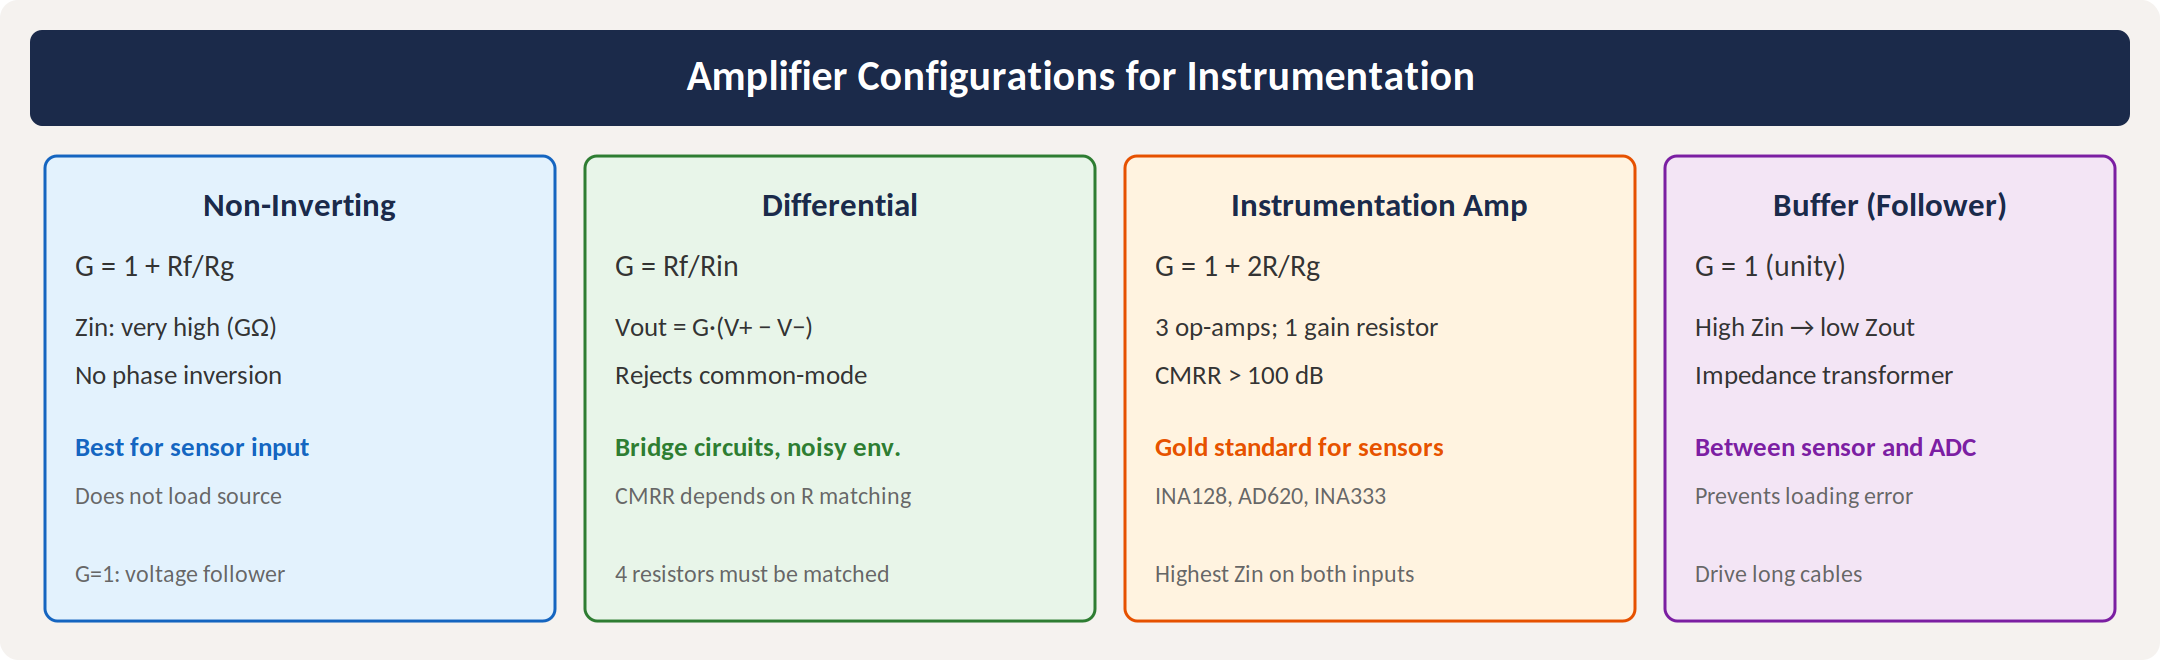
\includegraphics[width=\textwidth]{fig_amplifier_types.png}
\caption{Four amplifier configurations for instrumentation. The instrumentation amplifier (INA) is the gold standard for sensor interfacing.}
\label{fig:amps}
\end{figure}

\begin{keyconceptbox}[Requirements Mapping: Amplifier to Shall-Statements]
\begin{itemize}[nosep,leftmargin=1.5em]
\item ``Measure strain gauge bridge output (0--10\,mV) with a 0--5\,V ADC'' $\to$ AMP-REQ: Amplifier gain shall be 500 $\pm$ 0.1\%. Amplifier CMRR shall be $\geq$ 100\,dB to reject 60\,Hz common-mode noise.
\item ``Sensor output impedance is 10\,k$\Omega$'' $\to$ AMP-REQ: Amplifier input impedance shall be $\geq$ 100\,M$\Omega$ (10,000:1 ratio to avoid loading error $>$ 0.01\%).
\end{itemize}
\end{keyconceptbox}


\section{Amplifier Noise}
Real amplifiers add noise to the signal. Two key specifications:

\textbf{Input-referred voltage noise} ($e_n$): specified in nV/$\sqrt{\text{Hz}}$. Total noise voltage $= e_n \times \sqrt{\text{bandwidth}}$. For an INA128: $e_n \approx 8$\,nV/$\sqrt{\text{Hz}}$.

\textbf{Input-referred current noise} ($i_n$): specified in pA/$\sqrt{\text{Hz}}$. Generates noise across the source impedance: $V_n = i_n \times R_s$. High source impedance (thermocouples, piezo sensors) makes current noise dominant.

\textbf{Total input-referred noise}:
\begin{equation}
V_{n,\text{total}} = \sqrt{e_n^2 + (i_n R_s)^2 + 4k_B T R_s} \times \sqrt{\text{BW}}
\end{equation}
where the third term is thermal (Johnson) noise from the source resistance.

\begin{tipbox}[Choosing an Amplifier for Low-Noise Applications]
For low source impedance ($<$1\,k$\Omega$, e.g., strain gauge bridges): choose a low $e_n$ amplifier (INA128, AD8221). For high source impedance ($>$100\,k$\Omega$, e.g., piezo sensors): choose a low $i_n$ amplifier (INA116, OPA129; FET-input types). Always calculate total noise and compare to your signal level to verify adequate SNR.
\end{tipbox}


\begin{warningbox}[Mandate: Use Differential Mode for All Millivolt-Level Signals]
When a sensor is physically separated from the DAQ (even by 1 meter of cable), the sensor's ``ground'' and the DAQ's ``ground'' are at different potentials. This ground offset (often 10--100\,mV from building wiring) adds directly to your measurement. For a thermocouple producing 1\,mV, a 50\,mV ground offset is a 50$\times$ error. \textbf{Solution}: always configure the NI~DAQ in Differential mode for millivolt-level signals (thermocouples, strain gauge bridges, low-output sensors). Differential mode measures the voltage \emph{between} the two signal wires, rejecting the common-mode ground offset. In NI~MAX, select ``Differential'' (not ``RSE'') when configuring analog input channels.
\end{warningbox}

\section{Signal Conditioning Chains}
A complete signal conditioning chain for a resistive sensor:

\begin{enumerate}[leftmargin=1.5em]
\item \textbf{Bridge excitation}: precision voltage or current source drives the Wheatstone bridge.
\item \textbf{Instrumentation amplifier}: amplifies the differential bridge output (typically 100--1000$\times$) while rejecting common-mode voltage.
\item \textbf{Low-pass filter}: removes high-frequency noise and provides anti-aliasing. Cutoff frequency set to $\leq 0.4 f_s$.
\item \textbf{Voltage offset/scaling}: shifts and scales the signal to match the ADC input range (0--5\,V or $\pm$10\,V).
\item \textbf{ADC}: digitizes the conditioned signal.
\end{enumerate}

\begin{examplebox}[ThermoRig: Complete Signal Chain for Strain Measurement]
A 350\,$\Omega$ strain gauge in a quarter-bridge (\textbf{ThermoRig Variant: Strain Measurement} --- this example demonstrates the signal chain design process for a resistive sensor, complementing the thermocouple-based ThermoRig) with $V_{ex} = 5$\,V. At 1000\,$\mu\epsilon$: $\Delta V = V_{ex} \times GF \times \epsilon / 4 = 5 \times 2.1 \times 0.001 / 4 = 2.625$\,mV. Signal chain: INA128 at $G = 500$ ($V_{out} = 1.31$\,V), followed by a 2nd-order Butterworth LP at 500\,Hz, feeding a 16-bit ADC ($\pm$5\,V range). ADC resolution at sensor: $10/(65536 \times 500) = 0.305\,\mu$V $= 0.116\,\mu\epsilon$. Noise: INA128 noise ($8\,\text{nV}/\sqrt{\text{Hz}} \times \sqrt{500} = 179$\,nV input-referred) $\to$ referred to strain: $179\,\text{nV} / (5 \times 2.1 / 4) = 0.068\,\mu\epsilon$. Total: well within a $\pm$5\,$\mu\epsilon$ requirement.
\end{examplebox}


\section{Why Amplification Is Necessary}
Sensor outputs are often too small for the ADC. A Type K thermocouple at 100\,\degC{} produces only 4.1\,mV. An NI USB-6001 on $\pm$10\,V has 1.22\,mV LSB, meaning the TC signal spans only 3--4 bits. Amplification by 500--1000$\times$ utilizes the full 14-bit range.

\section{Op-Amp Fundamentals}
Key real-world limitations: \textbf{Input offset voltage ($V_{os}$)}: 0.1--5\,mV. At gain 1000, a 1\,mV offset becomes 1\,V. Use precision or auto-zero op-amps. \textbf{Input bias current ($I_b$)}: nA to pA. Creates voltage offsets across high-impedance sources. Match impedances or use FET-input. \textbf{GBW}: gain $\times$ bandwidth is constant. 1\,MHz GBW gives 1000$\times$ gain only to 1\,kHz. \textbf{Slew rate}: max output change rate (V/$\mu$s). For 5\,V at 10\,kHz: need $\geq$0.31\,V/$\mu$s.

\section{Amplifier Configurations}
\textbf{Non-inverting}: $G = 1 + R_f/R_g$. High input impedance. Default for sensors.

\textbf{Inverting}: $G = -R_f/R_i$. Input impedance $= R_i$. Use when inversion is acceptable.

\textbf{Buffer}: $G = 1$. Converts high-impedance source to low-impedance output.

\textbf{Differential}: $V_o = (R_f/R_i)(V_2 - V_1)$. CMRR limited by resistor matching ($\sim$60\,dB for 0.1\% resistors).

\section{Instrumentation Amplifier (INA)}
Three-op-amp topology: two input buffers + difference amplifier. $G = 1 + 2R/R_G$. CMRR $> 100$\,dB. Very high input impedance ($>10^{10}\,\Omega$). Gain set by single resistor. The gold standard for sensor interfacing.

\begin{examplebox}[ThermoRig: Complete Signal Chain]
TC produces 0--8.2\,mV (0--200\,\degC{}). DAQ accepts 0--5\,V. Required gain: $G \approx 600$. INA128 ($R = 49.4$\,k$\Omega$): $R_G = 98.8\text{k}/(600-1) = 165\,\Omega$. Use 162\,$\Omega$ standard, $G = 611$. CMRR of 120\,dB rejects 50\,mV ground offset. Signal chain: TC $\to$ INA128 ($G = 611$) $\to$ Sallen-Key LP (40\,Hz) $\to$ NI USB-6001 (diff, 0--5\,V, 100\,S/s).
\end{examplebox}

\section{Common Mistakes}
(1) No decoupling capacitors (100\,nF at each power pin). (2) Input exceeds common-mode range. (3) Driving capacitive loads without series resistor (causes oscillation). (4) Gain maps signal beyond ADC range (clipping).


\section{Reading Op-Amp Datasheets}
The datasheet is the most important document for amplifier design. Key sections to examine:

\textbf{Absolute maximum ratings}: voltages and currents that must never be exceeded. Exceeding these destroys the device permanently. Always design with margin.

\textbf{Electrical characteristics table}: input offset voltage ($V_{os}$), input bias current ($I_b$), open-loop gain ($A_{ol}$), CMRR, GBW product, slew rate. These are specified at particular conditions (supply voltage, temperature).

\textbf{Typical performance curves}: plots of key parameters vs.\ frequency, temperature, and supply voltage. The ``Open-Loop Gain vs.\ Frequency'' plot determines the usable gain-bandwidth. The ``CMRR vs.\ Frequency'' plot shows that CMRR degrades at high frequencies, which is critical for rejecting EMI.

\textbf{Application circuits}: the manufacturer's recommended configurations, including component values and PCB layout tips.

\section{PCB Layout for Low-Noise Amplifiers}
Poor layout can undo careful circuit design. Key rules: (1) Keep traces short between sensor input and amplifier. (2) Route analog traces away from digital and power traces. (3) Use a continuous ground plane under the amplifier. (4) Place decoupling capacitors within 5\,mm of power pins. (5) Use Kelvin connections for precision resistors (separate current and voltage traces). (6) Enclose the sensitive input area with a guard ring (a trace connected to the non-inverting input potential) to intercept leakage currents.

\section{Signal Conditioning Chain Design Example}
For a full Wheatstone bridge strain gauge system: (1) Bridge excitation: REF5050 (5.000\,V precision reference). (2) First stage: INA128 with $G = 100$ (maps $\pm$20\,mV bridge output to $\pm$2\,V). (3) Second stage: 4th-order Sallen-Key Butterworth LP at 100\,Hz (anti-alias for 1\,kS/s DAQ). (4) Buffer: unity-gain buffer (OPA2277) to drive the DAQ input. (5) DAQ: NI USB-6001, differential input, $\pm$5\,V range, 1\,kS/s. Total system noise: dominated by the INA128's $e_n = 8$\,nV/$\sqrt{\text{Hz}}$ over 100\,Hz bandwidth: $V_n = 8 \times \sqrt{100} = 80$\,nV input-referred, or $80 \times 100 = 8$\,$\mu$V at the ADC, well below the 1.22\,mV LSB.
\section{Op-Amp Selection Guide}
With thousands of op-amps available, selection can be overwhelming. Use this decision tree for MEGN~300 applications:

\textbf{General purpose (non-critical)}: TL072 (JFET input, low cost, GBW = 3\,MHz). Good for buffering, non-inverting amplification of volt-level signals, and filter stages where noise is not the limiting factor.

\textbf{Precision DC measurement}: OPA2277 ($V_{os} = 10\,\mu$V, low drift, low noise). For strain gauge amplification, thermocouple signal conditioning, and any application where DC accuracy matters.

\textbf{Low noise}: OPA1612 ($e_n = 1.1$\,nV/$\sqrt{\text{Hz}}$). For hydrophone preamplifiers, high-impedance sensor buffering, and applications where the noise floor limits measurement resolution.

\textbf{High speed}: OPA657 (GBW = 1.6\,GHz, slew rate = 700\,V/$\mu$s). For photodiode transimpedance amplifiers, high-frequency signal conditioning, and wideband measurements. Requires careful PCB layout.

\textbf{Rail-to-rail, single supply}: MCP6022 (operates on 2.5--5.5\,V, rail-to-rail I/O). For battery-powered portable instruments and 3.3\,V MCU-compatible signal conditioning.

\section{INA Design Details}
\subsection{Gain Resistor Selection}
The INA128's gain equation $G = 1 + 49.4\text{k}\Omega / R_G$ means that very high gains require very small $R_G$. At $G = 1000$: $R_G = 49.4\,\Omega$. At this value, the resistor's lead resistance and contact resistance (especially on a breadboard) can contribute significant gain error. Solution: use a precision ($\leq$0.1\%), low-TCR metal film resistor soldered directly to the INA's $R_G$ pins. Never use a potentiometer for $R_G$ (the wiper resistance fluctuates).

\subsection{Input Bias Current Path}
The INA128's input bias current ($\pm$2\,nA typical) must have a DC return path to ground. If the sensor is AC-coupled (capacitor in series) or the source is floating (isolated thermocouple), the bias current has no path, and the output saturates to the rail. Solution: add high-value resistors (1--10\,M$\Omega$) from each input to ground, providing the bias current path while maintaining high common-mode impedance.

\subsection{Reference Pin}
The INA128's output is referenced to the voltage on its REF pin (pin 5). For single-supply operation, connect REF to mid-supply (2.5\,V from a precision reference) to center the output swing. For bipolar operation, connect REF to ground. If REF is driven by a noisy source, the noise appears directly at the output.

\section{Signal Chain Design Methodology}
A systematic approach to designing the complete signal conditioning chain:

\textbf{Step 1: Define the input and output.} Input: sensor output range (e.g., $-10$ to $+40$\,mV for a thermocouple at 0--200\,\degC{}). Output: ADC input range (e.g., 0--5\,V).

\textbf{Step 2: Calculate required gain.} $G = V_{\text{ADC,range}} / V_{\text{sensor,range}} = 5000\,\text{mV}/50\,\text{mV} = 100$.

\textbf{Step 3: Add offset to shift the signal.} The sensor output includes negative values ($-10$\,mV at 0\,\degC{}). After $100\times$ gain: $-1$\,V (cannot be measured by a 0--5\,V ADC). Add an offset of $+1$\,V after amplification, or bias the INA's REF pin to $+1$\,V.

\textbf{Step 4: Design the anti-alias filter.} For 100\,S/s sample rate and 10\,Hz signal bandwidth: 2nd-order Sallen-Key Butterworth at $f_c = 40$\,Hz. This provides $-24$\,dB attenuation at $f_s/2 = 50$\,Hz, adequate for 14-bit.

\textbf{Step 5: Verify the noise budget.} Compute the total output noise and compare to the ADC's LSB. If the noise exceeds 0.5\,LSB, reduce the bandwidth, increase the gain (to use more of the ADC range), or select a lower-noise amplifier.

\textbf{Step 6: Simulate, build, test.} Use SPICE simulation (LTspice is free) to verify the design before building. After building, measure the actual gain, offset, frequency response, and noise, and compare to the design.

\section{Differential vs.\ Single-Ended Signal Routing}
\textbf{Single-ended}: one signal wire and a ground return. Simple but susceptible to ground noise. Use for volt-level signals from low-impedance sources over short distances ($<$30\,cm).

\textbf{Differential}: two signal wires (no ground reference). Rejects common-mode noise. Use for millivolt signals, long cable runs, and noisy environments. The INA at the receiving end converts differential to single-ended.

\textbf{Rule of thumb}: if the sensor output is less than 100\,mV, or the cable is longer than 1\,m, or the environment contains motors/power electronics, use differential signal routing with an INA.
\section{Practical Amplifier Troubleshooting}
\textbf{Output saturated at positive rail}: (1) check power supply connections (is $V+$ actually connected?), (2) check for open feedback path ($R_f$ disconnected = infinite gain = rail), (3) check input common-mode range (input voltage too high for the op-amp).

\textbf{Output saturated at negative rail}: (1) check that $V-$ supply is connected, (2) check for reversed input polarity (signal on $V-$ instead of $V+$ for non-inverting), (3) check for DC offset amplified to the rail.

\textbf{Output oscillates at high frequency (MHz range)}: (1) add decoupling capacitors (100\,nF ceramic at power pins), (2) check for capacitive load on output (add 100\,$\Omega$ series resistor), (3) verify the op-amp is unity-gain stable (some high-speed op-amps require minimum gain for stability).

\textbf{Output has excessive noise}: (1) check grounding (star ground, no ground loops), (2) check power supply decoupling, (3) verify the input is properly terminated (floating inputs pick up noise), (4) check for resistor values too high ($R > 100$\,k$\Omega$ increases thermal noise).

\textbf{Gain is wrong}: (1) measure actual resistor values with a multimeter (tolerance effects), (2) check for loading at the output (the next stage drawing current through $R_f$), (3) verify the op-amp has sufficient GBW for the gain and frequency.

\section{Precision Measurement Techniques}
\textbf{Chopper stabilization}: an auto-zero technique that periodically measures and corrects the offset voltage. The LTC2057 (chopper-stabilized) achieves $V_{os} = 0.5\,\mu$V and drift of 0.015\,$\mu$V/\degC{}. For thermocouple measurement where the sensor output is 41\,$\mu$V/\degC{}, a 0.5\,$\mu$V offset corresponds to only 0.012\,\degC{} of error, negligible.

\textbf{Guard rings}: for high-impedance circuits ($R > 1$\,G$\Omega$), PCB surface leakage can exceed the signal current. A guard ring (a PCB trace driven to the same potential as the high-impedance node, surrounding it on the PCB surface) intercepts leakage currents before they reach the sensitive input. Standard practice for pH meters, picoammeters, and charge amplifiers.

\textbf{Kelvin connections}: for precision resistance measurement, separate the current-carrying wires from the voltage-sensing wires. The current wires have IR drops across their resistance; the voltage-sensing wires carry no current (connected to high-impedance amplifier inputs) and therefore have no voltage error.

\section{INA Applications Beyond Temperature}
The instrumentation amplifier is used wherever a small differential signal must be extracted from a common-mode environment:

\textbf{Strain gauge bridges}: output is $\sim$2\,mV/V at full scale. INA gain of 200--1000 maps this to the ADC range.

\textbf{Current sensing} (high-side): a shunt resistor in the supply line produces a differential voltage proportional to current, riding on the full supply voltage as common-mode. The INA rejects the supply voltage and amplifies only the shunt voltage.

\textbf{Biomedical signals} (ECG, EMG): body-surface potentials are $\sim$1\,mV differential with $\sim$1\,V common-mode (from mains coupling to the body). INA with CMRR $> 100$\,dB rejects the mains interference.

\textbf{Thermocouple cold junction compensation}: the reference junction voltage ($\sim$1\,mV) must be measured differentially to reject the ground offset between the thermocouple and the compensation IC.
\section{Noise Analysis for Amplifier Circuits}
\subsection{Op-Amp Noise Model}
Every op-amp has two internal noise sources: a voltage noise source $e_n$ (in series with the non-inverting input) and a current noise source $i_n$ (flowing into each input). The total input-referred noise voltage depends on the source impedance $R_s$:
\begin{equation}
V_{n,\text{total}} = \sqrt{e_n^2 + (i_n R_s)^2 + 4k_B T R_s}
\end{equation}
The three terms represent: amplifier voltage noise, amplifier current noise flowing through the source impedance, and the source's own thermal noise. For low source impedance ($R_s < 1$\,k$\Omega$): $e_n$ dominates; choose a BJT-input op-amp (low $e_n$, e.g., OPA2277: 8\,nV/$\sqrt{\text{Hz}}$). For high source impedance ($R_s > 100$\,k$\Omega$): $i_n R_s$ dominates; choose a JFET-input op-amp (low $i_n$, e.g., OPA2132: 4\,fA/$\sqrt{\text{Hz}}$).

\subsection{Noise Gain}
The noise gain of an amplifier circuit is the gain experienced by the input-referred noise sources, which is \emph{not} always the same as the signal gain. For a non-inverting amplifier: noise gain $= 1 + R_f/R_g = $ signal gain. For an inverting amplifier: noise gain $= 1 + R_f/R_i$ but signal gain $= -R_f/R_i$. The noise gain is always $\geq 1$ and determines the amplifier's bandwidth (GBW/noise gain) and output noise.

\subsection{Noise Bandwidth}
The noise bandwidth of a filter is the bandwidth of an ideal rectangular filter that would pass the same total noise power. For a single-pole (first-order) system with $-3$\,dB frequency $f_{-3\text{dB}}$: noise bandwidth $= (\pi/2) f_{-3\text{dB}} = 1.57 f_{-3\text{dB}}$. For a second-order Butterworth: noise bandwidth $= 1.11 f_{-3\text{dB}}$. Use the noise bandwidth (not the $-3$\,dB bandwidth) when computing total noise from noise spectral density.

\section{Practical Circuit Construction}
\subsection{Breadboard vs.\ Protoboard vs.\ PCB}
\textbf{Breadboard}: acceptable for initial testing of digital circuits and proof-of-concept. Unacceptable for final analog signal conditioning: contact resistance varies (0.01--1\,$\Omega$), parasitic capacitance is high ($\sim$2\,pF between adjacent rows), and connections are unreliable under vibration. Maximum recommended use: circuits with signal levels $> 100$\,mV and frequencies $< 1$\,kHz.

\textbf{Protoboard} (solderable perfboard): adequate for most MEGN~300 final projects. Solder connections are permanent, low resistance ($< 1$\,m$\Omega$), and mechanically robust. Use point-to-point wiring with minimum wire length. Keep analog and digital sections physically separated with a ground plane (copper tape on the bottom side).

\textbf{Custom PCB}: best performance. Ground planes, controlled impedance traces, and optimized component placement minimize noise and parasitic effects. PCB fabrication services (JLCPCB, OSH~Park) produce 2-layer boards for \$2--\$5 with 5-day turnaround. For MEGN~301 projects requiring reliable, compact electronics: a custom PCB is strongly recommended.

\subsection{Decoupling Best Practices}
Every IC power pin needs a 100\,nF ceramic capacitor (C0G or X7R) placed within 5\,mm of the pin, connected to the nearest ground with the shortest possible trace. Additionally, place one 10\,$\mu$F electrolytic capacitor at each power rail entry point to the board. For op-amps operating above 1\,MHz: add a 1\,nF capacitor in parallel with the 100\,nF for high-frequency decoupling.

The decoupling capacitor provides local charge storage so that fast current transients (from the op-amp switching its output stage) are supplied locally rather than propagating through long power traces (which act as antennas, radiating EMI and injecting noise into adjacent circuits).

\section{Signal Chain Verification Checklist}
Before connecting the signal conditioning to the DAQ, verify each stage independently:

\begin{enumerate}[leftmargin=1.5em]
\item Power supply: correct voltage, low noise ($< 1$\,mV ripple on oscilloscope).
\item Zero input: short the amplifier input. Measure the output DC offset (should be $< V_{os} \times G$).
\item Known DC input: apply a precision voltage (from a calibrated source or voltage divider) and verify the output matches the expected gain.
\item Frequency response: sweep a sine wave from $0.1 f_c$ to $10 f_c$ and verify the gain and phase match the design.
\item Noise floor: short the input, measure the output RMS noise. Compare to the calculated noise budget.
\item Full-scale output: apply the maximum expected input and verify the output does not clip (stays within the ADC's input range).
\item Common-mode rejection (for INA): apply the same voltage to both inputs. The output should remain near zero (within the specified CMRR).
\end{enumerate}
\section{Op-Amp Non-Idealities: The Brutal Realities}
The preceding sections treat the op-amp as ideal (infinite gain, infinite bandwidth, zero offset). In practice, non-idealities are what destroy measurement accuracy. Understanding three key limitations prevents the most common student design failures.

\subsection{Gain-Bandwidth Product (GBW)}
An op-amp has finite open-loop gain that decreases with frequency at $-20$\,dB/decade above the dominant pole. The \textbf{Gain-Bandwidth Product} (GBW) is the frequency at which the open-loop gain equals 1 (0\,dB). For a TL072: GBW $= 3$\,MHz. For an OPA2277: GBW $= 1$\,MHz.

The maximum usable closed-loop bandwidth at gain $G$ is:
\begin{equation}
f_{\text{max}} = \frac{\text{GBW}}{G}
\end{equation}

For a non-inverting amplifier with $G = 1000$ using a TL072 (GBW $= 3$\,MHz): $f_{\text{max}} = 3000$\,Hz. Any signal above 3\,kHz is \emph{attenuated}, not amplified. A student expecting flat gain from DC to 10\,kHz will measure a signal that rolls off above 3\,kHz and be confused.

\begin{warningbox}[The Gain-Bandwidth Trap]
If you need $G = 1000$ with bandwidth to 10\,kHz, you need GBW $\geq 10{,}000 \times 1000 = 10$\,MHz (with $10\times$ margin: $\geq 100$\,MHz). No general-purpose op-amp achieves this at reasonable cost. The solution: split the gain into two stages ($G_1 = 100$, $G_2 = 10$). Each stage needs GBW $\geq 100 \times 10000 = 1$\,MHz and GBW $\geq 10 \times 10000 = 100$\,kHz respectively. Both are easily achievable with a TL072.
\end{warningbox}

\subsection{Input Offset Voltage ($V_{os}$)}
The input offset voltage is a small DC voltage that appears between the inverting and non-inverting inputs due to manufacturing mismatches in the input transistor pair. It is amplified by the closed-loop gain just like a real signal:
\begin{equation}
V_{\text{output, offset}} = V_{os} \times G
\end{equation}

For a TL072 ($V_{os} = 3$\,mV typical) at gain 611 (ThermoRig INA configuration): $V_{\text{output, offset}} = 3 \times 10^{-3} \times 611 = 1.83$\,V. The thermocouple signal at 50\,\degC{} is $50 \times 0.041 = 2.05$\,mV, which amplified to $2.05 \times 611 = 1.25$\,V. The offset (1.83\,V) is \emph{larger than the signal} (1.25\,V). The measurement is useless.

\begin{warningbox}[Offset Voltage Kills Millivolt Measurements]
For thermocouple and strain gauge signal conditioning, the op-amp's $V_{os}$ must be much smaller than the signal: $V_{os} \ll V_{\text{signal}}$. For a 2\,mV thermocouple signal: $V_{os} < 0.02$\,mV ($20\,\mu$V). This requires a precision op-amp: OPA2277 ($V_{os} = 10\,\mu$V), AD8421 ($V_{os} = 35\,\mu$V), or a chopper-stabilized type like the LTC2057 ($V_{os} = 0.5\,\mu$V). General-purpose op-amps (TL072, LM741, LM358) are completely unsuitable for millivolt instrumentation due to their millivolt-level offsets.
\end{warningbox}

The INA128 used in the ThermoRig has $V_{os} = 50\,\mu$V maximum (referred to input), which produces only $50 \times 10^{-6} \times 611 = 30.5$\,mV at the output, small enough to be calibrated out. This is why INAs are specified for instrumentation: their offset, drift, and CMRR are optimized for the task.

\subsection{Input Offset Voltage Drift ($dV_{os}/dT$)}
The offset voltage changes with temperature. For a TL072: $10\,\mu$V/\degC{} typical. Over a 20\,\degC{} temperature excursion (lab temperature varying from 18 to 38\,\degC{}): $\Delta V_{os} = 10 \times 20 = 200\,\mu$V. At gain 611: $\Delta V_{\text{output}} = 122$\,mV, equivalent to a 5\,\degC{} measurement error that slowly wanders as the room temperature changes. This appears as a mysterious drift in the data that cannot be traced to the sensor.

For precision applications: use op-amps with $dV_{os}/dT < 1\,\mu$V/\degC{} (OPA2277: $0.1\,\mu$V/\degC{}; LTC2057: $0.015\,\mu$V/\degC{}). Alternatively, calibrate frequently (every 30 minutes in a temperature-variable environment).

\subsection{Slew Rate}
The maximum rate at which the output voltage can change. For a TL072: 13\,V/$\mu$s. For an LM741: 0.5\,V/$\mu$s. If the signal demands a faster rate (e.g., a 5\,V peak sine wave at 100\,kHz: required slew rate $= 2\pi \times 5 \times 100000 = 3.14$\,V/$\mu$s), the output cannot follow. The result: a sine wave with flattened peaks (slew-rate limiting), introducing harmonic distortion. Verify: required slew rate $= 2\pi f A_{\text{peak}} < $ op-amp slew rate.

\subsection{Op-Amp Selection Decision Tree}
(1) Is the signal millivolt-level or below? $\to$ Use a precision op-amp ($V_{os} < 100\,\mu$V) or an INA. Never use TL072 or LM741.

(2) Does the signal bandwidth exceed 100\,kHz? $\to$ Select an op-amp with GBW $\geq 10 \times G \times f_{\text{max}}$. Consider splitting into multiple stages.

(3) Is the source impedance high ($> 100$\,k$\Omega$)? $\to$ Use a JFET-input op-amp (TL072, OPA2132) for low input bias current.

(4) Is the circuit battery-powered or single-supply? $\to$ Use a rail-to-rail op-amp (MCP6022, OPA2337) to maximize output swing.

(5) None of the above constraints are critical? $\to$ TL072 (JFET, general purpose) or LM358 (BJT, single supply).
\section{Practice Questions}
\begin{enumerate}[leftmargin=1.5em]
\item Design a non-inverting amplifier with a gain of 50 using standard 1\% resistor values. Specify $R_f$ and $R_g$.
\item A strain gauge bridge produces 5\,mV of signal with 2\,V of common-mode voltage. Your ADC cannot tolerate more than 10\,mV of common-mode breakthrough. What minimum CMRR does your amplifier need?
\item Why should you use an instrumentation amplifier (INA128) rather than a single op-amp differential amplifier for measuring a thermocouple signal? Give at least two reasons.
\end{enumerate}

\subsection{Answers}
\begin{enumerate}[leftmargin=1.5em]
\item $G = 1 + R_f/R_g = 50$, so $R_f/R_g = 49$. Choose $R_g = 1.00$\,k$\Omega$, $R_f = 49.9$\,k$\Omega$ (both standard 1\% values). Actual gain $= 1 + 49.9/1.00 = 50.9$. For tighter accuracy, use $R_g = 2.00$\,k$\Omega$ and $R_f = 97.6$\,k$\Omega$ ($G = 49.8$), or use a precision resistor network.
\item Required CMRR $= 20\log_{10}(V_{CM} / V_{\text{max breakthrough}}) = 20\log_{10}(2/0.010) = 20\log_{10}(200) = 46$\,dB minimum. In practice, use $\geq$ 80\,dB to provide comfortable margin.
\item (1) An INA has very high and balanced input impedance on both inputs ($>$10\,G$\Omega$), while a single-op-amp differential amplifier's input impedance depends on the resistor values and is often unequal. This matters for thermocouples, which are high-impedance sources sensitive to loading. (2) An INA's gain is set by a single resistor ($R_G$), providing precise and easily adjustable gain, while a differential amplifier requires four matched resistors where any mismatch degrades CMRR.
\end{enumerate}


% ================================================================
\chapter{High-Power Devices and Switches}

\section{The Problem: MCU Outputs Cannot Drive Loads}
A microcontroller GPIO pin typically sources 10--20\,mA at 3.3\,V. A heater, motor, solenoid, or lamp draws 100\,mA to 30\,A at 12--120\,V. You need an electronic switch between the low-power control signal and the high-power load.

\section{Transistors as Switches}

\subsection{BJT (Bipolar Junction Transistor)}
A small base current ($I_B$) controls a large collector current ($I_C$). In switching mode: fully OFF (cutoff, $I_C \approx 0$) or fully ON (saturation, $V_{CE} \approx 0.2$--$0.7$\,V). The current gain $\beta = I_C / I_B$ determines the base current needed: $I_B = I_C / \beta$. Add a base resistor to limit current from the MCU pin.

\subsection{MOSFET}
A voltage on the gate controls the drain current. In switching mode: fully OFF ($V_{GS} < V_{th}$, no current) or fully ON ($V_{GS} \gg V_{th}$, drain-source acts as a low resistance $R_{DS(on)}$). Power dissipation $= I_D^2 \times R_{DS(on)}$.

\textbf{N-channel} (most common): placed in the low side (between load and ground). Gate driven high to turn on. Logic-level gate MOSFETs (e.g., IRLZ44N, $V_{th} < 2.5$\,V) can be driven directly by a 3.3\,V MCU.

\textbf{P-channel}: placed in the high side (between supply and load). Gate pulled low (relative to source) to turn on. Used for high-side switching and reverse-polarity protection.

\begin{warningbox}[Inductive Load Protection]
Motors, solenoids, and relays are inductive loads. When the switch opens, the inductor generates a voltage spike ($V = L \cdot dI/dt$) that can reach hundreds of volts and destroy the switch. \textbf{Always add a flyback diode} (Schottky preferred) across the load: cathode to positive, anode to negative. This clamps the spike to one diode drop.
\end{warningbox}

\begin{figure}[htbp]
\centering
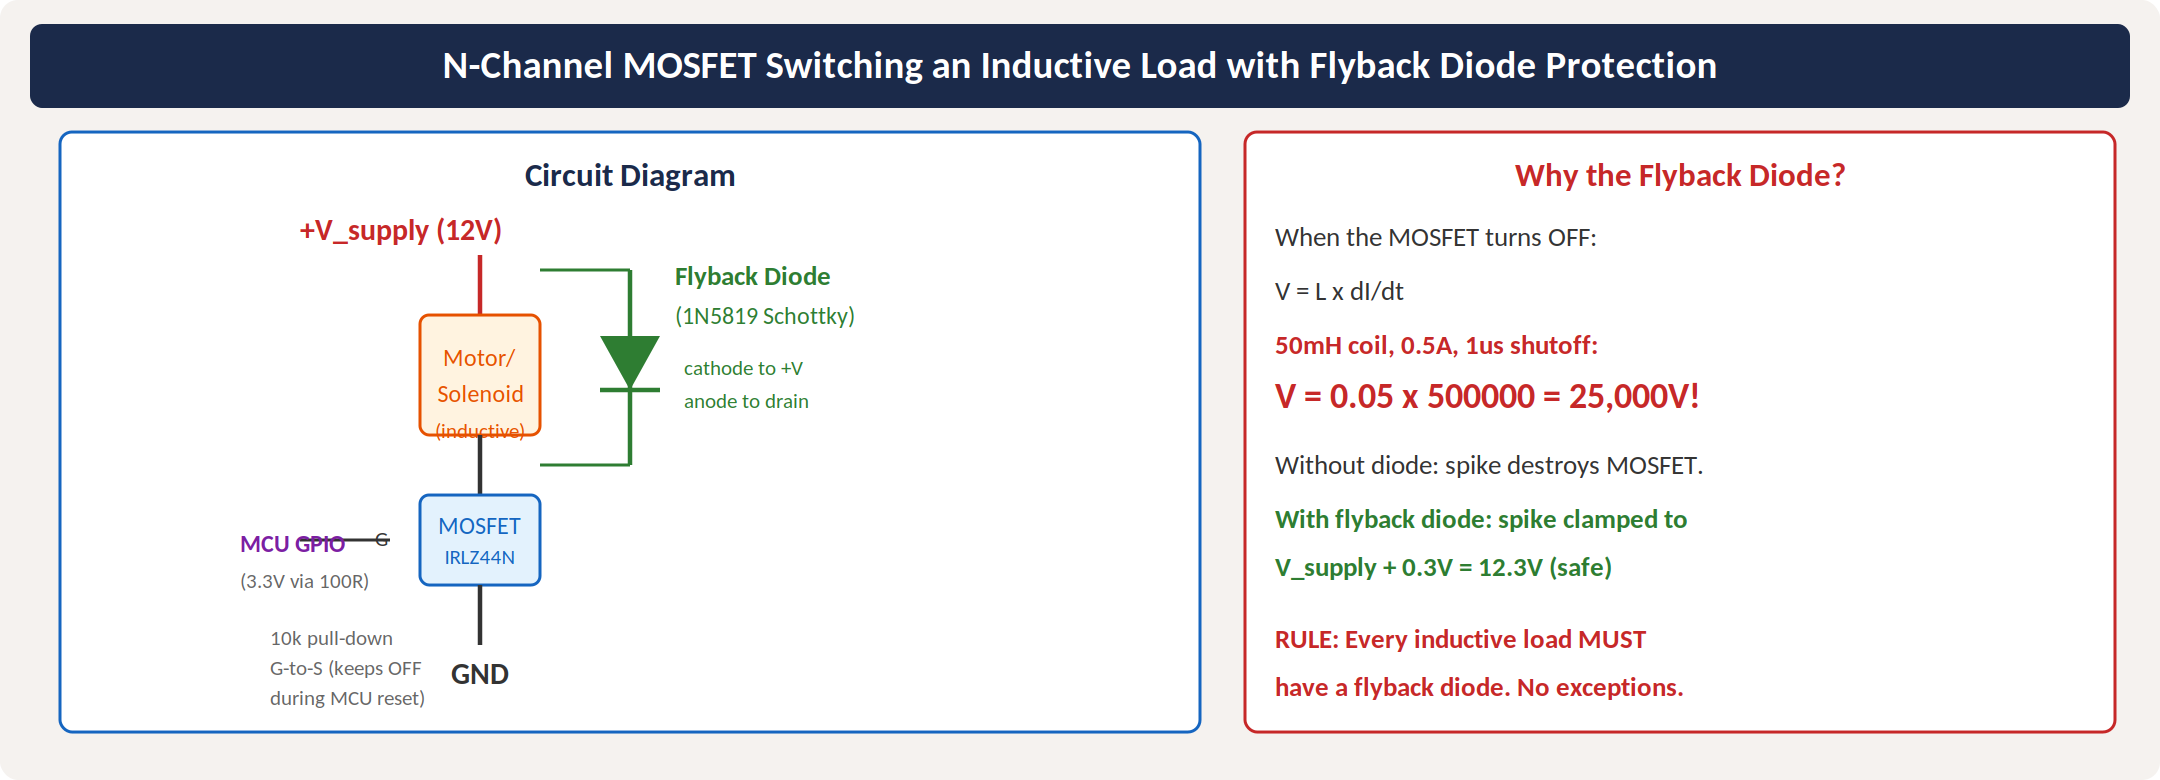
\includegraphics[width=\textwidth]{fig_mosfet_flyback.png}
\caption{N-channel MOSFET switching an inductive load with flyback diode protection. Without the diode, the back-EMF spike from a 50\,mH coil can reach 25,000\,V. The Schottky diode clamps it to $V_{\text{supply}} + 0.3$\,V.}
\label{fig:mosfet_flyback}
\end{figure}

\section{Relays}
An electromechanical switch operated by a coil. The coil is driven by a transistor or MOSFET; the contacts switch the load. \textbf{Advantages}: complete galvanic isolation between control and load, handles AC or DC, very low on-resistance. \textbf{Disadvantages}: slow (5--20\,ms switching), mechanical wear (rated for $10^5$--$10^6$ cycles), audible click, generates EMI from contact arcing.

\subsection{Solid-State Relays (SSR)}
Use a semiconductor (MOSFET or TRIAC) instead of mechanical contacts. No moving parts, no arcing, no audible noise, faster switching ($<$1\,ms), longer lifetime ($>10^8$ cycles). More expensive and have higher on-state voltage drop (generating more heat).

\section{H-Bridge for Motor Direction Control}
An H-bridge uses four switches (MOSFETs or BJTs) arranged so the motor can be driven in both directions. Two switches close at a time (diagonal pairs). PWM on one pair controls speed; switching pairs reverses direction. Common ICs: L298N, BTS7960, DRV8871. Always include flyback protection.


\section{Pulse Width Modulation (PWM) for Power Control}
PWM controls the average power delivered to a load by rapidly switching it on and off. The \textbf{duty cycle} ($D$) determines the fraction of time the load is powered:
\begin{equation}
V_{\text{avg}} = D \times V_{\text{supply}}, \qquad P_{\text{avg}} = D \times P_{\text{max}}
\end{equation}
For a heater or lamp: average power is proportional to duty cycle. For a DC motor: average voltage (and thus speed) is proportional to duty cycle; the motor's mechanical inertia smooths the pulsed current into quasi-continuous rotation.

\textbf{PWM frequency selection}: high enough that the load integrates the pulses (no flicker in lamps, no audible buzz in motors). Typical: 1--25\,kHz for motors, 100\,Hz--1\,kHz for heaters. Too high: increased switching losses in the MOSFET.

\section{Optocouplers and Galvanic Isolation}
An optocoupler transmits a signal across an electrical isolation barrier using light (LED $\to$ phototransistor inside a single package). Provides complete galvanic isolation (typically 3--5\,kV) between the control circuit (MCU) and the power circuit (high-voltage load).

Use optocouplers when: (1) switching AC mains (120/240\,VAC), (2) the power ground and signal ground must be kept separate for safety, or (3) ground loops between the controller and the load circuit must be eliminated.

\begin{examplebox}[ThermoRig: Heater Control with SSR and PWM]
The ThermoRig drives a 120\,VAC, 500\,W cartridge heater through a solid-state relay (SSR, Crydom D2425). The SSR's control input requires 3--32\,VDC at 10\,mA. The ESP32's 3.3\,V GPIO drives the SSR directly (3.3\,V is within the 3--32\,V control range; current draw is 10\,mA, within GPIO limits).

PWM at 1\,Hz (slow PWM or ``time-proportional control''): the PID controller outputs a duty cycle (0--100\%). Each second, the heater is ON for $D \times 1$\,s and OFF for $(1-D) \times 1$\,s. This slow switching extends SSR life and avoids EMI from fast switching of AC loads. The thermal mass of the metal block smooths the pulsed heating into a quasi-continuous temperature rise.
\end{examplebox}


\section{Why High-Power Switching Matters}
Sensors and signal conditioning operate at milliampere levels. Actuators (motors, heaters, solenoids, valves) require amperes. The MCU's GPIO pins cannot drive these loads directly; they provide at most 10--20\,mA at 3.3\,V. A power switching device acts as a gate between the low-power control signal and the high-power load, controlled by the MCU but powered by a separate supply.

\section{MOSFET as a Switch}
The N-channel enhancement MOSFET is the most common switching device in student projects. When gate voltage exceeds the threshold ($V_{GS(th)}$, typically 1--4\,V), the MOSFET conducts between drain and source. When gate is low, it is an open circuit.

Key parameters: \textbf{$V_{GS(th)}$}: must be below the MCU's GPIO voltage. For 3.3\,V MCUs, use logic-level MOSFETs ($V_{GS(th)} < 2.5$\,V; e.g., IRLZ44N, IRL540N). Standard MOSFETs ($V_{GS(th)} \approx 4$\,V) will not fully turn on. \textbf{$R_{DS(on)}$}: drain-source resistance when on. Lower is better; dissipates $P = I^2 \times R_{DS(on)}$ as heat. The IRLZ44N has $R_{DS(on)} = 0.022\,\Omega$ at $V_{GS} = 5$\,V. \textbf{$V_{DS(max)}$}: maximum drain-source voltage when off. Must exceed supply voltage with margin. \textbf{$I_D(max)$}: maximum continuous drain current.

\subsection{Gate Drive Circuit}
The MCU GPIO connects to the MOSFET gate through a series resistor (100--330\,$\Omega$) that limits gate charge current. A pull-down resistor (10\,k$\Omega$) from gate to source ensures the MOSFET stays OFF during MCU reset or high-impedance states. For faster switching, a dedicated gate driver IC can be used.

\section{BJT as a Switch}
Bipolar Junction Transistors (NPN type: TIP120, 2N2222) are also used for switching. The base current controls the collector current: $I_C = \beta \cdot I_B$ where $\beta$ (current gain) is typically 50--200. For saturation (fully on), provide $I_B \geq I_C / \beta_{\min}$ with some margin. A base resistor limits current: $R_B = (V_{GPIO} - V_{BE})/I_B$ where $V_{BE} \approx 0.7$\,V.

MOSFETs are generally preferred for student projects because they require no continuous base current (reducing MCU power) and have lower on-state losses. BJTs are useful for very low-cost applications and Darlington configurations (TIP120) that provide extremely high current gain ($\beta > 1000$).

\section{Inductive Load Protection}
Motors, solenoids, and relays contain inductors. When current through an inductor is suddenly interrupted (MOSFET turns off), the inductor's stored energy ($E = \frac{1}{2}LI^2$) generates a voltage spike:
\begin{equation}
V = L \frac{dI}{dt}
\end{equation}
For a 50\,mH coil carrying 0.5\,A interrupted in 1\,$\mu$s: $V = 0.05 \times 500{,}000 = 25{,}000$\,V. This spike destroys the MOSFET, the MCU, and potentially the DAQ.

A \textbf{flyback diode} (Schottky type: 1N5819) placed across the inductive load (cathode to positive supply, anode to drain) clamps the spike to $V_{\text{supply}} + V_{\text{diode}} \approx V_{\text{supply}} + 0.3$\,V. This is safe. Every inductive load must have a flyback diode. No exceptions.

\section{Relay and SSR Switching}
\textbf{Electromechanical relays}: a coil creates a magnetic field that physically moves a switch contact. Advantages: complete galvanic isolation between control and load, can switch AC or DC, very high off-resistance. Disadvantages: slow (5--20\,ms), limited cycle life (100k--1M operations), generates EMI at contact bounce. The relay coil is itself an inductive load; drive it through a MOSFET or BJT with a flyback diode.

\textbf{Solid-State Relays (SSR)}: semiconductor switches (triacs for AC, MOSFETs for DC) with optical isolation between control and load. Advantages: fast (microseconds), no contact bounce, unlimited cycle life, silent. Disadvantages: some leakage current when off, voltage drop when on (1--2\,V for triacs), requires heat sinking at high currents.

\section{PWM for Proportional Control}
Pulse-Width Modulation (PWM) rapidly switches the load on and off at a fixed frequency, with the ratio of on-time to total period (the \textbf{duty cycle}) controlling the average power delivered. At 50\% duty cycle, the load receives 50\% of the maximum power.

PWM frequency selection: for DC motors, 1--25\,kHz (above audible range to avoid whine). For heaters with SSRs, 0.5--2\,Hz (slow PWM or time-proportional control, matched to the thermal time constant). For LEDs, $>$100\,Hz (above flicker perception).

\section{H-Bridge for Bidirectional Motor Control}
A full H-bridge uses four switching devices (MOSFETs or integrated H-bridge ICs like L298N, DRV8871) arranged so that current can flow through the motor in either direction. By controlling which diagonal pair conducts, the motor spins forward or reverse. PWM on the enable input controls speed. Integrated H-bridge modules include flyback diodes, current sensing, and thermal protection.

\begin{warningbox}[Shoot-Through Protection]
In an H-bridge, if both the high-side and low-side switches in the same leg turn on simultaneously, a short circuit (``shoot-through'') occurs, drawing massive current and potentially destroying the switches. Integrated H-bridge ICs include dead-time protection; if building a discrete H-bridge, add hardware dead-time between complementary gate signals.
\end{warningbox}

\section{Optocoupler Isolation}
When the control circuit (MCU, DAQ) must be electrically isolated from the power circuit (high voltage, noisy motors), an \textbf{optocoupler} provides the link. An LED on the control side illuminates a phototransistor on the power side, transferring the signal across a galvanic barrier. Typical isolation: 2.5--5\,kV. This protects the MCU and DAQ from power-side faults, ground loops, and high-voltage transients.


\section{Relay Selection Guide}
When choosing between electromechanical relays and SSRs:

\textbf{Use electromechanical when}: switching AC mains (the relay's galvanic isolation provides safety), switching infrequently ($<$1 time/second), cost is critical, or the contact resistance must be extremely low ($<$50\,m$\Omega$ for power relays).

\textbf{Use SSR when}: fast switching is needed ($>$1\,Hz), the application requires millions of cycles (heating control, dimming), bounce-free switching is required (digital signal routing), or the system must be silent (laboratory, medical).

\section{Level Shifting}
When the MCU operates at 3.3\,V but the MOSFET gate driver, relay coil, or SSR control requires 5\,V or 12\,V, a level shifter is needed. Simple solutions: (1) NPN transistor with pull-up to the higher voltage (inverts the logic). (2) Dedicated level-shifter IC (TXB0104 for bidirectional, SN74LVC1T45 for unidirectional). (3) Logic-level MOSFET (BSS138) used as a level translator.

\section{Current Sensing}
Measuring the current through a load enables overcurrent protection, power monitoring, and closed-loop current control. Methods: (1) Shunt resistor: insert a small precision resistor ($0.01$--$1\,\Omega$) in series with the load. Measure the voltage drop: $V = I \cdot R_{\text{shunt}}$. Low-side placement (between load and ground) is simplest but shifts the ground reference. High-side placement (between supply and load) preserves the ground but requires a differential amplifier or dedicated high-side current sense IC (INA219, ACS712). (2) Hall-effect sensor: non-contact measurement. No insertion loss. Measures DC and AC. Lower accuracy than shunt but provides galvanic isolation.

\section{Thermal Management}
Power devices dissipate heat ($P = I^2 R_{DS(on)}$ for MOSFETs, $P = V_{CE(sat)} \times I_C$ for BJTs, $P = I^2 R_{\text{contact}}$ for relays). If the junction temperature exceeds the maximum rating ($T_{j,\max}$, typically 150--175\,\degC{} for silicon), the device fails. The thermal path from junction to ambient has a thermal resistance $R_{\theta,JA}$ (\degC{}/W): $T_j = T_{\text{ambient}} + P \times R_{\theta,JA}$. If $T_j$ exceeds limits, add a heatsink to reduce $R_{\theta,JA}$.
\section{Power Budget and Wire Sizing}
Before selecting any switching device, compute the power budget: total current, voltage, and power for each load. Size the wiring accordingly using the American Wire Gauge (AWG) table.

For DC loads: $I = P/V$. A 200\,W heater at 12\,V draws $200/12 = 16.7$\,A. At this current, use 12\,AWG wire minimum (20\,A rating), with appropriately rated connectors and fuses.

\textbf{Voltage drop in wiring}: $V_{\text{drop}} = I \times R_{\text{wire}}$. For 3\,m of 14\,AWG copper ($R = 8.28\,\text{m}\Omega/\text{m}$): $V_{\text{drop}} = 16.7 \times 2 \times 3 \times 0.00828 = 0.83$\,V. This is 7\% of the 12\,V supply, significant enough to affect heater power. Use heavier wire or higher supply voltage.

\textbf{Fuse selection}: size the fuse at 125\% of the normal operating current. For 16.7\,A: use a 20\,A slow-blow fuse. Slow-blow tolerates motor inrush current ($5$--$10\times$ normal for the first 0.1--1\,s); fast-blow fuses trip on inrush.

\section{Solid-State Relay (SSR) Detailed Design}
For AC loads (heaters, lamps, fans powered from mains): the SSR is the standard switching element. It uses a triac (bidirectional thyristor) that turns on when triggered and stays on until the AC current crosses zero.

\textbf{Zero-cross SSR}: triggers only at the next AC zero crossing after the control input is asserted. This prevents inrush current spikes and EMI from mid-cycle switching. Standard for resistive loads (heaters, incandescent lamps).

\textbf{Random-fire SSR}: triggers immediately, regardless of the AC phase. Necessary for phase-angle control (dimming, speed control) but generates significant EMI. Requires an EMI filter.

\textbf{Snubber circuit}: an RC network ($100\,\Omega$ + $0.1\,\mu$F) across the SSR output suppresses voltage transients from inductive loads and prevents false triggering from $dV/dt$ across the triac.

\textbf{Heat sinking}: SSRs have $1$--$1.6$\,V forward drop. At 10\,A: $P = 16$\,W dissipation. Without a heatsink, the SSR overheats and fails. Mount the SSR on an aluminum heatsink with thermal compound; size the heatsink for $R_{\theta} < (T_{\max} - T_{\text{ambient}})/P$.

\section{Motor Control Fundamentals}
\textbf{DC motor speed control}: PWM duty cycle controls average voltage: $V_{\text{avg}} = D \times V_{\text{supply}}$. Speed is approximately proportional to voltage (for unloaded motors). Under load, speed drops due to armature resistance and back-EMF. Closed-loop speed control (tachometer feedback) compensates.

\textbf{Brushless DC (BLDC) motor control}: requires electronic commutation (switching the correct phase winding at the right time). Use a dedicated BLDC driver IC (e.g., DRV8313) or an ESC (Electronic Speed Controller) module. Not practical to implement from discrete components in MEGN~300.

\textbf{Stepper motor control}: moves in discrete angular steps (1.8\degC{}/step typical for a 200-step/revolution motor). Driven by a stepper driver IC (A4988, DRV8825) that converts step and direction signals into the correct coil energization sequence. Interface to MCU: one GPIO for step pulse, one for direction, one for enable.

\section{Protection Circuits}
\textbf{Overcurrent protection}: a fuse or resettable polyfuse in series with the load. For electronic protection: measure current through a shunt resistor and compare to a threshold; if exceeded, disable the MOSFET gate via a comparator circuit. Response time: $<$1\,ms for electronic, 10--100\,ms for fuses.

\textbf{Overvoltage protection}: a TVS (Transient Voltage Suppressor) diode across the power bus clamps voltage spikes from inductive switching, ESD, or supply transients. Select a TVS with standoff voltage above the normal supply and clamping voltage below the maximum rating of the MOSFET and load.

\textbf{Reverse polarity protection}: a MOSFET in the ground return (body diode blocks reverse current) or a series Schottky diode (simple but has 0.3\,V drop). The MOSFET method has negligible voltage drop and is preferred for high-current systems.
\section{EMI from Power Switching}
Every time a MOSFET or SSR switches, it generates electromagnetic interference. The fast voltage transitions ($dV/dt = 100$--$1000$\,V/$\mu$s) and current transitions ($dI/dt = 1$--$100$\,A/$\mu$s) create broadband noise that propagates through power wiring (conducted EMI) and radiates from current loops (radiated EMI). This noise can corrupt analog sensor measurements on the same board or through shared power supplies.

\textbf{Mitigation strategies}: (1) keep power switching traces physically separated from analog signal traces (at least 2\,cm on a PCB, 10\,cm on a protoboard), (2) use a ground plane that separates the power and analog ground return paths, (3) add snubber circuits (RC across the switch) to slow the transitions and reduce $dV/dt$, (4) use gate resistors on MOSFETs to limit $dI/dt$ during turn-on, (5) decouple the analog power supply with LC filters to prevent conducted noise.

\section{Inrush Current Management}
Motors, incandescent lamps, and capacitive loads draw much higher current at turn-on than during steady-state operation:

\textbf{DC motors}: inrush current $= V_{\text{supply}} / R_{\text{armature}}$, typically $5$--$10\times$ the running current. A motor that runs at 2\,A may draw 15\,A at startup. The MOSFET, wiring, and fuse must handle this inrush without tripping or failing.

\textbf{Incandescent lamps}: cold filament resistance is $\sim$$1/10$ of hot resistance. A 100\,W lamp (0.83\,A at 120\,V running) draws $\sim$8\,A at turn-on for the first 100\,ms.

\textbf{Capacitive loads}: charging a capacitor bank produces a current spike $I = V/R_{\text{wire}}$, limited only by the wiring resistance. A 1000\,$\mu$F capacitor charged through 0.1\,$\Omega$ of wiring from 12\,V: peak current $= 120$\,A for a few microseconds. This can weld relay contacts or blow fuses.

\textbf{Solutions}: soft-start circuits (ramp the PWM duty cycle from 0 to target over 0.5--2\,s), NTC inrush limiters (thermistors that have high resistance when cold and low resistance when hot), pre-charge resistors (switched out after initial charging), and current-limiting gate drivers.

\section{Safety Considerations for High-Power Circuits}
\textbf{Stored energy}: capacitors store energy $E = \frac{1}{2}CV^2$. A 1000\,$\mu$F capacitor at 400\,V stores 80\,J, enough to cause serious injury. Capacitors in motor drives and power supplies retain lethal charge for minutes after power-off. Always verify discharge before touching.

\textbf{Arc flash}: at voltages above 48\,V DC or 30\,V AC, an arc can sustain across a small gap (broken wire, relay contact). Arc flash releases intense heat and UV radiation. Use appropriate PPE (safety glasses minimum) when working with circuits above these thresholds.

\textbf{Grounding and isolation}: all exposed metal enclosures must be grounded (connected to the safety ground conductor) to prevent electric shock if an internal fault energizes the enclosure. Use fuses or circuit breakers sized for the wiring, not just the load, to prevent fire from a short circuit.

\textbf{MEGN~300 safety rule}: circuits operating above 48\,V DC or connected to AC mains must be reviewed by the instructor before energizing. All high-current circuits ($> 5$\,A) must include a fuse within 15\,cm of the power source.
\section{Motor Selection for MEGN 300 Projects}
\textbf{DC brushed motors}: simple (two wires), speed proportional to voltage, reversible by polarity swap, easily controlled by PWM through a single MOSFET (one direction) or H-bridge (both directions). Drawback: brushes wear, generate EMI, and limit speed. Use for: pumps, fans, linear actuators, and simple drive systems.

\textbf{DC brushless (BLDC)}: higher efficiency, longer life, less EMI. Require electronic commutation (ESC or motor driver IC). Cannot be driven by a simple MOSFET. Use for: high-performance drives, drones, precision positioning.

\textbf{Stepper motors}: precise angular positioning without feedback (open-loop). 200 steps/revolution (1.8\degC{}/step) standard. Driven by dedicated stepper driver (A4988, DRV8825). Low cost, high torque at low speed, easy position control. Use for: 3D printers, CNC motion, laboratory positioning stages.

\textbf{Servo motors}: DC motor + encoder + PID controller in a closed-loop package. Precise position and speed control. Standard hobby servos accept a PWM signal (1--2\,ms pulse width at 50\,Hz). Industrial servos use CAN, EtherCAT, or analog $\pm$10\,V command. Use for: robotic joints, valve actuators, camera gimbals.

\textbf{Selection criteria}: (1) required torque and speed (check the motor's torque-speed curve), (2) voltage and current (must match available power supply and switching devices), (3) size and weight, (4) control complexity (brushed DC is simplest; BLDC requires a driver), (5) lifetime requirement (brushed: 1000--5000 hours; brushless: 20{,}000+ hours).

\section{Power Electronics Thermal Design}
Every switching device dissipates power as heat. The thermal design must ensure the junction temperature stays below the maximum rating:

\begin{equation}
T_j = T_{\text{ambient}} + P_{\text{diss}} \times (R_{\theta,JC} + R_{\theta,CS} + R_{\theta,SA})
\end{equation}
where $R_{\theta,JC}$ is junction-to-case (from datasheet), $R_{\theta,CS}$ is case-to-sink (depends on thermal interface: $\sim$0.5\,\degC{}/W with thermal paste, $\sim$2\,\degC{}/W with bare contact), and $R_{\theta,SA}$ is sink-to-ambient (from heatsink datasheet).

Example: IRLZ44N MOSFET ($R_{\theta,JC} = 1.5$\,\degC{}/W), thermal paste ($R_{\theta,CS} = 0.5$), switching 5\,A with $R_{DS(on)} = 0.022\,\Omega$: $P = 5^2 \times 0.022 = 0.55$\,W. Without heatsink ($R_{\theta,JA} = 62$\,\degC{}/W): $T_j = 25 + 0.55 \times 62 = 59$\,\degC{} (safe, $< 175$\,\degC{} limit). At 20\,A: $P = 8.8$\,W, $T_j = 25 + 8.8 \times 62 = 571$\,\degC{} (destroyed!). Need a heatsink: $R_{\theta,SA} < (175-25)/8.8 - 2 = 15$\,\degC{}/W.
\section{DC-DC Converters: Buck and Boost Regulators}

The switching transistors and PWM concepts covered earlier in this chapter have a direct application beyond motor control: DC-DC power conversion. Most instrumentation systems require multiple voltage rails (3.3\,V for the MCU, 5\,V for sensors, 12\,V or 24\,V for actuators) from a single source. Linear regulators (LDOs) can step voltage down, but they dissipate the voltage difference as heat: a 12\,V to 3.3\,V LDO wastes 72\% of the input power. Switching regulators solve this by rapidly chopping the input voltage and using an inductor to transfer energy efficiently, achieving 85--95\% efficiency.

\subsection{Buck Converter (Step-Down)}
A buck converter produces an output voltage lower than the input. The core circuit has four elements: a switching MOSFET, a diode (or synchronous MOSFET), an inductor, and an output capacitor. The MOSFET switches at 100\,kHz--2\,MHz with a duty cycle $D$. During the ON phase, current flows through the MOSFET and inductor to the load, storing energy in the inductor's magnetic field. During the OFF phase, the inductor's stored energy drives current through the diode to the load, maintaining continuous current flow.

The output voltage is controlled by the duty cycle:
\begin{equation}
V_{\text{out}} = D \times V_{\text{in}}, \qquad D = \frac{V_{\text{out}}}{V_{\text{in}}}
\end{equation}

For a 12\,V to 3.3\,V conversion: $D = 3.3/12 = 0.275$ (27.5\% duty cycle). The MOSFET is ON for 27.5\% of each switching period and OFF for 72.5\%. Efficiency is typically 85--95\%, meaning only 5--15\% of the input power is wasted as heat, compared to 72\% for an LDO doing the same conversion.

\textbf{Common buck converter ICs for student projects}: LM2596 (3\,A, adjustable, through-hole friendly), MP1584 (3\,A, compact module), LM3671 (600\,mA, ultra-compact for battery applications).

\begin{tipbox}[When to Use a Buck vs. an LDO]
Use an LDO when: (1) the voltage drop is small ($V_{\text{in}} - V_{\text{out}} < 2$\,V), (2) current is under 500\,mA, (3) you need very low output noise (analog sensor circuits, precision ADCs), or (4) simplicity matters (an LDO needs only two capacitors). Use a buck converter when: (1) the voltage drop is large ($>$2\,V), (2) current exceeds 500\,mA, (3) efficiency matters (battery-powered systems), or (4) the heat from an LDO would be problematic. Many systems use both: a buck to step 12\,V down to 5\,V efficiently, then an LDO to produce a clean 3.3\,V from that 5\,V rail.
\end{tipbox}

\subsection{Boost Converter (Step-Up)}
A boost converter produces an output voltage higher than the input. The topology reverses the buck: the inductor is on the input side, the MOSFET shorts the inductor to ground during the ON phase (storing energy), and during the OFF phase the inductor's energy adds to the input voltage and charges the output capacitor through the diode.

\begin{equation}
V_{\text{out}} = \frac{V_{\text{in}}}{1 - D}
\end{equation}

For a 3.7\,V lithium cell boosted to 5\,V: $D = 1 - 3.7/5 = 0.26$ (26\% duty cycle). As duty cycle approaches 1.0, the theoretical output approaches infinity, but practical limits (inductor saturation, diode losses, parasitic resistance) restrict useful boost ratios to about 4:1.

\textbf{Applications in MEGN~300}: powering a 5\,V sensor system from a single 3.7\,V lithium cell, generating a 12\,V rail for relay coils from a 5\,V USB supply, and driving LED strings that require higher voltage than the available supply.

\subsection{Buck-Boost Converter}
A buck-boost converter can produce an output voltage either higher or lower than the input. This is essential when the input varies across the output target: a lithium battery ranges from 4.2\,V (fully charged) to 3.0\,V (discharged). If the system needs 3.3\,V, neither a pure buck nor a pure boost works across the full range. A buck-boost handles both conditions seamlessly.

The SEPIC (Single-Ended Primary-Inductor Converter) is a popular buck-boost topology that produces a non-inverted output with good regulation. Common ICs: TPS63000 series (Adjustable, 1.8--5.5\,V output, 96\% peak efficiency).

\subsection{Switching Regulator Noise}
The main disadvantage of all switching regulators is output ripple and electromagnetic interference (EMI). The rapid switching (100\,kHz+) generates noise at the switching frequency and its harmonics. This noise can corrupt sensitive analog measurements.

Mitigation strategies: (1) add an LC output filter (extra inductor + capacitor) after the switching regulator, (2) use an LDO as a post-regulator to clean up the output for analog circuits, (3) keep switching regulator traces physically separated from analog signal traces on the PCB, and (4) use a continuous ground plane under the switching regulator with short, wide power traces. The Master Reference Document PCB Design chapter (Chapter~16) covers layout best practices for switching regulators.

\begin{examplebox}[ThermoRig: Multi-Rail Power Architecture]
The ThermoRig uses a 12\,V wall adapter as its primary source. A buck converter (LM2596 module) steps 12\,V down to 5\,V at up to 2\,A for the sensor power rail (85\% efficient, 0.3\,W waste heat vs. 2.6\,W for an LDO). An LDO (AMS1117-3.3) then produces 3.3\,V from the 5\,V rail for the ESP32 (66\% efficient, but only 300\,mA, so waste heat is 0.5\,W, manageable). The 12\,V rail directly powers the heater SSR control and the cooling fan. Total power architecture: three voltage rails from one input, with the high-current conversion handled by the switching regulator and the noise-sensitive MCU rail cleaned up by the LDO.
\end{examplebox}

\begin{keyconceptbox}[Requirements Mapping: Power Conversion]
``The power supply system shall convert the 12\,VDC input to a regulated 5.0\,V $\pm$ 3\% rail at up to 2\,A continuous.'' ``The 3.3\,V MCU rail shall have output ripple less than 30\,mV peak-to-peak measured at the ESP32 power pins.'' ``The power supply system shall achieve a minimum overall efficiency of 80\% at full rated load.'' ``All switching regulator modules shall include input and output capacitors per the manufacturer's reference design.''
\end{keyconceptbox}

\section{Functional Safety: Fail-Safes and Emergency Stops}
\subsection{What Happens When the Controller Fails?}
Every automation system must answer this question: if the microcontroller crashes, the software enters an infinite loop, the communication link drops, or the power supply glitches, what happens to the actuators?

If the heater stays ON at 100\% power because the MCU froze: the system overheats, potentially causing fire, burns, or property damage. If the motor continues running because the stop command was never sent: the mechanism can drive into a hard stop, destroying gears, bending shafts, or ejecting workpieces.

\textbf{The fundamental principle}: the system must always transition to a safe state when control is lost. The safe state is application-specific: for a heater, safe means OFF. For a vehicle brake, safe means ENGAGED. For an emergency ventilation system, safe means ON. Define the safe state for every actuator in your system during the requirements phase.

\subsection{Fail-Safe Design Patterns}
\textbf{Normally-open (NO) relay/contactor}: the actuator is powered through a relay that is held closed by the controller's ``enable'' signal. If the controller loses power or crashes, the relay opens (spring-return), cutting power to the actuator. This is the Master Control Relay (MCR) pattern and is the standard for industrial safety circuits.

Implementation for MEGN~300: connect the heater or motor power through a relay. The relay coil is driven by a GPIO pin through a MOSFET. The firmware keeps the relay energized during normal operation. If the MCU resets, the GPIO defaults to LOW (output disabled), the MOSFET turns OFF, the relay opens, and the heater is de-energized. The system fails safe without any software action.

\textbf{Watchdog timer}: a hardware timer that must be periodically reset (``kicked'') by the firmware. If the firmware crashes or enters an infinite loop and stops kicking the watchdog, the timer expires and forces a system reset. The ESP32 has a built-in watchdog with configurable timeout (1--60\,s). After reset, the firmware initializes all outputs to the safe state before resuming normal operation.

\textbf{Hardware E-Stop}: a physical emergency stop button (large, red, mushroom-head, per IEC~60947-5-5) that cuts power to all actuators independently of the controller. The E-Stop circuit is wired in series with the MCR and is always hardwired (never software-controlled). Pressing the E-Stop physically opens the relay, regardless of the controller state. The button latches in the pressed position; the operator must deliberately release it (twist to reset) before the system can restart.

\begin{warningbox}[Software Cannot Be the Last Line of Defense]
A software-only safety system is not a safety system. Software crashes, firmware has bugs, and communication links drop. The E-Stop, the MCR, and the watchdog timer are hardware mechanisms that function independently of software. In professional automation (IEC~61508, ISO~13849), the safety function must be implemented in hardware that is separate from and independent of the control system. For MEGN~300 projects: at minimum, include a physical power switch (toggle or E-Stop button) that cuts actuator power independently of the MCU.
\end{warningbox}

\subsection{Safety Integrity Levels (Conceptual)}
The international standard IEC~61508 defines Safety Integrity Levels (SIL 1--4) that quantify the required reliability of safety functions. SIL~1: probability of dangerous failure $< 10^{-1}$ per demand ($<$10\% chance of the safety function failing when needed). SIL~4: $< 10^{-4}$ ($<$0.01\%). Higher SIL requires more rigorous design, redundancy, and testing.

MEGN~300 projects do not require formal SIL assessment, but understanding the concept demonstrates professional awareness. A single E-Stop relay with no redundancy is approximately SIL~1. Adding a second, independent relay (both must be energized for the actuator to operate) approaches SIL~2.

\subsection{Practical Implementation for GreenShield Projects}
Every MEGN~300 project with actuators (heaters, motors, pumps, solenoids) shall include:

(1) A physical power disconnect (switch, button, or E-Stop) that cuts power to all actuators independently of the MCU.

(2) A watchdog timer (ESP32 built-in) that resets the system if firmware hangs for more than 5\,s.

(3) Software current and temperature limits that de-energize actuators if readings exceed safe thresholds ($> 150\%$ of normal operating values).

(4) A ``safe state'' initialization routine that sets all outputs to OFF on startup, before any control logic executes.
\section{Practice Questions}
\begin{enumerate}[leftmargin=1.5em]
\item Your MCU (3.3\,V GPIO, 10\,mA max) must switch a 12\,V, 2\,A DC motor. Design the switching circuit using an N-channel MOSFET. Specify the MOSFET selection criteria and include flyback protection.
\item Explain why you cannot connect a 120\,VAC heater directly to a MOSFET, and describe how you would control it instead.
\item A solenoid draws 500\,mA at 24\,V. The control MOSFET opens in 1\,$\mu$s. If the solenoid inductance is 50\,mH, what voltage spike would occur without a flyback diode?
\end{enumerate}

\subsection{Answers}
\begin{enumerate}[leftmargin=1.5em]
\item Select a logic-level N-channel MOSFET (e.g., IRLZ44N: $V_{th} = 1.0$--$2.0$\,V, $R_{DS(on)} = 0.022\,\Omega$ at $V_{GS} = 4.5$\,V, $I_D = 47$\,A). Connect: drain to motor negative, source to ground, gate to MCU GPIO through a 100\,$\Omega$ resistor (limits gate charge current). Add a 10\,k$\Omega$ pull-down from gate to source (ensures MOSFET stays off when MCU is in reset). Flyback diode: 1N5819 Schottky (40\,V, 1\,A) across motor terminals (cathode to $+$12\,V, anode to drain). Power dissipation: $2^2 \times 0.022 = 0.088$\,W; no heatsink needed.
\item MOSFETs switch DC only (they conduct in one polarity). For 120\,VAC, use: (a) an electromechanical relay with a MOSFET driving the coil, or (b) a solid-state relay (SSR) rated for the voltage and current. The SSR uses a TRIAC internally that handles AC polarity reversal. Ensure the SSR is rated for 120\,VAC and the full heater current with derating.
\item $V = L \times dI/dt = 0.050 \times (0.500/0.000001) = 25{,}000$\,V. This 25\,kV theoretical spike (in practice clamped by parasitic capacitance and eventual breakdown) far exceeds any MOSFET's voltage rating. A flyback diode clamps it to approximately $24 + 0.3 = 24.3$\,V.
\end{enumerate}


% ################################################################
% PART IV: CONTROL SYSTEMS
% ################################################################
\part{Control Systems}

\chapter{Open-Loop Control}

\section{Definition}
In open-loop control, the controller sends a command to the actuator without measuring the output. There is no feedback; the controller has no way to know if the desired outcome was achieved.

\textbf{Example}: a toaster. You set a timer (the command); the heating element runs for that duration regardless of how toasted the bread actually is. If the bread type, thickness, or initial temperature changes, the result changes, but the controller does not adapt.

\section{Characteristics}
\begin{itemize}[leftmargin=1.5em]
\item \textbf{Simple}: no sensor needed on the output; fewer components; lower cost.
\item \textbf{Fast}: no processing delay from feedback.
\item \textbf{No stability issues}: cannot oscillate (no feedback loop to create instability).
\item \textbf{Cannot compensate for disturbances}: if the environment changes (load, temperature, friction), the output drifts from the desired value with no correction.
\item \textbf{Accuracy depends on the model}: the controller must have a perfect model of the plant to achieve the desired output. Any model error becomes output error.
\end{itemize}

\section{Feedforward Control}
A refined form of open-loop control that measures the disturbance (not the output) and adjusts the command proactively. Example: measuring outdoor temperature and preemptively increasing heater power before the room cools down. Feedforward improves performance but still has no feedback on the actual output.

\begin{figure}[htbp]
\centering
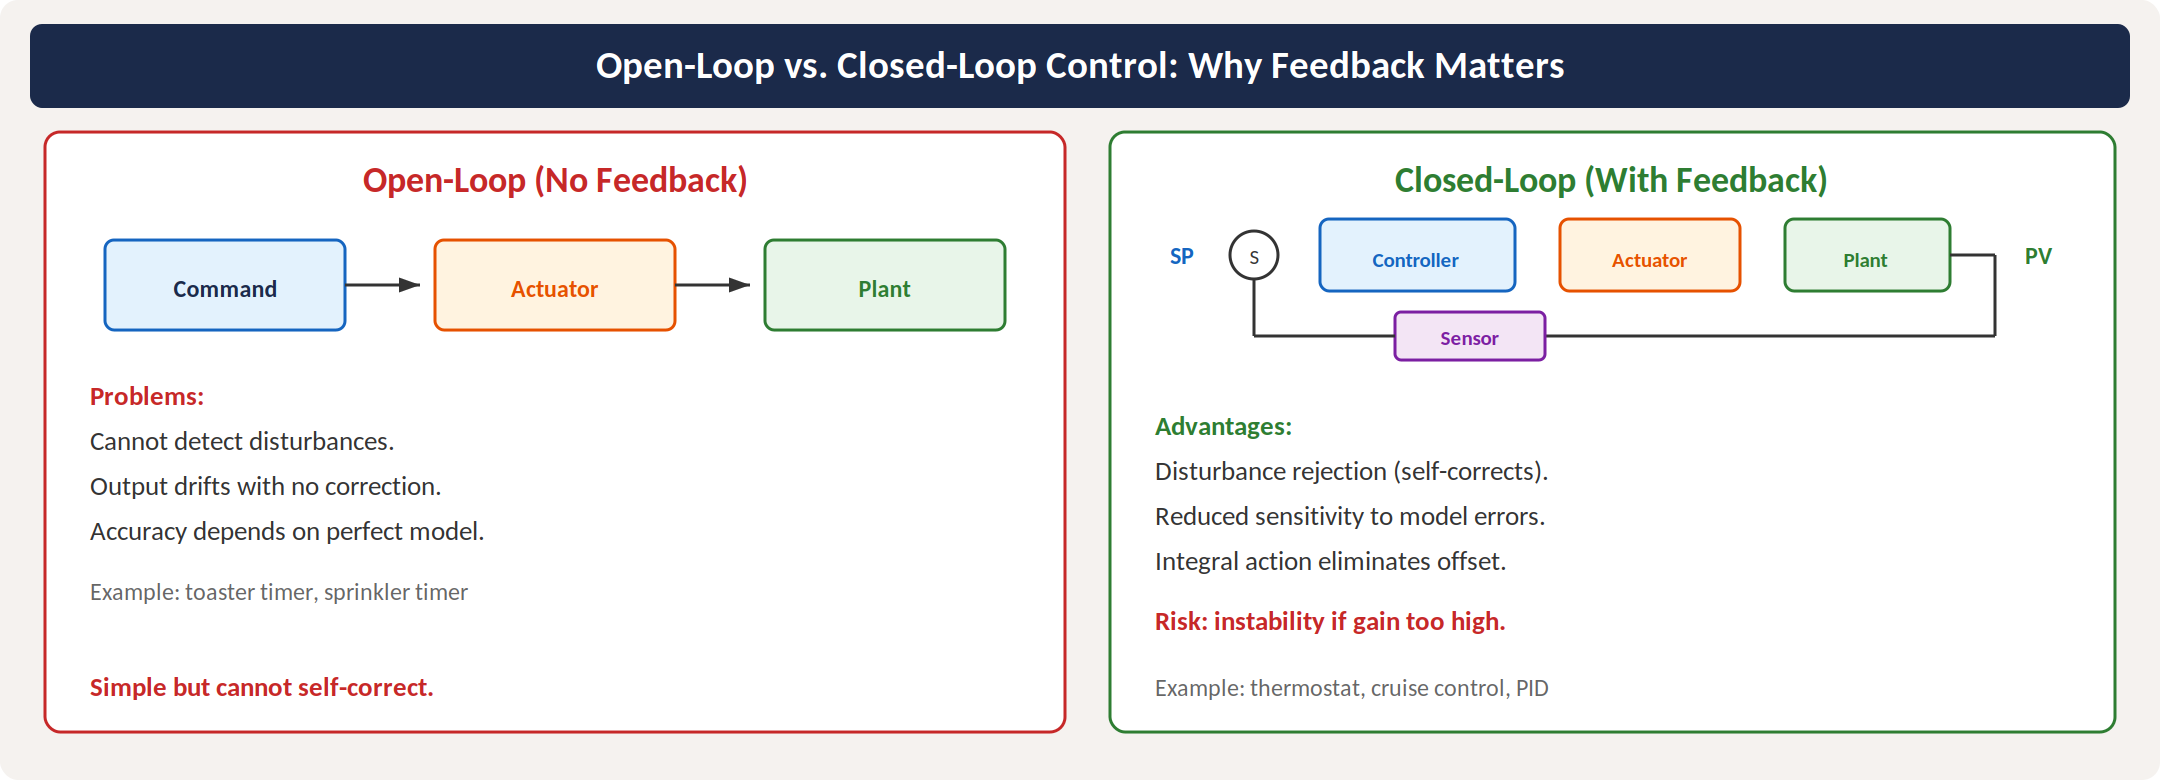
\includegraphics[width=\textwidth]{fig_open_vs_closed.png}
\caption{Open-loop vs.\ closed-loop control. Open-loop is simple but cannot detect or correct disturbances. Closed-loop uses sensor feedback to self-correct, enabling disturbance rejection and zero steady-state error with integral action.}
\label{fig:open_closed}
\end{figure}


\section{Understanding Open-Loop Control}
In open-loop control, the controller sends a command to the actuator based on a model or schedule, with no measurement of the actual output. The system has no way to detect or correct errors. Examples: a toaster timer (runs for a fixed duration regardless of toast darkness), a washing machine cycle timer (runs predetermined durations for each phase), and a sprinkler timer (waters for a set time regardless of soil moisture).

Open-loop works when the relationship between input and output is well-characterized and disturbances are small or predictable. It is simple, cheap, and inherently stable (no feedback means no oscillation risk). However, it fails when disturbances are significant, when the plant model is inaccurate, or when precise output control is required.

\section{Feedforward Control}
Feedforward is an enhanced form of open-loop that measures the disturbance (not the output) and adjusts the control action proactively. Example: measuring outdoor temperature and adjusting the furnace output before the room temperature changes. Feedforward cannot correct for unmeasured disturbances or model errors, but it responds faster than feedback because it does not wait for the output to deviate.

In practice, feedforward is often combined with feedback: the feedforward handles the known, measurable disturbances (fast), while the feedback corrects for everything else (robust). This combined approach is standard in industrial process control.

\section{Limitations of Open-Loop}
\textbf{No disturbance rejection}: any unmodeled influence (load change, supply variation, environmental shift) directly affects the output with no correction.

\textbf{Sensitivity to model errors}: the accuracy of the output depends entirely on the accuracy of the model relating input to output. If the model is wrong, the output is wrong, and the system has no way to know.

\textbf{No steady-state accuracy guarantee}: drift, aging, and environmental changes cause the output to wander from the desired value over time.

\section{When Open-Loop Is Appropriate}
Despite its limitations, open-loop control is the right choice when: the cost of feedback sensors is prohibitive, the plant behavior is highly predictable and disturbances are negligible, the required accuracy is coarse (e.g., a traffic light timer), or when stability concerns make feedback dangerous (some chemical processes).


\section{Feedforward Control}
Feedforward measures the disturbance (not the output) and adjusts the control action proactively. Example: measuring outdoor temperature and adjusting furnace output before room temperature changes. Advantages: responds faster than feedback (does not wait for error). Limitations: cannot correct for unmeasured disturbances or model errors. In practice, feedforward is combined with feedback for optimal performance.

\section{Calibration Tables as Open-Loop Control}
A common form of open-loop control in instrumentation is the calibration table or lookup table. Rather than modeling the sensor's response analytically, the controller stores measured input-output pairs and interpolates between them. Example: a thermocouple's voltage-to-temperature relationship stored as a 100-entry table, with linear interpolation between entries. This is ``open-loop'' because it relies on the accuracy of the stored calibration data, with no feedback to verify the output.

\section{State Machines as Open-Loop Controllers}
Many laboratory instruments use state-machine controllers: a sequence of states (initialize, preheat, measure, cool down, report) with timed transitions. Each state commands specific actuator settings. The sequence runs to completion regardless of the process outcome. This is open-loop because the controller follows a predetermined script. Adding sensor checks that branch to error-handling states converts it to a hybrid open/closed-loop system.

\section{When Open-Loop Fails}
Example: you calibrate a heater to deliver 80\,\degC{} at 50\% power. Initially, it works. Three months later, the ambient temperature drops from 22\,\degC{} to 10\,\degC{}, and the heater only reaches 68\,\degC{}. The open-loop controller has no way to detect or correct this. A closed-loop controller would measure the 68\,\degC{} output, compute a 12\,\degC{} error, and increase power automatically.
\section{Mathematical Model of Open-Loop Systems}
In open-loop control, the output $Y(s) = G_p(s) \cdot G_a(s) \cdot U(s) + G_d(s) \cdot D(s)$ where $G_p$ is the plant transfer function, $G_a$ is the actuator, $U$ is the command, $G_d$ is the disturbance transfer function, and $D$ is the disturbance. The output depends on both the command and the disturbance, with no mechanism to separate or correct for the disturbance contribution.

For a linear system with known plant model: $U = G_p^{-1} \cdot Y_{\text{desired}}$ (invert the plant model to compute the required command). This works perfectly if the model is exact and no disturbances exist. In practice, model uncertainty of $\pm$10\% produces $\pm$10\% output error, and disturbances add directly to the output.

\section{Examples of Open-Loop Systems in Engineering}
\textbf{CNC machine tool positioning}: the stepper motor receives a commanded number of steps, and the controller assumes the table moves exactly that distance. No position feedback (in basic systems). If the motor skips a step (due to excessive load or acceleration), the error accumulates permanently. High-end CNC machines add encoder feedback (closed-loop).

\textbf{Irrigation timer}: opens the water valve for a programmed duration. Does not measure soil moisture, rainfall, or evapotranspiration. Wastes water during rain and under-waters during heat waves. Smart irrigation systems add soil moisture sensors (closed-loop).

\textbf{Inkjet printer head positioning}: the carriage motor moves based on commanded pulses. Open-loop in the fast-scan direction (relying on motor accuracy). Closed-loop in the slow-scan direction (optical encoder on the paper feed roller).

\textbf{Drug delivery infusion pump}: delivers a programmed flow rate based on motor speed. Open-loop with respect to actual drug concentration in the patient's blood. Closed-loop drug delivery (measuring blood concentration and adjusting the rate) exists in research but is rare clinically due to sensor limitations.

\section{Quantifying Open-Loop Performance}
The performance of an open-loop system depends entirely on: (1) model accuracy: the relationship between command and output must be precisely characterized, (2) disturbance magnitude: smaller disturbances produce smaller output errors, (3) component repeatability: the actuator must produce the same output for the same command every time, (4) environmental stability: temperature, humidity, and other conditions must remain within the range over which the model is valid.

For the ThermoRig heater in open-loop mode: commanding 50\% PWM duty cycle produces approximately 65\,\degC{} at ambient 22\,\degC{}. If the ambient temperature drops to 15\,\degC{}, the steady-state temperature drops to approximately 58\,\degC{} (a 7\,\degC{} error). If the supply voltage drops from 12\,V to 11\,V (8\% drop), the power drops by 16\% (power $\propto V^2$), and the temperature drops further. The open-loop system cannot detect or correct any of these deviations.

\section{Feedforward Design Procedure}
For measured disturbance $d$ with known effect on the output: (1) measure $d$ with a sensor. (2) Compute the required compensation: $\Delta u = -G_d(s)/G_p(s) \cdot d$ (the feedforward transfer function). (3) Add $\Delta u$ to the nominal command: $u = u_{\text{nominal}} + \Delta u$.

Example: the ThermoRig measures ambient temperature $T_{\text{amb}}$ with a second thermocouple. The thermal model predicts that a 1\,\degC{} drop in ambient requires 0.8\% more heater power to maintain the setpoint. The feedforward controller adds $0.8\% \times (T_{\text{amb,nominal}} - T_{\text{amb,measured}})$ to the duty cycle. This compensates for ambient temperature changes without waiting for the output temperature to deviate.

Combined feedforward + feedback: the feedforward handles the measured, predictable disturbance (ambient temperature) immediately, while the feedback (PID controller) corrects for unmeasured disturbances (supply voltage variation, heater degradation, model error). The result is faster disturbance rejection than feedback alone and more robust than feedforward alone.

\section{Open-Loop Stability}
Open-loop systems are always stable (in the BIBO sense) as long as the plant itself is stable. There is no feedback to create oscillation. This is a significant advantage in applications where stability is critical and the accuracy requirement is relaxed (e.g., a simple fan speed controller where $\pm$10\% speed error is acceptable but oscillation would be unacceptable).

However, plants with integrators (e.g., liquid level in a tank with inflow but no outflow) are inherently unstable in open-loop: the level rises without bound unless the inflow is precisely balanced with the outflow. Such systems require closed-loop control.
\section{Lookup Tables and Interpolation in Open-Loop Control}
Many open-loop systems use precomputed lookup tables rather than mathematical models. For the ThermoRig in open-loop mode: measure the steady-state temperature at 10 duty cycle values (0\%, 10\%, 20\%, \ldots, 100\%) and store the results in a table. To achieve a desired temperature, look up the nearest duty cycle and interpolate linearly between table entries.

Limitations: (1) the table is valid only at the ambient temperature at which it was measured, (2) any change in heater resistance (aging), supply voltage, or thermal coupling invalidates the table, (3) the temperature can only be set to discrete values (the table resolution), (4) transient behavior is uncontrolled (the system takes whatever path it takes to reach the new steady state).

\section{State Machine Controllers}
Many laboratory instruments use state-machine (sequential) controllers. A typical sequence for the ThermoRig: INITIALIZE (set outputs to safe state) $\to$ PREHEAT (ramp heater to approximate temperature) $\to$ STABILIZE (wait 5 minutes for thermal equilibrium) $\to$ MEASURE (acquire 1000 samples) $\to$ COOL (turn off heater, wait) $\to$ REPORT (compute statistics, save file).

Each state has a fixed duration or a simple exit condition (e.g., ``temperature within 5\,\degC{} of target''). The controller does not optimize performance within each state; it follows the script. This is robust and predictable but inflexible. If the preheat phase does not reach the target (due to a disturbance), the stabilize phase may not produce equilibrium, and the measurement phase produces incorrect data. A closed-loop controller would detect and correct this; the state machine does not.

\section{Combining Open-Loop and Closed-Loop}
Practical systems often combine both approaches. The state machine manages the high-level sequence (start, run, stop, error handling), while closed-loop controllers manage the low-level performance within each state. In the ThermoRig: the state machine sequences the test protocol, while a PID controller maintains the temperature within the STABILIZE and MEASURE states. This is the architecture used in most commercial test equipment.
\section{Characterizing Plant Dynamics in Open Loop}
Before designing a controller (open or closed-loop), you must know how the plant responds. The standard method: apply a step input and record the output.

For the ThermoRig in open-loop: set the heater to 50\% duty cycle (step from 0\%) and record the temperature vs.\ time. The response curve shows: (1) a transport delay $L$ (dead time) before the temperature begins rising (heat propagating from the heater to the thermocouple), (2) an exponential-like rise toward the steady-state temperature, and (3) a final steady-state temperature $T_{ss}$.

From this step response, extract three parameters: the process gain $K_p = (T_{ss} - T_{\text{ambient}}) / (\text{duty cycle change})$, the time constant $\tau$ (time to reach 63.2\% of $T_{ss} - T_{\text{ambient}}$), and the dead time $L$ (time from the step to the first observable temperature rise). For the ThermoRig: $K_p \approx 1.1$\,\degC{}/\%, $\tau \approx 30$\,s, $L \approx 3$\,s.

These three parameters ($K_p$, $\tau$, $L$) define a First-Order Plus Dead Time (FOPDT) model: $G(s) = K_p e^{-Ls} / (1 + \tau s)$, which is the most common plant model used for PID tuning in process control.

\section{Sensitivity Analysis}
How much does the open-loop output change when a parameter varies?

\textbf{Supply voltage}: heater power $P = V^2/R$. A 10\% voltage drop reduces power by 19\% (because $P \propto V^2$). For the ThermoRig: $T_{ss}$ drops by approximately 12\,\degC{} for a 10\% voltage reduction. The open-loop controller does not detect this.

\textbf{Ambient temperature}: every 1\,\degC{} change in ambient shifts the steady-state temperature by approximately 0.9\,\degC{} (because the thermal resistance is nearly constant). A 10\,\degC{} seasonal variation produces a 9\,\degC{} output error.

\textbf{Heater aging}: over thousands of hours, the heater element resistance increases (wire oxidation), reducing power. A 5\% resistance increase reduces power by 5\% and $T_{ss}$ by approximately 3\,\degC{}.

These sensitivity calculations quantify why open-loop control is inadequate when precision matters. A closed-loop controller compensates for all of these disturbances automatically.

\section{Hybrid Architectures in Industrial Practice}
Most real industrial systems use a hierarchy of control:

\textbf{Level 1 (open-loop sequencing)}: a PLC or state machine manages the process sequence (fill tank, heat, hold, cool, drain). This is deterministic and testable.

\textbf{Level 2 (closed-loop regulation)}: PID controllers maintain temperature, pressure, flow, and level within each process step. These respond to disturbances in real time.

\textbf{Level 3 (supervisory optimization)}: a higher-level controller (often model-predictive control, MPC) adjusts the setpoints of the Level~2 controllers to optimize the overall process (minimize energy, maximize throughput, meet quality targets).

Understanding open-loop control as one layer in this hierarchy, rather than as a standalone approach, provides the proper engineering perspective.
\section{Open-Loop Control in Embedded Systems}
Many microcontroller-based systems use open-loop control for non-critical functions while reserving closed-loop for critical ones:

\textbf{Stepper motor positioning}: the MCU commands a specific number of step pulses, and the motor is assumed to move one step per pulse. No position feedback. This works for light loads and moderate speeds but fails under high load (motor skips steps) or high acceleration (motor stalls). Adding an encoder closes the loop and enables step-loss detection and recovery.

\textbf{LED brightness control}: PWM duty cycle sets the average LED current. The brightness is assumed proportional to current (approximately true for most LEDs). No light sensor feedback. Adequate for indicator LEDs and displays; insufficient for precision photometric applications where LED aging, temperature, and manufacturing variation affect the current-to-luminance relationship.

\textbf{Timed dispensing}: a solenoid valve opens for a fixed duration to dispense a volume of liquid. The volume is assumed proportional to time (true if pressure and viscosity are constant). Variations in supply pressure, fluid temperature (viscosity changes), or valve wear produce volume errors. Closed-loop dispensing (measuring the actual volume or weight during dispensing) eliminates these errors.

\section{Feedforward Control: Design and Implementation}
Feedforward control measures a disturbance before it affects the output and applies a preemptive correction. It requires a model of how the disturbance affects the output.

\textbf{Design procedure}: (1) Identify the dominant measurable disturbance. (2) Model its effect on the output: $\Delta y = G_d \cdot d$ where $G_d$ is the disturbance transfer function. (3) Compute the required feedforward correction: $\Delta u_{ff} = -(G_d/G_p) \cdot d$ where $G_p$ is the plant transfer function. (4) Implement: measure $d$ with a sensor, compute $\Delta u_{ff}$, and add it to the nominal control output.

\textbf{Example}: the ThermoRig operates at $T_{\text{sp}} = 80$\,\degC{}. The dominant disturbance is ambient temperature variation. Model: a 1\,\degC{} drop in ambient requires approximately 0.8\% additional heater duty cycle to compensate (determined by measuring the steady-state duty cycle at two ambient temperatures). Feedforward: $\Delta u_{ff} = 0.8\% \times (T_{\text{amb,ref}} - T_{\text{amb,measured}})$. Combined with PID feedback: the feedforward corrects 80\% of the disturbance effect immediately (within one control loop period), while the PID corrects the remaining 20\% (model error, unmeasured disturbances) over the next few time constants.

\section{Model-Based Open-Loop: Inverse Dynamics}
For systems where the plant dynamics are well-characterized, \textbf{inverse dynamics} computes the exact input needed to produce the desired output trajectory. If the plant transfer function is $G_p(s)$, the required input is $U(s) = Y_{\text{desired}}(s) / G_p(s)$.

For the ThermoRig: to ramp the temperature from 25\,\degC{} to 80\,\degC{} in exactly 60\,s with a linear ramp: the desired trajectory is $T(t) = 25 + 0.917t$ for $0 \leq t \leq 60$\,s. The required heater power includes both the steady-state loss compensation and the transient power to heat the thermal mass: $P(t) = hA(T(t) - T_{\text{amb}}) + mC_p \cdot dT/dt = hA(25 + 0.917t - 22) + 30.6 \times 0.917$. The second term is a constant 28\,W needed to maintain the ramp rate. The first term increases linearly as the temperature rises.

This is open-loop because no temperature measurement is used during the ramp. If the model is perfect, the actual trajectory matches the desired trajectory exactly. In practice, model uncertainty produces a tracking error of 5--15\%, which is why feedforward is almost always combined with feedback.

\section{Gain Scheduling: Quasi-Open-Loop}
Some systems have nonlinear or operating-point-dependent behavior. A fixed-gain controller cannot perform well across the entire operating range. \textbf{Gain scheduling} adjusts the controller gains based on a measured operating condition (not the controlled variable itself):

For the ThermoRig: the thermal dynamics change with temperature (convective $h$ increases with $\Delta T$, radiation becomes significant above 100\,\degC{}). At $T = 50$\,\degC{}: $K_p = 10$ provides adequate performance. At $T = 150$\,\degC{}: the plant gain has increased and $K_p = 10$ causes oscillation; $K_p = 5$ is needed. A gain schedule: $K_p = 10 - 0.033(T - 50)$ for $T \in [50, 200]$\,\degC{} adjusts the gain based on the measured temperature.

Gain scheduling is ``quasi-open-loop'' because the gain adjustment is based on the measured temperature (feedback), but the scheduling function itself is an open-loop model of how the plant dynamics change with operating point.
\section{Lookup Table Implementation}
\subsection{Linear Interpolation}
For a lookup table with $N$ entries $\{(x_i, y_i)\}_{i=1}^{N}$, linear interpolation between adjacent entries:
\begin{equation}
y = y_i + \frac{y_{i+1} - y_i}{x_{i+1} - x_i}(x - x_i) \quad \text{for } x_i \leq x \leq x_{i+1}
\end{equation}
In LabVIEW: the ``Interpolate 1D'' VI performs this automatically. On a microcontroller: implement with a binary search to find the bracketing entries (O($\log N$)) followed by the linear interpolation formula.

\subsection{Table Resolution}
The spacing between table entries determines the interpolation error. For a curve with maximum second derivative $|y''|_{\max}$, the maximum interpolation error with spacing $\Delta x$ is:
\begin{equation}
\epsilon_{\max} = \frac{|y''|_{\max} \cdot \Delta x^2}{8}
\end{equation}
For a thermocouple lookup table (nearly linear, $|y''| \approx 0.001$\,\degC{}/mV$^2$) with $\Delta x = 0.5$\,mV: $\epsilon \approx 0.00003$\,\degC{}, negligible. For a thermistor ($|y''|$ is large due to exponential nonlinearity): finer spacing is needed in the region of high curvature. Use non-uniform spacing: closely spaced entries where the curve bends sharply, widely spaced where it is nearly linear.

\section{Practical Comparison: Open-Loop vs.\ Closed-Loop Performance}
The ThermoRig provides an excellent test bed for comparing open and closed-loop control:

\textbf{Open-loop test}: calibrate the duty cycle vs.\ steady-state temperature at ambient $= 22$\,\degC{}. Command 50\% duty cycle (calibrated to produce 80\,\degC{}). Record the temperature over 30 minutes while the HVAC cycles the ambient between 20\,\degC{} and 24\,\degC{}.

\textbf{Result}: the specimen temperature varies between 78\,\degC{} and 82\,\degC{}, tracking the ambient variation with no correction. When a student opens the lab door (creating a 2\,m/s air draft), the temperature drops 5\,\degC{} and does not recover until the door closes.

\textbf{Closed-loop test} (PID at same setpoint): the temperature varies between 79.5\,\degC{} and 80.5\,\degC{} despite the same ambient variation. When the door opens, the temperature dips 1\,\degC{} and recovers within 20\,s as the controller increases heater power.

The quantitative comparison: open-loop variation $= \pm$2\,\degC{}; closed-loop $= \pm$0.5\,\degC{}. A $4\times$ improvement in steady-state accuracy. The door disturbance: open-loop error $= 5$\,\degC{} sustained; closed-loop $= 1$\,\degC{} transient with 20\,s recovery.
\section{Practice Questions}
\begin{enumerate}[leftmargin=1.5em]
\item Give three real-world examples of open-loop control systems. For each, identify the command, the actuator, and why feedback is not used.
\item Your team proposes an open-loop motor speed controller that sets PWM duty cycle based on a lookup table. Under what conditions will this work, and under what conditions will it fail?
\end{enumerate}

\subsection{Answers}
\begin{enumerate}[leftmargin=1.5em]
\item (a) Clothes washer: timer sets cycle duration; motor runs for preset times; no sensor measures how clean the clothes are. (b) Sprinkler timer: runs for a set duration regardless of soil moisture. (c) Microwave oven: runs at set power for set time; does not measure food temperature. In all cases, feedback is omitted because the cost/complexity of a sensor exceeds the value of precision, and approximate control is acceptable.
\item Works when: the load is constant and predictable, the motor characteristics do not change with temperature, and the supply voltage is stable. Fails when: the load varies (e.g., a robot arm picks up different weights), the motor heats up (resistance changes, reducing speed at the same PWM), or the battery voltage drops during discharge.
\end{enumerate}


% ================================================================
\chapter{Closed-Loop Control}

\section{Feedback Control}
Closed-loop control measures the output (the \textbf{process variable}, PV), compares it to the desired value (the \textbf{setpoint}, SP), and adjusts the actuator based on the \textbf{error} ($e = \text{SP} - \text{PV}$). This feedback loop enables the system to self-correct.

\section{Block Diagram}
\begin{figure}[htbp]
\centering
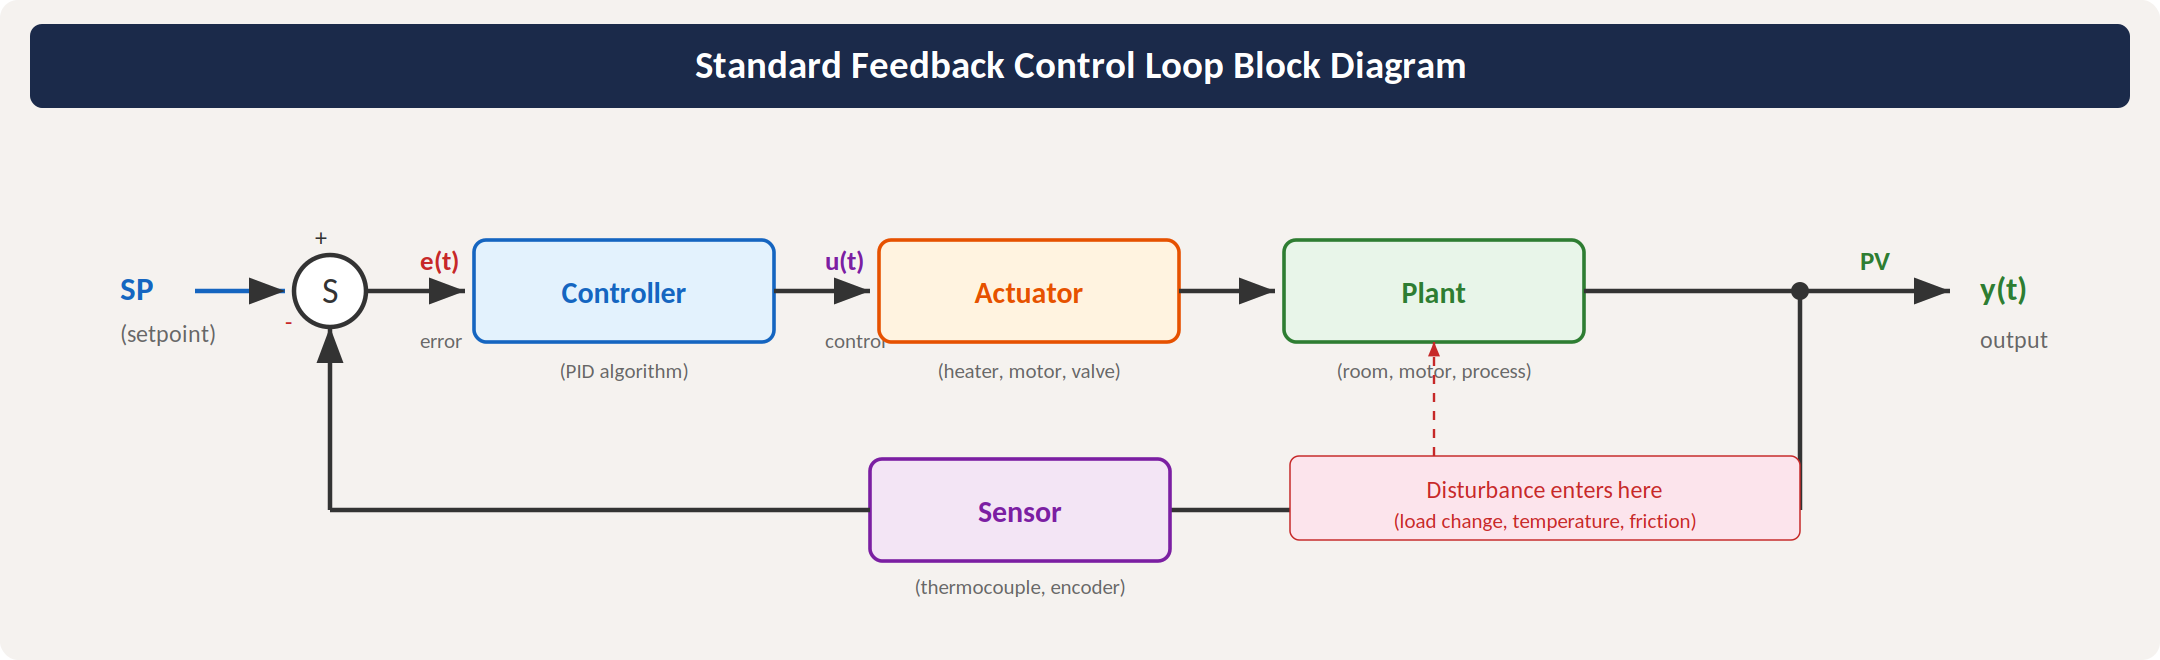
\includegraphics[width=\textwidth]{fig_feedback_loop.png}
\caption{Standard feedback control loop. The summing junction computes $e = \text{SP} - \text{PV}$. The controller processes the error and outputs a control signal $u(t)$. Disturbances enter at the plant, but the feedback loop detects and corrects their effect.}
\label{fig:feedback_loop}
\end{figure}

The summing junction computes $e = \text{SP} - \text{PV}$. The controller processes $e$ and outputs a control signal $u$. The actuator converts $u$ into physical action. The plant responds. The sensor measures the result and feeds it back.

\section{Advantages Over Open-Loop}
\begin{itemize}[leftmargin=1.5em]
\item \textbf{Disturbance rejection}: the controller compensates for unmeasured disturbances (load changes, supply voltage variations, environmental shifts).
\item \textbf{Reduced sensitivity to plant uncertainty}: the system works even if the plant model is imperfect.
\item \textbf{Improved accuracy}: steady-state error can be driven to zero (with integral action).
\end{itemize}

\section{Stability}
A feedback system can become \textbf{unstable} if the loop gain is too high or the phase shift around the loop reaches $-180$\ang{} at a frequency where the gain is still $>$1. An unstable system oscillates with growing amplitude. Stability analysis tools: Bode plots (gain and phase margins), root locus, and Nyquist criterion. For MEGN~300, the key takeaway is: excessive controller gain causes instability (oscillation).

\begin{tipbox}[The Stability Rule of Thumb]
If your controller output oscillates, the gain is too high. Reduce proportional gain first, then check if the oscillation stops. If the system responds sluggishly but does not oscillate, the gain may be too low.
\end{tipbox}


\section{Transfer Functions}
The transfer function $G(s)$ of a system relates its output to its input in the Laplace domain:
\begin{equation}
G(s) = \frac{Y(s)}{X(s)}
\end{equation}
For the standard closed-loop with forward path $G(s)$ and feedback sensor $H(s)$, the closed-loop transfer function is:
\begin{equation}
T(s) = \frac{G(s)}{1 + G(s)H(s)}
\end{equation}
The denominator $1 + G(s)H(s) = 0$ defines the \textbf{characteristic equation}; its roots determine stability. If any root has a positive real part, the system is unstable.

\section{Steady-State Error}
For a step input, the steady-state error depends on the \textbf{system type} (number of integrators in the open-loop transfer function):
\begin{itemize}[nosep,leftmargin=1.5em]
\item \textbf{Type 0} (no integrator, P-only): finite steady-state error $e_{ss} = 1/(1 + K_p)$ where $K_p$ is the DC loop gain.
\item \textbf{Type 1} (one integrator, PI or I controller): zero steady-state error for step inputs. This is why integral action eliminates offset.
\item \textbf{Type 2} (two integrators): zero steady-state error for step and ramp inputs.
\end{itemize}

\begin{keyconceptbox}[Requirements Mapping: Control Performance to Shall-Statements]
\begin{itemize}[nosep,leftmargin=1.5em]
\item ``Zero steady-state error'' $\to$ CTRL-REQ: The controller shall include integral action (PI or PID). Verify: step test showing error converges to within $\pm$[tolerance] of setpoint.
\item ``Rise time $<$2\,s, overshoot $<$10\%'' $\to$ CTRL-REQ: Step response shall reach 90\% of setpoint within 2\,s with peak overshoot $\leq$10\%. Verified by step test with data logging.
\item ``Gain margin $\geq$6\,dB, phase margin $\geq$45\ang{}'' $\to$ CTRL-REQ: Verified by Bode plot analysis of the open-loop transfer function.
\end{itemize}
\end{keyconceptbox}


\section{The Feedback Principle}
Closed-loop control measures the actual output (process variable, PV) and compares it to the desired output (setpoint, SP). The difference is the error: $e(t) = \text{SP} - \text{PV}$. The controller uses this error to compute a control action $u(t)$ that drives the error toward zero. This is the fundamental mechanism of all feedback control: measure, compare, correct.

\section{Closed-Loop Block Diagram Components}
\textbf{Setpoint (SP)}: the desired output value, specified by the user or a higher-level controller.

\textbf{Summing junction}: computes $e = \text{SP} - \text{PV}$.

\textbf{Controller}: processes the error $e$ to compute the control output $u$. May be as simple as a proportional gain or as sophisticated as a PID algorithm with anti-windup and derivative filtering.

\textbf{Actuator}: converts the control signal into physical action. Examples: heater (electrical power $\to$ heat), motor (electrical power $\to$ torque), valve (signal $\to$ flow rate).

\textbf{Plant}: the physical system being controlled (room temperature dynamics, motor speed dynamics, fluid level dynamics).

\textbf{Sensor}: measures the output of the plant and converts it to a signal for comparison with the setpoint. The sensor's accuracy, bandwidth, and noise directly limit the achievable control performance.

\textbf{Disturbance}: any uncontrolled influence that affects the plant output (door opening, load change, supply voltage fluctuation). Feedback detects the effect of the disturbance on the output and corrects for it.

\section{Transfer Functions and System Type}
A transfer function $G(s)$ describes the input-output relationship in the Laplace domain. The \textbf{open-loop transfer function} $L(s) = G_c(s) \cdot G_p(s)$ (controller times plant) determines the closed-loop behavior. The \textbf{system type} (number of pure integrators in $L(s)$) determines the steady-state error for different input types:

\textbf{Type 0} (no integrators): finite steady-state error for step inputs. $e_{ss} = 1/(1 + K_p)$ where $K_p = \lim_{s\to 0} L(s)$ is the position error constant. P-only control of a first-order plant is Type 0.

\textbf{Type 1} (one integrator): zero steady-state error for step inputs, finite for ramp inputs. PI control adds the required integrator.

\textbf{Type 2} (two integrators): zero steady-state error for step and ramp inputs. Rarely needed in instrumentation.

\section{Stability}
A closed-loop system is stable if and only if all poles of the closed-loop transfer function have negative real parts (lie in the left half of the $s$-plane). In practice, stability is assessed using gain margin (how much the gain can increase before instability) and phase margin (how much additional phase lag can be tolerated). For robust performance, aim for gain margin $> 6$\,dB and phase margin $> 45^\circ$.

\section{Closed-Loop Advantages}
\textbf{Disturbance rejection}: feedback detects and corrects the effect of disturbances. A door opening in a heated room causes a temperature drop that the controller detects and compensates by increasing heater power.

\textbf{Reduced sensitivity}: the closed-loop gain $T(s) = L(s)/(1+L(s))$ is much less sensitive to plant parameter variations than the open-loop gain. If the plant gain doubles, the closed-loop gain changes by a much smaller fraction.

\textbf{Integral action eliminates offset}: adding an integrator in the controller (the ``I'' in PID) drives the steady-state error to zero for step inputs, regardless of the plant's DC gain.


\section{Sensitivity and Complementary Sensitivity}
The closed-loop transfer function from setpoint to output is the \textbf{complementary sensitivity function} $T(s) = L(s)/(1+L(s))$ where $L(s) = G_c(s)G_p(s)$ is the open-loop transfer function. The \textbf{sensitivity function} $S(s) = 1/(1+L(s))$ describes how disturbances affect the output. Note that $S + T = 1$: you cannot simultaneously reduce sensitivity to disturbances at all frequencies. This is the fundamental limitation of feedback control.

At low frequencies where $|L| \gg 1$: $T \approx 1$ (output tracks setpoint), $S \approx 1/L \ll 1$ (disturbances are strongly rejected). At high frequencies where $|L| \ll 1$: $T \approx L \ll 1$ (output does not track fast setpoint changes), $S \approx 1$ (disturbances pass through unattenuated).

\section{Stability Margins in Detail}
\textbf{Gain margin}: the factor by which the loop gain can increase before the system becomes unstable. Measured at the frequency where the phase is $-180^\circ$. Minimum recommended: 6\,dB (gain can double before instability).

\textbf{Phase margin}: the additional phase lag the system can tolerate before instability. Measured at the gain crossover frequency (where $|L| = 1$). Minimum recommended: $45^\circ$. More phase margin gives less overshoot and more robust behavior.

In MEGN 300, you assess stability empirically: if the control loop oscillates, reduce $K_p$. If it oscillates with growing amplitude, you are at or beyond the stability boundary. Back off gain by at least 50\%.

\section{The Effect of Sensor Dynamics}
The sensor is inside the feedback loop. Its dynamic response (bandwidth, time constant) directly affects stability. A slow sensor adds phase lag, reducing the phase margin. For stable control, the sensor bandwidth should be at least $5\times$--$10\times$ the closed-loop bandwidth. If the sensor is too slow, the maximum achievable control bandwidth is limited by the sensor, not the controller or actuator.

\section{Disturbance Rejection Quantified}
For a step disturbance $d$ entering at the plant, the steady-state output deviation is:
\begin{equation}
\Delta y_{ss} = \frac{d}{1 + K_p K_{\text{plant}}} \quad \text{(P-only control)}
\end{equation}
With integral action (PI or PID), $\Delta y_{ss} = 0$ for step disturbances, because the integrator drives the error to zero regardless of the disturbance magnitude. This is the primary motivation for adding integral action.
\section{The Feedback Equation}
The closed-loop transfer function from setpoint $R(s)$ to output $Y(s)$:
\begin{equation}
T(s) = \frac{G_c(s)G_p(s)}{1 + G_c(s)G_p(s)H(s)}
\end{equation}
where $G_c$ is the controller, $G_p$ is the plant, and $H$ is the sensor/feedback transfer function. For an ideal sensor ($H = 1$): $T(s) = L(s)/(1+L(s))$ where $L(s) = G_c G_p$ is the loop transfer function.

At frequencies where $|L| \gg 1$ (low frequencies, typically): $T \approx 1/H \approx 1$ (output tracks setpoint regardless of plant dynamics). At frequencies where $|L| \ll 1$ (high frequencies): $T \approx L$ (no tracking; the bandwidth limit). The \textbf{crossover frequency} (where $|L| = 1$) defines the closed-loop bandwidth.

\section{Steady-State Error Analysis}
The steady-state error for a step input of magnitude $R_0$:
\begin{equation}
e_{ss} = \lim_{s \to 0} \frac{s \cdot R_0/s}{1 + L(s)} = \frac{R_0}{1 + K_p}
\end{equation}
where $K_p = \lim_{s \to 0} L(s)$ is the \textbf{position error constant}. For P-only control of a plant with DC gain $K_{\text{plant}}$: $K_p = K_p^{\text{ctrl}} \times K_{\text{plant}}$, and $e_{ss} = R_0/(1 + K_p^{\text{ctrl}} K_{\text{plant}})$.

Example: ThermoRig with $K_p^{\text{ctrl}} = 10$ and $K_{\text{plant}} = 1$\,\degC{}/\% power: $K_p = 10$, $e_{ss} = R_0/11 = 9.1\%$ of setpoint change. For a 50\,\degC{} setpoint (from 25\,\degC{} ambient): $e_{ss} = 25/11 = 2.3$\,\degC{}. The controller achieves 47.7\,\degC{} instead of 50\,\degC{}.

Adding integral action ($K_i > 0$) makes the system Type~1: $K_p \to \infty$, $e_{ss} \to 0$. This is the primary motivation for the ``I'' in PID.

\section{Stability Analysis Methods}
\subsection{Bode Plot Method}
Plot the magnitude and phase of $L(j\omega)$ vs.\ frequency. The system is stable if the gain margin (gain below 0\,dB at the $-180^\circ$ phase frequency) and phase margin (phase above $-180^\circ$ at the 0\,dB gain frequency) are both positive.

For the ThermoRig PI controller: $L(s) = (10 + 0.5/s) \times 1/(1+30s)$ (P$=10$, I$=0.5$, plant time constant $= 30$\,s). The Bode plot shows crossover at $\sim$0.05\,Hz with $\sim$50$^\circ$ phase margin. This is adequate ($>$45$^\circ$). Increasing $K_p$ to 20 reduces the phase margin to $\sim$30$^\circ$, making the response oscillatory.

\subsection{Root Locus (Conceptual)}
As the proportional gain $K_p$ increases from 0 to infinity, the closed-loop poles trace paths in the complex plane. When poles cross the imaginary axis, the system becomes unstable. Root locus shows the gain at which instability occurs (the ``ultimate gain'' $K_u$) and the frequency of oscillation ($f_u$). This is the theoretical basis for the Ziegler-Nichols tuning method.

\section{Performance Specifications}
\textbf{Rise time} ($t_r$): time for the output to go from 10\% to 90\% of the step change. Faster is better, but is limited by actuator power and stability.

\textbf{Overshoot} ($\%OS$): peak value above the setpoint, as a percentage of the step change. Typical target: $<$10\%. Zero overshoot requires overdamped response (slow settling).

\textbf{Settling time} ($t_s$): time for the output to remain within a specified band (typically $\pm$2\% or $\pm$5\%) of the final value. For a second-order system: $t_s \approx 4/(\zeta \omega_n)$.

\textbf{Steady-state error} ($e_{ss}$): final deviation from setpoint. Zero with integral action for step inputs.

These four specifications are mutually constrained: reducing rise time increases overshoot (for a given plant and controller structure). Achieving zero steady-state error (integral action) increases overshoot and settling time. The controller gains represent a tradeoff among these competing objectives.

\section{Practical Closed-Loop Design Steps}
(1) Characterize the plant: apply a step input in open loop and measure the output response. Fit a first or second-order model. For the ThermoRig: $G_p(s) \approx K/(1+\tau s) = 1/(1+30s)$ (first-order with $\tau = 30$\,s).

(2) Choose a controller structure: P, PI, or PID. For systems requiring zero steady-state error: PI minimum. For systems with significant overshoot: add D.

(3) Tune the controller: Z-N method for initial gains, then manual refinement based on step response observation.

(4) Verify stability and performance: check phase margin ($>$45$^\circ$), overshoot ($<$10\%), settling time (within specification), and steady-state error (zero for step inputs with integral action).

(5) Test robustness: change the plant conditions (different ambient temperature, different load, different supply voltage) and verify the controller still performs acceptably.
\section{Closed-Loop Bandwidth and Speed of Response}
The closed-loop bandwidth $f_{BW}$ determines how fast the system can track changing setpoints and reject disturbances. For a first-order closed-loop system: $f_{BW} = f_{-3\text{dB}} = (1+K_p K_{\text{plant}}) / (2\pi\tau)$, where $\tau$ is the plant time constant. Higher gain $K_p$ increases bandwidth (faster response), but also reduces stability margins.

For the ThermoRig with $K_p = 10$, $K_{\text{plant}} = 1$, $\tau = 30$\,s: $f_{BW} = 11/(2\pi \times 30) = 0.058$\,Hz, corresponding to a closed-loop time constant of $30/11 = 2.7$\,s (much faster than the open-loop 30\,s). With $K_p = 50$: $f_{BW} = 0.27$\,Hz, closed-loop time constant $= 0.59$\,s. But the phase margin at this gain may be insufficient.

\section{The Sensitivity Tradeoff}
The sensitivity function $S(s) = 1/(1 + L(s))$ and the complementary sensitivity function $T(s) = L(s)/(1+L(s))$ satisfy $S + T = 1$ at every frequency. This means: at frequencies where the system tracks the setpoint well ($|T| \approx 1$), it also rejects disturbances well ($|S| \approx 0$). At frequencies where tracking is poor ($|T| \approx 0$), disturbances pass through unattenuated ($|S| \approx 1$).

The crossover frequency (where $|L| = 1$) separates these two regimes. Below crossover: good tracking and disturbance rejection. Above crossover: no tracking, no disturbance rejection. This is why increasing bandwidth (moving the crossover to higher frequencies) improves performance, subject to the stability constraint.

\section{Effect of Time Delay (Dead Time)}
Dead time $L$ in the plant ($G_p(s) = K e^{-Ls}/(1+\tau s)$) introduces phase lag $\phi = -\omega L$ radians at frequency $\omega$, without affecting magnitude. This phase lag directly reduces the phase margin: $\Delta PM = -360 \times f_{BW} \times L$ degrees. For the ThermoRig with $L = 3$\,s and $f_{BW} = 0.058$\,Hz: $\Delta PM = -360 \times 0.058 \times 3 = -63$\degC{}. This is very significant; the dead time alone uses most of the available phase budget.

Dead time is the enemy of feedback control. It limits the achievable bandwidth and the maximum usable gain. Systems with large $L/\tau$ ratios (dead time comparable to the time constant) are inherently difficult to control. The Smith predictor is an advanced control technique that compensates for dead time by including a model of the plant (including its delay) inside the controller.

\section{Integral Action and Reset Windup}
When integral action is added ($K_i > 0$), the steady-state error for step inputs becomes zero. However, integral action has two drawbacks:

(1) \textbf{Reduced stability}: the integrator adds $-90$\degC{} of phase lag at all frequencies, reducing the phase margin. If the original P-only system had 60\degC{} phase margin, adding integral action might reduce it to 30\degC{} or less, producing oscillatory behavior. The solution: reduce $K_i$ (longer integral time $T_i$) to push the integral action to lower frequencies where its phase contribution at the crossover frequency is minimized.

(2) \textbf{Integral windup}: when the actuator saturates, the integral continues to accumulate, causing massive overshoot when the error changes sign. This is addressed in Chapter~16.
\section{Root Locus: Physical Interpretation}
The root locus is a graphical tool showing how the closed-loop pole locations change as the proportional gain $K_p$ varies from 0 to infinity. Each pole traces a path (locus) in the complex plane. The pole locations determine the dynamic behavior:

\textbf{Real-axis poles}: produce exponential modes. A pole at $s = -a$ produces a mode $e^{-at}$ with time constant $\tau = 1/a$. More negative $=$ faster decay.

\textbf{Complex conjugate poles}: produce oscillatory modes. Poles at $s = -\sigma \pm j\omega_d$ produce $e^{-\sigma t}\sin(\omega_d t + \phi)$. The real part $\sigma$ determines the decay rate; the imaginary part $\omega_d$ determines the oscillation frequency.

\textbf{Imaginary axis poles}: produce sustained oscillation (marginally stable). This is the ultimate gain $K_u$: the gain at which poles reach the imaginary axis. Beyond this gain: poles enter the right half-plane and the system is unstable.

For the ThermoRig FOPDT model $G_p(s) = 1.1 e^{-3s}/(1+30s)$ with PI controller $G_c(s) = K_p(1 + 1/(T_i s))$: as $K_p$ increases, the dominant poles move from the real axis (overdamped at low gain) toward the imaginary axis (oscillatory at high gain), crossing at $K_u \approx 35$. The Ziegler-Nichols tuning sets $K_p = 0.45 K_u = 15.75$, which places the poles roughly halfway between the real axis and the imaginary axis, giving a damped oscillatory response with $\sim$25\% overshoot.

\section{Frequency-Domain Design: Lead and Lag Compensation}
Beyond PID, classical control design uses \textbf{lead compensators} (to add phase and increase bandwidth) and \textbf{lag compensators} (to increase low-frequency gain for steady-state accuracy without affecting stability).

\textbf{Lead compensator}: $G_{\text{lead}}(s) = K_c \cdot (s + z)/(s + p)$ where $p > z$ (pole at higher frequency than zero). Adds positive phase near the geometric mean of $z$ and $p$. Use when you need more phase margin at the crossover frequency.

\textbf{Lag compensator}: $G_{\text{lag}}(s) = K_c \cdot (s + z)/(s + p)$ where $z > p$ (zero at higher frequency than pole). Adds gain at low frequencies (improving steady-state accuracy) without significantly affecting the crossover frequency or phase margin.

In MEGN~300, the PI controller is a lag compensator (the integrator adds infinite gain at DC), and the PD controller is a lead compensator (the derivative adds phase at the crossover frequency). The PID combines both.

\section{Closed-Loop Response to Ramp Inputs}
Many control applications require tracking a ramping setpoint (heating at a constant rate, constant-speed motion). The steady-state tracking error for a ramp input $r(t) = Rt$ depends on the system type:

Type 0 (P-only): ramp error grows without bound. P-only cannot track a ramp.

Type 1 (PI): finite ramp error $e_{ss} = R/K_v$ where $K_v = \lim_{s \to 0} sL(s)$ is the velocity error constant. Higher $K_v$ (higher integral gain) reduces the ramp tracking error.

Type 2 (PID with double integrator): zero ramp error. However, double integrators are difficult to stabilize and are rarely needed in thermal or mechanical systems.

For the ThermoRig ramping at 1\,\degC{}/s with PI control ($K_v = K_p K_i K_{\text{plant}} = 10 \times 0.5 \times 1.1 = 5.5$\,s$^{-1}$): $e_{ss} = 1.0/5.5 = 0.18$\,\degC{}. The temperature always lags the ramp by 0.18\,\degC{}. Increasing $K_i$ reduces this lag but increases overshoot at the end of the ramp.

\section{Implementation Considerations}
\textbf{Sampling rate selection}: the control loop update rate should be $\geq 10\times$ the closed-loop bandwidth. For the ThermoRig ($f_{BW} \approx 0.05$\,Hz): $f_s \geq 0.5$\,Hz ($T_s \leq 2$\,s). We use $T_s = 100$\,ms ($f_s = 10$\,Hz) for margin. For motor speed control ($f_{BW} = 100$\,Hz): $f_s \geq 1$\,kHz.

\textbf{Computational delay}: the time between reading the sensor and writing the actuator output. In LabVIEW on a desktop PC: 1--10\,ms (adequate for thermal and slow mechanical systems). On a real-time controller (CompactRIO, myRIO): $< 100\,\mu$s. On a microcontroller (ESP32): $< 1$\,ms. Computational delay adds to the dead time and reduces phase margin.

\textbf{Actuator saturation}: every actuator has limits (heater: 0--100\%, motor: $-V_{\text{max}}$ to $+V_{\text{max}}$). The controller's output must be clamped to the actuator range. Saturation means the controller temporarily loses authority: it commands more than the actuator can deliver. During saturation, the feedback loop is effectively broken, and integral windup can occur (addressed in the PID chapter).
\section{Practice Questions}
\begin{enumerate}[leftmargin=1.5em]
\item Draw the block diagram for a closed-loop temperature control system. Label: setpoint, error, controller, heater (actuator), room (plant), and temperature sensor. Identify a specific disturbance and show where it enters the loop.
\item Explain why a thermostat (on/off controller) is a closed-loop system, and identify what limits its accuracy.
\item Your closed-loop motor speed controller oscillates at 5\,Hz. What is the most likely cause, and what is the first adjustment you should make?
\end{enumerate}

\subsection{Answers}
\begin{enumerate}[leftmargin=1.5em]
\item Block diagram: SP (desired temp) $\to$ summing junction $\to$ PID controller $\to$ relay/SSR (actuator) $\to$ room (plant) $\to$ PV (room temperature) $\to$ temperature sensor (e.g., thermistor) $\to$ feedback to summing junction. Disturbance: someone opens a window (heat loss), which enters between the plant and the output.
\item A thermostat measures the room temperature (feedback), compares it to the setpoint, and switches the heater on or off. It is closed-loop because the output (temperature) is measured and used to determine the control action. Accuracy is limited by: (1) the dead band (hysteresis) between the on and off thresholds, (2) the sensor's accuracy and placement, and (3) the thermal lag between the heater and the sensor location.
\item The oscillation indicates the loop gain exceeds the stability margin at 5\,Hz. First adjustment: reduce the proportional gain ($K_p$) by 50\% and observe if the oscillation amplitude decreases. If it stops, the gain was too high. If it persists, check for measurement delay (sensor lag, DAQ sampling latency) that adds phase shift to the loop.
\end{enumerate}


% ================================================================
\chapter{PID Control}

\section{The PID Controller}
The Proportional-Integral-Derivative controller is the most widely used feedback controller in industry. The control output is:
\begin{equation}
u(t) = K_p \, e(t) + K_i \int_0^t e(\tau)\, d\tau + K_d \frac{de(t)}{dt}
\end{equation}
where $e(t) = \text{SP} - \text{PV}$ is the error.

\section{The Three Terms}

\subsection{Proportional (P)}
$u_P = K_p \cdot e(t)$. Output is directly proportional to the current error. Higher $K_p$ gives faster response but more overshoot. \textbf{P-only control always has steady-state error} (called ``offset'') because the controller needs a nonzero error to produce a nonzero output.

\subsection{Integral (I)}
$u_I = K_i \int e(\tau)\, d\tau$. Output is proportional to the accumulated error over time. The integral term \textbf{eliminates steady-state error}: as long as any error exists, the integral grows, increasing the output until the error reaches zero. Too much integral action causes overshoot and oscillation (slow, wind-up driven).

\subsection{Derivative (D)}
$u_D = K_d \cdot de/dt$. Output is proportional to the rate of change of error. The derivative term provides \textbf{damping}: it opposes rapid changes, reducing overshoot and improving stability. Sensitive to noise (differentiating a noisy signal amplifies the noise); usually low-pass filtered in practice.

\begin{figure}[htbp]
\centering
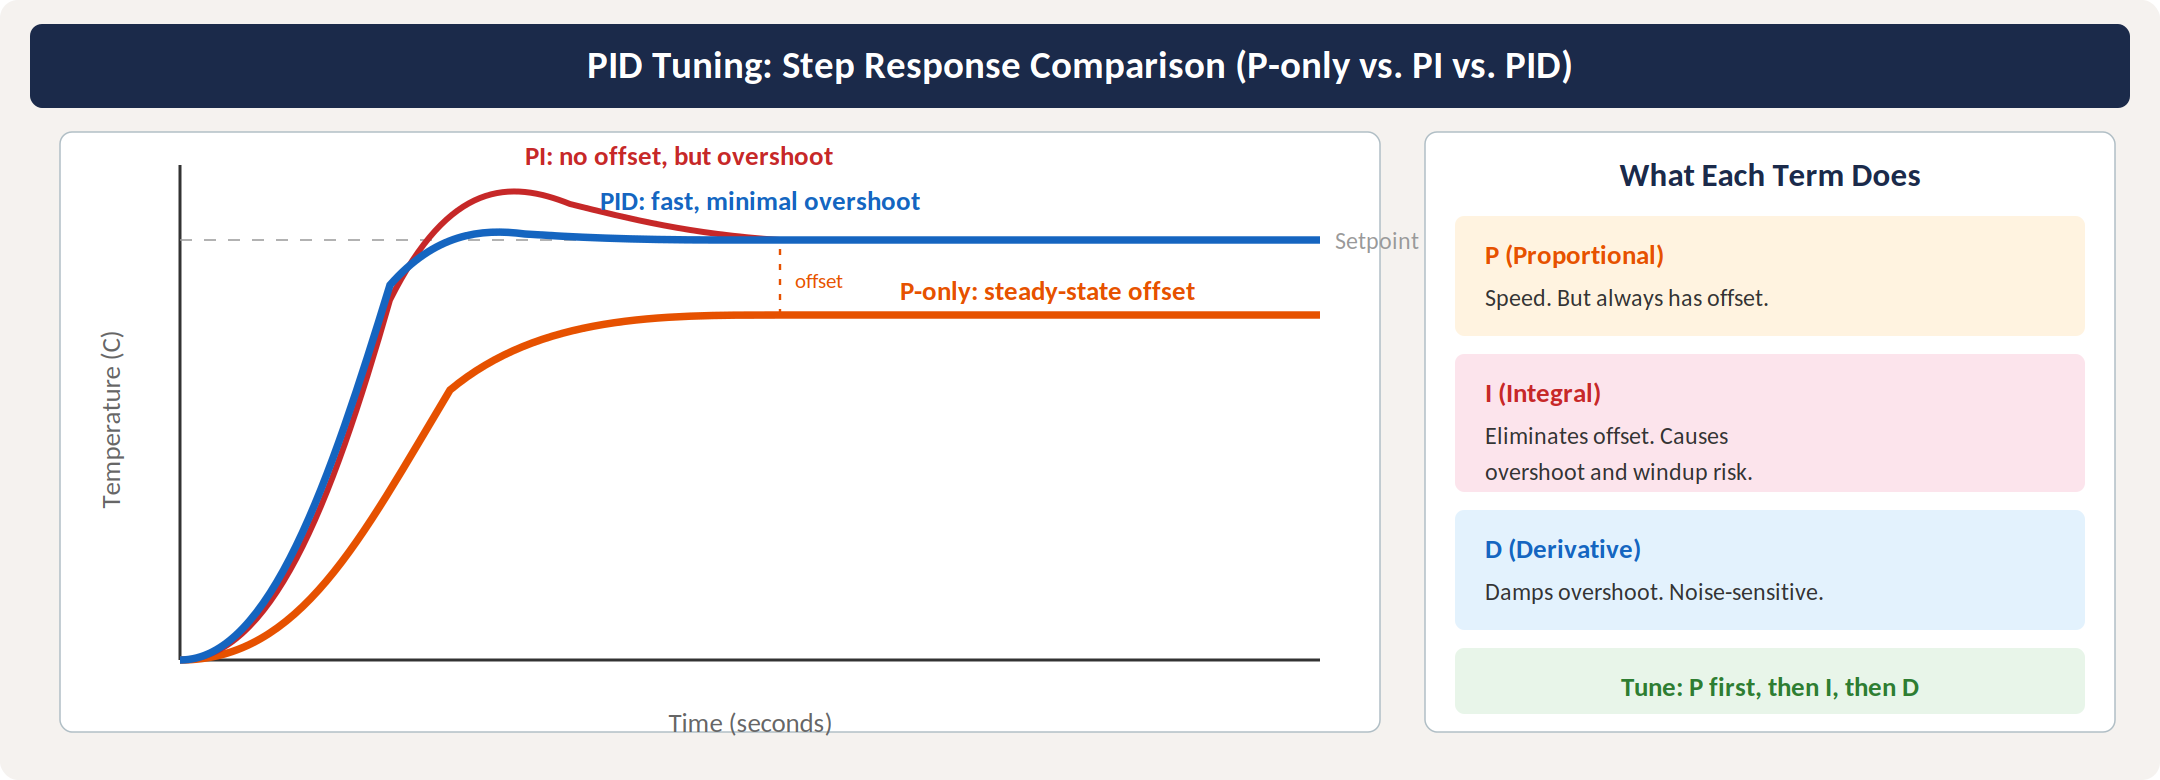
\includegraphics[width=\textwidth]{fig_pid_step_responses.png}
\caption{Step response comparison: P-only (steady-state offset), PI (offset eliminated but overshoot), PID (fast settling, minimal overshoot). Tune P first for speed, add I for accuracy, add D for damping.}
\label{fig:pid_steps}
\end{figure}

\begin{figure}[htbp]
\centering
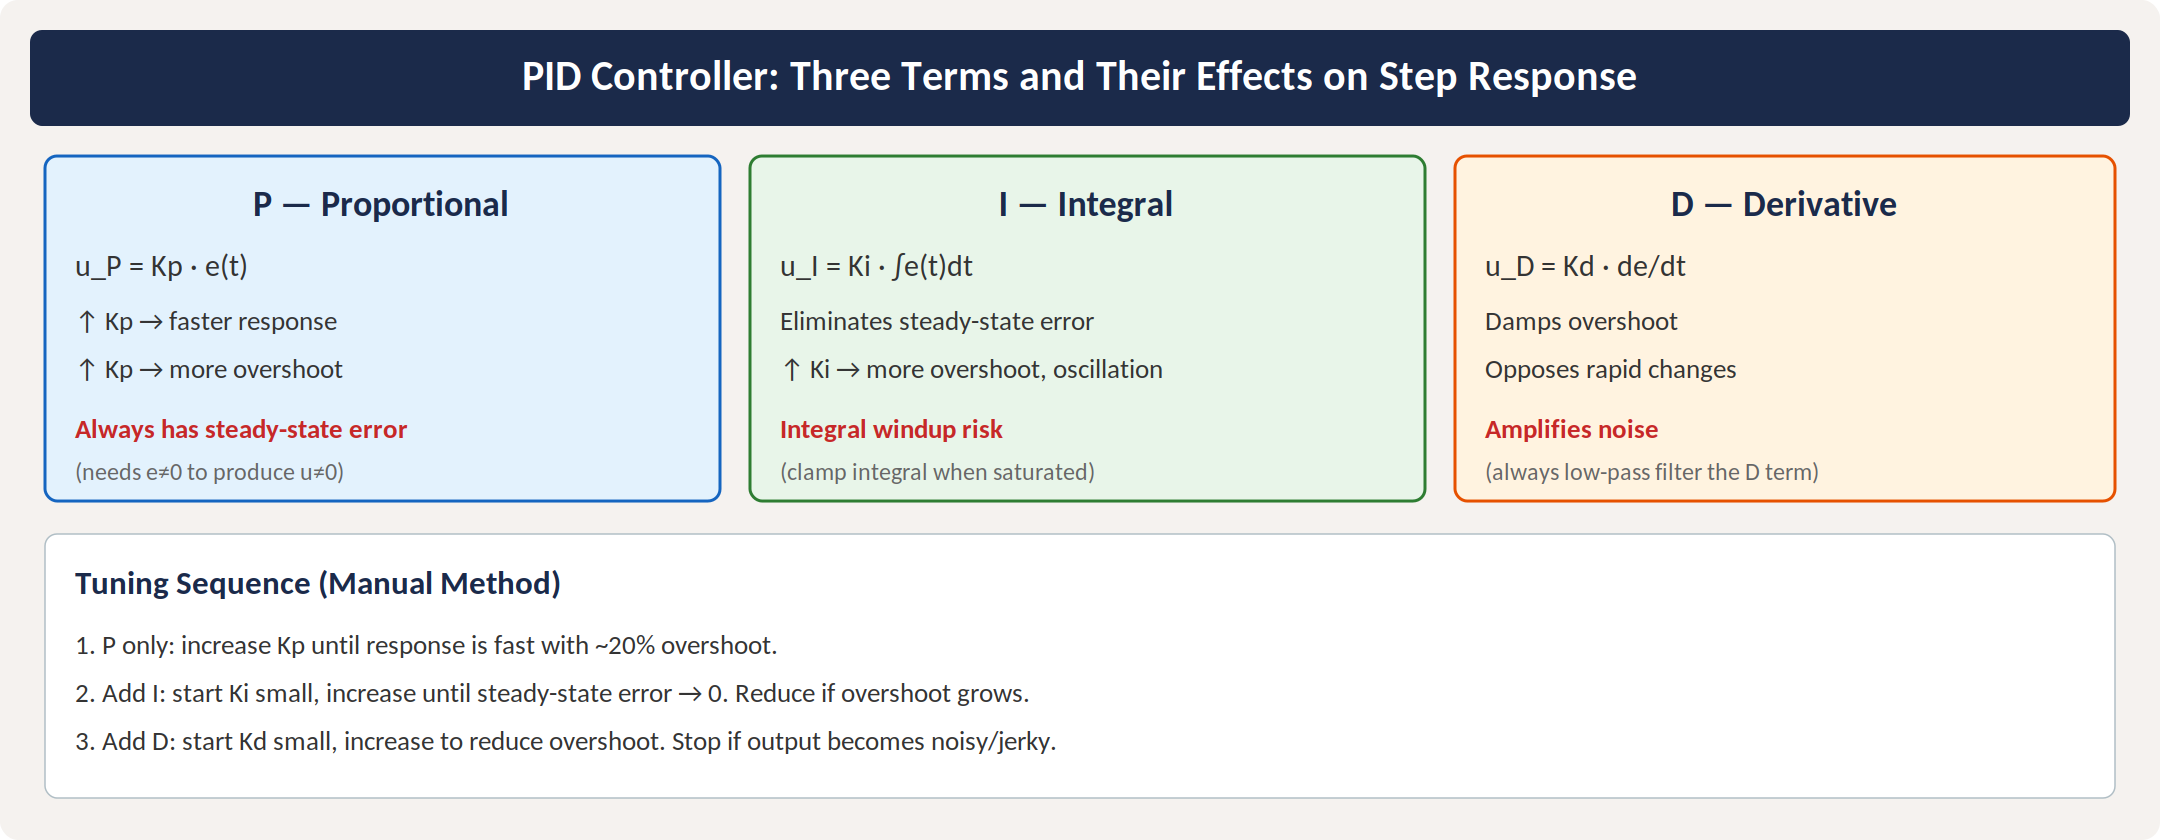
\includegraphics[width=\textwidth]{fig_pid_terms.png}
\caption{The three PID controller terms, their effects, risks, and the manual tuning sequence.}
\label{fig:pid}
\end{figure}

\begin{examplebox}[ThermoRig: PID Temperature Control]
The ThermoRig controls a 100\,W cartridge heater to maintain a metal block at a setpoint temperature. The sensor is a Type~K thermocouple read by the NI~DAQ at 10\,S/s.

\textbf{P-only} ($K_p = 5$\,\%/\degC{}): the heater reaches 95\% of setpoint but stabilizes with a 2.5\,\degC{} offset below target.

\textbf{PI} ($K_p = 5$, $K_i = 0.5$\,\%/(\degC{}$\cdot$s)): the offset is eliminated; the system reaches setpoint in 45\,s with 8\% overshoot.

\textbf{PID} ($K_p = 5$, $K_i = 0.5$, $K_d = 2$\,\%$\cdot$s/\degC{}): overshoot reduced to 2\%, settling time 30\,s. The derivative term damps the approach to setpoint.
\end{examplebox}


\section{From PID Output to Physical Actuator}
The PID controller computes a control variable $u(t)$ as a percentage (0--100\%). This abstract number must be converted into a physical actuation signal:

\textbf{For a DC motor} (speed control): $u$ maps to PWM duty cycle. At $u = 50\%$, the MOSFET switches the motor supply at 50\% duty, delivering half the average voltage. The PWM frequency (1--25\,kHz) is fast enough that the motor's inertia smooths the pulsed current.

\textbf{For an AC heater} (temperature control via SSR): $u$ maps to time-proportional control. Over a fixed period (e.g., 1\,s), the SSR is ON for $u/100 \times 1$\,s and OFF for the remainder. At $u = 75\%$, the heater is ON for 0.75\,s and OFF for 0.25\,s each cycle. The thermal mass of the system smooths this into quasi-continuous heating.

\textbf{For a valve} (flow/pressure control): $u$ maps to valve position via a servo actuator or stepper motor driving the valve stem.

In LabVIEW, wire the PID output (0--100) to a ``Rescale'' function that converts to the appropriate DAQ output: a 0--3.3\,V analog voltage for a proportional driver, or a digital output with timing logic for time-proportional SSR control.

\begin{keyconceptbox}[Requirements Mapping: Control Output to Shall-Statements]
\begin{itemize}[nosep,leftmargin=1.5em]
\item ``PID loop rate $\geq$10\,Hz'' $\to$ SW-REQ: LabVIEW While Loop period shall be $\leq$100\,ms, verified by timing measurement.
\item ``Heater PWM resolution $\leq$1\%'' $\to$ HW-REQ: Time-proportional period shall be $\geq$1\,s (giving 100 discrete steps at 10\,ms resolution).
\item ``Motor speed controllable 0--100\%'' $\to$ HW-REQ: PWM duty cycle shall span 0--100\% with $\geq$8-bit resolution (256 steps).
\end{itemize}
\end{keyconceptbox}

\section{Tuning Methods}

\subsection{Ziegler-Nichols (Closed-Loop)}
\begin{enumerate}[nosep,leftmargin=1.5em]
\item Set $K_i = 0$ and $K_d = 0$ (P-only control).
\item Increase $K_p$ until the system oscillates at a constant amplitude. Record this \textbf{ultimate gain} $K_u$ and the \textbf{ultimate period} $T_u$.
\item Apply the Ziegler-Nichols tuning rules:
\end{enumerate}
\begin{table}[htbp]\centering\small
\begin{tabularx}{0.7\textwidth}{l c c c}
\toprule
\textbf{Controller} & $K_p$ & $T_i$ & $T_d$ \\
\midrule
P & $0.50 \, K_u$ & -- & -- \\
PI & $0.45 \, K_u$ & $T_u / 1.2$ & -- \\
PID & $0.60 \, K_u$ & $T_u / 2.0$ & $T_u / 8.0$ \\
\bottomrule
\end{tabularx}
\caption{Ziegler-Nichols closed-loop tuning rules. $K_i = K_p / T_i$, $K_d = K_p \cdot T_d$.}
\end{table}

\subsection{Manual Tuning}
\begin{enumerate}[nosep,leftmargin=1.5em]
\item Start with P-only. Increase $K_p$ until the response is reasonably fast with acceptable overshoot (typically 10--25\%).
\item Add integral. Start $K_i$ small; increase until the steady-state error is eliminated. If overshoot increases significantly, reduce $K_i$.
\item Add derivative. Start $K_d$ small; increase to reduce overshoot and oscillation. If the output becomes jerky or noisy, $K_d$ is too high.
\end{enumerate}

\section{Integral Windup}
When the actuator saturates (e.g., heater at 100\% duty, valve fully open), the error persists and the integral term continues to grow. When the error finally reverses, the large integral value causes excessive overshoot before the integral ``unwinds.'' \textbf{Anti-windup}: stop integrating when the actuator is saturated, or clamp the integral term to a maximum value.

\begin{figure}[htbp]
\centering
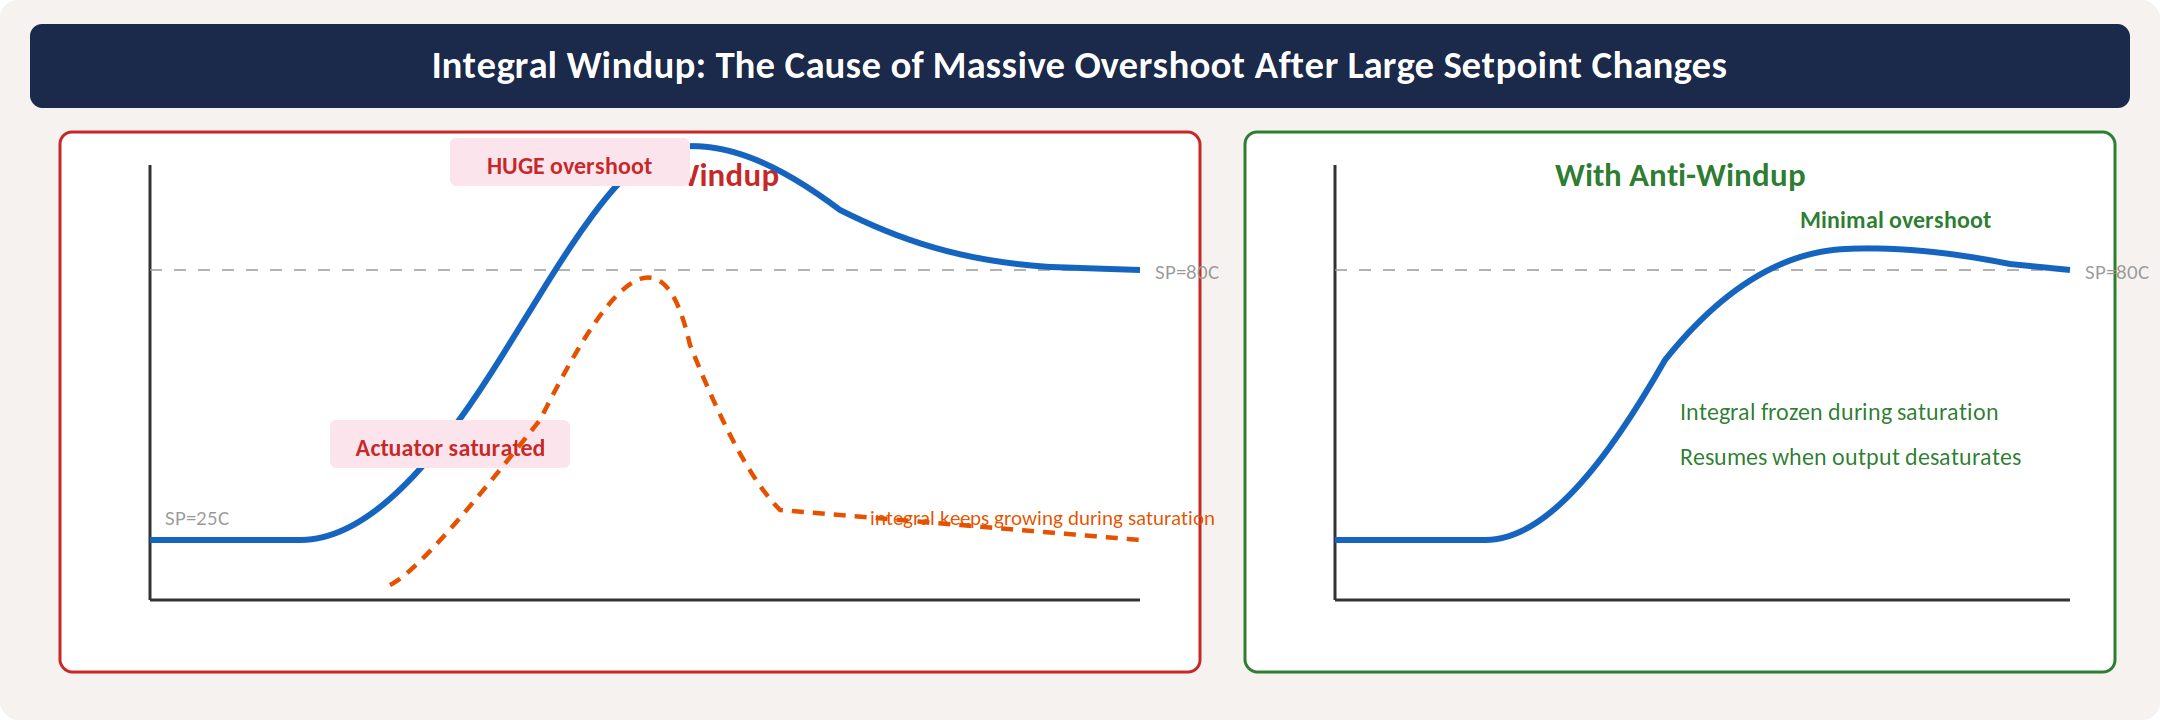
\includegraphics[width=\textwidth]{fig_integral_windup.png}
\caption{Integral windup: without anti-windup (left), the integral term accumulates during actuator saturation, causing massive overshoot. With anti-windup (right), the integral is frozen during saturation, producing minimal overshoot.}
\label{fig:windup}
\end{figure}

\section{Digital PID Implementation}
In discrete time (sampling period $T_s$):
\begin{align}
u[n] &= K_p \, e[n] + K_i \, T_s \sum_{k=0}^{n} e[k] + K_d \, \frac{e[n] - e[n-1]}{T_s}
\end{align}
This is the \textbf{positional form}. The \textbf{velocity form} computes the change in output ($\Delta u$) instead of the absolute value, which naturally prevents integral windup:
\begin{equation}
\Delta u[n] = K_p (e[n] - e[n-1]) + K_i T_s \, e[n] + K_d \frac{e[n] - 2e[n-1] + e[n-2]}{T_s}
\end{equation}

\begin{keyconceptbox}[Requirements Mapping: PID to Shall-Statements]
\begin{itemize}[nosep,leftmargin=1.5em]
\item ``Maintain temperature at setpoint $\pm$0.5\,\degC{}'' $\to$ CTRL-REQ: PID controller shall achieve steady-state error $\leq$0.5\,\degC{} within 60\,s of a step change.
\item ``No overshoot $>$5\%'' $\to$ CTRL-REQ: Step response overshoot shall be $\leq$5\% of the step magnitude.
\item ``Control loop executes at $\geq$10\,Hz'' $\to$ SW-REQ: PID computation and DAQ cycle shall complete within 100\,ms.
\end{itemize}
\end{keyconceptbox}


\section{Practical PID Considerations}

\subsection{Derivative Filter}
The pure derivative term $K_d \cdot de/dt$ amplifies high-frequency noise. In practice, the derivative is always filtered:
\begin{equation}
u_D(s) = \frac{K_d s}{1 + \frac{s}{N \omega_c}} \quad \text{where } N = 2\text{--}20
\end{equation}
This limits the derivative gain at high frequencies. In discrete form: use a first-order low-pass on the error difference before multiplying by $K_d$. LabVIEW's PID VI includes this filter automatically.

\subsection{Setpoint Weighting}
When the setpoint changes suddenly (step change), the proportional and derivative terms produce a large instantaneous output (``derivative kick''). Setpoint weighting reduces this: apply P and D only to the process variable (not the error), while I acts on the full error. This gives smooth response to setpoint changes while maintaining full disturbance rejection.

\subsection{Bumpless Transfer}
When switching between manual and automatic control modes, a poorly implemented PID can produce a large output jump. Bumpless transfer initializes the integral term so that the automatic output matches the manual output at the moment of transfer.

\subsection{Cascade Control}
For systems with multiple time constants (e.g., a heater heating a metal block that heats a fluid), cascade control uses two nested loops: an inner (fast) loop controls the heater temperature, and an outer (slow) loop controls the fluid temperature. The outer loop's output becomes the inner loop's setpoint. This rejects disturbances faster by addressing them at the inner loop before they propagate to the outer variable.

\begin{examplebox}[ThermoRig: Complete PID Implementation in LabVIEW]
The ThermoRig PID loop runs at 10\,Hz ($T_s = 0.1$\,s). The NI DAQ reads the thermocouple (averaged over 10 readings per cycle for noise reduction). The PID VI computes the output (0--100\% duty cycle). The output drives the SSR via a digital output toggled at 1\,Hz time-proportional rate.

Tuning: Ziegler-Nichols yielded $K_u = 15$, $T_u = 8$\,s. Z-N PID: $K_p = 9.0$, $K_i = 2.25$/s, $K_d = 2.25$\,s. After manual refinement (reducing overshoot): $K_p = 6.0$, $K_i = 1.5$/s, $K_d = 3.0$\,s. Anti-windup enabled with integral clamp at $\pm$50\%. Result: setpoint reached in 35\,s, overshoot 3\%, steady-state error $<$0.2\,\degC{}.
\end{examplebox}


\section{PID Controller Theory}
The PID (Proportional-Integral-Derivative) controller computes the control output as:
\begin{equation}
u(t) = K_p \, e(t) + K_i \int_0^t e(\tau)\,d\tau + K_d \frac{de(t)}{dt}
\end{equation}
where $e(t) = \text{SP} - \text{PV}$ is the error. Each term contributes a distinct behavior:

\subsection{Proportional (P) Term}
$u_P = K_p \cdot e$: output proportional to current error. Higher $K_p$ gives faster response but more overshoot and less stability margin. P-only control always has a non-zero steady-state error (offset) for step inputs in Type~0 systems:
\begin{equation}
e_{ss} = \frac{1}{1 + K_p K_{\text{plant}}}
\end{equation}
For $K_p = 10$ and $K_{\text{plant}} = 1$: $e_{ss} = 1/11 \approx 9.1\%$ of the step size. Higher $K_p$ reduces but never eliminates the offset.

\subsection{Integral (I) Term}
$u_I = K_i \int e\,dt$: output proportional to the accumulated error over time. The integral action eliminates steady-state offset by continuously increasing the output as long as any error persists. However, it introduces phase lag (reduces stability) and can cause \textbf{integral windup} when the actuator saturates.

\subsection{Derivative (D) Term}
$u_D = K_d \cdot de/dt$: output proportional to the rate of change of error. It provides predictive action, reducing overshoot and improving stability by ``braking'' when the error is decreasing rapidly. However, it amplifies high-frequency noise. In practice, the derivative is computed from the PV (not the error) to avoid setpoint step spikes, and a low-pass filter is applied to the derivative signal.

\section{Tuning Methods}
\subsection{Ziegler-Nichols Closed-Loop Method}
(1) Set $K_i = 0$ and $K_d = 0$ (P-only). (2) Increase $K_p$ until the system oscillates at constant amplitude. Record this $K_p$ as $K_u$ (ultimate gain) and the oscillation period as $T_u$ (ultimate period). (3) Calculate gains from the Z-N table:

P-only: $K_p = 0.5 K_u$. PI: $K_p = 0.45 K_u$, $T_i = T_u/1.2$. PID: $K_p = 0.6 K_u$, $T_i = T_u/2$, $T_d = T_u/8$.

Z-N tuning produces aggressive response with significant overshoot ($\sim$25\%). Use it as a starting point and manually reduce $K_p$ and increase $T_i$ for less aggressive behavior.

\subsection{Manual Tuning}
(1) Set $K_i = 0$, $K_d = 0$. Increase $K_p$ until the response is fast with acceptable overshoot ($<$10\%). (2) Gradually increase $K_i$ to eliminate the steady-state offset. Too much $K_i$ causes slow oscillation. (3) Add $K_d$ to reduce overshoot and improve settling. Too much $K_d$ causes high-frequency jitter (noise amplification).

\section{Anti-Windup}
When the actuator saturates (e.g., heater at 100\% power), the integral term continues to accumulate error, growing very large. When the error finally changes sign, the massive accumulated integral drives the output far past the setpoint, causing enormous overshoot. This is \textbf{integral windup}.

The clamping anti-windup strategy: when the output hits the actuator limit, stop accumulating the integral. Resume integration only when the output comes back within the actuator's range. The pseudocode in Section~16.4 implements this.

\section{Discrete PID Implementation}
In LabVIEW (or any digital controller), the continuous PID equation is discretized:
\begin{equation}
u[n] = K_p \, e[n] + K_i \, T_s \sum_{k=0}^{n} e[k] + \frac{K_d}{T_s}\left(e[n] - e[n-1]\right)
\end{equation}
where $T_s$ is the sample period. The integral is a running sum (stored in a shift register). The derivative is a first difference (also using a shift register for $e[n-1]$). Anti-windup: if the output exceeds actuator limits, do not update the integral sum.

\begin{examplebox}[ThermoRig: PID Tuning for Temperature Control]
The ThermoRig heater drives a 200\,W ceramic element through an SSR. Using Z-N method: with PI control only, we increase $K_p$ until sustained oscillation at $K_u = 35$, $T_u = 18$\,s. Z-N PI: $K_p = 15.75$, $T_i = 15$\,s ($K_i = K_p/T_i = 1.05$). This produces 22\% overshoot. Manual refinement: reduce $K_p$ to 10, increase $T_i$ to 20\,s ($K_i = 0.5$), add $K_d = 5$ with a derivative filter at 10\,Hz. Result: 4\% overshoot, 45\,s settling to $\pm$0.5\,\degC{} of the 80\,\degC{} setpoint. Anti-windup clamping active during large setpoint changes.
\end{examplebox}

\section{Practical PID Tips}
\textbf{Derivative on PV, not error}: compute $K_d \cdot d(\text{PV})/dt$ instead of $K_d \cdot de/dt$. This avoids the derivative spike that occurs when the setpoint changes step-wise.

\textbf{Derivative filter}: a first-order LP filter on the derivative term with cutoff at $5$--$10\times$ the closed-loop bandwidth. Without it, sensor noise is amplified by the derivative gain.

\textbf{Sampling rate}: the PID loop rate must be at least $10\times$ the closed-loop bandwidth. For a system with 5\,s settling time (bandwidth $\sim$0.2\,Hz), the loop should update at $\geq$2\,Hz ($T_s \leq 0.5$\,s). Faster is better; 10--100\,Hz is typical for thermal systems.

\textbf{Bumpless transfer}: when switching from manual to automatic mode, initialize the integral term to the current manual output to avoid an output jump.


\section{PID Gain Units and Conversion}
Different PID implementations use different parameterizations. The \textbf{parallel (independent)} form: $u = K_p e + K_i \int e\,dt + K_d de/dt$, with units $K_p$\,[output/error], $K_i$\,[output/(error$\cdot$s)], $K_d$\,[output$\cdot$s/error].

The \textbf{standard (ISA)} form: $u = K_c\left(e + \frac{1}{T_i}\int e\,dt + T_d \frac{de}{dt}\right)$, where $K_c = K_p$ is the controller gain, $T_i = K_p/K_i$ is the integral time (seconds), and $T_d = K_d/K_p$ is the derivative time (seconds). Many industrial controllers and LabVIEW's PID VI use the ISA form.

Conversion: $K_i = K_c/T_i$ and $K_d = K_c \times T_d$. When reading Z-N tuning tables or textbook examples, verify which form is used before entering the gains.

\section{Cascade Control}
For systems with multiple time constants (e.g., a heater inside an insulated chamber: fast heater response, slow chamber response), a single PID loop may not provide adequate performance. \textbf{Cascade control} uses two nested loops: an inner (fast) loop controls the heater temperature, and an outer (slow) loop controls the chamber temperature by setting the setpoint for the inner loop. The inner loop rejects disturbances (supply voltage changes) before they propagate to the outer loop, dramatically improving the overall response.

\section{Feed-Forward Combined with PID}
The PID controller corrects for errors after they occur (reactive). A feed-forward term can anticipate known disturbances and act before the error appears (proactive). For the ThermoRig: measuring the door-open event with a switch and immediately increasing heater power by a predetermined amount (feed-forward), while the PID handles the residual error (feedback). The combined system responds faster to disturbances than either approach alone.
\section{PID Autotuning}
Manual PID tuning requires expertise and time. \textbf{Autotuning} algorithms automate the process:

\textbf{Relay feedback method} (Astrom-Hagglund): replace the controller with a relay (bang-bang controller). The system oscillates at the ultimate frequency with the relay amplitude determining the ultimate gain. From $K_u$ and $T_u$, compute PID gains using Z-N rules. LabVIEW's PID Autotuning VI implements this method.

\textbf{Step response method}: apply a step in the controller output (open-loop) and measure the plant's response. Fit a FOPDT model ($K_p$, $\tau$, $L$) and compute gains using the 
\begin{tipbox}[Z-N Values Are Starting Points, Not Final Gains]
The Ziegler-Nichols tuning rules produce aggressive gains optimized for fast disturbance rejection with approximately 25\% overshoot. In practice, these gains often produce excessive oscillation, especially in systems with dead time. After applying Z-N values: (1) reduce $K_p$ by 30--50\% for smoother response, (2) increase $T_i$ (reduce $K_i$) by 50--100\% to reduce integral overshoot, (3) reduce $T_d$ ($K_d$) by 50\% if derivative noise is excessive. Treat Z-N as a ``ballpark'' that gets you close, then refine by observing the step response.
\end{tipbox}

Cohen-Coon or IMC (Internal Model Control) tuning rules, which produce less aggressive tuning than Z-N.

\textbf{IMC tuning rules}: for a FOPDT plant with gain $K$, time constant $\tau$, and dead time $L$: $K_p = \tau/(K \lambda)$, $T_i = \tau$, $T_d = L/2$, where $\lambda$ is the desired closed-loop time constant (user-specified tradeoff between speed and robustness). Setting $\lambda = L$ gives aggressive tuning; $\lambda = 3L$ gives conservative tuning.
\section{Control Latency and Its Effect on Stability}
\subsection{What Is Control Latency?}
Control latency is the total time delay between a change in the process variable and the corresponding change in the actuator output. It includes:

\textbf{Sensor delay}: the sensor's dynamic response time (first-order time constant $\tau_s$, Chapter~3). For a thermocouple: $\tau_s = 0.1$--$1$\,s. For an accelerometer: $\tau_s = 0.01$\,ms (negligible for most applications).

\textbf{Acquisition delay}: the time to digitize the signal ($1/f_s$ for one sample, plus any multiplexer settling time). At $f_s = 100$\,S/s: $T_{\text{acq}} = 10$\,ms.

\textbf{Computation delay}: the time for the MCU to execute the filter, calibration, and PID calculations. On an ESP32 at 240\,MHz: typically $0.01$--$1$\,ms for a PID loop with filtering, negligible. On a LabVIEW VI on a desktop PC: $1$--$10$\,ms due to OS scheduling jitter.

\textbf{Output delay}: the time for the DAC or PWM output to reach the actuator. For PWM: up to one PWM period ($1/f_{\text{PWM}}$). For a DAC: typically $< 0.1$\,ms.

\textbf{Actuator delay}: the time for the actuator to respond physically. An SSR turns on within 1\,ms (zero-cross type: up to 8.3\,ms in a 60\,Hz system). A motor takes 10--100\,ms to change speed (electrical time constant $L/R$ plus mechanical time constant $J/B$).

The total control latency is the sum: $\tau_{\text{total}} = \tau_s + T_{\text{acq}} + T_{\text{comp}} + T_{\text{out}} + \tau_{\text{act}}$.

\subsection{Phase Lag from Latency}
Every second of delay adds phase lag to the feedback loop. At frequency $f$:
\begin{equation}
\phi_{\text{delay}} = -360 \times f \times \tau_{\text{total}} \quad \text{(degrees)}
\end{equation}

This phase lag directly reduces the phase margin. If the original system (without delay) has a phase margin of 60\,\degC{} at crossover frequency $f_c$, and the total latency introduces $\phi_{\text{delay}} = 25$\,\degC{} at $f_c$, the effective phase margin drops to $60 - 25 = 35$\,\degC{}. If $\phi_{\text{delay}} > 60$\,\degC{}: the phase margin becomes negative and the system oscillates.

\subsection{Worked Example: ThermoRig}
ThermoRig latency budget: thermocouple ($\tau_s = 0.42$\,s, but this is modeled as plant dynamics, not pure delay), SSR zero-cross ($\tau_{\text{SSR}} = 4$\,ms average), LabVIEW loop ($T_{\text{comp}} = 5$\,ms), sample period ($T_s = 100$\,ms, contributes $T_s/2 = 50$\,ms of effective delay from the zero-order hold). Total pure delay: $\tau_{\text{delay}} \approx 50 + 5 + 4 = 59$\,ms $\approx 0.06$\,s.

At the crossover frequency ($f_c \approx 0.05$\,Hz): $\phi_{\text{delay}} = 360 \times 0.05 \times 0.06 = 1.1$\,\degC{}. Negligible for this slow system.

For a hypothetical motor speed controller at $f_c = 50$\,Hz with $\tau_{\text{delay}} = 2$\,ms: $\phi_{\text{delay}} = 360 \times 50 \times 0.002 = 36$\,\degC{}. This is significant and must be accounted for in the controller design.

\subsection{Reducing Latency}
(1) \textbf{Increase the sample rate}: the zero-order hold contributes $T_s/2$ of effective delay. Doubling $f_s$ halves this contribution.

(2) \textbf{Use deterministic timing}: LabVIEW on Windows has 1--10\,ms jitter due to OS scheduling. LabVIEW Real-Time (on CompactRIO or myRIO) has $< 0.1$\,ms jitter. An ESP32 running bare-metal or FreeRTOS has $< 0.01$\,ms jitter.

(3) \textbf{Minimize computation}: use fixed-point arithmetic, pre-computed lookup tables, and optimized filter implementations. Avoid dynamic memory allocation, string operations, and file I/O inside the control loop.

(4) \textbf{Use faster actuators}: if the SSR zero-cross delay ($\leq 8.3$\,ms) is significant, switch to a random-fire SSR ($< 0.1$\,ms delay, but generates more EMI) or a MOSFET-based DC switch ($< 0.001$\,ms).

\begin{tipbox}[The Rule of 20]
For stable, well-damped control: the sample rate should be at least 20$\times$ the closed-loop bandwidth. This ensures the total delay from sampling ($T_s/2$) contributes less than $360/(2 \times 20) = 9$\,\degC{} of phase lag, which is comfortably within most stability margins. For the ThermoRig ($f_c = 0.05$\,Hz): $f_s \geq 1$\,Hz. We use 10\,Hz, giving a factor of 200 (massive margin). For a 50\,Hz motor controller: $f_s \geq 1$\,kHz.
\end{tipbox}
\section{Practice Questions}
\begin{enumerate}[leftmargin=1.5em]
\item A P-only controller with $K_p = 10$ controls a heater. The setpoint is 50\,\degC{} and the steady-state temperature reaches 47\,\degC{}. What is the steady-state error? Why does P-only control have this offset?
\item You perform Ziegler-Nichols tuning and find $K_u = 8.0$ and $T_u = 2.0$\,s. Calculate the PID gains ($K_p$, $K_i$, $K_d$) using the Z-N table.
\item Explain integral windup using a concrete example (e.g., a temperature controller with a setpoint step from 25 to 80\,\degC{}). What happens, and how does anti-windup prevent it?
\item Your PID controller for motor speed works well at moderate speeds but becomes oscillatory at high speeds. What is changing, and how would you adapt the controller?
\item Implement the discrete PID equation in pseudocode. Include anti-windup (clamp the integral term when the output saturates).
\end{enumerate}

\subsection{Answers}
\begin{enumerate}[leftmargin=1.5em]
\item Steady-state error $= 50 - 47 = 3$\,\degC{}. P-only control requires $e > 0$ to produce $u > 0$. If $e = 0$, then $u = 0$ and the heater turns off; the temperature drops until $e$ grows enough to produce sufficient heater output. The system settles where the heat loss equals the heater output at that error level. Only integral action can drive $e \to 0$.
\item $K_p = 0.60 \times 8.0 = 4.8$. $T_i = 2.0/2.0 = 1.0$\,s, so $K_i = K_p/T_i = 4.8$. $T_d = 2.0/8.0 = 0.25$\,s, so $K_d = K_p \times T_d = 1.2$.
\item At the step from 25 to 80\,\degC{}, the error is large (55\,\degC{}) and the heater output saturates at 100\%. The integral term keeps accumulating this large error (because $e > 0$ continuously). When the temperature approaches 80\,\degC{}, the integral has grown enormously. Even after the error crosses zero, the large positive integral forces the output to stay high, causing the temperature to overshoot well past 80\,\degC{}. It takes a long time for the negative error to ``unwind'' the integral. Anti-windup: when the output saturates, freeze the integral accumulator (stop adding to it). When the output leaves saturation, resume integration. This limits the overshoot to the amount caused by system dynamics alone.
\item At high speeds, the plant dynamics change: the motor has less torque margin, the load-speed relationship becomes more nonlinear, and the mechanical time constant may shift. Gains tuned for moderate speeds may provide too much gain at high speeds. Solutions: (1) gain scheduling (use different PID gains at different speed ranges), (2) reduce $K_p$ and $K_d$ at high speeds, or (3) use a feedforward term that accounts for the known speed-torque relationship.
\item \begin{verbatim}
integral = 0; prev_error = 0
loop:
  error = setpoint - measured
  integral = integral + error * Ts
  # Anti-windup: clamp integral
  if integral > I_MAX: integral = I_MAX
  if integral < I_MIN: integral = I_MIN
  derivative = (error - prev_error) / Ts
  output = Kp*error + Ki*integral + Kd*derivative
  # Clamp output to actuator range
  if output > OUT_MAX: output = OUT_MAX
  if output < OUT_MIN: output = OUT_MIN
  prev_error = error
  apply(output)
  wait(Ts)
\end{verbatim}
\end{enumerate}


% ================================================================
% BACK MATTER
% ================================================================

\backmatter


\chapter*{Appendix: LabVIEW Quick Reference for MEGN 300}
\addcontentsline{toc}{chapter}{Appendix: LabVIEW Quick Reference}

This appendix provides a condensed reference for the LabVIEW programming patterns most commonly used in MEGN~300 labs.

\section*{Core Concepts}
LabVIEW programs are called \textbf{Virtual Instruments (VIs)}. Each VI has a \textbf{Front Panel} (the user interface: controls for input, indicators for output) and a \textbf{Block Diagram} (the code: wired graphical nodes that execute dataflow). Data flows from left to right along wires; a node executes when all its inputs are available.

\section*{DAQ Configuration}
\begin{enumerate}[leftmargin=1.5em]
\item Open NI~MAX (Measurement \& Automation Explorer). Verify your DAQ device appears under ``Devices and Interfaces.''
\item Right-click the device $\to$ ``Test Panels'' to verify analog input/output and digital I/O without writing any code.
\item In LabVIEW, use the \textbf{DAQ Assistant Express VI} for quick setup, or the \textbf{DAQmx VIs} for full control (recommended for MEGN~300 labs).
\end{enumerate}

\textbf{DAQmx programming pattern}:
\begin{enumerate}[nosep,leftmargin=1.5em]
\item \texttt{DAQmx Create Virtual Channel} (specify physical channel, measurement type, range).
\item \texttt{DAQmx Timing} (set sample rate and samples per channel).
\item \texttt{DAQmx Start Task}.
\item \textbf{Loop}: \texttt{DAQmx Read} $\to$ process data $\to$ display/log.
\item \texttt{DAQmx Stop Task} $\to$ \texttt{DAQmx Clear Task}.
\end{enumerate}

\section*{Common Programming Patterns}

\subsection*{While Loop with Stop Button}
The fundamental LabVIEW pattern: a While Loop on the Block Diagram with a Boolean ``Stop'' button on the Front Panel wired to the loop's conditional terminal. All DAQ reads, processing, and display happen inside the loop. The loop runs until the user presses Stop.

\subsection*{Shift Registers for Running Calculations}
Shift registers (right-click the loop border $\to$ ``Add Shift Register'') pass data from one iteration to the next. Use them for: running averages, PID integral accumulation, previous-value storage (for derivative calculations), and event counting.

\subsection*{Timing with Wait (ms)}
Place a ``Wait (ms)'' function inside the While Loop to control the loop rate. For a 100\,ms loop period (10\,Hz): wire a constant ``100'' to the Wait input. Without this, the loop runs as fast as possible, consuming CPU and potentially overwhelming the DAQ.

\subsection*{File I/O for Data Logging}
Use the \textbf{Write to Measurement File Express VI} for simple logging, or \textbf{Write to Spreadsheet File} for custom formats. Always include a timestamp column. Log to a file \emph{inside} the While Loop for real-time data capture; do not accumulate data in memory and write at the end (you lose everything if LabVIEW crashes).

\section*{Signal Processing VIs}

\begin{table}[htbp]\centering\small
\begin{tabularx}{\textwidth}{l X l}
\toprule
\textbf{VI / Function} & \textbf{Purpose} & \textbf{Location} \\
\midrule
FFT Power Spectrum & Compute single-sided amplitude or power spectrum & Signal Processing $\to$ Spectral \\
Filter (Express VI) & Apply LP/HP/BP/notch filter with interactive design & Signal Processing $\to$ Filters \\
IIR/FIR Filter Design & Programmatic filter design with full control & Signal Processing $\to$ Filters \\
Mean / Std Dev & Basic statistics on a waveform & Mathematics $\to$ Probability \\
Curve Fit & Polynomial or custom equation fit to data & Mathematics $\to$ Fitting \\
PID (autotuning) & PID controller with autotuning option & Control Design $\to$ PID \\
Waveform Chart & Real-time scrolling display & Graph Indicators \\
XY Graph & Plot any X vs.\ Y data (e.g., calibration curves) & Graph Indicators \\
Build Array / Index & Construct and access array elements & Array Functions \\
Bundle / Unbundle & Group multiple data types into a cluster & Cluster Functions \\
\bottomrule
\end{tabularx}
\caption{Essential LabVIEW VIs for MEGN~300.}
\end{table}

\section*{PID Controller Implementation}
LabVIEW provides a built-in PID VI (\texttt{PID.vi}) in the Control Design toolkit. Inputs: setpoint, process variable, PID gains ($K_p$, $K_i$, $K_d$), output range, and dt. Outputs: control output and PID components (P, I, D individually for debugging).

\textbf{Implementation pattern}:
\begin{enumerate}[nosep,leftmargin=1.5em]
\item Read the process variable from the DAQ (temperature, speed, etc.).
\item Wire the setpoint (Front Panel control) and PV to PID.vi inputs.
\item Wire the PID output to the actuator (DAQ analog output for motor speed, or digital output for SSR duty cycle).
\item Place PID.vi inside the While Loop with a consistent loop rate (e.g., 100\,ms).
\item Add Front Panel controls for $K_p$, $K_i$, $K_d$ so you can tune in real time.
\item Add a Waveform Chart showing setpoint, PV, and control output vs.\ time.
\end{enumerate}

\begin{tipbox}[Debugging LabVIEW VIs]
\begin{itemize}[nosep,leftmargin=1.5em]
\item \textbf{Highlight Execution} (light bulb icon): animates dataflow so you can see values moving along wires. Slow, but reveals logic errors.
\item \textbf{Probes}: right-click any wire $\to$ ``Probe'' to display its value in real time without adding indicators.
\item \textbf{Breakpoints}: pause execution at any node to inspect data.
\item \textbf{Broken wire = broken VI}: LabVIEW will not run until all wires are valid. Follow the broken wire to the source error.
\item \textbf{Error clusters}: wire the ``error in'' and ``error out'' terminals of DAQmx VIs in series. If any step fails, downstream VIs skip execution and propagate the error message to a ``Simple Error Handler'' at the end.
\end{itemize}
\end{tipbox}


\section*{My VI is Broken: The Signal Walk Debugging Protocol}

When your measurement or control system produces incorrect results, do \textbf{not} change code randomly. Walk the signal chain from physical input to software output, verifying each stage:

\begin{enumerate}[leftmargin=1.5em]
\item \textbf{Stage 1: Verify the raw sensor voltage with a multimeter.} Disconnect the DAQ. Measure the sensor output directly. If the voltage is wrong here, the problem is hardware (wiring, sensor, excitation), not software.
\item \textbf{Stage 2: Verify the DAQ is reading correctly.} Reconnect the DAQ. In NI~MAX Test Panels, read the analog input channel. Compare to the multimeter reading. If they disagree, check: channel number, input mode (Differential vs.\ RSE), input range, and wiring polarity.
\item \textbf{Stage 3: Verify the LabVIEW data path.} Add Probes (right-click wire $\to$ Probe) at key points: after the DAQ Read, after the calibration equation, after the filter, and at the PID input. Compare each value to what you expect.
\item \textbf{Stage 4: Verify the actuator responds.} Force the PID output to a manual 50\% (bypass the PID, wire a constant). Does the heater/motor respond? If not, the problem is the output circuit (MOSFET, SSR, wiring), not the control algorithm.
\item \textbf{Stage 5: Close the loop.} Only after stages 1--4 pass should you troubleshoot PID tuning. If the sensor reads correctly, the actuator responds correctly, and the loop still oscillates, the gains need adjustment (reduce $K_p$ first).
\end{enumerate}

This systematic isolation prevents the most common debugging failure: ``poking at the code'' to fix a hardware wiring error.

\section*{Common Mistakes in MEGN 300 Labs}
\begin{enumerate}[leftmargin=1.5em]
\item \textbf{No loop timing}: the While Loop runs at maximum speed, overwhelming the DAQ buffer and producing erratic sampling rates. Always add a Wait (ms) function.
\item \textbf{DAQ task not closed}: forgetting \texttt{DAQmx Clear Task} leaves the DAQ in a locked state. The next run fails with ``resource reserved.'' Always wire Clear Task outside the loop (executes on exit).
\item \textbf{Wrong channel configuration}: selecting ``RSE'' (referenced single-ended) when the sensor requires ``Differential'' mode. This adds noise and ground offset errors.
\item \textbf{Waveform Chart vs.\ Waveform Graph}: the Chart plots data point-by-point as it arrives (real-time display). The Graph plots an entire array at once (post-acquisition). Use Chart inside the loop; Graph outside.
\item \textbf{Incorrect PID loop rate}: the PID VI uses $dt$ in its integral and derivative calculations. If the loop rate varies (no timing control), the PID gains effectively change from iteration to iteration. Use a consistent, controlled loop period.
\item \textbf{Forgetting anti-aliasing}: sampling at 1\,kS/s without a hardware anti-alias filter means any noise above 500\,Hz aliases into your measurement. The NI~USB-6001 has no built-in anti-alias filter; you must add an external RC or active filter.
\end{enumerate}

% ================================================================
\part{Engineering Science Reference}

\chapter{Fundamentals of Heat Transfer}

\section{Why Heat Transfer Matters in Instrumentation}
Temperature is the most commonly measured physical quantity in engineering. The ThermoRig system, which runs throughout this text, measures temperature and controls a heater. To design such systems intelligently, you must understand how heat moves through the system. Heat transfer determines: the sensor's time constant (how fast the thermocouple equilibrates with the medium), the heater's power requirement (how much energy is needed to maintain the setpoint), the steady-state temperature distribution (where to place the sensor for representative measurement), and the system's response to disturbances (how quickly the temperature changes when a door opens or a load changes).

This chapter provides the minimum heat transfer background needed for MEGN~300 instrumentation and control projects.

\section{Modes of Heat Transfer}
Heat energy transfers by three mechanisms: conduction (through solid or stationary fluid), convection (between a surface and a moving fluid), and radiation (electromagnetic waves, no medium required). In most engineering systems, all three occur simultaneously, but one typically dominates.

\begin{figure}[htbp]
\centering
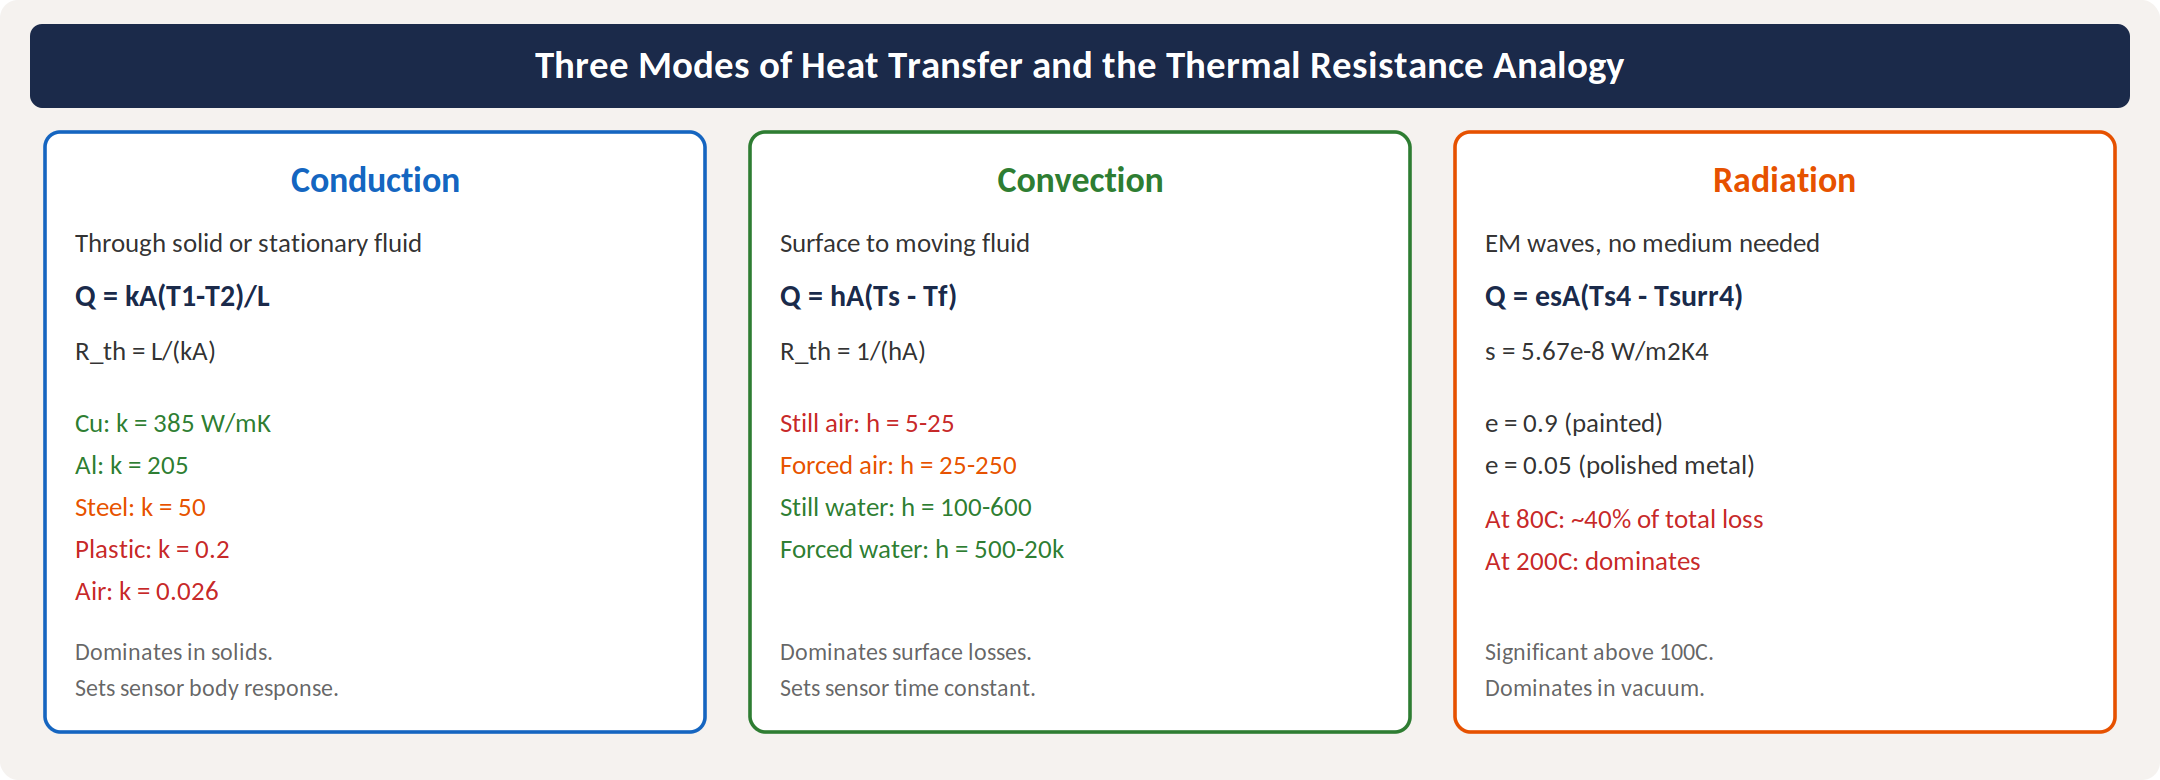
\includegraphics[width=\textwidth]{fig_heat_transfer_modes.png}
\caption{The three modes of heat transfer with typical coefficient values for laboratory conditions. Convection coefficient $h$ varies by three orders of magnitude depending on the fluid and flow conditions, making it the dominant design variable for sensor time constants.}
\label{fig:heat_modes}
\end{figure}


\section{Conduction}
Conduction is heat transfer through a material by molecular vibration and free electron transport, without bulk motion of the material. Fourier's law for one-dimensional steady-state conduction through a flat plate:
\begin{equation}
\dot{Q} = -kA\frac{dT}{dx} = kA\frac{T_1 - T_2}{L}
\end{equation}
where $\dot{Q}$ is the heat transfer rate (W), $k$ is the thermal conductivity (W/m$\cdot$K), $A$ is the cross-sectional area (m$^2$), $L$ is the thickness (m), and $T_1 - T_2$ is the temperature difference across the plate. The heat flux (per unit area) is $q = \dot{Q}/A = k(T_1 - T_2)/L$ (W/m$^2$).

\subsection{Thermal Conductivity}
Thermal conductivity varies enormously across materials: copper $k = 385$\,W/m$\cdot$K, aluminum $k = 205$, steel $k = 50$, glass $k = 1.0$, wood $k = 0.15$, polystyrene foam $k = 0.035$, air $k = 0.026$. Metals conduct well (free electrons); insulators conduct poorly (no free electrons, heat transfers by lattice vibrations only).

\subsection{Thermal Resistance}
By analogy to Ohm's law ($V = IR$), define thermal resistance $R_{\text{th}} = L/(kA)$ (K/W). Then $\dot{Q} = \Delta T / R_{\text{th}}$. For layers in series (a wall with insulation): $R_{\text{total}} = R_1 + R_2 + \cdots$. For layers in parallel (fins): $1/R_{\text{total}} = 1/R_1 + 1/R_2 + \cdots$. The thermal resistance analogy allows you to analyze complex heat transfer paths using circuit analysis techniques.

\subsection{Composite Walls}
For a wall with $n$ layers of different materials:
\begin{equation}
\dot{Q} = \frac{T_{\text{hot}} - T_{\text{cold}}}{\sum_{i=1}^{n} L_i/(k_i A)}
\end{equation}
The layer with the highest $R_{\text{th}}$ (lowest $k$ or greatest thickness) dominates the total resistance and limits the heat flow. This is analogous to the dominant contributor in an error budget.

\begin{examplebox}[ThermoRig: Conduction Through the Test Specimen]
The ThermoRig specimen is a 10\,mm thick aluminum plate ($k = 205$\,W/m$\cdot$K) with area $A = 50 \times 50$\,mm $= 0.0025$\,m$^2$. With $\Delta T = 57$\,\degC{} across the plate: $\dot{Q} = 205 \times 0.0025 \times 57 / 0.010 = 2921$\,W. This is very high because aluminum is an excellent conductor. If the specimen were stainless steel ($k = 15$\,W/m$\cdot$K): $\dot{Q} = 15 \times 0.0025 \times 57 / 0.010 = 214$\,W. If acrylic ($k = 0.2$): $\dot{Q} = 2.85$\,W. The material determines whether the 200\,W heater is adequate.
\end{examplebox}

\section{Convection}
Convection is heat transfer between a surface and a moving fluid (gas or liquid). Newton's law of cooling:
\begin{equation}
\dot{Q} = hA(T_s - T_\infty)
\end{equation}
where $h$ is the convection heat transfer coefficient (W/m$^2\cdot$K), $A$ is the surface area, $T_s$ is the surface temperature, and $T_\infty$ is the bulk fluid temperature far from the surface.

\subsection{Natural (Free) Convection}
Fluid motion driven by buoyancy (density differences caused by temperature gradients). Typical $h$ values: still air: 5--25\,W/m$^2\cdot$K. Still water: 20--100\,W/m$^2\cdot$K. Natural convection is the dominant cooling mechanism for electronics enclosures, laboratory apparatus, and any surface exposed to ambient air without forced airflow.

\subsection{Forced Convection}
Fluid motion driven by an external source (fan, pump, wind). Typical $h$ values: forced air (low speed): 25--250\,W/m$^2\cdot$K. Forced air (high speed): 250--1000. Forced water: 100--20{,}000. The dramatic increase in $h$ with forced flow is why fans are essential for cooling power electronics and why stirring a liquid dramatically accelerates heating or cooling.

\subsection{Convective Thermal Resistance}
$R_{\text{conv}} = 1/(hA)$ (K/W). For the ThermoRig specimen surface ($A = 0.0025$\,m$^2$) in still air ($h = 10$\,W/m$^2\cdot$K): $R_{\text{conv}} = 1/(10 \times 0.0025) = 40$\,K/W. In forced air ($h = 100$): $R_{\text{conv}} = 4$\,K/W. The convective resistance can dominate or be negligible depending on the flow conditions.

\begin{tipbox}[Estimating $h$ for Laboratory Conditions]
For back-of-envelope calculations in MEGN~300: $h \approx 10$\,W/m$^2\cdot$K for still air (natural convection, small temperature difference). $h \approx 50$ for gentle airflow from a nearby fan. $h \approx 200$ for direct airflow from a bench fan at 2\,m/s. $h \approx 500$--1000 for water cooling. These estimates are accurate to $\pm$50\%, which is often sufficient for initial design.
\end{tipbox}

\section{Radiation}
Radiation is heat transfer by electromagnetic waves. It requires no medium and is significant at high temperatures or in vacuum. The Stefan-Boltzmann law for a gray body:
\begin{equation}
\dot{Q}_{\text{rad}} = \epsilon \sigma A (T_s^4 - T_{\text{surr}}^4)
\end{equation}
where $\epsilon$ is the emissivity (0--1; $\epsilon = 1$ for a perfect blackbody, $\epsilon \approx 0.9$ for painted surfaces, $\epsilon \approx 0.05$ for polished metal), $\sigma = 5.67 \times 10^{-8}$\,W/m$^2\cdot$K$^4$ is the Stefan-Boltzmann constant, and temperatures are in Kelvin.

\subsection{When Radiation Matters}
At low temperatures ($<$100\,\degC{}), radiation is typically small compared to convection. At 80\,\degC{} ($= 353$\,K) with surroundings at 20\,\degC{} ($= 293$\,K), $\epsilon = 0.9$, $A = 0.0025$\,m$^2$: $\dot{Q}_{\text{rad}} = 0.9 \times 5.67 \times 10^{-8} \times 0.0025 \times (353^4 - 293^4) = 0.9 \times 5.67 \times 10^{-8} \times 0.0025 \times (1.55 \times 10^{10} - 7.37 \times 10^{9}) = 1.0$\,W. Compared to convective loss of $\dot{Q}_{\text{conv}} = 10 \times 0.0025 \times 60 = 1.5$\,W, radiation contributes about 40\% of the total heat loss. At higher temperatures or in vacuum, radiation dominates.

\section{Energy Balance}
The energy balance is the most powerful tool in heat transfer analysis. For any system:
\begin{equation}
\dot{E}_{\text{in}} - \dot{E}_{\text{out}} + \dot{E}_{\text{gen}} = \dot{E}_{\text{stored}}
\end{equation}
At steady state ($\dot{E}_{\text{stored}} = 0$): heat in $=$ heat out. In transient conditions: the imbalance changes the system's thermal energy, which changes its temperature.

\subsection{Steady-State Energy Balance}
For the ThermoRig at steady state at 80\,\degC{}: the heater power input must exactly balance the heat losses (conduction through insulation + convection from surfaces + radiation from surfaces). If total loss is 50\,W: the heater must supply 50\,W continuously. Changing the ambient temperature changes the losses, requiring the controller to adjust heater power.

\subsection{Transient Energy Balance}
During heating or cooling, the rate of temperature change is:
\begin{equation}
mC_p\frac{dT}{dt} = \dot{Q}_{\text{in}} - \dot{Q}_{\text{out}}
\end{equation}
where $m$ is the mass (kg) and $C_p$ is the specific heat capacity (J/kg$\cdot$K). For the ThermoRig aluminum specimen ($m = 0.034$\,kg, $C_p = 900$\,J/kg$\cdot$K) with 200\,W heater power and 50\,W losses:
\begin{equation}
0.034 \times 900 \times \frac{dT}{dt} = 200 - 50 = 150\,\text{W}
\end{equation}
$dT/dt = 150/30.6 = 4.9$\,\degC{}/s. This is the initial heating rate (when losses are small). As the specimen heats up, losses increase and $dT/dt$ decreases, following an exponential approach to steady state.

\subsection{The Lumped Capacitance Model}
When the thermal resistance within the object (conduction) is much smaller than the thermal resistance at the surface (convection), the object's temperature is approximately uniform. This is the \textbf{lumped capacitance} assumption, valid when the Biot number $\text{Bi} = hL_c/k < 0.1$, where $L_c = V/A_s$ is the characteristic length (volume/surface area).

Under lumped capacitance, the transient temperature response to a step change in environment is:
\begin{equation}
T(t) = T_\infty + (T_i - T_\infty)e^{-t/\tau}, \qquad \tau = \frac{mC_p}{hA_s} = \frac{\rho V C_p}{hA_s}
\end{equation}
This is a first-order response with time constant $\tau$. This equation directly connects heat transfer to the dynamic measurement theory of Chapter~3: the sensor's thermal time constant is $\tau = mC_p/(hA_s)$.

\begin{examplebox}[ThermoRig: Thermocouple Time Constant from Heat Transfer]
A Type~K thermocouple bead (diameter $d = 1$\,mm, $\rho = 8600$\,kg/m$^3$, $C_p = 500$\,J/kg$\cdot$K) in stirred water ($h = 500$\,W/m$^2\cdot$K). Volume $V = \pi d^3/6 = 5.24 \times 10^{-10}$\,m$^3$. Surface area $A_s = \pi d^2 = 3.14 \times 10^{-6}$\,m$^2$. Mass $m = \rho V = 4.5 \times 10^{-6}$\,kg. Time constant: $\tau = 4.5 \times 10^{-6} \times 500 / (500 \times 3.14 \times 10^{-6}) = 1.43$\,s. In still air ($h = 10$): $\tau = 71.7$\,s. This explains why thermocouples respond much faster in liquids than in air: the convective resistance dominates and is 50$\times$ lower in stirred water.
\end{examplebox}

\section{Heat Transfer and Sensor Placement}
Where you place the sensor determines what you measure. Temperature is not uniform in most systems; gradients exist due to conduction, convection, and radiation.

\textbf{Surface temperature}: mount the sensor in intimate thermal contact with the surface (thermal paste or epoxy). The sensor measures the surface temperature, not the fluid temperature. Lead wires conduct heat away from the sensor, creating ``fin effects'' that bias the reading toward ambient. Minimize lead wire thermal conduction by using small-diameter wire and routing leads along isotherms (not across temperature gradients).

\textbf{Fluid temperature}: immerse the sensor in the fluid with sufficient depth (at least 10 sensor diameters) to minimize conduction error along the stem. In high-velocity flow, the sensor may measure the stagnation temperature (slightly above the static temperature due to kinetic energy recovery).

\textbf{Contact resistance}: the interface between a sensor and a surface has thermal resistance from air gaps and surface roughness. Contact resistance can be 10$\times$ larger than the sensor's own thermal resistance, dominating the time constant and introducing a temperature offset. Thermal paste (zinc oxide or silicone-based) reduces contact resistance by 5--10$\times$.

\section{Thermal Design for Control Systems}
When designing the ThermoRig PID control system, heat transfer analysis answers critical design questions:

\textbf{Heater power sizing}: at the maximum setpoint ($T_{\text{max}} = 200$\,\degC{}) with worst-case ambient ($T_{\text{amb}} = 15$\,\degC{}), the total heat loss is $\dot{Q}_{\text{loss}} = (h_{\text{conv}} + h_{\text{rad}}) \times A \times (200 - 15)$. Size the heater for at least $1.5 \times \dot{Q}_{\text{loss, max}}$ to ensure the controller has authority to reach the setpoint with margin.

\textbf{Insulation design}: adding insulation reduces $\dot{Q}_{\text{loss}}$, reducing the required heater power and making control easier (smaller disturbance sensitivity). However, insulation also increases the thermal time constant $\tau = mC_p/(h_{\text{eff}}A)$, making the system slower to respond.

\textbf{Achievable bandwidth}: the thermal time constant sets the fundamental speed limit. No controller can make the temperature change faster than the thermal physics allow. For the ThermoRig with $\tau = 30$\,s: the closed-loop bandwidth is limited to approximately $1/(2\pi\tau) = 0.005$\,Hz with P-only control, increased to $\sim$0.05\,Hz with aggressive PID tuning.

\section{Extended Surfaces: Fins}
When natural convection from a surface is insufficient to dissipate the required heat (common in electronics cooling), \textbf{fins} (extended surfaces) increase the effective surface area. A typical heatsink is an array of aluminum fins attached to the component's case.

The fin effectiveness depends on the fin parameter $m = \sqrt{hP/(kA_c)}$ where $h$ is the convection coefficient, $P$ is the fin perimeter, $k$ is the fin thermal conductivity, and $A_c$ is the fin cross-sectional area. The fin efficiency $\eta_f$ (ratio of actual heat transfer to the heat transfer if the entire fin were at the base temperature):
\begin{equation}
\eta_f = \frac{\tanh(mL)}{mL}
\end{equation}
where $L$ is the fin length. For $mL < 1$: $\eta_f > 0.76$ (efficient). For $mL > 3$: $\eta_f < 0.33$ (the fin tip is near ambient temperature; the outer portion contributes little). Making fins longer beyond $mL \approx 2.5$ has diminishing returns.

Practical rule for MEGN~300: an aluminum heatsink ($k = 205$\,W/m$\cdot$K) with fins 20\,mm long, 1\,mm thick, in still air ($h = 10$\,W/m$^2\cdot$K): $m = \sqrt{10 \times 0.042/(205 \times 0.001 \times 0.020)} = 3.2$\,m$^{-1}$, $mL = 3.2 \times 0.02 = 0.064$. $\eta_f = 0.9987 \approx 1.0$. The aluminum fin is so conductive that it is essentially isothermal. Fin efficiency only becomes a concern for long fins in high-$h$ environments (forced water cooling) or for low-conductivity fin materials (steel, plastic).

\section{Thermal Time Constants and Sensor Response}
The lumped capacitance time constant $\tau = mC_p/(hA_s)$ directly connects heat transfer to sensor dynamics (Chapter~3). Reducing $\tau$ (faster sensor) requires:

\textbf{Reducing mass} $m$: use smaller sensor elements. A 0.25\,mm diameter thermocouple bead has $8\times$ less mass than a 0.5\,mm bead, and $4\times$ less surface area, giving $2\times$ lower $\tau$.

\textbf{Increasing $h$}: immerse in liquid instead of air, or increase flow velocity. Moving from still air ($h = 10$) to stirred water ($h = 500$) reduces $\tau$ by $50\times$.

\textbf{Increasing $A_s/m$ ratio}: use thin, flat sensor elements rather than bulky probe assemblies. An exposed junction thermocouple ($A_s/m$ ratio limited only by the wire diameter) is faster than a grounded junction in a protective sheath (which adds thermal mass without proportional surface area).

\section{Thermal Interface Materials}
The contact between two solid surfaces is never perfect. Microscopic surface roughness creates air gaps that act as thermal insulators. Contact resistance $R_{\text{contact}} = 1/(h_c A)$ where $h_c$ is the contact conductance, ranging from 3{,}000\,W/m$^2\cdot$K (rough, dry metal surfaces) to 20{,}000\,W/m$^2\cdot$K (smooth, greased surfaces).

Thermal interface materials (TIMs) fill the air gaps:

\textbf{Thermal paste} (silicone + ZnO or Al$_2$O$_3$ particles): $k = 1$--$5$\,W/m$\cdot$K. Most common for electronics. Apply a thin, uniform layer (50--100\,$\mu$m). Too thick: paste itself becomes the resistance.

\textbf{Thermal pads} (silicone sheet with filler): $k = 1$--$6$\,W/m$\cdot$K. Easier to apply than paste; maintains consistent thickness. Slightly higher resistance than paste due to greater thickness.

\textbf{Phase-change materials}: solid at room temperature, soften at operating temperature to fill gaps. $k = 3$--$5$\,W/m$\cdot$K. Used in laptop CPU cooling.

For the ThermoRig thermocouple: attaching the bead to the specimen surface with thermal paste reduces the contact resistance from $\sim$100\,K/W (dry contact) to $\sim$10\,K/W, significantly improving the temperature measurement accuracy and reducing the apparent time constant.

\section{Radiation Shields and View Factors}
In high-temperature applications or vacuum environments, radiation becomes the dominant heat transfer mode. \textbf{Radiation shields} (polished metal foils between hot and cold surfaces) reduce radiative heat transfer by introducing additional resistances in the radiation path. Each shield approximately halves the radiation heat transfer. Three shields reduce it by $\sim$$8\times$.

The \textbf{view factor} $F_{12}$ describes the fraction of radiation leaving surface~1 that reaches surface~2. For two parallel plates: $F_{12} \approx 1$. For a small surface facing a large enclosure: $F_{12} = 1$. For a sensor mounted on a surface facing a room: $F_{12}$ depends on the geometry but is typically 0.5--0.8. The radiation exchange between surfaces 1 and 2:
\begin{equation}
\dot{Q}_{12} = \sigma A_1 F_{12} \frac{T_1^4 - T_2^4}{1/\epsilon_1 + A_1/A_2(1/\epsilon_2 - 1)}
\end{equation}

For MEGN~300 applications at moderate temperatures ($< 200$\,\degC{}), the simplified form $\dot{Q}_{\text{rad}} = \epsilon\sigma A(T_s^4 - T_{\text{surr}}^4)$ with $\epsilon$ as the surface emissivity is usually sufficient.

\section{Dimensional Analysis and Nusselt Number}
In advanced heat transfer, the convection coefficient $h$ is predicted using dimensionless correlations. The \textbf{Nusselt number} $\text{Nu} = hL/k_{\text{fluid}}$ is the dimensionless heat transfer coefficient. It depends on the \textbf{Reynolds number} $\text{Re} = \rho v L / \mu$ (forced convection) or the \textbf{Rayleigh number} $\text{Ra} = g\beta\Delta T L^3/(\nu\alpha)$ (natural convection).

For natural convection from a vertical plate: $\text{Nu} = 0.59 \, \text{Ra}^{1/4}$ for $10^4 < \text{Ra} < 10^9$. This allows you to estimate $h$ from the geometry and temperature difference without experimental measurement.

While you will not need to use these correlations for MEGN~300 labs (the empirical $h$ estimates are sufficient), understanding that $h$ can be predicted from fluid mechanics principles connects instrumentation to your heat transfer coursework.
\section{Heat Transfer Coefficient Estimation}
For back-of-envelope calculations without solving the full convection equations, use these empirical correlations:

\textbf{Natural convection from a vertical plate} (laminar, $\text{Ra} < 10^9$):
\begin{equation}
h \approx 1.42 \left(\frac{\Delta T}{L}\right)^{0.25} \text{ W/m}^2\text{K (in air)}
\end{equation}
For a 100\,mm plate at $\Delta T = 50$\,\degC{}: $h \approx 1.42 \times (50/0.1)^{0.25} = 1.42 \times 4.73 = 6.7$\,W/m$^2\cdot$K.

\textbf{Forced convection over a flat plate} (turbulent, $\text{Re} > 5 \times 10^5$):
\begin{equation}
h \approx 0.037 \frac{k_{\text{air}}}{L} \text{Re}^{0.8} \text{Pr}^{0.33}
\end{equation}
For air at 2\,m/s over a 100\,mm plate: $\text{Re} = 1.2 \times 2 \times 0.1 / (1.8 \times 10^{-5}) = 13{,}333$ (laminar). Use the laminar correlation instead: $h \approx 0.664 \times (0.026/0.1) \times 13333^{0.5} \times 0.71^{0.33} = 0.172 \times 115.5 \times 0.89 = 17.7$\,W/m$^2\cdot$K.

\section{Transient Heating and Cooling Curves}
The lumped capacitance model produces exponential heating/cooling curves that directly determine measurement system behavior:

\textbf{Heating}: $T(t) = T_{ss} - (T_{ss} - T_i)e^{-t/\tau}$ where $T_{ss} = T_{\text{amb}} + \dot{Q}_{\text{heater}}/(hA)$ is the steady-state temperature and $\tau = mC_p/(hA)$.

\textbf{Cooling} (heater off): $T(t) = T_{\text{amb}} + (T_i - T_{\text{amb}})e^{-t/\tau}$.

The time to reach a target temperature (within $\delta$ of $T_{ss}$): $t_{\text{settle}} = \tau \ln((T_{ss} - T_i)/\delta)$. For $T_i = 22$\,\degC{}, $T_{ss} = 80$\,\degC{}, $\delta = 0.5$\,\degC{}: $t = \tau \ln(58/0.5) = 4.76\tau$. With $\tau = 30$\,s: $t = 143$\,s $\approx 2.4$\,minutes to settle within 0.5\,\degC{} of setpoint.

\section{Multi-Node Thermal Models}
When the lumped capacitance assumption is not valid ($\text{Bi} > 0.1$), the system must be modeled with multiple thermal nodes, each with its own temperature. The ThermoRig with a thick steel specimen might require three nodes: (1) heater surface, (2) specimen center, (3) specimen surface exposed to air.

Each node has a thermal capacitance $C_i = m_i C_{p,i}$ and is connected to adjacent nodes by thermal resistances $R_{ij}$. The energy balance for each node:
\begin{equation}
C_i \frac{dT_i}{dt} = \sum_j \frac{T_j - T_i}{R_{ij}} + \dot{Q}_{i,\text{ext}}
\end{equation}
This system of ODEs can be solved in LabVIEW using the ``ODE Solver'' VI, MATLAB's \texttt{ode45}, or a simple Euler integration in a While Loop.

The multi-node model reveals internal temperature gradients. The heater surface may be at 120\,\degC{} while the measurement surface is at 80\,\degC{}. If the thermocouple is on the measurement surface, the controller ``sees'' 80\,\degC{}, but the heater is already at its thermal limit. This mismatch between the controlled variable and the constraint variable is a common cause of heater failure in poorly designed thermal systems.
\section{Practice Questions}
\begin{enumerate}[leftmargin=1.5em]
\item A steel plate ($k = 50$\,W/m$\cdot$K) is 5\,mm thick with area 100\,cm$^2$. If one face is at 120\,\degC{} and the other at 80\,\degC{}, what is the heat transfer rate?
\item The ThermoRig specimen (aluminum, $m = 34$\,g, $C_p = 900$\,J/kg$\cdot$K) is heated by a 100\,W heater in still air ($h = 10$\,W/m$^2\cdot$K, $A = 50$\,cm$^2$). Write the energy balance and find the steady-state temperature (ambient: 22\,\degC{}).
\item Calculate the Biot number for the thermocouple bead in the worked example. Is the lumped capacitance assumption valid?
\item A copper block ($k = 385$\,W/m$\cdot$K, $\rho = 8960$\,kg/m$^3$, $C_p = 385$\,J/kg$\cdot$K) is a 20\,mm cube cooled by forced air ($h = 100$\,W/m$^2\cdot$K). Calculate the time constant and the time to cool from 100\,\degC{} to within 1\,\degC{} of ambient (25\,\degC{}).
\item Explain why a thermocouple in still air has a time constant 50$\times$ longer than the same thermocouple in stirred water. Which physical parameter changes, and by how much?
\end{enumerate}

\subsection{Answers}
\begin{enumerate}[leftmargin=1.5em]
\item $\dot{Q} = 50 \times 0.01 \times (120-80)/0.005 = 4000$\,W. The thin steel plate conducts very effectively.
\item Energy balance: $100 = 10 \times 0.005 \times (T_{ss} - 22) + \epsilon\sigma \times 0.005 \times (T_{ss}^4 - 295^4)$. Neglecting radiation as first approximation: $100 = 0.05(T_{ss} - 22)$, $T_{ss} = 2022$\,\degC{}. This is clearly too high, the steady state would be limited by the heater surface area and the onset of higher convection at elevated temperatures. In practice, the specimen reaches the heater's surface temperature limit ($\sim$200\,\degC{} for ceramic heaters) and the energy balance includes radiation and increased natural convection ($h$ increases with $\Delta T$). A more realistic $h = 15$\,W/m$^2\cdot$K with radiation ($h_{\text{rad}} \approx 5$ at moderate temperatures): $100 = (15+5) \times 0.005 \times (T_{ss} - 22)$, $T_{ss} = 1022$\,\degC{}. The problem illustrates that 100\,W is far more power than needed for a small specimen in air.
\item $L_c = V/A_s = (5.24 \times 10^{-10})/(3.14 \times 10^{-6}) = 1.67 \times 10^{-4}$\,m. In water ($h = 500$): $\text{Bi} = 500 \times 1.67 \times 10^{-4}/22 = 0.0038 \ll 0.1$. Lumped capacitance is valid ($k_{\text{chromel}} \approx 22$\,W/m$\cdot$K).
\item $V = (0.02)^3 = 8 \times 10^{-6}$\,m$^3$. $A_s = 6 \times (0.02)^2 = 2.4 \times 10^{-3}$\,m$^2$. $m = 8960 \times 8 \times 10^{-6} = 0.0717$\,kg. $\tau = 0.0717 \times 385/(100 \times 2.4 \times 10^{-3}) = 115$\,s. Time to 1\,\degC{} of ambient: $T(t) = 25 + 75e^{-t/115} = 26$\,\degC{} when $75e^{-t/115} = 1$, $t = 115\ln(75) = 115 \times 4.32 = 497$\,s $\approx 8.3$\,min.
\item The time constant $\tau = mC_p/(hA_s)$ is inversely proportional to $h$. Only $h$ changes: from $\sim$10\,W/m$^2\cdot$K in still air to $\sim$500\,W/m$^2\cdot$K in stirred water (50$\times$ increase). All other parameters ($m$, $C_p$, $A_s$) are properties of the thermocouple and do not change with the medium.
\end{enumerate}
\chapter*{References and Further Resources}
\addcontentsline{toc}{chapter}{References and Further Resources}

\section*{Textbooks and Standards}

\begin{enumerate}[label={[\arabic*]},leftmargin=2em]
\item J.~Fraden, \emph{Handbook of Modern Sensors}, 5th~ed., Springer, 2016.
\item R.~S.~Figliola and D.~E.~Beasley, \emph{Theory and Design for Mechanical Measurements}, 6th~ed., Wiley, 2015.
\item P.~R.~Bevington and D.~K.~Robinson, \emph{Data Reduction and Error Analysis for the Physical Sciences}, 3rd~ed., McGraw-Hill, 2003.
\item A.~V.~Oppenheim and R.~W.~Schafer, \emph{Discrete-Time Signal Processing}, 3rd~ed., Pearson, 2010.
\item S.~W.~Smith, \emph{The Scientist and Engineer's Guide to Digital Signal Processing}, California Technical Publishing, 1997 (free online at dspguide.com).
\item P.~Horowitz and W.~Hill, \emph{The Art of Electronics}, 3rd~ed., Cambridge University Press, 2015.
\item K.~J.~\r{A}str\"{o}m and R.~M.~Murray, \emph{Feedback Systems: An Introduction for Scientists and Engineers}, 2nd~ed., Princeton University Press, 2020 (free online at fbswiki.org).
\item JCGM, ``Evaluation of measurement data: Guide to the expression of uncertainty in measurement (GUM),'' JCGM~100:2008.
\item R.~C.~Dorf and R.~H.~Bishop, \emph{Modern Control Systems}, 13th~ed., Pearson, 2016.
\item National Instruments, ``NI DAQ Hardware Documentation,'' ni.com, accessed 2025.
\item B.~C.~Kuo and F.~Golnaraghi, \emph{Automatic Control Systems}, 10th~ed., McGraw-Hill, 2017.
\item G.~F.~Franklin, J.~D.~Powell, and A.~Emami-Naeini, \emph{Feedback Control of Dynamic Systems}, 8th~ed., Pearson, 2019.
\end{enumerate}

\section*{Free Online Resources}
\begin{itemize}[leftmargin=1.5em]
\item \textbf{DSP}: S.~W.~Smith, \emph{The Scientist and Engineer's Guide to DSP}, free at \url{https://dspguide.com}
\item \textbf{Control}: \r{A}str\"{o}m \& Murray, \emph{Feedback Systems}, free at \url{https://fbswiki.org}
\item \textbf{Fourier intuition}: 3Blue1Brown, ``But what is the Fourier Transform?'' (YouTube)
\item \textbf{PID tuning}: MATLAB Tech Talks, ``Understanding PID Control'' series (YouTube)
\item \textbf{NI DAQ}: NI Developer Zone tutorials at \url{https://ni.com/docs}
\item \textbf{Op-amp design}: Texas Instruments, ``Analog Engineer's Pocket Reference'' (free PDF)
\item \textbf{Filter design}: Analog Devices Filter Wizard at \url{https://tools.analog.com/en/filterwizard/}
\item \textbf{PCB/electronics}: EEVblog YouTube channel (practical electronics tutorials)
\end{itemize}

\end{document}
